\RequirePackage{bookml/bookml-init}
\documentclass[10pt,oneside]{book}

% BookML/LaTeXML reads the same chapter sources as the PDF edition.
\usepackage{bookml/bookml}
\iflatexml\else\usepackage{xeCJK}\fi
\usepackage{listings}
\lstset{upquote=true}
\usepackage{xcolor}
\usepackage{graphicx}
\usepackage{longtable}
\usepackage{makecell}
\usepackage{multirow}
\usepackage{colortbl}
\usepackage{enumitem}
\usepackage{framed}
\usepackage[colorlinks,linktoc=page,allcolors=linkcolor]{hyperref}
\usepackage{bookmark}
\usepackage{pifont}

\definecolor{linkcolor}{RGB}{175, 74, 87}
\definecolor{tablecolor}{RGB}{241, 246, 252}
\setlist{nosep}
\renewcommand{\thetable}{\thechapter{}-\arabic{table}}
\renewcommand{\tablename}{表}
\providecommand{\tableautorefname}{表}
\renewcommand{\tableautorefname}{表}
\renewcommand{\thefigure}{\thechapter{}-\arabic{figure}}
\renewcommand{\figurename}{图}
\providecommand{\figureautorefname}{图}
\renewcommand{\figureautorefname}{图}

\newenvironment{note}{%
  \begin{framed}\begin{center}\textbf{NOTE}\end{center}%
}{\end{framed}}
\newcommand{\codeentry}[1]{\begin{flushleft}\emph{\texttt{#1}}\end{flushleft}}
\newcommand{\hangparagraph}[1]{\noindent #1}

\title{Programming Rust, 2nd Edition}
\author{Jim Blandy, Jason Orendorff, Leonora F. S. Tindall}

\begin{document}
\frontmatter
\begin{titlepage}
  \centering
  {\Huge\bfseries Programming Rust, 2nd Edition\par}
  \vspace{1em}
  {\Large Fast, Safe Systems Development\par}
  \vspace{2em}
  {作者: Jim Blandy, Jason Orendorff, Leonora F. S. Tindall\par}
  \vspace{1em}
  {译者：\href{https://github.com/MeouSker77/ProgrammingRust}{MeouSker77}\par}
  \vspace{1em}
  {版本：\href{https://www.oreilly.com/library/view/programming-rust-2nd/9781492052586/}{2021-06-11}\par}
\end{titlepage}
\setcounter{secnumdepth}{0}
\tableofcontents
\chapter{前言}
Rust是一门为系统级编程设计的语言。

因为很多业务程序员对系统级编程并不是很熟悉,所以这里解释一下,它是我们所做的一切的基础。

当你合上笔记本电脑时,操作系统检测到了这一行为,然后把所有正在运行的程序挂起、关掉屏幕、并把电脑设置为睡眠。之后,当你打开笔记本电脑时:屏幕和其他组件被再次唤醒,并且每个程序可以在它中断的地方继续运行。我们对此习以为常。但系统程序员为此编写了很多代码。

系统级编程被用于以下领域:
\begin{itemize}
    \item 操作系统
    \item 各种设备的驱动
    \item 文件系统
    \item 数据库
    \item 在非常廉价或需要极高的可靠性的设备上运行的代码
    \item 密码学
    \item 多媒体编解码器(用于读写音频、视频、图片文件的软件)
    \item 多媒体处理(例如,语音识别或图像处理软件)
    \item 内存管理(例如,实现一个垃圾回收器)
    \item 文本渲染(把文本和字体转换为像素点的过程)
    \item 实现更高级的编程语言(例如JavaScript和Python)
    \item 网络
    \item 虚拟化和容器
    \item 科学仿真
    \item 游戏
\end{itemize}

简而言之,系统级编程是一种\emph{资源受限}的编程方式,它是一种每一个字节和每一个CPU时钟都需要考虑的编程方式。为了支持一个基本的应用所需要的系统级代码的数量是非常惊人的。

本书并不会教你系统级编程。事实上,这本书包含了很多有关内存管理的细节,如果你没有自己进行过系统级编程,你会感觉这些内容乍一看似乎没有必要。但如果你是一个熟练的系统级程序员,你将会发现Rust是一门非常优秀的语言:它是一件可以解决困扰了整个工业界几十年的主要问题的工具。

\section*{谁应该阅读这本书}
如果你已经是一名系统级程序员并且已经准备好替换C++,那么这本书就是为你而生。如果你是一名有其他任何语言的经验的开发者,不管是C\#、Java、Python、JavaScript还是其他语言,这本书同样适用于你。

然而,你不仅需要学习Rust。为了充分利用这门语言,你还需要获取一些系统级编程的经验。我们推荐在阅读这本书的同时用Rust实现一些系统编程的项目,构建一些你以前从来没有构建过的东西、一些充分利用Rust的速度、并发和安全性的东西。本前言开头的列表也许能给你一些启发。

\section*{我们为什么要撰写这本书}
早在我们开始学习Rust时我们就开始着手编写这本书。我们的目标是首先正面处理Rust中主要的、新的概念,清晰而深入地呈现它们,以最大限度地避免通过试错来学习。

\section*{本书概览}
本书的前两章介绍了Rust,并提供了一个简单的示例。之后我们转到\hyperref[ch03]{第3章}的基本数据类型。\hyperref[ch04]{第4章}、\hyperref[ch05]{第5章}专注于介绍所有权和引用的核心概念。我们推荐按照顺序阅读前5章。

第\hyperref[ch06]{6}到第\hyperref[ch10]{10}章覆盖了语言的基础部分:表达式(\hyperref[ch06]{第6章}),错误处理(\hyperref[ch07]{第7章}),crate和模块(\hyperref[ch08]{第8章}),结构体(\hyperref[ch9]{第09章}),枚举和模式(\hyperref[ch10]{第10章})。在这一部分可以跳过一些内容,但请相信我们,不要跳过错误处理的章节。\hyperref[ch11]{第11章}包括trait和泛型,这是最后两个你需要知道的重要概念。trait类似于Java或C\#中的接口。它们也是Rust支持把你自己的类型集成到语言中的主要手段。\hyperref[ch12]{第12章}展示了trait怎么支持运算符重载,\hyperref[ch13]{第13章}包括了很多有用的工具trait。

理解了trait和泛型就可以解锁本书的剩余部分了。闭包和迭代器,这两个你绝对不想错过的强大工具,分别在\hyperref[ch14]{第14章}和\hyperref[ch15]{第15章}中介绍。你可以以任意顺序阅读剩下的章节,或者按需阅读。它们包括了剩余的语言部分:集合(\hyperref[ch16]{第16章}),字符串和文本(\hyperref[ch17]{第17章}),输入和输出(\hyperref[ch18]{第18章}),并发(\hyperref[ch19]{第19章}),异步代码(\hyperref[ch20]{第20章}),宏(\hyperref[ch21]{第21章}),unsafe代码(\hyperref[ch22]{第22章})和调用其它语言中的函数(\hyperref[ch23]{第23章})。

\section*{本书中的约定}
本书中用到了以下约定:

\hangafter 1
\hangindent 2em
\noindent
\emph{斜体}\\
表示新术语、URL、电子邮件地址、文件名和文件拓展名。

\hangafter 1
\hangindent 2em
\noindent
\texttt{等宽}\\
用于代码环境和在段落中引用代码中的元素例如变量或函数名、数据库、数据类型、环境变量、语句和关键字等。

\hangafter 1
\hangindent 2em
\noindent
\textbf{\texttt{等宽加粗}}\\
表示需要用户逐字输入的命令或其他文本。

\hangafter 1
\hangindent 2em
\noindent
\emph{\texttt{等宽斜体}}\\
表示需要用户用自己的值或者上下文推断出的值进行替换的文本。

\begin{note}
    这个标志表示一个注意事项。
\end{note}

\section*{使用示例代码}
补充材料(示例代码,练习等)可以在\url{https://github.com/ProgrammingRust}下载。

本书旨在帮助你完成工作。一般来说,本书中提供的示例代码,你可以在自己的编程和文章中使用。除非你需要再次分发大量本书中的代码,否则你不需要联系我们获取授权。例如,编写一个使用了书中部分代码的程序并不需要授权。售卖或者分发O'Reilly书籍中的示例代码则需要授权。通过引用本书或书中的示例代码回答问题并不需要授权。将本书中的大量代码纳入你自己的产品文档则需要授权。

我们感激,但并不要求署名。如果要署名的话,应该包含标题、作者、出版社和ISBN。例如:“Programming Rust, Second Edition by Jim Blandy, Jason Orendorff, and Leonora F.S. Tindall(O’Reilly). Copyright 2021 Jim Blandy, Leonora F.S. Tindall, and Jason Orendorff, 978-1-492-05259-3.”

如果你感觉你对示例代码的使用方式不在上述范围内,请放心联系我们\url{permissions@oreilly.com}。

\section*{O'Reilly在线学习}
\begin{note}
    40多年以来,O'Reilly Media提供技术和业务培训、知识和洞察力,以帮助公司取得成功。
\end{note}

我们独特的专家和创意网络会通过书籍、文章、会议和在线学习平台分享他们的知识。O'Reilly的在线学习平台可以让你按需访问O'Reilly及其他200多家出版社的实时培训课程、深入学习路线、交互式代码环境。更多信息请访问\url{http://oreilly.com}。

\section*{如何联系我们}
请将和本书有关的评论和问题发送给出版社:

\hangafter 0
\hangindent 3em
\noindent
\large{O'Reilly Media, Inc.}\\
\large{1005 Gravenstein Highway North}\\
\large{Sebastopol, CA 95472}\\
\large{800-998-9938 (in the United States or Canada)}\\
\large{707-829-0515 (international or local)}\\
\large{707-829-0104 (fax)}

我们有一个本书的web页面,我们在那里列出了勘误表、示例和其他附加信息。你可以通过\url{https://oreil.ly/programming-rust-2e}访问该页面。

评论或有关本书的技术问题可以发送到邮箱\url{bookquestions@oreilly.com}。

访问\url{http://www.oreilly.com}获取更多有关我们的书籍和课程的信息。

我们的Facebook:\url{http://facebook.com/oreilly}

我们的Twitter:\url{http://twitter.com/oreillymedia}

我们的YouTube:\url{http://youtube.com/oreillymedia}

\section*{致谢}
你手中的这本书从我们的官方技术评审:Brian Anderson、Matt Brubeck、J. David Eisenberg、Ryan Levick、Jack Moffitt、Carol Nichols、Erik Nordin和翻译:Hidemoto Nakada (中田 秀基) (Japanese)、Mr. Songfeng Li (Simplified Chinese)、Adam Bochenek和Krzysztof Sawka (Polish)处受益匪浅。

还有很多非官方的评审阅读了早期的草案并提供了很有价值的反馈。我们想要感谢Eddy Bruel、Nick Fitzgerald、Graydon Hoare、Michael Kelly、Jeffrey Lim、Jakob Olesen、Gian-Carlo Pascutto、Larry Rabinowitz、Jaroslav Šnajdr、Joe Walker、Yoshua Wuyts的认真评论。
Jeff Walden和NicolasPierron花费了宝贵的时间来审阅几乎整本书。就像编程一样,一本编程书籍需要高质量的bug报告才能不断成长。感谢你们。

Mozilla对Jim和Jason在此项目中的工作非常宽容,尽管这超出了我们的官方职责范围,并会和他们产生竞争。我们非常感谢Jim和Jason的领导:Dave Camp、Naveed Ihsanullah、Tom Tromey、Joe Walker的支持。他们从长远的角度看待Mozilla,我们希望这些结果证明了他们对我们的信任。

我们还想对O'Reilly里每个帮助过我们的人表达感谢,尤其是非常有耐心的编辑Jeff Bleiel和Brian MacDonald,以及我们的策划编辑Zan McQuade。

最重要的是,我们衷心感谢家人们坚定不移的爱、热情和耐心。
\chapter{译者序}
这是我翻译的第二本英文资料。

\section*{相识}
初次听说Rust的传闻还是大二时候听说有位清华的大佬用Rust实现了自己的编译器和操作系统作为毕设，当时虽然不懂但大为震撼（笑）。
初次接触Rust应该还是大三，当时是看官方的书入门的。
但我相信一定有很多人和我一样，看完官方的书之后合上书发现自己其实还是什么也写不出来（笑）。

初次接触本书是在21年7月初从Rust中文社区的推送消息中得知，当发现本书有一千多页时推测本书应该是类似C/C++ Primer [Plus]那样的比较全面的书籍，事实果然如此。
不过因为当时忙于科研，没有空余时间阅读本书，就一直搁置了下去（实名吐槽某实验室让大四刚毕业的学生搞科研搞到8月份才能放暑假回家）。

初次开始阅读和翻译本书是在2021.9.19日，撰写本序是在2022.9.18日晚，历时恰好一年完成了本书的翻译，不得不感叹命运总是如此巧妙。（整整一年，鬼知道我这一年都经历了什么。）

\section*{相知}
研一刚开学之后忙于科研，到9月下旬才有时间开始翻译，之后连续翻译了几个月，直到快到21年底的时候科研任务又紧张起来才中断了翻译。
再之后就是寒假前后才又有时间继续翻译，在寒假结束之后开学不久我就做出了人生中也许是第二大也是第二正确的选择，随之而来的又是很长一段时间的翻译中断。
终于在22年9月重新拾起了翻译，坚持到了最后。

在翻译本书的前期，我最大的感受只有两个字——绝望。
一千多页的压力让我几乎窒息，即使我每天把所有的时间用来翻译，也只能翻译20-30页，而当时研一的我科研任务繁重，经常每天只能抽出一两个小时来进行翻译，结果就是每天只能翻译几页。
也只有在周末，才能拿出全天时间来翻译，但也只能翻译20-30页。
就这样持续了两周之后，突然发现自己坚持了两周把每天所有空闲时间都拿来翻译，竟然只翻译了$\frac{1}{5}$还不到？
再加上科研压力越来越大，翻译的时间越来越短，绝望之感尤甚。

还记得心态的转变是在翻译到了$\frac{1}{3}$左右的时候，就像是看到了曙光一样，第一次有了自己可以翻译完这本书的信心。
也是从那时起我不再经常犹豫是否还要继续翻译下去。
在那之前我也深刻地感受到了坚持做一件看不到希望的事情是多么痛苦。

22年5月于Rust中文社区推送的消息中得知已有人完成了本书的翻译，当时我离弃坑就差那么亿点点的距离：
直到那时本译文仍然几乎无人问津，且我已经明白了我以后的工作是不可能用到Rust的，既然我已用不到Rust而且本书也有人翻译过了，那我为什么还要继续下去？继续学习Rust和翻译本书对我而言又有什么意义？
幸运的是我很快就得到了这个问题的答案，再加上强迫症的影响，我还是决定继续下去。

\section*{尾声}
本书于2022.9.18日完成翻译（除了第17章不打算进行翻译），在完成时我感受到的并非是完成了一项艰难的任务之后的成就感和幸福感，而是一种平静和释然的感觉。成就感和幸福感不能说没有，只能说是被一年的时长稀释了，留下的只有平淡如水的心境，似乎翻译逐渐成为了习惯、成为了一有空闲时间就会选择的消磨时间的方式。

我在翻译的过程中可以说是收获满满，（虽然长达一年的时长让我已经几乎完全忘记了自己的收获，笑），希望阅读本书的你也能有所收获。

\begin{flushright}
    ——汪屹硕（MeouSker77）

    （真正的实名，笑）

    2022.9.18
\end{flushright}

\section*{致谢}
感谢所有在github上star、fork、issue、pr的读者，你们对本译文的关注和支持也是我坚持下去的主要动力之一。

\mainmatter
\setcounter{secnumdepth}{2}
\chapter{系统级程序员的福音}\label{ch01}
\emph{在某些场景下——例如Rust的目标场景——比竞争对手快10x或者仅仅2x是足以决定成败的事情。它决定了一个系统在市场中的命运，就像在硬件市场中一样。}
\begin{flushright}
    ——Graydon Hoare
\end{flushright}

\emph{现在所有的计算机都是并行的……并行编程才是编程。}
\begin{flushright}
    ——Michael McCool et al., Structured Parallel Programming    
\end{flushright}

\emph{民族国家的攻击者们利用TrueType解析器的漏洞来进行监视；所有的软件都对安全很敏感。}
\begin{flushright}
    ——Andy Wingo
\end{flushright}

我们选择用以上三个引言来开始本书是有原因的。但首先让我们以一个谜题开始。下面的C程序做了什么？
\begin{minted}{C}
    int main(int argc, char **argv) {
        unsigned long a[1];
        a[3] = 0x7ffff7b36cebUL;
        return 0;
    }
\end{minted}

今天早上在Jim的笔记本电脑上，上面的程序输出了：
\begin{minted}{text}
    undef: Error: .netrc file is readable by others.
    undef: Remove password or make file unreadable by others.
\end{minted}
然后它就崩溃了。如果你在自己的机器上尝试，它的行为可能会不同。这个过程中到底发生了什么呢？

这段代码是有漏洞的。数组\texttt{a}的长度为1，对\texttt{a[3]}的访问，根据C语言标准，是\emph{未定义行为}：

\emph{对于使用不可移植或错误的程序结构或错误的数据的行为，国际标准不做任何要求}

未定义行为不仅仅会导致非预期的结果，语言标准甚至允许程序在这种情况下做\emph{任何事情}。在我们的例子中，把一个特定的值存在特定数组的第4个元素处恰巧破坏了函数的调用栈，因此导致\texttt{main}函数返回时，并没有正常的退出程序，而是跳转到了C标准库里从用户的家目录中的一个文件中读取密码的代码中。这显然是有问题的。

C和C++有几百条避免未定义行为的规则。它们大多都是一些常识：不要访问不应该访问的内存，不要让算术运算溢出，不要除以零等等。然而编译器并不强制这些规则，它没有义务去检测哪怕明目张胆的违反规则的行为。事实上，上述程序编译时不会有错误和警告。避免未定义行为的责任全部落到你，程序员身上。

从经验上讲，我们程序员并不能很好的识别出未定义行为。然而，一个Utah大学的学生，研究员Peng Li修改了C和C++的编译器来让它们在编译时报告它们正在编译的程序中是否含有会导致未定义行为的模式。他发现，几乎所有的程序都有，包括那些公认的优秀项目。想要在C和C++中避免未定义行为就和仅仅知道规则就想赢得国际象棋比赛一样不切实际。

各种偶然的奇怪信息或崩溃可能是质量问题，但自从1988年Morris Worm使用了以下技术把代码从一台机器迁移到另一台机器后，不经意间的未定义行为就是导致安全漏洞的一大原因。

因此C和C++把程序员推到了一个很尴尬的地位：这些语言是系统级编程的工业标准，但它们对程序员的要求却几乎保证崩溃和安全问题源源不断。回答我们的谜题只是抛出了一个更大的问题：我们不能做的更好吗？

\section{Rust帮你扛起责任}
我们的答案对应着我们开头的三个引言。第三个引言引用自一篇报告，这篇报告中，一个叫做Stuxnet的计算机蠕虫在2010年被发现侵入了工业界的设备，并获取了受害计算机的控制权。它只是利用了解析word文档中嵌入的TrueType字体的代码中的未定义行为，没有使用任何其他技术。这段代码的作者显然没有预料到这段代码会被以这种形式利用，这说明不仅仅只有操作系统和服务器需要担心安全问题：任何需要处理来自不受信任来源的数据的软件都可能成为受害者。

Rust语言做了一个简单的保证：如果你的代码通过了编译器的检查，那么它将不会遇到未定义行为。悬垂指针，两次释放，空指针解引用都会在编译期被捕捉到。对数组的引用通过编译期和运行期的双重检查保证安全，当索引越界时，Rust不会像不幸的C语言一样出现缓冲区溢出，而是会安全的退出程序并打印出错误消息。

Rust旨在同时实现\emph{安全}和\emph{易于使用}。为了对你的程序行为做出更强的保证，Rust对你的代码施加了比C和C++更多的限制，这些限制需要通过一些实践和经验才能习惯。但总体来看这门语言的灵活性和表达力都是很强的。Rust的应用范围之广已经证明了这一点。

根据我们的经验，在相信语言可以帮助我们捕获错误的情况下，我们将有勇气尝试更有挑战性的项目。修改庞大的、复杂的程序将不会有很大风险，因为不需要关注内存管理和指针有效性的问题。调试起来也会简单得多，因为潜在的bug不会出现在不相关的部分。

当然，还有很多Rust也不能检测出的bug。但在实践中，没有未定义行为可以显著改善开发的现状。

\section{安全的并发编程}
在C和C++中并发是众所周知的难，开发者通常只有在已经证明了单线程代码无法达到所需性能的情况下才会考虑并发。但第二个引言则认为并行非常重要以至于现代计算机将它视为基本的操作。

事实证明，Rust中保证内存安全的限制也可以保证Rust程序中不会出现数据竞争。你可以在线程间安全的共享数据，只要它不是正在被修改。被修改的数据只能通过同步原语来访问。所有传统的工具都可以使用：自旋锁、条件变量、通道、原子量等等。Rust会通过检查确保你正确地使用它们。

这些使Rust能够充分利用现代多核机器的性能。Rust的生态还提供了普通并发原语之外的库来帮助你完成复杂的负载，包括处理器池、无锁同步机制例如Read-Copy-Update等。

\section{Rust的速度很快}
最后，对应我们的第一条引言。Rust遵循了Bjarne Stroustrup在他的文章“Abstraction and the C++ Machine Model”中提到的为C++设计的原则：

\emph{一般情况下，C++的实现遵循0开销原则：你没有用到的部分，将不会有开销。你用到的部分，你将不能找到更好的代码。}

系统级编程经常需要关注将机器性能发挥到极限。对于视频游戏，整个机器都需要投入工作来为玩家创造出最好的体验。对于网页浏览，浏览器的性能制约了内容发布者可以做的上限，在机器本身的限制范围内，需要将尽可能多的内存和处理器资源留给内容本身。同样的原则页也适用于操作系统：内核需要把机器的资源尽可能多的留给用户程序，而不是被它们自身消耗。

但当我们说Rust很“快”的时候，到底是什么意思？一个人可以用任何通用语言写出非常慢的代码。更准确地说，如果你已经准备好认真设计你的程序来最大限度的利用底层机器的性能，那么Rust可以支撑你实现目标。这门语言的效率很高，并且能给予你控制使用多少内存和CPU资源的能力。

\section{Rust使协作变得更简单}
我们在标题中隐藏了第4条引言：“系统级程序员的福音”。这是在暗示Rust对代码共享和重用的支持。

Rust的包管理器和构建工具Cargo，使用户可能很容易的使用其他用户发布在Rust的公开仓库cartes.io上的库。你只需要简单的在一个文件中加上库的名字和版本号，cargo将会自动下载库，和这个库的依赖，并把它们连接在一起。你可以将Rust的Cargo视为NPM或者RubyGems一类的东西，并强调完善的版本控制和可复制的构建。有很多流行的Rust库可以提供从序列化到HTTP客户端和服务器再到现代图形API等几乎任何功能。

进一步讲，这门语言本身就被设计为支持协作：Rust的trait和泛型让你能创建出拥有灵活接口的库，它们可以在很多不同的上下文中工作。Rust的标准库也提供了一组核心的基础类型，为常见的情况建立了共享的约定，使不同的库可以更容易的协同使用。

下一章旨在更具体的说明我们在这一章中提出的观点，我们通过几个小的Rust程序作为示例来展示这门语言的强大之处。
\chapter{Rust概览}\label{ch02}
Rust给像本书一样的书籍的作者提出了一个挑战：赋予这门语言特色的并不是可以在第一页就展示出来的某些惊人的特性，而是如何设计这门语言来让它的各个部分可以无缝的协同工作，最终达到我们在上一章提到的目标：安全、高性能的系统级编程。这门语言的每一部分都在其他所有部分中得到了最好的证明。

因此，相比于一次着眼于一种语言特性，我们选择了几个简单但却完整的程序作为概览，每一个程序都会涉及到一些语言特性：

\begin{itemize}
    \item 作为热身，我们准备了一个简单的计算命令行参数的程序，以及相应的单元测试。这个程序展示了Rust的核心类型，并引入了\emph{trait}。
    \item 接下来，我们构建了一个web服务器。我们将会使用一个第三方库来处理HTTP的细节，并引入字符串处理、闭包、错误处理。
    \item 我们的第三个程序绘制了一个漂亮的图形，讲计算分布到多个线程来提高速度。这一部分包括一个泛型函数的示例，阐明了怎么处理类似于一个像素的概念，并展示了Rust对并发的支持。
    \item 最后，我们展示了一个使用正则表达式处理文件的健壮的命令行程序。这个程序展示了Rust标准库中处理文件的设施，和最常用的第三方正则表达式库。
\end{itemize}

Rust保证在对代码的性能影响最小的情况下防止未定义行为，这一保证影响了整个Rust中每个部分的设计，从标准的数据结构例如vector和string到Rust程序员使用第三方库的方式都受此影响。这些具体的细节书中都会提到，但是现在，我们想向你展示Rust是一门强大且有趣的语言。

当然，首先你要在你的计算机上安装Rust。

\section{rustup和Cargo}
安装Rust的最佳方式是使用\texttt{rustup}。访问\url{https://rustup.rs}并按照说明进行操作。

或者，你可以访问\href{https://www.rust-lang.org/}{Rust网站}来获取预构建好的Linux、macOS、Windows上的包。一些操作系统发行版里也包含Rust。我们推荐\texttt{rustup}，因为它是专用于管理Rust安装的工具，就像Ruby的RVM和Node的NVM一样。例如，当一个新版本的Rust发布时，你只需要输入\texttt{rustup update}就可以完成更新。

在任何情况下，完成了安装之后，你应该可以通过命令行访问以下三条新命令：
\begin{minted}{text}
    $ cargo --version
    cargo 1.49.0 (d00d64df9 2020-12-05)
    $ rustc --version
    rustc 1.49.0 (e1884a8e3 2020-12-29)
    $ rustdoc --version
    rustdoc 1.49.0 (e1884a8e3 2020-12-29)
\end{minted}

这里，\texttt{\$}是命令提示符。在Windows上，可能是\texttt{C:\textbackslash>}或者别的类似的。这里我们运行了安装的三条命令，查询它们的版本。接下来让我们依次讲解每一个命令：
\begin{itemize}
    \item \texttt{cargo}是rust的编译管理器、包管理器和通用的工具。你可以使用Cargo来新建项目、构建并运行程序、管理所有代码中依赖的外部库。
    \item \texttt{rustc}是Rust的编译器。通常我们使用Cargo来调用编译器，但有时也需要直接运行它。
    \item \texttt{rustdoc}是Rust的文档工具。如果你在源代码中按照文档注释的格式写了文档，那么\texttt{rustdoc}可以通过它们构建出漂亮的HTML文档。和\texttt{rustc}一样，我们通常用Cargo来调用\texttt{rustdoc}。
\end{itemize}

方便起见，Cargo可以为我们创建新的Rust包，并设置好一些标准元数据：
\begin{minted}{text}
    $ cargo new hello
        Created binary (application) `hello` package
\end{minted}

这个命令创建了一个叫做\texttt{hello}的新的包目录，并准备好构建一个可执行程序。

进入包的顶级目录并查看：
\begin{minted}{text}
    $ cd hello
    $ ls -la
    total 24
    drwxrwxr-x.  4 jimb jimb 4096 Sep 22 21:09 .
    drwx------. 62 jimb jimb 4096 Sep 22 21:09 ..
    drwxrwxr-x.  6 jimb jimb 4096 Sep 22 21:09 .git
    -rw-rw-r--.  1 jimb jimb    7 Sep 22 21:09 .gitignore
    -rw-rw-r--.  1 jimb jimb   88 Sep 22 21:09 Cargo.toml
    drwxrwxr-x.  2 jimb jimb 4096 Sep 22 21:09 src
\end{minted}

我们可以看到Cargo创建了一个文件\texttt{Cargo.toml}来保存包的元数据。此时这个文件里还没有太多内容：
\begin{minted}{toml}
    [package]
    name = "hello"
    version = "0.1.0"
    authors = ["You <you@example.com>"]
    edition = "2018"

    # See more keys and their definitions at
    # https://doc.rust-lang.org/cargo/reference/manifest.html

    [dependencies]
\end{minted}

如果我们的程序中需要依赖的库，我们可以在这个文件中添加它们，Cargo将会负责下载、构建和更新这些库。我们将在\hyperref[ch08]{第8章}中详细讲述\texttt{Cargo.toml}文件。

Cargo已经为我们的包初始化好了\texttt{git}版本控制系统，创建了一个\texttt{.git}元数据目录和一个\texttt{.gitignore}文件。你可以通过向\texttt{cargo new}命令传递\texttt{--vcs none}参数来跳过这一步。

\texttt{src}子目录包含了实际的Rust代码：
\begin{minted}{text}
    $ cd src
    $ ls -l
    total 4
    -rw-rw-r--.  1 jimb jimb 45 Sep 22 21:09 main.rs
\end{minted}

看起来Cargo好像已经替我们写好了程序。\texttt{main.rs}中包含以下文本：
\begin{minted}{Rust}
    fn main() {
        println!("Hello, world!");
    }
\end{minted}

在Rust中，你甚至不需要编写自己的“Hello, World!”程序，这是新的Rust程序的模板：两个文件，总共13行。

我们可以从包中的任何目录调用\texttt{cargo run}命令来构建并运行我们的程序：
\begin{minted}{text}
    $ cargo run
        Compiling hello v0.1.0 (/home/jimb/rust/hello)
        Finished dev [unoptimized + debuginfo] target(s) in 0.28s
        Running `/home/jimb/rust/hello/target/debug/hello`
    Hello, world!
\end{minted}

这里，Cargo调用了Rust的编译器\texttt{rustc}，然后运行了它生成的可执行文件。Cargo把可执行文件放在了顶层目录的\texttt{target}子目录下：
\begin{minted}{text}
    $ ls -l ../target/debug
    total 580
    drwxrwxr-x. 2 jimb jimb   4096 Sep 22 21:37 build
    drwxrwxr-x. 2 jimb jimb   4096 Sep 22 21:37 deps
    drwxrwxr-x. 2 jimb jimb   4096 Sep 22 21:37 examples
    -rwxrwxr-x. 1 jimb jimb 576632 Sep 22 21:37 hello
    -rw-rw-r--. 1 jimb jimb    198 Sep 22 21:37 hello.d
    drwxrwxr-x. 2 jimb jimb     68 Sep 22 21:37 incremental
    $ ../target/debug/hello
    Hello, world!
\end{minted}

如果需要的话，Cargo可以为我们清理生成的文件：
\begin{minted}{text}
    $ cargo clean
    $ ../target/debug/hello
    bash: ../target/debug/hello: No such file or directory
\end{minted}

\section{Rust函数}
Rust的语法借鉴自其他语言。如果你熟悉C、C++、Java或者JavaScript，你可以很快找到自己的方式来理解Rust的程序结构。这里有一个使用\href{https://en.wikipedia.org/wiki/Euclidean_algorithm}{欧几里得算法}计算两个整数的最大公约数的函数。你可以把它添加到\texttt{src/main.rs}的最后：
\begin{minted}{Rust}
    fn gcd(mut n: u64, mut m: u64) -> u64 {
        assert!(n != 0 && m != 0);
        while m != 0 {
            if m < n {
                let t = m;
                m = n;
                n = t;
            }
            m = m % n;
        }
        n
    }
\end{minted}

\texttt{fn}关键字（读作“fun”）创建了一个函数。这里，我们定义了一个叫\texttt{gcd}的函数，它有两个参数\texttt{m}和\texttt{n}，类型都是\texttt{u64}，也就是64位无符号整数。\texttt{->}词元指明了返回值类型：我们的函数返回一个\texttt{u64}类型的值。四个空格缩进是Rust的标准风格。

Rust的整数类型的名字代表了它们的大小和符号性：\texttt{i32}是有符号32位整数；\texttt{u8}是无符号8位整数（用于“字节”值）等等。\texttt{isize}和\texttt{usize}类型分别代表可以存下一个指针的有符号和无符号整数，在32位平台上它们就是32位，在64位平台上就是64位。Rust还有两种浮点数类型：\texttt{f32}和\texttt{f64}，分别是IEEE标准的单精度和双精度浮点数类型，类似于C和C++中的\texttt{float}和\texttt{double}。

默认情况下，当变量初始化后，它的值就不能再被改变，但通过在参数\texttt{m}和\texttt{n}前加上\texttt{mut}关键字（读作“mute”，\emph{mutable}的缩写）就可以在函数体中对它们进行赋值。在实践中，大多数变量都不会被重新赋值，在阅读代码时\texttt{mut}关键字将是一个有用的提示。

函数体中首先调用了\texttt{assert!}宏，确保两个参数都不是0。\texttt{!}字符标志着这是宏调用，而不是函数调用。类似于C和C++中的\texttt{assert}宏，Rust中的\texttt{assert!}宏也会检查参数是否为真，如果不为真则中断程序，并输出一条有用的信息，其中包括断言失败的源码位置。这种终止的方式被称为\emph{panic}。和C和C++中断言可以被跳过不同，Rust总是检查断言，不管程序怎么编译。还有一个\texttt{debug\_assert!}宏，当程序被编译为release模式时会被跳过。

我们函数的主体是一个包含一条\texttt{if}语句和一条赋值语句的\texttt{while}循环。和C和C++不同，Rust的条件表达式不需要括号，但紧随其后的控制流语句需要花括号。

\texttt{let}语句声明了一个局部变量，比如函数中的\texttt{t}。我们不需要写出\texttt{t}的类型，因为Rust可以通过使用这个值的方式来推断它的类型。在我们的函数中，\texttt{t}只有和\texttt{m}、\texttt{n}相匹配，是\texttt{u64}类型时才可以正常运行。Rust只在函数体内推断类型：你必须写出函数参数和返回值的类型，就像我们所做的那样。如果你想指明\texttt{t}的类型，你可以写：
\begin{minted}{Rust}
    let t: u64 = m;
\end{minted}

Rsut有\texttt{return}语句，但是\texttt{gcd}函数并不需要。如果一个函数体以一个\emph{没有}分号结尾的表达式结尾，那么这个表达式的值就是函数的返回值。事实上，任何一个花括号包围的语法块都可以作为一个表达式。例如，这里有一个表达式打印出一条消息，然后返回\texttt{x.cos()}作为它的值：
\begin{minted}{Rust}
    {
        println!("evaluating cos x");
        x.cos()
    }
\end{minted}

在Rust中当控制流到达函数底部时利用这种形式返回值是一种很典型的做法，只有当在函数的中途显式地返回时才会使用\texttt{return}语句。

\section{编写并运行单元测试}
Rust语言内建有对测试的支持。为了测试我们的\texttt{gcd}函数，我们可以在\texttt{src/main.rs}的最后添加下列代码：
\begin{minted}{Rust}
    #[test]
    fn test_gcd() {
        assert_eq!(gcd(14, 15), 1);

        assert_eq!(gcd(2 * 3 * 5 * 11 * 17,
                       3 * 7 * 11 * 13 * 19),
                   3 * 11);
    }
\end{minted}

这里我们定义了一个叫\texttt{test\_gcd}的函数，它调用了\texttt{gcd}函数并检查返回值是否正确。喊函数上方的\texttt{\#[test]}标记\texttt{test\_gcd}是一个测试函数，这种函数在正常编译时会被跳过，但在使用\texttt{cargo test}命令时会被编译并自动调用。我们可以在整个源码树的任何位置定义测试函数，\texttt{cargo test}会自动收集它们并运行。

\texttt{\#[test]}标记是\emph{属性}的是一个示例。属性是一种为函数和其他声明标记额外信息的开放式系统，类似于C++和C\#中的属性，或者Java中的注解。它们被用来控制编译器警告和代码风格检查、条件编译（类似于C和C++中的\texttt{\#ifdef}）、告诉Rust怎么和其它语言编写的代码交互等。随着继续深入我们将会看到更多使用属性的例子。

把\texttt{gcd}和\texttt{test\_gcd}函数的定义添加到\texttt{hello}包里之后，我们可以在包内的某个目录下按照如下方式运行测试：
\begin{minted}{text}
    $ cargo test
        Compiling hello v0.1.0 (/home/jimb/rust/hello)
         Finished test [unoptimized + debuginfo] target(s) in 0.35s
          Running /home/jimb/rust/hello/target/debug/deps/hello-2375a82d9e9673d7

    running 1 test
    test test_gcd ... ok
    
    test result: ok. 1 passed; 0 failed; 0 ignored; 0 measured; 0 filtered out
\end{minted}

\section{处理命令行参数}
为了让我们的函数能获取一些作为命令行参数传入的数字并打印出他们的最大公约数，我们可以把\texttt{src/main.rs}中\texttt{main}函数的代码替换为如下内容：
\begin{minted}{Rust}
    use std::str::FromStr;
    use std::env;

    fn main() {
        let mut numbers = Vec::new();

        for arg in env::args().skip(1) {
            numbers.push(u64::from_str(&arg)
                         .expect("error parsing argument"));
        }

        if numbers.len() == 0 {
            eprintln!("Usage: gcd NUMBER ...");
            std::process::exit(1);
        }

        let mut d = numbers[0];
        for m in &numbers[1..] {
            d = gcd(d, *m);
        }

        println!("The greatest common divisor of {:?} is {}",   numbers, d);
    }
\end{minted}

这是一个很大的代码块，让我们一步步来理解它：
\begin{minted}{Rust}
    use std::str::FromStr;
    use std::env;
\end{minted}

第一个\texttt{use}声明引入了标准库中的\texttt{FromStr} \emph{trait}。一个\texttt{trait}就是一些可以被实现的方法的集合。任何实现了\texttt{FromStr} trait的类型都有一个\texttt{from\_str}方法，这个方法尝试把一个字符串解析为该类型。\texttt{u64}类型实现了\texttt{FromStr}，因此我们将调用\texttt{u64::from\_str}来解析命令行参数。尽管我们在程序中并没有使用到\texttt{FromStr}这个名字，但为了使用这个trait的方法，必须将它引入作用域。我们将会在第\hyperref[ch11]{第11章}讲解trait。

第二个\texttt{use}声明引入了\texttt{std::env}模块，它提供了一些和运行环境进行交互的函数和类型，包括\texttt{args}函数，它可以让我们获取到程序的命令行参数。

接下来移步到程序的\texttt{main}函数：
\begin{minted}{Rust}
    fn main() {
\end{minted}

我们的\texttt{main}函数不返回值，因此我们可以省略\texttt{->}和返回类型。

\begin{minted}{Rust}
    let mut numbers = Vec::new();
\end{minted}

我们声明了一个可变的局部变量\texttt{numbers}，并将它初始化为一个空的向量。\texttt{Vec}是Rust的可变长的向量类型，类似于C++的\texttt{std::vector}、Python的\texttt{list}、或者JavaScript的\texttt{array}。即使vector被设计为动态伸缩，我们仍然需要将变量标记为\texttt{mut}，这样Rust才允许我们向它的末尾添加元素。

\texttt{numbers}的类型是\texttt{Vec<u64>}，一个\texttt{u64}的vector，但和之前一样，我们不需要写出类型。Rust将会为我们推断出它的类型，在这里我们把\texttt{u64}类型的值添加到了vector里，而且我们之后还把这个vector的元素传给了\texttt{gcd}函数，\texttt{gcd}函数的参数只能是\texttt{u64}。

\begin{minted}{Rust}
    for arg in env::args().skip(1) {
\end{minted}

这里我们使用了一个\texttt{for}循环来处理命令行参数，将每个参数命名为\texttt{arg}变量，然后执行循环体。

\texttt{std::env}模块的\texttt{args}函数返回一个\emph{迭代器}，迭代器可以惰性产生每一个值，并指示我们何时迭代结束。迭代器在\texttt{Rust}中无处不在，标准库中还包含其他的迭代器例如产生vector中的每个元素、产生文件的每一行、产生通道收到的每一条消息、以及其他几乎所有可以循环处理的东西。Rust的迭代器非常高效：编译器通常能将它们翻译为和手写循环一样的代码。我们将会在\hyperref[ch15]{第15章}介绍该怎么使用它并给出一些示例。

除了和\texttt{for}循环一起使用之外，迭代器还有很多可以直接使用的方法。例如，\texttt{args}方法返回的迭代器的第一个值总是正在运行的程序名。我们想要跳过它，因此我们调用了迭代器的\texttt{skip}方法来生成一个省略了第一个值的新迭代器。

\begin{minted}{Rust}
    numbers.push(u64.from_str(&arg)
                 .expect("error parsing argument"));
\end{minted}

这里我们调用了\texttt{u64::from\_str}来尝试将命令行参数解析为64位整数。和通过\texttt{u64}类型的值调用的方法不同，\texttt{u64::from\_str}是一个和\texttt{u64}类型的值关联的方法，类似于C++和Java中的静态方法。\texttt{from\_str}函数不直接返回一个\texttt{u64}类型的值，而是返回一个\texttt{Result}类型的值来表示解析是否成功。一个\texttt{Rusult}类型的值有两种可能：

\begin{itemize}
    \item 一个写作\texttt{Ok(v)}，表示解析成功，\texttt{v}就是解析出的值。
    \item 另一个写作\texttt{Err(e)}，表示解析失败，\texttt{e}是解释失败的原因。
\end{itemize}

任何可能会失败的函数，例如输入输出或其他和操作系统交互的函数，都会返回\texttt{Result}值，\texttt{Ok}时会携带成功的结果——读写的字节数、打开的文件等等——\texttt{Err}时会携带错误码来指示错误的原因。和大多数现代编程语言不同，Rust没有异常：所有的错误都通过\texttt{Rust}或者panic来处理，这会在\hyperref[ch07]{第7章}中介绍。

我们使用Rust的\texttt{expect}方法来检查解析是否成功。如果结果是\texttt{Err(e)}，\texttt{expect}会打印出包含\texttt{e}的描述错误的消息。如果结果是\texttt{Ok(v)}，\texttt{expect}会简单的返回\texttt{v}，之后我们才能把它添加到vector的尾部。

\begin{minted}{Rust}
    if numbers.len() == 0 {
        eprintln!("Usage: gcd NUMBER ...");
        std::process::exit(1);
    }
\end{minted}

空的数字集合没有最大公约数，因此我们检查vector是否不为空，如果为空就退出程序。我们使用\texttt{eprintln!}宏来把错误信息写入到标准错误输出流。

\begin{minted}{Rust}
    let mut d = numbers[0];
    for m in &numbers[1..] {
        d = gcd(d, *m);
    }
\end{minted}

这一个循环使用了变量\texttt{d}，将它更新为目前的最大公约数。和之前一样，我们将\texttt{d}标记为可变的，因此我们在循环里给它赋值。

这个\texttt{for}循环有两个特别的地方。一个是\texttt{for m in \&numbers[1..];}，操作符\texttt{\&}是什么意思？另一个是\texttt{gcd(d, *m);}，\texttt{*m}里的\texttt{*}又是什么意思？事实上这两个细节是互补的。

到目前为止，我们的代码只操作过像整数这类固定内存大小的值。但是现在我们要迭代一个vector，它的值可能是任意大小——有可能非常大。在处理这类值时Rust是很谨慎的：它想让程序员自己控制对内存的消耗、明确每个值的生命周期，同时确保当内存不再被需要时立即释放内存。

因此当我们在迭代时，我们想告诉Rust这个vector的\emph{所有权}仍然属于\texttt{numbers}，我们只是\emph{借用}它的值来进行循环。\texttt{\&numbers[1..]}中的\texttt{\&}运算符借用了vector中从第二个元素开始到最后一个元素的引用。\texttt{for}循环迭代引用的那些元素，每次迭代中用\texttt{m}借用每一个元素。\texttt{*m}中的\texttt{*}运算符\emph{解引用}了\texttt{m}，返回了它所指向的值，也就是我们传递给\texttt{gcd}的第二个值。最后，因为\texttt{numbers}拥有vector的所有权，当\texttt{numbers}离开\texttt{main}的作用域时Rust会自动释放它的内存。

Rust对所有权和引用的规则时Rust的内存管理和安全并发的关键。我们将在\hyperref[ch04]{第4章}讨论他们，并在\hyperref[ch05]{第5章}讨论他们的伙伴。

要想舒服的使用Rust，你必须习惯这些规则，但在这篇概览中，你只需要知道\texttt{\&x}是借用\texttt{x}的引用，\texttt{*r}返回引用\texttt{r}指向的值。

继续我们的程序：
\begin{minted}{Rust}
    println!("The greatest common divisor of {:?} is {}", numbers, d);
\end{minted}

迭代完\texttt{numbers}的元素之后，程序把结果打印到标准输出流。\texttt{println!}宏接收一个模板字符串，用剩余参数替换掉模板字符串里的\texttt{\{...\}}，并把结果写入到标准输出流。

与C和C++中的\texttt{main}函数成功执行结束时要返回0、执行失败时返回非0不同，Rust假设不管\texttt{main}返回什么值都代表成功执行结束。只有当显式调用\texttt{expect}或\texttt{std::process::exit}之类的才会导致程序以错误的状态码终止。

\texttt{cargo run}命令允许我们向程序传递参数，因此我们可以测试我们的命令行程序：
\begin{minted}{text}
    $ cargo run 42 56
       Compiling hello v0.1.0 (/home/jimb/rust/hello)
        Finished dev [unoptimized + debuginfo] target(s) in 0.22s
         Running `/home/jimb/rust/hello/target/debug/hello 42 56`
    The greatest common divisor of [42, 56] is 14
    $ cargo run 799459 28823 27347
        Finished dev [unoptimized + debuginfo] target(s) in 0.02s
         Running `/home/jimb/rust/hello/target/debug/hello 799459 28823 27347`
    The greatest common divisor of [799459, 28823, 27347] is 41
    $ cargo run 83
        Finished dev [unoptimized + debuginfo] target(s) in 0.02s
         Running `/home/jimb/rust/hello/target/debug/hello 83`
    The greatest common divisor of [83] is 83
    $ cargo run
        Finished dev [unoptimized + debuginfo] target(s) in 0.02s
         Running `/home/jimb/rust/hello/target/debug/hello`
    Usage: gcd NUMBER ...
\end{minted}

我们在这一节中用到了Rust标准库中的一小部分特性。如果你对其他的部分很好奇，我们强烈建议你去尝试Rust的在线文档。它的搜索功能很有用，甚至还包括到源代码的链接。当你安装Rust时\texttt{rustup}命令会自动在你的计算机上安装一份文档的拷贝。你可以在Rust的\href{https://www.rust-lang.org/learn}{网站}上查阅标准库的文档，或者通过如下命令在你的浏览器中查阅：
\begin{minted}{text}
    $ rustup doc --std
\end{minted}

\chapter{基本类型}\label{ch03}
\emph{这个世界上有很多很多不同类型的书，这是一件好事。但也有很多很多不同类型的人，每个人都想读到一些不同的东西。}
\begin{flushright}
    ——Lemony Snicket
\end{flushright}

在很大程度上，Rust语言是围绕它的类型来设计的。它对高性能代码的支持源于让开发者选择不同情况下最合适的数据表示，并在简单性和成本之间取得适当的平衡。Rust的内存和线程安全也依赖于类型系统的健全性，Rust的灵活性则来自于它的泛型和trait。

这一章将介绍Rust的基本类型。这些源码级别的类型都有对应的成本和性能可预测的机器级的组件。尽管Rust并不保证它会完全按照你的要求精确地表示数据，但只有当有更可靠的改进时它才会违背你的要求。

与JavaScript或Python这种动态类型语言相比，Rust要求你事先就进行更多规划。你必须自己写出函数的参数和返回值、结构体的字段、以及一些其他结构的类型。然而，Rust的两个特性使得这些工作比你想象的要简单很多：

\begin{itemize}
    \item 有了你指明的类型，Rust的\emph{类型推导}将会为你推导出剩余的大部分类型。在实践中，通常只有一个类型能够满足给定的变量或表达式。在这种情况下，Rust允许你留空，或者说\emph{省略}这个类型。例如，你可以像下面这样写出一个函数里的所有类型：
    \begin{minted}{Rust}
    fn build_vector() -> Vec<i16> {
        let mut v: Vec<i16> = Vec::<i16>::new();
        v.push(10i16);
        v.push(20i16);
        v
    }
    \end{minted}
    但这样做既杂乱又冗余。在指定了返回值类型之后，很明显\texttt{v}必须是\texttt{Vec<i16>}类型，即一个16位有符号整数的vector，因为没有其他的类型可以满足语义。并且据此可以推出vector的每个元素必须是\texttt{i16}类型。这恰好是Rust的类型推导适用的场景，所以你可以改为：
    \begin{minted}{Rust}
    fn build_vector() -> Vec<i16> {
        let mut v = Vec::new();
        v.push(10);
        v.push(20);
        v
    }
    \end{minted}
    这两个定义是完全等价的，Rust将会生成完全相同的机器代码。类型推导可以回馈一部分动态类型语言的可读性，并且仍能在编译时捕捉到类型错误。
    \item 函数可以是\emph{泛型}的：一个函数可以同时处理很多不同类型的值。

    在Python和JavaScript中，所有的函数天然都是泛型的：一个函数可以操作任何类型的值，只要这个类型有函数体中需要的属性和方法。（这种特性通常被称作\emph{鸭子类型}：如果它像鸭子一样叫，那它就是一只鸭子。）但正是这种灵活性也导致这些语言很难检测出类型错误，在这些语言里测试通常是唯一一种捕捉类型错误的方式。Rust的泛型函数给予了这门语言某种程度上和动态类型同样的灵活性，并且仍能在编译期捕获所有的类型错误。

    除了灵活性之外，泛型函数和非泛型的函数一样高效。例如，为每个整数类型都编写一个\texttt{sum}函数与编写一个处理所有整数类型的泛型\texttt{sum}函数相比，并没有性能上的损失。我们将在\hyperref[ch11]{第11章}种详细讨论泛型函数。
\end{itemize}

这一章的剩余部分将会自上而下的覆盖Rust的类型，从最简单的数字类型例如整数和浮点数到持有多个值的复合类型：box、tuple、数组和字符串。

这里有一个Rust中类型的汇总。\hyperref[t3-1]{表3-1}显示了Rust的原始类型，包括一些来自标准库的基本类型，和一些用户自定义类型的示例。

\begin{longtable}{p{0.25\textwidth}p{0.3\textwidth}p{0.35\textwidth}}
    \caption{Rust中的类型示例}
    \label{t3-1}\\
    \hline
    \textbf{类型}   & \textbf{描述}    & \textbf{值}    \\
    \hline
    \texttt{i8, i16, i32, i64, i128, u8, u16, u32, u64, u128}    & 指定位数的有符号和无符号整数 & \texttt{42, -5i8, 0x400u16, 0o100i16, 20\_922\_789\_888\_000u64, b'*'}(u8字节字面量)  \\
    \rowcolor{tablecolor}
    \texttt{isize, usize}   & 有符号和无符号整数，和机器里的一个指针一样大（32位或64位）   & \texttt{137, -0b0101\_0010isize, 0xffff\_fc00usize} \\
    \texttt{f32, f64}       & IEEE浮点数，单精度和双精度                                & \texttt{1.61803, 3.14f32, 6.0221e23f64} \\
    \rowcolor{tablecolor}
    \texttt{bool}           & 布尔值            & \texttt{true, false} \\
    \texttt{char}           & Unicode字符，32位 & \texttt{'*', '\textbackslash n', '字', '\textbackslash x7f', '\textbackslash u\{CA0\}'} \\
    \rowcolor{tablecolor}
    \texttt{(char, u8, i32)}                        & Tuple：把类型混合在一起   & \texttt{('\%', 0x7f, -1)} \\
    \texttt{()}                                     & “单元值”（空tuple）      & \texttt{()} \\
    \rowcolor{tablecolor}
    \texttt{struct S \{ x: f32, y: f32 \}}          & 命名字段结构体            & \texttt{S \{ x: 120.0, y: 209.0 \}} \\
    \texttt{struct T (i32, char);}                  & 元组结构体                & \texttt{T(120, 'X')} \\
    \rowcolor{tablecolor}
    \texttt{struct E;}                              & 元组结构体，无字段        & \texttt{E} \\
    \texttt{enum Attend \{ OnTime, Late(u32) \}}    & 枚举，代数数据类型        & \texttt{Attend::Late(5), Attend::OnTime} \\
    \rowcolor{tablecolor}
    \texttt{Box<Attend>}                             & Box：持有一个堆上的值的指针   & \texttt{Box::new(Late(15))} \\
    \texttt{\&i32, \&mut i32}                       & 共享和可变引用：生命周期不能超过所引用对象的无所有权的指针 & \texttt{\&s.y, \&mut v} \\
    \rowcolor{tablecolor}
    \texttt{String}                                 & UTF-8字符串，动态大小         & \texttt{"ラーメン: ramen"\newline.to\_string()} \\
    \texttt{\&str}                                  & \texttt{str}的引用：指向UTF-8字符串的无所有权的指针 & \texttt{"そば: soba", \&s[0..12]} \\
    \rowcolor{tablecolor}
    \texttt{[f64; 4], [u8; 256]}                    & 固定长度的数组，所有元素的类型都必须相同   & \texttt{[1.0, 0.0, 0.0, 1.0], [b' '; 256]} \\
    \texttt{Vec<f64>}                               & 可变长度的vector，所有元素的类型都必须相同 & \texttt{vec![0.367, 2.718, 7.389]} \\
    \rowcolor{tablecolor}
    \texttt{\&[u8], \&mut [u8]}                     & 切片的引用：指向数组或vector的一部分，包含指针和长度 & \texttt{\&v[10..20], \&mut a[..]} \\
    \texttt{Option<\&str>}      & 可选值：\texttt{None}(无值)或\texttt{Some(v)}(有值，值为\texttt{v})   & \texttt{Some("Dr."), None} \\
    \rowcolor{tablecolor}
    \texttt{Result<u64, Error>} & 可能会失败的操作的结果：成功时是\texttt{Ok(v)}，失败时是\texttt{Err(e)} & \texttt{Ok(4096), Err(Error::last\_os\_error())} \\
    \texttt{\&dyn Any, \&mut dyn Read}  & trait对象：指向一个实现了给定方法的任何值 & \texttt{value as \&dyn Any, \&mut file as \&mut dyn Read} \\
    \rowcolor{tablecolor}
    \texttt{fn(\&str) -> bool}          & 函数指针      & \texttt{str::is\_empty}           \\
    （闭包类型）                         & 闭包         & \texttt{|a, b| \{ a*a + b*b \}}    \\
\end{longtable}

这些类型中的大部分都会在这一章中介绍，除了下面这些：
\begin{itemize}
    \item 我们将在\hyperref[ch09]{第9章}中单独介绍\texttt{struct}类型。
    \item 我们将在\hyperref[ch10]{第10章}中单独介绍枚举类型。
    \item 我们将在\hyperref[ch11]{第11章}中介绍trait对象。
    \item 我们将在这里介绍\texttt{String}和\texttt{\&str}的基础，但在\hyperref[ch17]{第17章}中介绍更多细节。
    \item 我们将在\hyperref[ch14]{第14章}介绍函数和闭包类型。
\end{itemize}

\section{固定位数的数字类型}
Rust类型系统的基础是一组固定宽度的数字类型的集合，这些类型和现代处理器中的硬件类型相匹配。

固定宽度的数字类型可能会溢出或失去精度，但它们适用于大多数的场景，并且比任意精度的整数和精确小数快几千倍。如果你需要那些类型的数字，可以在\texttt{num} crate找到相应的支持。

Rust的数字类型的名称遵循通用的模式，即宽度加上类型（\hyperref[t3-2]{表3-2}）。
\begin{table}[htbp]
    \centering
    \caption{Rust的数字类型}
    \label{t3-2}
    \begin{tabular}{llll}
        \hline
        \textbf{大小(比特数)}   & \textbf{无符号整数}   & \textbf{有符号整数}   & \textbf{浮点数}   \\
        \hline
        \texttt{8}  & \texttt{u8}   & \texttt{i8}   &              \\
        \rowcolor{tablecolor}
        \texttt{16} & \texttt{u16}  & \texttt{i16}  &              \\
        \texttt{32} & \texttt{u32}  & \texttt{i32}  & \texttt{f32} \\
        \rowcolor{tablecolor}
        \texttt{64} & \texttt{u64}  & \texttt{i64}  & \texttt{f64} \\
        \texttt{128}& \texttt{u128} & \texttt{i128} &              \\
        \rowcolor{tablecolor}
        机器字      & \texttt{usize} & \texttt{isize} & \\
    \end{tabular}
\end{table}

这里，\emph{机器字}是运行代码的机器上的一个指针的大小，32位或者64位。

\subsection{整数类型}

Rust的无符号整数使用全部的范围来表示正数和0（\hyperref[t3-3]{表3-3}）。
\begin{table}[htbp]
    \centering
    \caption{Rust无符号整数类型}
    \label{t3-3}
    \begin{tabular}{ll}
        \hline
        \textbf{类型}   &   \textbf{范围}                   \\
        \hline
        \texttt{u8}     & 0到$2^{8}-1$（0到255）            \\
        \rowcolor{tablecolor}
        \texttt{u16}    & 0到$2^{16}-1$（0到65,535）        \\
        \texttt{u32}    & 0到$2^{32}-1$（0到4,294,967,295） \\
        \rowcolor{tablecolor}
        \texttt{u64}    & 0到$2^{64}-1$（0到18,446,744,073,709,551,615或1万8千亿）  \\
        \texttt{u128}   & 0到$2^{128}-1$（0到大约$3.4*10^{38}$）                    \\
        \rowcolor{tablecolor}
        \texttt{usize}  & 0到$2^{32}-1$或$2^{64}-1$         \\
    \end{tabular}
\end{table}

Rust的有符号整数使用二进制补码表示法，使用和无符号类型相对应的位模式来表示一个包含正数和负数的范围（\hyperref[t3-4]{表3-4}）。
\begin{table}[htbp]
    \centering
    \caption{Rust的有符号整数类型}
    \label{t3-4}
    \begin{tabular}{ll}
        \hline
        \textbf{类型}   &   \textbf{范围}   \\
        \hline
        \texttt{i8}     & $-2^{7}$到$2^{7}-1$（-128到127）   \\
        \rowcolor{tablecolor}
        \texttt{i16}    & $-2^{15}$到$2^{15}-1$（-32,768到32,767）  \\
        \texttt{i32}    & $-2^{31}$到$2^{31}-1$（-2,147,483,648到2,147,483,647）    \\
        \rowcolor{tablecolor}
        \texttt{i64}    & $-2^{63}$到$2^{63}-1$（-9,223,372,036,854,775,808到9,223,372,036,854,775,807）    \\
        \texttt{i128}   & $-2^{127}$到$2^{127}-1$（大约$-1.7\times10^{38}$到$+1.7\times10^{38}$） \\
        \rowcolor{tablecolor}
        \texttt{isize}  & $-2^{31}$到$2^{31}-1$，或者$-2^{63}$到$2^{63}-1$  \\
    \end{tabular}
\end{table}

Rust使用\texttt{u8}类型来表示一个字节的值。例如，从二进制文件或者套接字读取数据就会返回\texttt{u8}类型的数据流。

与C和C++不同，Rust区分了字符和数字类型：\texttt{char}不是\texttt{u8}，也不是\texttt{u32}（尽管它是32位）。我们将会在\hyperref[char]{字符}这一节介绍Rust的\texttt{char}类型。

\texttt{usize}和\texttt{isize}类似于C和C++中的\texttt{size\_t}和\texttt{ptrdiff\_t}类型。它们的位数和目标机器上地址空间的位数相同：在32位架构上就是32位，在64位架构上就是64位。Rust要求数组索引为\texttt{usize}类型的值。数组或vector或其他任何含有多个元素的数据结构的长度都是\texttt{usize}类型。

Rust中的整数字面量可以有一个后缀来指示类型：\texttt{42u8}是一个\texttt{u8}类型的值，\texttt{1729isize}是一个\texttt{isize}类型的值。如果一个整数字面量没有类型后缀，Rust将会延迟决定它的类型，直到可以从它的使用中推断出它的类型：存储到一个已知类型的变量中、作为参数传递给一个参数类型已知的函数、和一个已知类型的值比较、以及类似的情况。如果到最后还是有很多类型可以满足，此时如果\texttt{i32}是其中一种可能，Rust将推断它为\texttt{i32}类型。否则，Rust会报歧义错误。

前缀\texttt{0x, 0o, 0b}分别表示十六进制、八进制、二进制字面量。

为了让长数字更可读，你可以在数字中间插入下划线。例如，你可以把最大的\texttt{u32}值写作\texttt{4\_294\_967\_295}。下划线放置的位置并不重要，所以你可以每四位插入一个下划线来把十六进制和二进制数字分组，例如\texttt{0xffff\_ffff}或者在最后插入下划线分隔类型后缀，例如\texttt{127\_u8}。\hyperref[t3-5]{表3-5}给出了一些整数字面量的例子。
\begin{table}[htbp]
    \centering
    \caption{整数字面量的例子}
    \label{t3-5}
    \begin{tabular}{lll}
        \hline
        \textbf{字面量} & \textbf{类型} & \textbf{十进制值} \\
        \hline
        \texttt{116i8}          & \texttt{i8}       &   116 \\
        \rowcolor{tablecolor}
        \texttt{0xcafeu32}      & \texttt{u32}      &   51966 \\
        \texttt{0b0010\_1010}   & 推断              &   42 \\
        \rowcolor{tablecolor}
        \texttt{0o106}          & 推断              &   70 \\
    \end{tabular}
\end{table}

尽管数值类型和\texttt{char}类型是不同的，Rust确实提供了\emph{字节字面量}：很像字符字面量的\texttt{u8}值：\texttt{b'X'}代表字符\texttt{X}的ASCII码值，但是是\texttt{u8}类型的值。例如，因为\texttt{A}的ASCII码值是65，字面量\texttt{b'A'}和\texttt{65u8}是等价的。只有ASCII字符可以出现在字节字面量中。

这里有一些不能用单个字符表示的字符，因为它们要么会导致歧义要么很难看出来。\hyperref[t3-6]{表3-6}中的字符只能用反斜杠转移的方式写出来。
\begin{table}[htbp]
    \centering
    \caption{需要转义的字符}
    \label{t3-6}
    \begin{tabular}{lll}
        \hline
        \textbf{字符}   &   \textbf{字节字面量} & \textbf{等价的数字值} \\
        \hline
        单引号，\texttt{'}   &   \texttt{b'\textbackslash''}      & 39u8 \\
        \rowcolor{tablecolor}
        反斜杠，\texttt{\textbackslash} &    \texttt{b'\textbackslash\textbackslash'} & 92u8 \\
        换行        &    \texttt{b'\textbackslash n'}    & 10u8 \\
        \rowcolor{tablecolor}
        回车        &   \texttt{b'\textbackslash r'}     & 13u8 \\
        制表符      &   \texttt{b'\textbackslash t'}     & 9u8 \\
    \end{tabular}
\end{table}

对于那些难以写出或看出的字符，你可以用它们的十六进制码代替。一个字节字面量的形式是\texttt{b'\textbackslash xHH'}，其中\texttt{HH}是两个十六进制的数字，代表值是\texttt{HH}的字节。例如，你可以将ASCII的“escape”字符的字节字面量写作\texttt{b'\textbackslash x1b'}，因为“escape”的ASCII码是27，也就是16进制的1B。因为字节字面量只是\texttt{u8}类型值的另一种表示方式，考虑使用数字字面量可能可读性会更强：只有当你想表示ASCII码时\texttt{b'\textbackslash x1b'}才会比\texttt{27}更有意义。

你可以将一种整数类型转换为另一种整数类型。我们将会在\hyperref[cast]{类型转换}这一节中介绍转换的原理，这里有一些例子：
\begin{minted}{Rust}
    assert_eq!(   10_i8  as u16,    10_u16); // 在类型的表示范围内
    assert_eq!( 2525_u16 as i16,  2525_i16); // 在类型的表示范围内

    assert_eq!(   -1_i16 as i32,    -1_i32); // 符号扩展
    assert_eq!(65535_u16 as i32, 65535_i32); // 0扩展

    // 转换一个超出目标类型范围的值
    // 等价于原值对2^N取模
    // N是目标类型的位数
    // 这有时也被称为“截断”
    assert_eq!( 1000_i16 as  u8,    232_u8);
    assert_eq!(65535_u32 as i16,     -1_i16);

    assert_eq!(   -1_i8  as u8,     255_u8);
    assert_eq!(  255_u8  as i8,      -1_i8);
\end{minted}

标准库提供一些整数的方法来进行操作。例如：
\begin{minted}{Rust}
    assert_eq!(2_u16.pow(4), 16);               // 求指数幂
    assert_eq!((-4_i32).abs(), 4);              // 求绝对值
    assert_eq!(0b101101_u8.count_ones(), 4);    // 位计数
\end{minted}

你可以在在线文档中找到这些。但是注意，文档中\texttt{i32}（原始类型）和模块导入的类型（搜索\texttt{std::i32}）有不同的单独页面。

在实际编码时，你不需要像我们在这里一样写出类型后缀，因为上下文会自动推断出类型。当推断不出来时，错误信息可能会让你很惊讶。例如，下面的代码不能编译：
\begin{minted}{Rust}
    println!("{}", (-4).abs());
\end{minted}

Rust报错：
\begin{minted}{text}
    error: can't call method `abs` on ambiguous numeric type `{integer}`
\end{minted}

这可能有点迷惑：所有的整数类型都有\texttt{abs}方法，所以问题在哪呢？出于技术原因，Rust需要先知道某个值的类型，然后才能调用它的方法。只有当所有的方法调用都被解析之后仍然存在歧义才会使用默认的\texttt{i32}类型，而在这里，在解析\texttt{abs}方法时就需要知道\texttt{-4}的类型，默认推导为\texttt{i32}的规则在此时不能生效。解决方法是指明类型，要么加上类型后缀，要么使用类型特定的函数：
\begin{minted}{Rust}
    println!("{}", (-4_i32).abs());
    println!("{}", i32::abs(-4));
\end{minted}

注意函数调用的优先级高于一元前缀运算符，所以当对负数调用方法时一定要小心。如果这个地方第一个表达式里\texttt{-4\_i32}两侧没有括号，\texttt{-4\_i32.abs()}将会对\texttt{4}调用\texttt{abs}方法，返回正数\texttt{4}，然后求负数返回\texttt{-4}。

\subsection{Checked、Wrapping、Saturating、Overflowing算术}

当整数运算溢出时，如果是在debug模式下Rust会panic。在release模式下，运算结果会\emph{回环(wraps around)}：它会返回正确的值对结果类型能表示的范围取余之后的结果。（这两种情况下，溢出都不像在C和C++中一样是未定义行为）。

例如，下面的代码在debug模式下会panic：
\begin{minted}{Rust}
    let mut i = 1;
    loop {
        i *= 10;    // panic: 尝试乘到溢出
                    // （但只有在debug模式会panic！）
    }
\end{minted}

在release模式下，溢出时乘法会回环成负数，然后循环会无限执行。

如果默认行为不是你希望的结果，整数类型提供了一个方法让你指定想要做什么。例如，下面的代码在任何构建模式下都会panic：
\begin{minted}{Rust}
    let mut i: i32 = 1;
    loop {
        // panic: 乘法溢出（在任何构建模式下）
        i = i.checked_mul(10).expect("multiplication overflowed");
    }
\end{minted}

这些整数运算的方法可以被分为四个通用的类别：
\begin{itemize}
    \item \emph{Checked}操作返回一个结果的\texttt{Option}值：如果运算结果可以被结果类型正确表示就返回\texttt{Some(v)}，否则返回\texttt{None}。例如：
    \begin{minted}{Rust}
    // 10和20的结果可以用u8表示。
    assert_eq!(10_u8).checked_add(20), Some(30));

    // 不幸的是，100和200的和不能用u8表示。
    assert_eq!(100_u8).checked_add(200), None);

    // 求和，如果溢出就panic。
    let sum = x.checked_add(y).unwrap();

    // 奇怪的是，在一种特定情况下，有符号除法也可能会导致溢出。
    // 一个有符号整数能表示-2^(n-1)，但不能表示2^(n-1)。
    assert_eq!((-128_i8).checked_div(-1), None);
    \end{minted}

    \item \emph{Wrapping}操作返回正确的值对结果类型能表示的范围的余数：
    \begin{minted}{Rust}
    // 第一个积可以用u16来表示。
    // 第二个不能，因此我们得到250000对2^16取模。
    assert_eq!(100_u16.wrapping_mul(200), 20000);
    assert_eq!(500_u16.wrapping_mul(500), 53392);

    // 有符号数的操作可能会回环成负数。
    assert_eq!(500_i16.wrapping_mul(500), -12144);

    // 在移位操作中，移动的位数会回环到该类型的位数之内
    // 因此对16位的数字移动17位等于移动1位
    assert_eq!(5_i16.wrapping_shl(17), 10);
    \end{minted}
    正如解释的那样，这就是release模式下算术操作的行为。使用这种写法的好处是在所有的构建模式下代码的行为都一致。

    \item \emph{Saturating}操作会返回最接近正确结果的表示。换句话说，结果被“截断”到这个类型能表示的最大或最小值：
    \begin{minted}{Rust}
    assert_eq!(32760_i16.saturating_add(10), 32767);
    assert_eq!((-32760_i16).saturating_sub(10), -32768);
    \end{minted}
    没有saturating的除法、取余、位移操作。

    \item \emph{Overflowing}操作返回一个tuple \texttt{(result, overflowed)}，其中\texttt{result}是回环版本的方法返回的结果，而\texttt{overflowed}是一个指示是否发生溢出的\texttt{bool}值：
    \begin{minted}{Rust}
    assert_eq!(255_u8.overflowing_sub(2), (253, false));
    assert_eq!(255_u8.overflowing_add(2), (1, true));
    \end{minted}
    \texttt{overflowing\_shl}和\texttt{overflowing\_shr}稍微有些偏离这个模式：只有当位移距离大于等于类型的位宽度时\texttt{overflowed}才为true。实际的移位距离等于要求的距离对位宽度取余后的结果：
    \begin{minted}{Rust}
    // 对`u16`来说移动17位太多了，17对16取余等于1。
    assert_eq!(5_u16.overflowing_shl(17), (10, true));
    \end{minted}
\end{itemize}

\hyperref[t3-7]{表3-7}中列出了以\texttt{checked\_}，\texttt{wrapping\_}，\texttt{saturating\_}，\texttt{overflowing\_}为前缀的方法。
\begin{table}[htbp]
    \centering
    \caption{操作的名称}
    \label{t3-7}
    \begin{tabular}{lll}
        \hline
        \textbf{操作}   & \textbf{名称后缀} &   示例 \\
        \hline
        加法    &   \texttt{add}    & \texttt{100\_i8.checked\_add(27) == Some(127)}    \\
        \rowcolor{tablecolor}
        减法    &   \texttt{sub}    & \texttt{10\_u8.checked\_sub(11) == None}      \\
        乘法    &   \texttt{mul}    & \texttt{128\_u8.saturating\_mul(3) == 255}    \\
        \rowcolor{tablecolor}
        除法    &   \texttt{div}    & \texttt{64\_u16.wrapping\_div(8) == 8}    \\
        取余    &   \texttt{rem}    & \texttt{(-32768\_i16).wrapping\_rem(-1) == 0} \\
        \rowcolor{tablecolor}
        负数    &   \texttt{neg}    & \texttt{(-128\_i8).checked\_neg() == None} \\
        绝对值  &   \texttt{abs}    & \texttt{(-32768\_i16).wrapping\_abs() == -32768} \\
        \rowcolor{tablecolor}
        指数    &   \texttt{pow}    & \texttt{3\_u8.checked\_pow(4) == Some(81)} \\
        左移    &   \texttt{shl}    & \texttt{10\_u32.wrapping\_shl(34) == 40}  \\
        \rowcolor{tablecolor}
        右移    &   \texttt{shr}    & \texttt{40\_u64.wrapping\_shr(66) == 10}  \\
    \end{tabular}
\end{table}

\subsection{浮点数}
Rust提供IEEE的单精度和双精度浮点数。这两个类型还包括正无穷、负无穷、正0、负0和\emph{非数}值。（\hyperref[t3-8]{表3-8}）

\begin{table}[htbp]
    \centering
    \caption{IEEE单精度和双精度浮点数类型}
    \label{t3-8}
    \begin{tabular}{lll}
        \hline
        \textbf{类型}   & \textbf{精度} &   \textbf{范围}   \\
        \hline
        \texttt{f32}    & IEEE单精度浮点数（至少6位十进制数字）    & 大约$-3.4\times10^{38}$到$+3.4\times10^{38}$    \\
        \rowcolor{tablecolor}
        \texttt{f64}    & IEEE双精度浮点数（至少15位十进制数字）    & 大约$-1.8\times10^{308}$到$+1.8\times10^{308}$   \\
    \end{tabular}
\end{table}

Rust的\texttt{f32}和\texttt{f64}分别对应C和C++（如果实现支持IEEE浮点数的话）以及Java（总是使用IEEE浮点数）里的\texttt{float}和\texttt{double}类型。

浮点数字面量的一般形式如\hyperref[f3-1]{图3-1}。
\begin{figure}[htbp]
    \centering
    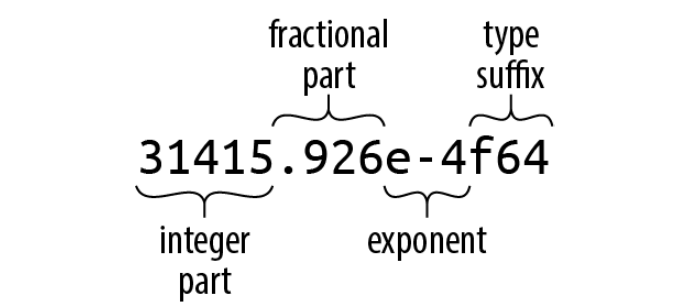
\includegraphics[width=0.8\textwidth]{../img/f3-1.png}
    \caption{浮点数字面量}
    \label{f3-1}
\end{figure}

整数部分之后的部分都是可选的，但小数部分、指数、或者类型后缀至少需要有一个，才能和整数字面量区分开。小数部分可以只有一个单独的小数点，因此\texttt{5.}是一个有效的浮点数。

如果一个浮点数字面量缺少类型后缀，和处理整数一样，Rust会检查上下文来查看这个值是如何使用的。如果最后它发现两种浮点数类型都可以满足语义，那么它会默认选择\texttt{f64}。

为了实现类型推导，Rust把整数字面量和浮点数字面量区分为不同的种类：它从来不会把一个浮点数类型推断为整数类型，反之亦然。\hyperref[t3-9]{表3-9}展示了一些浮点数字面量的例子。

\begin{table}[htbp]
    \centering
    \caption{浮点数字面量的示例}
    \label{t3-9}
    \begin{tabular}{lll}
        \hline
        \textbf{字面量} & \textbf{类型} & \textbf{数值} \\
        \hline
        \texttt{-1.5625}    & 自动推断  & $-1\frac{9}{16}$  \\
        \rowcolor{tablecolor}
        \texttt{2.}         & 自动推断  & 2 \\
        \texttt{0.25}       & 自动推断  & $\frac{1}{4}$   \\
        \rowcolor{tablecolor}
        \texttt{1e4}        & 自动推断  & 10,000    \\
        \texttt{40f32}      & \texttt{f32}  & 40    \\
        \rowcolor{tablecolor}
        \texttt{9.109\_383\_56e-31f64} & \texttt{f64} & 大约是$9.10938356\times10^{-31}$ \\
    \end{tabular}
\end{table}

\texttt{f32}和\texttt{f64}类型还关联了IEEE要求的特殊常量值例如\texttt{INFINITY}、\texttt{NEG\_INFINITY}（负无穷）、\texttt{NAN}（非数值）、\texttt{MIN}和\texttt{MAX}（最小和最大的有限值）：
\begin{minted}{Rust}
    assert!((-1. / f32::INFINITY).is_sign_negative());
    assert_eq!(-f32::MIN, f32::MAX);
\end{minted}
\texttt{f32}和\texttt{f64}类型提供了完整的数值计算的方法；例如，\texttt{2f64.sqrt()}是2的平方根。还有一些示例：
\begin{minted}{Rust}
    assert_eq!(5f32.sqrt() * 5f32.sqrt(), 5.);  // 精确的5.0
    assert_eq!((-1.01f64).floor(), -2.0);
\end{minted}

再重复一次，方法调用的优先级高于前缀运算符，因此对负数调用方法时确保要用括号括起来。

\texttt{std::f32::consts}和\texttt{std::f64::consts}模块提供了常用的数学常数，例如\texttt{E}、\texttt{PI}、2的平方根。

如果要查找浮点数的文档，记得文档里既有类型的文档，名称叫“\texttt{f32}(primitive type)”和“\texttt{f64}(primitive type)”，又有模块的文档，名称叫\texttt{std::f32}和\texttt{std::f64}。

和整数一样，在实际编码时通常你不需要写出浮点数字面量的类型后缀，但如果你要写，那么只需要指明变量和函数其中一个类型即可：
\begin{minted}{Rust}
    println!("{}", (2.0_f64).sqrt());
    println!("{}", f64::sqrt(2.0));
\end{minted}
和C和C++不同，Rust中几乎没有隐式类型转换。如果一个函数接收\texttt{f64}类型的参数，传递\texttt{i32}的值作为参数将是一个错误。事实上，Rust甚至不允许从\texttt{i16}到\texttt{i32}这样的隐式转换，即使每一个\texttt{i16}值也都是一个合法的\texttt{i32}值。但你总是可以使用\texttt{as}运算符来进行\texttt{显式}转换：\texttt{i as f64}，或者\texttt{x as i32}。

缺少隐式类型转换导致Rust的表达式可能会比C和C++中类似的表达式更加冗长。然而，隐式整数转换经常导致bug和安全漏洞。尤其是用来表示内存中某个东西的长度的整数，可能会导致意外的溢出。在我们的实践中，在Rust中显式写出类型转换可以提醒我们可能忽略的问题。

我们会在\hyperref[cast]{类型转换}一节中介绍转换的原理。

\section{布尔类型}

Rust的布尔类型\texttt{bool}只有两个值：\texttt{true}和\texttt{false}。比较运算符例如\texttt{==}和\texttt{<}会产生\texttt{bool}类型的结果：\texttt{2 < 5}的结果是\texttt{true}。

许多语言都很宽容，允许在需要布尔值的上下文中使用其他类型：C和C++隐式把字符、整数、浮点数和指针转换为布尔值，因此它们可以直接用作\texttt{if}或\texttt{while}语句的条件。Python还允许string、list、字典、甚至集合用作布尔值，如果不为空时视为true。然而Rust非常严格：像\texttt{if}和\texttt{while}这样的控制流的条件必须是\texttt{bool}表达式，短路求值运算符\texttt{\&\&}和\texttt{||}也是这样。你必须写\texttt{if x != 0 \{ ... \}}，而不能写\texttt{if x \{ ... \}}。

Rust的\texttt{as}运算符可以把\texttt{bool}值转换为整数值：
\begin{minted}{Rust}
    assert_eq!(false as i32, 0);
    assert_eq!(true  as i32, 1);
\end{minted}

然而，\texttt{as}不能反过来把整数值转换为\texttt{bool}值。你必须显式写出比较运算例如\texttt{x != 0}。

尽管\texttt{bool}类型只需要单个比特来表示，Rust还是使用整个字节来表示\texttt{bool}，因此你可以创建指向它的指针。

\section{字符}\label{char}
Rust的字符类型\texttt{char}代表一个单独的Unicode字符，是一个32位的值。

Rust使用\texttt{char}表示单个字符，但使用UTF-8编码字符串和文本流。因此，\texttt{String}表示它的文本是一个UTF-8字节序列，而不是字符的数组。

字符字面量是被单括号包围的单个字符，例如\texttt{'8'}或\texttt{'!'}。你可以使用Unicode范围内的任何字符：\texttt{'錆'}是一个\texttt{char}字面量代表日语汉字中的\emph{sabi}（rust）。\footnote{译者注：看起来这个字符可能无法正常显示，可以在源码里看到这个字符原本的样子。}

和字节字面量一样，一些字符需要反斜杠转义（\hyperref[t3-10]{表3-10}）。
\begin{table}[htbp]
    \centering
    \caption{需要反斜杠转义的字符}
    \label{t3-10}
    \begin{tabular}{lll}
        \hline
        \textbf{字符}   &   \textbf{Rust字符字面量} \\
        \hline
        单引号，\texttt{'}   &   \texttt{'\textbackslash''} \\
        \rowcolor{tablecolor}
        反斜杠，\texttt{\textbackslash} &    \texttt{'\textbackslash\textbackslash'} \\
        换行        &    \texttt{'\textbackslash n'} \\
        \rowcolor{tablecolor}
        回车        &   \texttt{'\textbackslash r'} \\
        制表符      &   \texttt{'\textbackslash t'} \\
    \end{tabular}
\end{table}

如果你喜欢的话，你可以以十六进制的方式写出一个字符的Unicode编码：
\begin{itemize}
    \item 如果字符的码点在U+0000到U+007F之间（可以据此判断是否在ASCII字符集之中），那么你可以将字符写作\texttt{'\textbackslash xHH'}，\texttt{HH}是一个两位的十六进制数字。例如，字符字面量\texttt{'*'}和\texttt{'\textbackslash x2A'}是等价的，因为字符\texttt{*}的码点是42，十六进制是2A。
    \item 你可以用\texttt{'\textbackslash u{HHHHHH}'}形式写出任何Unicode字符，\texttt{HHHHHH}是一个最长6位的十六进制数字，可以用下划线分隔。\footnote{译者注：此处原文中给了一个例子，但译者不知道该怎么打出卡纳达语里的字符，复制粘贴也不行，就省略了这个例子。}
\end{itemize}

一个\texttt{char}总是存储一个在0x0000到0xD7FF或0xE000到0x10FFFF之间的Unicode码点。一个\texttt{char}绝不会在两个范围之间（即0xD800到0xDFFF），也不会超出Unicode的编码空间（即大于0x10FFFF）。Rust使用类型系统和动态检查来确保\texttt{char}值总是在允许的范围内。

Rust永远不会进行\texttt{char}和其他任何类型之间的隐式转换。你可以使用\texttt{as}转换运算符来把\texttt{char}转换为整数类型，对于小于32位的类型，字符值的高位会被截断：\footnote{译者注：这个例子中也省略了卡纳达语字符相关的内容。}
\begin{minted}{Rust}
    assert_eq!('*' as i32, 42);
\end{minted}

另外，\texttt{u8}是唯一可以用\texttt{as}运算符转换成\texttt{char}的整数类型：Rust只会对开销很低并且不可能失败的转换使用\texttt{as}运算符，但任何\texttt{u8}之外的整数类型都包含不是有效的Unicode码点的值，因此这些转换需要运行时检查。所以，标准库提供了函数\texttt{std::char::from\_u32}接受任何\texttt{u32}值，并返回\texttt{Option<char>}：如果\texttt{u32}的值不是合法的Unicode码点，\texttt{from\_u32}会返回\texttt{None}；否则，它会返回\texttt{Some(c)}，\texttt{c}就是作为转换结果的\texttt{char}。

标准库为字符类型提供了一些有用的方法，你可以在文档中的“\texttt{char}(primitive type)”和模块“\texttt{std::char}”的页面中查找这些方法。例如：
\begin{minted}{Rust}
    assert_eq!('*'.is_alphabetic(), false);
    assert_eq!('β'.is_alphabetic(), true);
    assert_eq!('8'.to_digit(10), Some(8));
    assert_eq!(std::char::from_digit(2, 10), Some('2'));
\end{minted}

当然，单个字符显然没有字符串和文本流有趣。我们将会在\hyperref[string]{字符串类型}中介绍Rust的标准\texttt{String}类型和常用的文本处理操作。

\section{元组}
\emph{元组}是两个、或三个、四个、五个、……不同类型的值的组合。你可以将元组看作被逗号分隔和括号包围的元素序列。例如，\texttt{("Brazil", 1985)}是一个元组，它的第一个元素是一个静态分配的字符串，第二个元素是一个整数，它的类型是\texttt{(\&str, i32)}。给定一个元组值\texttt{t}，你可以通过\texttt{t.0}、\texttt{t.1}、……来访问它的元素。

某种程度上，元组类似于数组：这两个类型都代表一系列有固定顺序的值。许多编程语言合并或结合了这两种概念，但在Rust中，它们是完全独立的。一方面，元组的每个元素可以拥有不同的类型，而数组的所有元素必须有相同的类型。另外，元组只允许常数索引，例如\texttt{t.4}。你不可能写\texttt{t.i}或者\texttt{t[i]}来获取第i个元素。

Rust代码中经常使用元组类型来返回多个值。例如，字符串切片中的\texttt{split\_at}方法（用于将一个字符串切分为两半并返回）被声明为类似如下形式：
\begin{minted}{Rust}
    fn split_at(&self, mid: usize) -> (&str, &str);
\end{minted}

返回类型\texttt{(\&str, \&str)}是两个字符串切片组成的元组。你可以使用模式匹配语法来把返回的元素赋值给不同的变量：
\begin{minted}{Rust}
    let text = "I see the eigenvalue in thine eye";
    let (head, tail) = text.split_at(21);
    assert_eq!(head, "I see the eigenvalue ");
    assert_eq!(tail, "in thine eye");
\end{minted}

这比下边的等价代码可读性更强：
\begin{minted}{Rust}
    let text = "I see the eigenvalue in thine eye";
    let temp = text.split_at(21);
    let head = temp.0;
    let tail = temp.1;
    assert_eq!(head, "I see the eigenvalue ");
    assert_eq!(tail, "in thine eye");
\end{minted}

你也可以将元组视为一种极简的结构体类型。例如，在\hyperref[ch02]{第2章}的曼德勃罗集程序中，我们需要向函数传递要绘制的图片的宽度和高度。我们可以声明一个有\texttt{width}和\texttt{height}成员的结构体，但这么简单的事没有必要搞得这么复杂，因此我们用了一个元组：
\begin{minted}{Rust}
    /// 写入缓冲区`pixels`，它的大小由`bounds`给出，
    /// 写入的文件名是`filename`。
    fn write_image(filename: &str, pixels: &[u8], bounds: (usize, usize))
        -> Result<(), std::io::Error>
    { ... }
\end{minted}

参数\texttt{bounds}的类型是\texttt{(usize, usize)}，一个有两个\texttt{usize}值的元组。诚然，我们可以直接使用单独的\texttt{width}和\texttt{height}参数，生成的机器代码也会完全相同。这么写的目的只是想表明，我们把图片的大小看成一个值，而不是两个值，使用元组的写法可以清晰的表现出这一点。

元组的另一个常见用法是0元组\texttt{()}。这通常被称为\emph{单元类型}因为它只有一个取值，也写作\texttt{()}。Rust会在上下文要求某种类型，但没有有意义的值要传递的情况下使用单元类型。

例如，一个不返回值的函数的返回类型是\texttt{()}。标准库中的\texttt{std::mem::swap}函数没有有意义的返回值；它只是交换两个参数的值。\texttt{std::mem::swap}的声明如下：
\begin{minted}{Rust}
    fn swap<T>(x: &mut T, y: &mut T);
\end{minted}
\texttt{<T>}意味着\texttt{swap}是\emph{泛型}的：你可以将它用于任何类型\texttt{T}的引用。但签名中省略了\texttt{swap}的返回类型，这实际上是返回单元类型的缩写：
\begin{minted}{Rust}
    fn swap<T>(x: &mut T, y: &mut T) -> ();
\end{minted}

与此类似，我们之前提到的\texttt{write\_image}中的返回值类型是\texttt{Result<(), std::io::Error>}，这意味着如果出错时函数返回\texttt{std::io::Error}类型的值，如果成功时返回无值。

如果你想的话，你可以在元组的最后一个元素之后加上一个逗号：类型\texttt{(\&str, i32,)}和\\
\texttt{(\&str, i32)}是等价的，\texttt{("Brazil", 1985,)}和\texttt{("Brazil", 1985)}也是。Rust允许任何逗号分隔的值列表最后加上一个额外的逗号：函数参数、数组、结构体和枚举定义，等等。这对人类来说可能看起来很奇怪，但当需要在最后添加或删除条目时会变得方便一些。

为了一致性，还有只包含单个值的元组。字面量\texttt{("lonely hearts",)}是一个包含单个字符串的元组，它的类型是\texttt{(\&str,)}。这里，最后的逗号是必须的，这是为了和单纯的用括号把表达式括起来相区分。

\section{指针类型}
Rust有几个表示内存地址的类型。

这是Rust和其他大多数有垃圾回收语言的不同之处。在Java中，如果\texttt{class Rectangle}包含一个字段\texttt{Vector2D upperLeft}，那么\texttt{upperLeft}实际上是对另一个单独创建的\texttt{Vector2D}对象的引用。在Java中一个对象从来不会真的包含其他对象。

Rust里则不同。Rust被设计为尽量减少内存分配。默认情况下Rust里是值嵌套的，值\texttt{((0, 0), (1440, 900))}被存储为四个相邻的整数。如果你把它赋值给一个局部变量，那么你将得到一个4个整数大小的局部变量，不会在堆上分配任何内存。

这有助于提高内存效率，但它会导致当Rust程序需要指向其他值的指针时，必须显式使用指针类型。好消息是safe Rust里的指针类型有一些约束来保证不会出现未定义行为，因此Rust中的指针比C++中的更容易正确使用得多。

我们将会在这里讨论三种指针类型：引用、box、unsafe指针。

\subsection{引用}

一个\texttt{\&String}（读作“ref String”）类型的值是一个\texttt{String}值的引用，一个\texttt{\&i32}类型的值是一个\texttt{i32}值的引用，等等。

把引用想象成Rust的基本指针类型可以让我们更容易理解。在运行时，一个\texttt{i32}的引用是一个单独的机器字，里面存储的是指向的\texttt{i32}值的地址，可能在栈上也可能在堆上。表达式\texttt{\&x}产生一个\texttt{x}的引用；在Rust的术语中，我们称它\emph{借用了\texttt{x}的引用}。给定引用\texttt{r}，表达式\texttt{*r}就是\texttt{r}指向的值。这些类似于C和C++中的\texttt{\&}和\texttt{*}运算符。和C指针类似，当引用离开作用域时并不会自动释放任何资源。

然而和C指针不同的是，Rust的引用永远不为空：在safe Rust中没有任何办法产生一个空引用。而且和C指针不同，Rust通过追踪值的所有权和生命周期，在编译期就可以杜绝悬垂指针、double free和指针失效的情况。

Rust的指针有以下两种类型：

\codeentry{\&T}
\hangparagraph{一个不可变的共享引用。你可以同时拥有同一个值的多个共享的引用，但它们都是只读的：修改它们指向的值是禁止的，就像C中的\texttt{const T*}一样。}

\codeentry{\&mut T}
\hangparagraph{一个可变的、独占的引用。你可以读写它指向的值，类似于C中的\texttt{T*}。但只要这个引用存在，你不能再持有任何这个值的其他任何类型的引用。事实上，这时候你唯一可以访问这个值的方法就是通过这个可变引用。}

Rust使用这种方式来区分共享和可变的引用，以此来强制执行“单个写者或多个读者”规则：要么你可以读写值，要么它只能被任何数量的读者共享。这种分隔由编译器检查来强制执行，它是Rust安全保证的核心。\hyperref[ch05]{第5章}解释了Rust中使用安全引用的规则。

\subsection{\texttt{Box}}

最简单的在堆上分配内存的方式是使用\texttt{Box::new}：
\begin{minted}{Rust}
    let t = (12, "eggs");
    let b = Box::new(t);    // 在堆上分配一个元组
\end{minted}

\texttt{t}的类型是\texttt{(i32, \&str)}，因此\texttt{b}的类型是\texttt{Box<(i32, \&str)>}。调用\texttt{Box::new}会在堆上分配足够的内存来存储元组。当\texttt{b}离开作用域时，内存会被立即释放，除非\texttt{b}被\texttt{move}了——例如被返回了。move对Rust处理堆上分配的值的方式至关重要，我们将在\hyperref[ch04]{第4章}详解介绍这一点。

\subsection{原始指针}

Rust也有原始指针类型\texttt{*mut T}和\texttt{*const T}。原始指针类似于C++中的指针。使用原始指针是不安全的，因为Rust无法追踪它指向的到底是什么。例如，原始指针可能是空、或者可能指向被释放的内存、或者现在指向一个和之前不同类型的值。所有C++中经典的指针错误都有可能。

然而，你只能在\texttt{unsafe}块中解引用原始指针。\texttt{unsafe}块是Rust中的可选机制，它的安全性取决于你自己。如果你的代码没有\texttt{unsafe}块（或者有\texttt{unsafe}块但里面的代码都是完全正确的），那么整本书中强调的安全性保证都适用。细节见\hyperref[ch22]{第22章}。

\section{数组、vector和切片}
Rust有三种表示一系列值的类型：
\begin{itemize}
    \item 类型\texttt{[T; N]}表示一个有\texttt{N}个元素的数组，每个元素的类型都是\texttt{T}。每个数组的长度必须在编译期已知，并且是类型的一部分。你不能添加新元素或者缩减元素。
    \item 类型\texttt{Vec<T>}，是类型\texttt{T}的向量。它是动态分配、可增长的类型\texttt{T}的值的序列。vector的元素存储在堆中，所以你可以按需更改vector的大小：可以添加新的元素、附加其它vector、删除元素等。
    \item 类型\texttt{\&[T]}和\texttt{\&mut [T]}分别是类型\texttt{T}的共享切片和可变切片，它们是数组或vector等其它值中的一部分元素的引用。你可以把切片当做一个指向第一个元素的指针再加上一个可访问的元素数量。一个可变的切片\texttt{\&mut [T]}让你可以读取并修改元素，但不能被共享；共享的切片\texttt{\&[T]}允许你在多个读者间共享数据，但不能修改元素。
\end{itemize}

如果\texttt{v}是这三种类型中的任意一种，那么表达式\texttt{v.len()}返回\texttt{v}中元素的数量，\texttt{v[i]}返回\texttt{v}中的第\texttt{i+1}个元素。第一个元素是\texttt{v[0]}，最后一个元素是\texttt{v[v.len() - 1]}。Rust会检查\texttt{i}是否在范围内，如果超过了长度范围，表达式会panic。\texttt{v}的长度可能是0，这时任何索引操作都会panic。\texttt{i}必须是\texttt{usize}类型的值，你不能使用任何其它整数类型当作索引。

\subsection{数组}
创建一个数组有几种方式。最简单的方式是用方括号括起来的一系列值：
\begin{minted}{Rust}
    let lazy_caterer: [u32; 6] = [1, 2, 4, 7, 11, 16];
    let taxonomy = ["Animalia", "Arthropoda", "Insecta"];

    assert_eq!(lazy_caterer[3], 7);
    assert_eq!(taxonomy.len(), 3);
\end{minted}

如果想要初始化定长数组，可以使用\texttt{[V; N]}的写法，其中\texttt{V}是每一个元素的初始值，\texttt{N}是长度。例如，\texttt{[true; 10000]}代表含有10,000个\texttt{bool}类型元素的数组，每个元素都被初始化为\texttt{true}：
\begin{minted}{Rust}
    let mut sieve = [true; 10000];
    for i in 2..100 {
        if sieve[i] {
            let mut j = i * i;
            while j < 10000 {
                sieve[j] = false;
                j += i;
            }
        }
    }

    assert!(sieve[211]);
    assert!(!sieve[9876]);
\end{minted}

你会发现这种语法还可以用于创建固定大小的缓冲区：\texttt{[0u8; 1024]}可以用作一个1K的缓冲区，所有字节全部初始化为0。Rust里没有创建未初始化数组的语法。（更广泛的说，Rust保证代码不可能访问任何未初始化的值。）

一个数组的长度是类型的一部分，并且在编译期就已经固定。如果\texttt{n}是一个变量，你不能用\texttt{[true; n]}这种语法来得到一个有\texttt{n}个元素的数组。当你需要运行时才能确定长度的数组时，使用vector来代替。

数组有一些有用的方法——迭代元素、搜索、排序、填充、过滤等等——事实上这些方法都是切片的，而不是数组的。但在搜索方法时Rust会隐式的把数组的引用转换为切片，因此你可以直接用数组调用切片的方法：
\begin{minted}{Rust}
    let mut chaos = [3, 5, 4, 1, 2];
    chaos.sort();
    assert_eq!(chaos, [1, 2, 3, 4, 5]);
\end{minted}

这里，\texttt{sort}方法实际上是为切片定义的，但因为它是以调用者的引用为参数，所以Rust隐式的创建了一个引用整个数组的\texttt{\&mut [i32]}类型的切片，然后在这个切片上调用\texttt{sort}方法。事实上，我们之前提到的\texttt{len}方法最早的时候也是切片的方法。我们将在\hyperref[slice]{切片}这一节中介绍切片。

\subsection{vector}\label{vector}

一个\texttt{Vec<T>}是一个长度可变的类型\texttt{T}的数组，它的元素都存储在堆上。

有几种创建vector的方法。最简单的方法是使用\texttt{vec!}宏，这种语法很像数组字面量：
\begin{minted}{Rust}
    let mut primes = vec![2, 3, 5, 7];
    assert_eq!(primes.iter().product::<i32>(), 210);
\end{minted}
当然，这是vector，不是数组，因此我们可以动态添加元素：
\begin{minted}{Rust}
    primes.push(11);
    primes.push(13);
    assert_eq!(primes.iter().product::<i32>(), 30030);
\end{minted}

你也可以再次使用类似于数组字面量的语法来创建重复给定值若干次的vector：
\begin{minted}{Rust}
    fn new_pixel_buffer(rows: usize, cols: usize) -> Vec<u8> {
        vec![0; rows * cols]
    }
\end{minted}
\texttt{vec!}宏等价于调用\texttt{Vec::new}创建一个新的空vector，然后向其中添加元素：
\begin{minted}{Rust}
    let mut pal = Vec::new();
    pal.push("step");
    pal.push("on");
    pal.push("no");
    pal.push("pets");
    assert_eq!(pal, vec!["step", "on", "no", "pets]);
\end{minted}

另一种创建vector的方法是通过迭代器创建：
\begin{minted}{Rust}
    let v: Vec<i32> = (0..5).collect();
    assert_eq!(v, [0, 1, 2, 3, 4]);
\end{minted}

通常使用\texttt{collect}时你需要给出类型，因为它可以生成不同类型的集合，不只是vector。但指明了\texttt{v}的类型之后，我们需要的集合类型就没有歧义了。

类似于数组，你也可以对vector调用切片的方法：
\begin{minted}{Rust}
    // 回文
    let mut palindrome = vec!["a man", "a plan", "a canal", "panama"];
    palindrome.reverse();
    // 合理但令人失望
    assert_eq!(palindrome, vec!["panama", "a canal", "a plan", "a man"]);
\end{minted}

这里，\texttt{reverse}方法实际上是为切片定义的，但这里调用隐式地借用了vector的\texttt{\&mut [\&str]}切片，然后对它调用了\texttt{reverse}。

\texttt{Vec}是Rust中不可或缺的一个类型——它被用在几乎所有需要动态大小列表的场景——所以有很多其他的方法创建构造新的vector或扩展现有的列表，我们将在\hyperref[ch16]{第16章}介绍它们。

一个\texttt{Vec<T>}由3个值组成：一个指针指向堆上存储元素的缓冲区，这个缓冲区的所有权属于这个\texttt{Vec<T>}；缓冲区可以存储的元素的数量；它现在实际已经拥有的元素的数量（也就是它的长度）。当缓冲区的的元素到达最大容量时，继续添加元素会导致vector重新分配一个更大的缓冲区，再把已有元素都拷贝过去，然后更新vector的指针和容量，最后释放旧的缓冲区。

如果你提前知道vector需要存储的元素的数量，你可以使用\texttt{Vec::with\_capacity}来创建一个从一开始就拥有足以存下它们的缓冲区的vector；然后你可以向vector中添加元素，并且不会导致重新分配内存。\texttt{vec!}宏就使用了类似这样的方法，因为它知道最终的vector会有多少个元素。注意这只决定了vector的初始大小，如果你继续添加元素，vector会像通常一样变大。

很多库函数都在寻找使用\texttt{Vec::with\_capacity}代替\texttt{Vec::new}的机会。例如，在\texttt{collect}的例子中，迭代器\texttt{0..5}提前知道它会产生5个值，\texttt{collect}函数就可以利用这一点提前分配足够容量的vector。我们将在\hyperref[ch15]{第15章}中介绍这些。

就像\texttt{len}方法会返回持有的元素数量一样，它的\texttt{capacity}方法会返回它在不重新分配的前提下能存储的最大元素数量：
\begin{minted}{Rust}
    let mut v = Vec::with_capacity(2);
    assert_eq!(v.len(), 0);
    assert_eq!(v.capacity(), 2);

    v.push(1);
    v.push(2);
    assert_eq!(v.len(), 2);
    assert_eq!(v.capacity(), 2);

    v.push(3);
    assert_eq!(v.len(), 3);
    // 通常会打印出 "capacity is now 4":
    println!("capacity is now {}", v.capacity());
\end{minted}

最后打印出的容量并不保证是4，但通常至少是3，因为vector已经持有3个元素了。

你可以在vector中任意插入或移除元素，尽管这些操作会移动修改位置前面或者后面的元素，因此如果vector很长的时候这些操作会很慢：
\begin{minted}{Rust}
    let mut v = vec![10, 20, 30, 40, 50];

    // 在索引为3的地方插入35
    v.insert(3, 35);
    assert_eq!(v, [10, 20, 30, 35, 40, 50]);

    // 移除索引为1的元素
    v.remove(1);
    assert_eq!(v, [10, 30, 35, 40, 50]);
\end{minted}

你可以使用\texttt{pop}方法移除最后一个元素并返回它。更确切地说，从\texttt{Vec<T>}中弹出只会返回一个\texttt{Option<T>}：如果vector已经为空是\texttt{None}，如果最后一个元素是\texttt{v}就是\texttt{Some(v)}：
\begin{minted}{Rust}
    let mut v = vec!["Snow Puff", "Glass Gem"];
    assert_eq!(v.pop(), Some("Glass Gem"));
    assert_eq!(v.pop(), Some("Snow Puff));
    assert_eq!(v.pop(), None);
\end{minted}

你可以使用\texttt{for}循环来迭代vector：
\begin{minted}{Rust}
    // 把命令行参数收集为String的vector
    let languages: Vec<String> = std::env::args().skip(1).collect();
    for l in languages {
        println!("{}: {}", l,
            if l.len() % 2 == 0 {
                "functional"
            } else {
                "imperative"
            });
    }
\end{minted}

用一些编程语言的名字来运行这个程序，你就会发现有趣的地方：
\begin{minted}{text}
    $ cargo run Lisp Scheme C C++ Fortran
       Compiling proglangs v0.1.0 (/home/jimb/rust/proglangs)
        Finished dev [unoptimized + debuginfo] target(s) in 0.36s
         Running `target/debug/proglangs Lisp Scheme C C++ Fortran`
    Lisp: functional
    Scheme: functional
    C: imperative
    C++: imperative
    Fortran: imperative
\end{minted}

终于，我们得到了术语\emph{函数式语言}的一个令人满意的定义。\footnote{译者注：此处作者应该是开玩笑。}

尽管\texttt{Vec}非常重要，但它只是Rust中定义的一个普通类型，不是语言内建的类型。我们将在\hyperref[ch22]{第22章}中介绍实现这样的类型的技术。

\subsection{切片}\label{slice}

一个切片写作\texttt{[T]}，没有长度。它表示数组或vector的一部分。因为切片可以是任意长度，因此切片不能直接存储在变量中或者作为参数传递。切片必须通过引用传递。

切片的引用是\emph{胖指针}：一个包含指向切片中第一个元素的指针和切片中元素数量的双字值。

假设你正在运行下列代码：
\begin{minted}{Rust}
    let v: Vec<f64> = vec![0.0,  0.707,  1.0,  0.707];
    let a: [f64; 4] =     [0.0, -0.707, -1.0, -0.707];

    let sv: &[f64] = &v;
    let sa: &[f64] = &a;
\end{minted}

在最后两行中，Rust自动把\texttt{\&Vec<f64>}和\texttt{\&[f64; 4]}转换成了切片的引用。

这段代码运行完后，内存布局类似\hyperref[f3-2]{图3-2}中所示：
\begin{figure}[htbp]
    \centering
    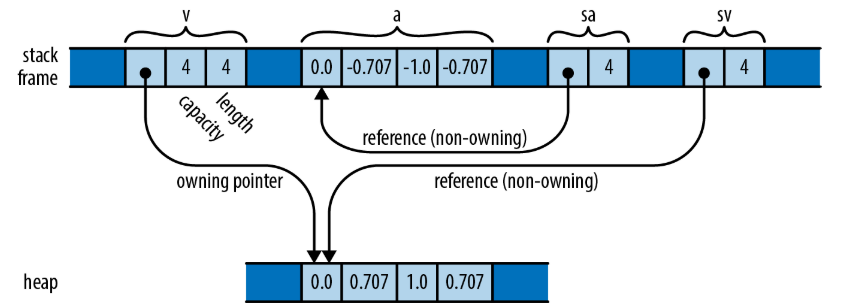
\includegraphics[width=0.9\textwidth]{../img/f3-2.png}
    \caption{一个vector \texttt{v}和一个数组\texttt{a}，以及分别指向它们的切片\texttt{sv}和\texttt{sa}的内存布局}
    \label{f3-2}
\end{figure}

一个普通的引用是一个指向单个值的无所有权指针，而一个切片的引用是一个指向内存中连续的范围的指针。这使得如果你想写一个处理数组或vector的函数，那么切片引用将是一个很好的选择。例如，这里有一个函数打印出一系列值，每个单独一行：
\begin{minted}{Rust}
    fn print(n: &[f64]) {
        for elt in n {
            println!("{}", elt);
        }
    }

    print(&a);  // 可以用于数组
    print(&v);  // 可以用于vector
\end{minted}

因为这个函数的参数是切片引用，你可以像示例中一样传递数组或者vector的引用。事实上，很多你可能以为是数组或vector的方法实际上都是切片的方法：例如\texttt{sort}和\texttt{reverse}方法，实际上都是切片类型\texttt{[T]}的方法。

你可以通过索引一个数组或vector或一个现有切片的一个范围来得到一个切片引用：
\begin{minted}{Rust}
    print(&v[0..2]);    // 打印出v的前两个元素
    print(&a[2..]);     // 打印出从a[2]开始剩余的元素
    print(&sv[1..3]);   // 打印出v[1]和v[2]
\end{minted}

类似于普通的数组访问，Rust会检查索引的有效性。尝试借用超过数据结尾的切片会导致panic。

因为切片类型总是以引用的方式出现，我们也经常用“切片”来指代\texttt{\&[T]}或\texttt{\&str}这样的类型，用最短的名称表达最常用的概念。

\section{字符串类型}\label{string}

熟悉C++的程序员应该都知道C++里有两种字符串类型：字符串字面量的类型\texttt{const char *}，标准库里还提供了一个类\texttt{std::string}，用于在运行时动态创建字符串。

Rust的设计与此类似。在这一节中，我们将首先展示字符串字面量的所有写法，然后介绍Rust的两种字符串类型。我们将在\hyperref[ch17]{第17章}中详细讨论字符串和文本的处理。

\subsection{字符串字面量}\label{StrLiteral}

字符串字面量被双引号包裹，和\texttt{char}字面量一样是通过反斜杠来转义：
\begin{minted}{Rust}
    let speech = "\"Ouch!\" said the well.\n";
\end{minted}

在字符串字面量里和\texttt{char}字面量里不同的一点是，单引号不需要使用反斜杠转义，但双引号需要。

一个字符串可以占多行：
\begin{minted}{Rust}
    println!("In the room the women come and go,
        Singing of Mount Abora");
\end{minted}
这个字符串里的换行符被包括在字符串里，因此也会被输出。第二行开头的空格也是。


如果字符串中的一行以反斜杠结尾，那么换行符和下一行的前导空格就会被丢弃掉：
\begin{minted}{Rust}
    println!("It was a bright, cold day in April, and \
        there were four of us-\
        more or less.");
\end{minted}
这段代码会打印出单行文本。打印出的字符串里“and”和“there”之间有一个空格，因为第一行的反斜杠前边有一个空格，而连字符和“more”之间没有空格。

在少数情况下，在字符串里用反斜杠转义反斜杠是一件很烦的事情。（典型的例子就是正则表达式和Windows的路径）对于这种情况，Rust提供了\emph{原始字符串}，原始字符串用小写字母\texttt{r}来标记。原始字符串中的所有反斜杠和空白字符都被原样包含在字符串里，不会识别任何转义：
\begin{minted}{Rust}
    let default_win_install_path = r"C:\Program Files\Gorillas";

    let pattern = Regex::new(r"\d+(\.\d+)*");
\end{minted}

你不能通过在前面加上反斜杠来把双引号包含在原始字符串中——记住，我们说的是\emph{不会识别任何转义}。然而，这种情况也有解决的方法。原始字符串的开头和结尾可以用任意相同数量的井号来标记：
\begin{minted}{Rust}
    println!(r###"
        This raw string started with 'r###"'.
        Therefore it does not end until we reach a quote mark ('"')
        followed immediately by three pound signs ('###'):
    "###);
\end{minted}

您可以根据需要添加井号，以明确原始字符串的结束位置。

\subsection{字节字符串}

以\texttt{b}前缀开头的字符串字面量是\emph{字节字符串}。这种字符串实际上是\texttt{u8}值的切片——也就是字节流——而不是Unicode文本：
\begin{minted}{Rust}
    let method = b"GET";
    assert_eq!(method, &[b'G', b'E', b'T']);
\end{minted}

\texttt{method}的类型是\texttt{\&[u8; 3]}：它是一个有三个字节的数组的引用。它没有任何我们之后要讨论的字符串的方法。它和字符串最像的地方就是我们创建它时用的语法。

字节字符串可以使用我们之前使用过的所有语法：它也可以跨多行、使用反斜杠转义、使用反斜杠连接多行。还有以\texttt{br"}开头的原始字节字符串。

字节字符串不能包含任意Unicode字符，它只能包含ASCII和用\texttt{\textbackslash xHH}形式表示的字符。

\subsection{内存中的字符串}

Rust的字符串是Unicode字符的序列，但它并不是作为\texttt{char}的数组存储在内存中。事实上它使用UTF-8编码存储，这是一种可变长度的编码。每一个ASCII字符被存储为一个字节，其他字符可能会占据多个字节。

\hyperref[f3-3]{图3-3}显示了下面代码创建的\texttt{String}和\texttt{\&str}：\footnote{译者注：因为不知道怎么打出来这些卡纳达语字符，所以用“某些卡纳达语字符”代替。}
\begin{minted}{Rust}
    let noodles = "noodles".to_string();
    let oodles = &noodles[1..];
    let poodles = "某些卡纳达语字符";
\end{minted}

\begin{figure}[htbp]
    \centering
    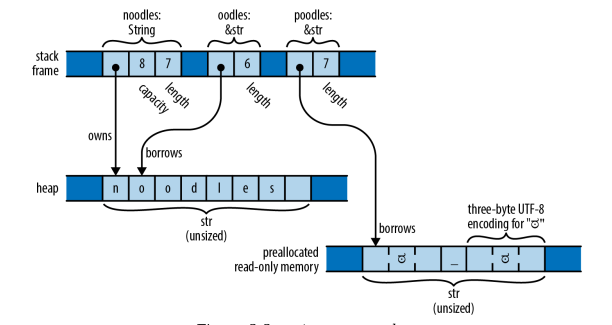
\includegraphics[width=0.8\textwidth]{../img/f3-3.png}
    \caption{\texttt{String, \&str, str}}
    \label{f3-3}
\end{figure}

一个\texttt{String}有一个大小可变的缓冲区来存储UTF-8文本。缓冲区是在堆上分配的，所以它可以按需或按照要求调整缓冲区大小。在这个例子中，\texttt{noodles}是一个拥有8个字节大小的缓冲区的\texttt{String}，其中7个字节已经被使用。你可以将\texttt{String}想象为保证内容是有效UTF-8编码的\texttt{Vec<u8>}；事实上，\texttt{String}就是这么实现的。

一个\texttt{\&str}（读作“stir”或者“字符串切片”）是一个指向其他值拥有的UTF-8文本的引用：它“借用”了这段文本。在这个例子中，\texttt{oodles}是一个指向\texttt{noodles}所持有的文本中的最后六个字节的\texttt{\&str}，因此它表示文本“oodles”。就像其他切片引用一样，\texttt{\&str}是一种胖指针，包括实际数据的地址和长度。你可以将\texttt{\&str}看作一个保证内容为合法的UTF-8编码的\texttt{\&[u8]}。

字符串字面量是一个指向预先分配好内存的文本的\texttt{\&str}，实际的文本通常和程序的机器码一起存储到只读的内存区域。在之前的例子中，\texttt{poodles}是一个字符串字面量，指向程序运行时就已经被创建好并且持续到程序退出的7个字节。

一个\texttt{String}或\texttt{\&str}的\texttt{len()}方法返回它的长度。但这个长度是以字节为单位，而不是以字符为单位：
\begin{minted}{Rust}
    assert_eq!("某些卡纳达语字符".len(), 24);
    assert_eq!("某些卡纳达语字符".chars().count(), 8);
\end{minted}

不能修改\texttt{\&str}：
\begin{minted}{Rust}
    let mut s = "hello";
    s[0] = 'c';     // error: `&str`不能被修改，以及其他原因
    s.push('\n');   // error: `&str`没有`push`方法
\end{minted}

要在运行时创建新的字符串，要使用\texttt{String}。

类型\texttt{\&mut str}确实存在，但它并不好用，因为几乎所有对UTF-8的操作都可能改变字节长度，而一个切片不能重新分配它指向的参照物。事实上，\texttt{\&mut str}唯一能做的操作是\texttt{make\_ascii\_uppercase}和\texttt{make\_ascii\_lowercase}，这两个操作在原址修改文本，并且只影响单个字节的字符。

\subsection{\texttt{String}}
\texttt{\&str}和\texttt{\&[T]}很像：都是一个指向某些数据的胖指针。\texttt{String}类似于\texttt{Vec<T>}，如\hyperref[t3-11]{表3-11}所示。

\begin{table}[htbp]
    \centering
    \caption{\texttt{Vec<T>}和\texttt{String}的比较}
    \label{t3-11}
    \begin{tabular}{p{0.6\textwidth}p{0.15\textwidth}p{0.15\textwidth}}
        \hline
                    & \textbf{\texttt{Vec<T>}} & \textbf{\texttt{String}} \\
        \hline
        自动释放缓冲区 & 是 & 是 \\
        \rowcolor{tablecolor}
        可增长       & 是 & 是 \\
        有\texttt{::new()}和\texttt{::with\_capacity()}类型关联函数 & 是 & 是 \\
        \rowcolor{tablecolor}
        \texttt{.reserve()}和\texttt{.capacity()}方法 & 是 & 是 \\
        \texttt{.push()}和\texttt{.pop()}方法 & 是 & 是 \\
        \rowcolor{tablecolor}
        范围语法\texttt{v[start..stop]} & 是，返回\texttt{\&[T]} & 是，返回\texttt{\&str} \\
        自动转换      & \texttt{\&Vec<T>}到\texttt{\&[T]} & \texttt{\&String}到\texttt{\&str} \\
        \rowcolor{tablecolor}
        继承方法      & 从\texttt{\&[T]} & 从\texttt{\&str} \\
    \end{tabular}
\end{table}

类似于\texttt{Vec}，每个\texttt{String}都有它自己的在堆上分配的缓冲区，这个缓冲区不和其他任何\texttt{String}共享。当一个\texttt{String}变量离开作用域时，缓冲区会自动释放，除非\texttt{String}被move了。

有几种方式创建\texttt{String}：
\begin{itemize}
    \item \texttt{.to\_string()}方法把\texttt{\&str}转换为一个\texttt{String}，这会拷贝字符串：
    \begin{minted}{Rust}
    let error_message = "too many pets".to_string();
    \end{minted}
    \texttt{.to\_owned()}方法做同样的事，你可能会看到它用同样的方式使用。它也可以用于其他类型，正如我们将在\hyperref[ch13]{第13章}讨论的一样。

    \item \texttt{format!()}宏类似于\texttt{println!()}，区别在于它返回一个新的\texttt{String}而不是把它打印到标准输出，而且它不会在最后自动加上换行符：
    \begin{minted}{Rust}
    assert_eq!(format!("{}°{:02}′{:02}″N", 24, 5, 23),
               "24°05′23″N".to_string());
    \end{minted}

    \item 字符串的数组、切片、vector都有两个方法\texttt{.concat()}和\texttt{.join(sep)}，把多个字符串组合成一个：
    \begin{minted}{Rust}
    let bits = vec!["veni", "vidi", "vici"];
    assert_eq!(bits.concat(), "venividivici");
    assert_eq!(bits.join(", "), "veni, vidi, vici");
    \end{minted}
\end{itemize}

有时你需要选择使用\texttt{\&str}还是\texttt{String}。\hyperref[ch05]{第5章}将详细介绍这个问题。现在你只需要知道\texttt{\&str}可以指向任何字符串的任何切片，不管是字符串字面量（存储在可执行文件中）还是\texttt{String}（在运行时分配和释放）。这意味着当允许调用者传递任何类型的字符串时\texttt{\&str}更适合用作参数的类型。

\subsection{使用字符串}

字符串支持\texttt{==}和\texttt{!=}运算符。只有当两个字符串含有内容和顺序都完全相同的字符时两个字符串才相等（和它们在内存中的位置无关）：
\begin{minted}{Rust}
    assert!("ONE".to_lowercase() == "one");
\end{minted}

字符串还支持比较运算符\texttt{<, <=, >, >=}，以及很多你可以在在线文档的“\texttt{str}(primitive type)”或“\texttt{std::str}”模块的页面中找到的有用的方法和函数（或者直接跳转到\hyperref[ch17]{第17章}）。这里有一些例子：
\begin{minted}{Rust}
    assert!("peanut".contains("nut"));
    assert_eq!("    clean\n".trim(), "clean");

    for word in "veni, vidi, vici".split(", ") {
        assert!(word.starts_with("v"));
    }
\end{minted}

注意，因为Unicode的特性，简单的逐字符比较\emph{并不}总是能给出预期的答案。例如，字符串\texttt{"th\textbackslash{}u\{e9\}"}和\texttt{"the\textbackslash{}u\{301\}"}都是有效的\textbf{thé}（法语中表示茶的单词）的Unicode表示。Unicode认为它们应该以相同的方式展示和处理，但是Rust把它们当作两个完全不同的字符串。类似的，Rust的比较运算符例如\texttt{<}只是简单的使用基于字符码点值的字典顺序。这种顺序只是偶尔和用户语言和文化中用于文本的排序一致。我们将在\hyperref[ch17]{第17章}中详细讨论这个问题。

\subsection{其他类似字符串的类型}

Rust保证字符串是有效的UTF-8字符串。有时一个程序可能会需要处理\emph{非}有效的Unicode字符串。这通常发生在Rust程序与其他不强制遵循Unicode的系统交互时。例如，在大多数操作系统中很容易就能创建一个文件名不是有效的Unicode的文件。当Rust遇到这样的文件名时该如何处理？

Rust的方法是为这些场景提供一些类似字符串的类型：
\begin{itemize}
    \item 对于Unicode文本坚持使用\texttt{String}和\texttt{\&str}。
    \item 当处理文件名时，使用\texttt{std::path::PathBuf}和\texttt{\&Path}来代替。
    \item 当处理完全不是UTF-8编码的二进制数据时，使用\texttt{Vec<u8>}和\texttt{\&[u8]}。
    \item 当处理环境变量名称或者命令行参数这些由操作系统提供的内容时，使用\texttt{OsString}和\\\texttt{\&OsStr}。
    \item 当和以空字符结尾的C库交互时，使用\texttt{std::ffi::CString}和\texttt{\&CStr}。
\end{itemize}

\section{类型别名}

\texttt{type}关键字可以像C++中的\texttt{typedef}一样为已存在的类型声明一个新名字：
\begin{minted}{Rust}
    type Bytes = Vec<u8>;
\end{minted}

我们在这里声明的\texttt{Bytes}就是这种特定类型的\texttt{Vec}：
\begin{minted}{Rust}
    fn decode(data: &Bytes) {
        ...
    }
\end{minted}

\section{基本类型之外}

类型是Rust的一个核心部分。我们将在整本书中继续讨论类型并介绍新的类型。特别是，Rust的用户自定义类型赋予了语言很多自身的风格。有三种用户自定义的类型，我们将分别在三章中介绍它们：\hyperref[ch09]{第9章}介绍结构体，\hyperref[ch10]{第10章}介绍枚举，\hyperref[ch11]{第11章}介绍trait。

函数和闭包有它们自己的类型，这将在\hyperref[ch14]{第14章}中介绍。标准库中的类型将在整本书中介绍。例如，\hyperref[ch16]{第16章}介绍标准集合类型。

不过，这些都还需要等一会。在我们继续之前，是时候了解一下Rust安全规则的核心概念了。

\chapter{所有权与move}\label{ch04}
\chapter{引用}\label{ch05}

\emph{Libraries cannot provide new inabilities.}

\begin{flushright}
——Mark Miller
\end{flushright}

我们至今为止见过的所有指针类型——简单的\texttt{Box<T>}堆指针、\texttt{String}和\texttt{Vec}内部的指针都拥有值：当所有者被drop时，指针指向的值也会随之消失。Rust还有非拥有指针类型，称为\emph{引用}，引用对指向的值的生命周期没有影响。

事实上，正相反，引用绝不应该比它们指向的值活的更长。你必须在你的代码中明确表明，引用的生命寿命比它指向的值更短。为了强调这一点，Rust将创建某个值的引用称为\emph{借用}值：你最终必须把你借走的还给它的所有者。

如果你在读到“你必须在你的代码中明确表明”时感到一丝怀疑，那说明你很优秀。引用自身并没有什么特殊的——本质上，它们只是地址。但保证它们安全的规则是Rust独有的，你以前不可能看到过类似的。尽管这些规则是Rust里最难掌握的部分，但它们能防止的经典的、日常的bug的范围之广令人惊讶，它们对多线程的影响也正在显现。这也是Rust的赌注。

这一章中，我们将讨论Rust中的引用如何工作，展示引用、函数和自定义类型如何包含生命周期信息来保证它们被安全使用，阐释它怎么能在编译期、不引入运行时开销的同时防止常见的bug。

\section{值的引用}

举个例子，假设我们要为文艺复兴时期优秀的艺术家和他们的著名作品建一个表格。Rust的标准库包含一个哈希表类型，所以我们可以像这样定义我们的类型：
\begin{minted}{Rust}
    use std::collections::HashMap;

    type Table = HashMap<String, Vec<String>>;
\end{minted}

换句话说，这是一个把\texttt{String}值映射到\texttt{Vec<String>}值的哈希表，它把艺术家的名字关联到它们的作品的名字。你可以使用\texttt{for}循环来迭代\texttt{HashMap}的条目，因此我们可以写一个函数打印出一个\texttt{Table}：
\begin{minted}{Rust}
    fn show(table: Table) {
        for (artist, works) in table {
            println!("works by {}:", artist);
            for work in works {
                println!("  {}", work);
            }
        }
    }
\end{minted}

构造和打印表格都很直观：
\begin{minted}{Rust}
    fn main() {
        let mut table = Table::new();
        table.insert("Gesualdo".to_string(),
                     vec!["many madrigals".to_string(),
                          "Tenebrae Responsoria".to_string()]);
        table.insert("Caravaggio".to_string(),
                     vec!["The Musicians".to_string(),
                          "The Calling of St. Matthew".to_string()]);
        table.insert("Cellini".to_string(),
                     vec!["Perseus with the head of Medusa".to_string(),
                          "a salt cellar".to_string()]);
        show(table);
    }
\end{minted}

它也能正常工作：
\begin{minted}{text}
    $ cargo run
         Running `/home/jimb/rust/book/fragments/target/debug/fragments`
    works by Gesualdo:
      many madrigals
      Tenebrae Responsoria
    works by Cellini:
      Perseus with the head of Medusa
      a salt cellar
    works by Caravaggio:
      The Musicians
      The Calling of St. Matthew
\end{minted}

但如果你阅读过上一章中有关move的小节，你就会发现\texttt{show}的定义有一些问题。首先，\texttt{HashMap}不是\texttt{Copy}类型——它不可能是，因为它持有动态分配的表格。因此当程序调用\texttt{show(table)}时，整个结构都被移动到函数里，变量\texttt{table}将变为未初始化。（迭代它时没有特定的顺序，你可能会得到一个不同的顺序，不用担心）如果调用者代码尝试继续使用\texttt{table}，它会遇到问题：
\begin{minted}{Rust}
    ...
    show(table);
    assert_eq!(table["Gesualdo"][0], "many madrigals");
\end{minted}

Rust会报错\texttt{table}不再可用：
\begin{minted}{text}
    error: borrow of moved value: `table`
       |
    20 |     let mut table = Table::new();
       |         --------- move occurs because `table` has type
       |                   `HashMap<String, Vec<String>>`,
       |                   which does not implement the `Copy` trait
    ...
    31 |     show(table);
       |          ----- value moved here
    32 |     assert_eq!(table["Gesualdo"][0], "many madrigals");
       |                ^^^^^ value borrowed here after move
\end{minted}

事实上，如果我们仔细查看\texttt{show}的定义，会发现外层的\texttt{for}循环获取了哈希表的所有权然后完全消费了它，内层的\texttt{for}循环对每一个vector做了同样的事（我们之前已经在“liberté, égalité, fraternité”的例子中见过这种行为了）。因为move语义，我们仅仅是为了打印它就已经完全销毁了整个结构体。感谢你，Rust！

正确的处理方式是使用引用。引用让你可以访问一个值，同时不影响它的所有权。引用有两种：
\begin{itemize}
    \item \emph{共享引用}让你能读取但不能修改被引用的值。然而，你可以同时持有多个共享引用。表达式\texttt{\&e}返回一个指向\texttt{e}的值的共享引用，如果\texttt{e}的类型是\texttt{T}，那么\texttt{\&e}的类型就是\texttt{\&T}，读作“ref \texttt{T}”。共享引用是\texttt{Copy}类型。
    \item 如果你有一个值的\emph{可变引用}，你可以读取和修改这个值。然而，你不能同时再有任何其他有效的引用。表达式\texttt{\&mut e}返回一个指向\texttt{e}的值的可变引用，它的类型是\texttt{\&mut T}，读作“ref mute \texttt{T}”。可变引用不是\texttt{Copy}类型。
\end{itemize}

你可以将共享和可变引用的区别看作是一种在编译期强制\emph{多个读者或一个写者}的规则的方法。事实上，这个规则不仅适用于引用，还适用于被借用的值的所有者。只要一个值有共享引用存在，就算是它的拥有者也不能修改它，这个值被锁定了。当\texttt{show}正在使用\texttt{table}时没有人可以修改\texttt{table}。类似的，当一个值有可变引用时，它会排斥其他所有对这个值的方法，此时你不能使用值的持有者，直到可变引用消失。将共享和可变完全分离开来是内存安全的基础，我们将会在下一章介绍原因。

我们的示例中的打印函数不需要修改表格，只需要读取它的内容。所以调用者可以以共享引用的方式传递表格，像下面这样：
\begin{minted}{Rust}
    show(&table);
\end{minted}

引用是非拥有指针，所以\texttt{table}变量仍然保留着整个数据结构的所有权，\texttt{show}只是借用了它。当然，我们还需要调整\texttt{show}的定义来进行匹配，但你必须仔细看才能看出其中的区别：

\begin{minted}{Rust}
    fn show(table: &Table) {
        for (artist, works) in table {
            println!("works by {}:", artist);
            for work in works {
                println!("  {}", work);
            }
        }
    }
\end{minted}

\texttt{show}的参数\texttt{table}的类型从\texttt{Table}变为了\texttt{\&Table}：不再以值传递表格（会导致所有权移动到函数里），我们现在传递一个共享引用。这就是表面上唯一的变化。但是当我们执行函数体时到底是怎么工作的？

我们原先的版本\texttt{for}循环会获取\texttt{HashMap}的所有权按并消耗它。在我们的新版本中它接受一个\texttt{HashMap}的共享引用，迭代一个\texttt{HashMap}的共享引用被定义为产生每个条目的key和value的引用：\texttt{artist}从一个\texttt{String}变为\texttt{\&string}，\texttt{works}从一个\texttt{Vec<String>}变为\texttt{\&Vec<String>}。

内部的循环也有类似的变化。迭代一个vector的共享引用被定义为产生它的每个元素的共享引用，因此\texttt{work}现在是一个\texttt{\&String}。这个函数里不再有任何所有权的变化，而是传递各种无所有权的引用。

现在，如果我们想写一个函数来把每个艺术家的作品按字母顺序排列，一个共享引用显然不够，因为共享引用不允许修改。排序函数需要表格的可变引用：
\begin{minted}{Rust}
    fn sort_works(table: &mut Table) {
        for (_artist, works) in table {
            works.sort();
        }
    }
\end{minted}

然后我们需要传递：
\begin{minted}{Rust}
    sort_works(&mut table);
\end{minted}

这个可变借用授予了\texttt{sort\_works}读取和修改我们的数据结构的能力，以满足vector的\texttt{sort}方法的需要。

当我们以会把所有权移动到函数中的方式传参时，我们称这种方式为\emph{以值}传参。如果我们传递值的引用，我们称之为\emph{以引用}传参。例如，我们通过将以值传参修改为以引用传参修复了\texttt{show}函数。许多语言都有这种区别，但它在Rust中尤其重要，因为它阐明了所有权如何被引用影响。

\section{使用引用}

上面的例子展示了引用的一个经典引用：允许函数在不获取所有权的情况下访问或者操作一个数据结构。但引用要更加灵活，让我们通过一些例子来进行更深入的了解。

\subsection{Rust的引用 vs C++的引用}
如果你熟悉C++的引用，你会发现它和Rust中的引用有很多相似之处。最重要的是，它们在机器层面都只是地址。但在实践中，Rust的引用使用起来有一种不同的感觉。

在C++中，引用通常通过隐式转换来创建，然后隐式解引用：
\begin{minted}{Rust}
    // C++代码！
    int x = 10;
    int &r = x;         // 初始化时隐式创建引用
    assert(r == 10);    // 隐式解引用r来访问x的值
    r = 20;             // 把20存储到x中，r仍然指向x
\end{minted}

在Rust中，引用通过\texttt{\&}运算符显示创建，通过\texttt{\*}运算符显式解引用：
\begin{minted}{Rust}
    // 从现在开始回到Rust的代码。
    let x = 10;
    let r = &x;         // &x是一个x的共享引用
    assert!(*r == 10);  // 显式解引用r
\end{minted}

要想创建可变引用，使用\texttt{\&mut}运算符：
\begin{minted}{Rust}
    let mut y = 32;
    let m = &mut y;     // &mut y是y的一个可变引用
    *m += 32;           // 显式解引用m来访问y的值
    assert!(*m == 64);  // 查看y的新值
\end{minted}

但是你可能回想起来，我们修改\texttt{show}函数让它以引用获取艺术家的表格时，我们从来没有使用过\texttt{*}运算符。这是为什么呢？

因为引用在Rust中使用如此广泛，所以如果需要的话，\texttt{.}运算符会隐式解引用它左侧的操作数：
\begin{minted}{Rust}
    struct Anime { name: &'static str, bechdel_pass: bool };
    let aria = Anime { name: "Aria: The Animation", bechdel_pass: true };
    let anime_ref = &aria;
    assert_eq!(anime_ref.name, "Aria: The Animation");

    // 等价于上面的代码，但显式写出了解引用
    assert_eq!((*anime_ref).name, "Aria: The Animation");
\end{minted}

\texttt{show}函数里使用的\texttt{println!}宏会展开为使用\texttt{.}运算符的代码，因此它也利用了这种隐式解引用。

如果方法调用需要的话，\texttt{.}运算符还会隐式借用左侧操作数的引用。例如，\texttt{Vec}的\texttt{sort}方法会获取vector的可变引用，因此下面的两个调用时等价的：
\begin{minted}{Rust}
    let mut v = vec![1973, 1968];
    v.sort();           // 隐式借用v的可变引用
    (&mut v).sort();    // 等价写法，不过更详细
\end{minted}

简而言之，C++在引用和左值（指向某个内存地址的表达式）之间隐式转换，如果需要这种转换会在任何地方出现；而在Rust中使用\texttt{\&}和\texttt{*}运算符来创建和解引用，除了\texttt{.}运算符是个例外，它会自动隐式借用和解引用。

\subsection{对引用赋值}
把一个引用赋值给变量会让这个变量指向新的东西：
\begin{minted}{Rust}
    let x = 10;
    let y = 20;
    let mut r = &x;
    if b { r = &y; }

    assert!(*r == 10 || *r == 10);
\end{minted}

引用\texttt{r}一开始指向\texttt{x}。但如果\texttt{b}为true，\texttt{r}将指向\texttt{y}，如\hyperref[f5-1]{图5-1}所示。

\begin{figure}[htbp]
    \centering
    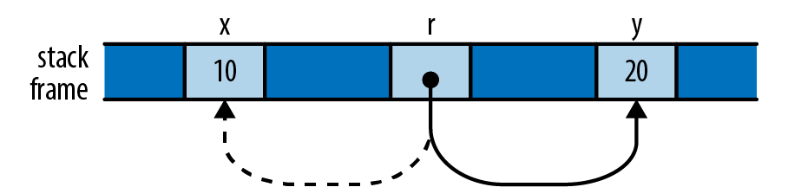
\includegraphics[width=0.8\textwidth]{../img/f5-1.png}
    \caption{引用r，现在指向y而不是x}
    \label{f5-1}
\end{figure}

代码的行为似乎太过于简单而不值一提：显然\texttt{r}现在会指向\texttt{y}，因为我们把\texttt{\&y}赋给了它。但我们指出这一点是因为C++的引用与此差别很大：如之前展示的一样，在C++中对一个引用赋值会把值存储在引用指向的对象。一旦一个C++引用被初始化之后，将没有任何方法让它指向别的东西。

\subsection{引用的引用}
Rust允许引用的引用：
\begin{minted}{Rust}
    struct Point { x: i32, y: i32 }
    let point = Point { x: 1000, y: 729 };
    let r: &Point = &point;
    let rr: &&Point &r;
    let rrr: &&&Point = &rr;
\end{minted}

（我们写出引用的类型是为了看得更清楚，但你可以省略它们，Rust可以推导出这里的所有类型。）\texttt{.}运算符寻找目标时需要解引用多次：
\begin{minted}{Rust}
    assert_eq!(rrr.y, 729);
\end{minted}

在内存中，这些引用按照\hyperref[f5-2]{图5-2}的形式排布。

\begin{figure}[htbp]
    \centering
    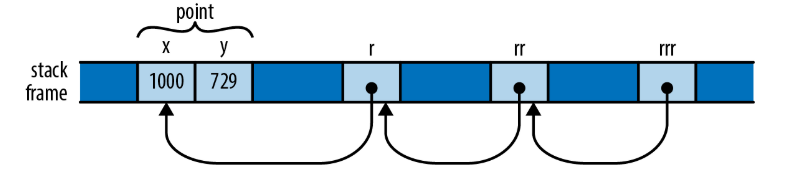
\includegraphics[width=0.8\textwidth]{../img/f5-2.png}
    \caption{引用的引用链}
    \label{f5-2}
\end{figure}

因此表达式\texttt{rrr.y}，在\texttt{rrr}的类型的引导下，实际上进行了3次解引用才得到了\texttt{Point}值，然后才能获得它的\texttt{y}字段。

\subsection{比较引用}

类似于\texttt{.}运算符，Rust比较运算符“看穿”任意数量的引用嵌套：
\begin{minted}{Rust}
    let x = 10;
    let y = 10;

    let rx = &x;
    let ry = &y;

    let rrx = &rx;
    let rry = &ry;

    assert!(rrx <= rry);
    assert!(rrx == rry);
\end{minted}

这里，最后的断言会成功，尽管\texttt{rrx}和\texttt{rry}指向不同的值（\texttt{rx}和\texttt{ry}），但因为\texttt{==}运算符会解除所有的引用然后对最终的值\texttt{x}和\texttt{y}进行比较。这几乎总是你想要行为，尤其是编写泛型函数时。如果你实际上是想知道两个引用是否指向相同的内存位置，你可以使用\texttt{std::ptr::eq}，它会按照地址比较引用：
\begin{minted}{Rust}
    assert!(rx == ry);              // 它们指向的对象相等
    assert!(!std::ptr:eq(rx, ry));  // 但是地址不同
\end{minted}

注意比较运算符的操作数的类型必须完全相同，包括引用：
\begin{minted}{Rust}
    assert!(rx == rrx);     // error：类型不匹配：`&i32` 和 `&&i32`
    assert!(rx == *rrx);    // Ok
\end{minted}

\subsection{引用永不为空}
Rust的引用永远不可能为空，没有类似C的\texttt{NULL}或C++的\texttt{nullptr}的值。引用没有默认初始值（不管什么类型，你不能在一个变量初始化之前使用它）并且Rust不允许把整数转换为引用（除了\texttt{unsafe}代码），因此你不能把0转换为引用。

C和C++经常使用空指针来表示没有值：例如，\texttt{malloc}函数会返回一个指向新内存块的指针，但如果没有足够的内存能够满足要求就会返回一个\texttt{nullptr}。在Rust里，如果你需要一个可能是引用可能是无的值，你可以使用类型\texttt{Option<\&T>}。在机器层面，Rust将\texttt{None}表示为空指针，将\texttt{Some(r)}（其中\texttt{r}是一个\texttt{\&T}类型的值）表示为非0的地址，因此\texttt{Option<\&T>}和C或C++中的可以为空的指针一样高效，然而它却是安全的：它的类型要求你在使用它之前要先检查它是不是\texttt{None}。

\subsection{借用任意表达式的引用}
C和C++只允许你对特定种类的表达式使用\texttt{\&}运算符，而Rust允许你借用任何表达式的引用：
\begin{minted}{Rust}
    fn factorial(n: usize) -> usize {
        (1..n+1).product()
    }
    let r = &factorial(6);
    // 算术运算符可以看穿一层引用
    assert_eq!(r + &1009, 1729);
\end{minted}

在类似这样的场景中，Rust简单的创建一个匿名变量来存储表达式的值，然后让引用指向它。匿名变量的生命周期依赖于你使用引用的方式：
\begin{itemize}
    \item 如果你立刻通过一个\texttt{let}语句把它赋值给了一个变量（或者将它变为了结构体或数组的一部分），那么Rust会让匿名变量的生命周期变得和\texttt{let}初始化的变量一样长。在上面的例子中，Rust将会对\texttt{r}引用的值进行这样的操作。
    \item 否则，匿名变量将只能生存到语句结束。在我们的示例中，存储\texttt{1009}的匿名变量只生存到\texttt{assert\_eq!}语句的结尾处。
\end{itemize}

如果你习惯于C或C++，这可能听起来很容易出错。但记住Rust永远不会让你写出产生悬垂引用的代码。如果引用被用在匿名变量的生命周期之外，Rust总是会在编译期向你报告这个问题。然后你可以把被引用的值保存在一个有恰当的生命周期的命名变量中来修复代码。

\subsection{切片和trait对象的引用}
我们至今展示的所有引用都只是简单的地址。然而，Rust还包括两种类型的\emph{胖指针}：包含值的地址和使用值所必需的额外信息的两个字的值。

切片的引用是一种胖指针，包括切片的起始地址和它的长度。我们在\hyperref[ch03]{第3章}中详细讨论了切片。

Rust的另一种胖指针类型是\emph{trait对象}，一个实现了特定trait的值的引用。一个trait对象包含值的地址和一个指向该值对trait的实现的指针，用于调用trait的方法。我们将在“\hyperref[traitobject]{trait对象}”一节中详细介绍trait对象。

除了携带了这些额外信息之外，切片和trait对象的引用和我们在这一章中目前见到的所有引用一样：它们并不获取所有权，不允许比引用对象生存得更久，可能是共享或者可变的，等等。

\section{引用安全}

正如我们目前为止展示的一样，引用与C和C++中的普通指针看起来非常像。但那些指针是不安全的，Rust怎么能保证引用的安全呢？可能最简单的发现规则的方法就是尝试去打破规则。

为了展示最基础的思想，我们将以最简单的例子开始，展示Rust是怎么保证引用在单个函数体里被正确使用。然后我们会看到在函数之间传递引用和在数据结构中对它们排序。这意味着要给函数和数据类型提供\emph{生命周期参数}，我们马上会解释它。最后，我们会展示一些Rust提供的用于简化常用模式的缩写。在这个过程中，我们会看到Rust是怎么指出错误代码并给出建议的解决方岸。

\subsection{借用一个局部变量}

这里有一个非常明显的例子。你不能借用一个局部变量的引用然后把它带出变量的作用域：
\begin{minted}{Rust}
    {
        let r;
        {
            let x = 1;
            r = &x;
        }
        assert_eq!(*r, 1);  // bad: reads memory `x` used to occupy
    }
\end{minted}

Rust的编译器会拒绝这个程序，并给出详细的错误消息：
\begin{minted}{text}
    error: `x` does not live long enough
      --> references_dangling.rs:8.5
       |
    7  |         r = &x;
       |             ^^ borrowed value does not live long enough
    8  |     }
       |     - `x` dropped here while still borrowed
    9  |     assert_eq!(*r, 1); // bad: reads memory `x` used to occupy
    10 | }
\end{minted}

Rust说\texttt{x}只生存到内层块的末尾，然而引用一直生存到外层块的末尾，因此它会变为悬垂指针，这是禁止的。

尽管对于人类来说很容易就能看出来这个程序是错误的，但Rust是如何得到这个结论的值得探究。每一个简单的例子都展示了Rust用于检查更多复杂代码的工具。

Rust尝试给你的程序中的每一个引用赋予一个\emph{生命周期}，这个生命周期要满足使用它的方式带来的约束。一个生命周期是一个引用可以安全使用的程序区间：可能是一条语句、一个表达式、也可能是一些变量的作用域，或者类似的区间。生命周期完全是Rust的编译期视图。在运行时引用只是一个地址，生命周期是它的类型的一部分，并没有运行时表示。

这个例子中，我们需要搞清楚三个生命周期的关系。变量\texttt{r}和\texttt{x}都有一个生命周期，从它们被初始化一直持续到编译器可以证明它们不会再被使用为止。第三个生命周期是一个引用类型的：我们从\texttt{x}借用并存储到\texttt{r}中的引用。

有一个规则应该非常明显：如果你有一个变量\texttt{x}，那么对\texttt{x}的引用不能比\texttt{x}的生命周期更长，如\hyperref[f5-3]{图5-3}所示。

\begin{figure}[htbp]
    \centering
    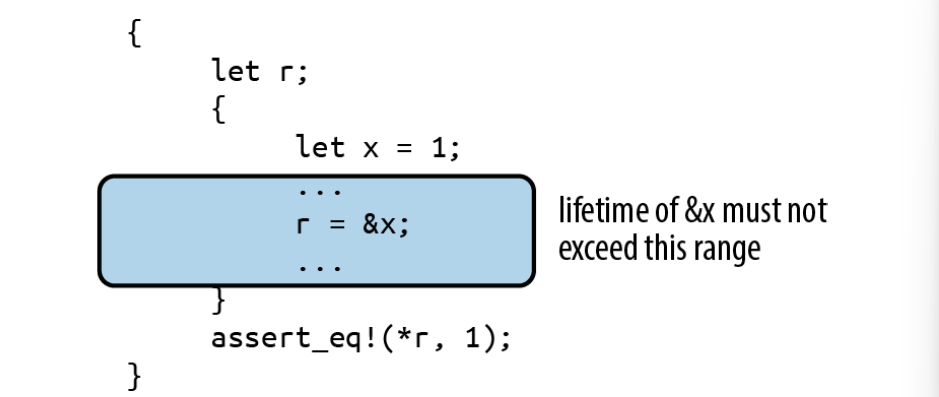
\includegraphics[width=0.9\textwidth]{../img/f5-3.png}
    \caption{\texttt{\&x}的合法生命周期}
    \label{f5-3}
\end{figure}

当\texttt{x}离开作用域之后，引用将变为悬垂指针。因此我们说变量的生命周期必须\emph{包含}或\emph{包括}它的引用的生命周期。

这里还有另一种约束：如果你把引用存储到变量\texttt{r}中，引用的生命周期必须覆盖变量的整个生命周期：从它初始化到最后一次使用它，如\hyperref[f5-4]{图5-4}所示。

\begin{figure}[htbp]
    \centering
    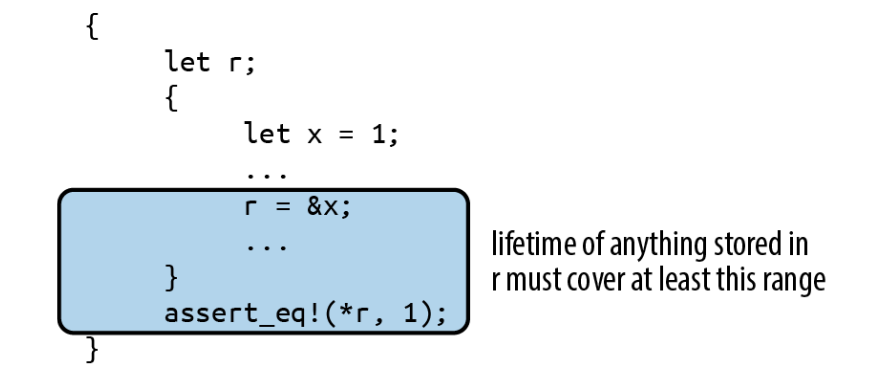
\includegraphics[width=0.9\textwidth]{../img/f5-4.png}
    \caption{存储在\texttt{r}中的引用的合法生命周期}
    \label{f5-4}
\end{figure}

如果引用不能和变量生存的一样长，那么在某些区域内指针\texttt{r}会变成悬垂指针。因此我们说引用的生命周期必须包含或包括存储它的变量的生命周期。

第一种约束限制了引用生命周期的上限，第二种约束限制了它的下限。Rust简单的尝试为每个引用找到一个满足这两个约束的生命周期。然而在我们的例子中，不存在这样的生命周期，如\hyperref[f5-5]{图5-5}所示。

\begin{figure}[htbp]
    \centering
    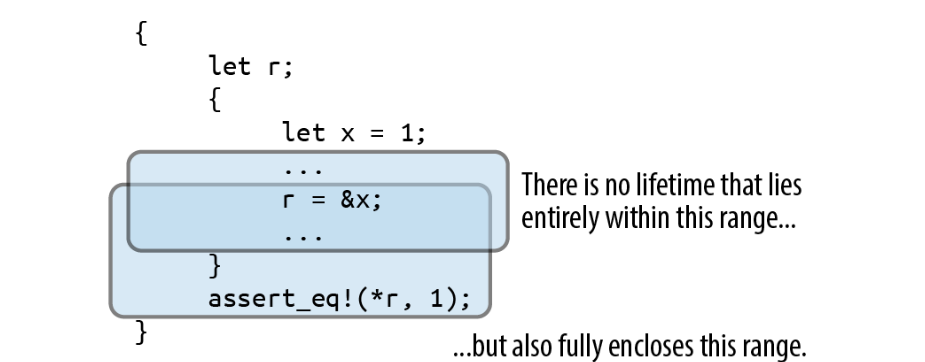
\includegraphics[width=0.9\textwidth]{../img/f5-5.png}
    \caption{一个引用的生命周期的限制互相矛盾}
    \label{f5-5}
\end{figure}

让我们考虑一个可以正常工作的不同的例子。我们有相同的约束：引用的生命周期必须被\texttt{x}的生命周期包含，但又要包含\texttt{r}的生命周期。但因为现在\texttt{r}的生命周期变小了，所以存在这样一个满足约束的生命周期，如\hyperref[f5-6]{图5-6}所示。

\begin{figure}[htbp]
    \centering
    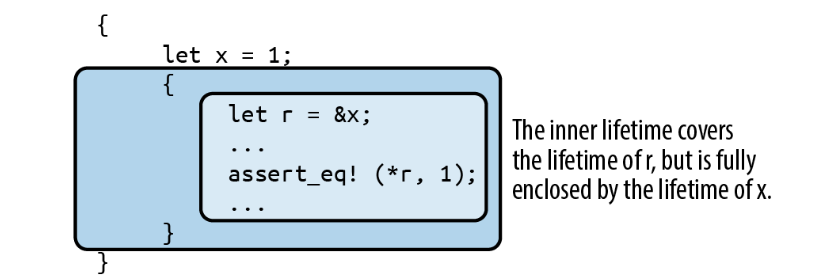
\includegraphics[width=0.9\textwidth]{../img/f5-6.png}
    \caption{一个引用的生命周期包括\texttt{r}的生命周期、但被\texttt{x}的生命周期包含}
    \label{f5-6}
\end{figure}

当你借用一个更大的数据结构中的一部分的引用时这些规则也自然地生效，例如引用vector的一个元素：
\begin{minted}{Rust}
    let v = vec![1, 2, 3];
    let r = &v[1];
\end{minted}

因为\texttt{v}拥有vector，vector又拥有它的元素，所以\texttt{v}的生命周期必须包含引用\texttt{\&v[1]}的生命周期。类似的，如果你把引用存储在了某些数据结构之中，那引用的生命周期必须包含这个数据结构的生命周期。例如，如果你创建了一个引用的vector，那么每个引用的生命周期都必须包含拥有这个vector的变量的生命周期。

这是Rust对所有代码进行的实质的处理。如果考虑更多的语言特性——例如复杂的数据结构和函数调用，只是会引入新的约束，但核心原则是不变的：首先，理解程序使用引用的方式所带来的约束；然后，找到满足这些约束的生命周期。这与C和C++程序员给自己施加的限制没有太大区别，区别在于Rust自己知道这些规则并且强迫它们执行。

\subsection{接受引用作为函数参数}

我当我们向函数传递引用时，Rust怎么保证函数安全地使用它？假设我们有一个函数\texttt{f}，这个函数接受一个引用，然后把它存储到一个全局变量中。我们之后会进行一些修改，不过这里有一个最初的版本：
\begin{minted}{Rust}
    // 这段代码有几个问题，不能通过编译。
    static mut STASH: &i32;
    fn f(p: &i32) { STASH = p; }
\end{minted}

Rust中的全局变量叫做\emph{静态变量}：它在程序开始时就被创建，直到程序终止时才被销毁。（类似其他的声明，Rust的模块系统控制静态变量在哪些部分可见，它们的“全局”只体现在生命周期上，而不是在可见性上）我们将在\hyperref[ch08]{第8章}中介绍静态变量，但现在我们只列出几条代码没有遵守的规则：
\begin{itemize}
    \item 每一个静态变量必须被初始化
    \item 可变的静态变量天然不是线程安全的（因为所有线程都可以在任何时间访问一个静态变量），即使在单线程程序中，它们也可能成为其它类型的重入问题的牺牲品。因为这些原因，你只能在\texttt{unsafe}块中使用可变的静态变量。在这个例子中我们并不关注那些特定的问题，我们只是把它放进\texttt{unsafe}块中，然后继续。
\end{itemize}

有了这些修改之后，我们有了下面的代码：
\begin{minted}{Rust}
    static mut STASH: &i32 = &128;
    fn f(p: &i32) { // 仍然不行
        unsafe {
            STASH = p;
        }
    }
\end{minted}

只差一步了，为了看到剩余的问题，我们需要写出一些Rust帮我们省略的东西。这里写的\texttt{f}的签名实际上是如下签名的缩写：
\begin{minted}{Rust}
    fn f<'a>(p: &'a i32) { ... }
\end{minted}

这里，生命周期\texttt{'a}（读作“tick A”）是\texttt{f}的一个\emph{生命周期参数}。你可以将\texttt{<'a>}读作“对于任何生命周期\texttt{'a}”，因此当我们写\texttt{fn f<'a>(p: \&'a i32)}时，我们定义了一个接受一个\texttt{i32}类型且带有任何给定生命周期\texttt{'a}的参数的函数。

尽管我们必须允许\texttt{'a}是任何生命周期，但如果它是最小的可能的生命周期的话会更好：例如恰好包含对\texttt{f}的调用。然后赋值语句就成了问题所在：
\begin{minted}{Rust}
    STASH = p;
\end{minted}

因为\texttt{STASH}在程序的整个执行过程中都存在，所以它持有的引用必须有相同长度的生命周期；Rust把这种生命周期称为\emph{\texttt{'static}生命周期}。但是\texttt{p}的生命周期是\texttt{'a}，意味着它可以是任意长度，只要包含对\texttt{f}的调用。因此，Rust拒绝了我们的代码：
\begin{minted}{text}
    error: explicit lifetime required in the type of `p`
      |
    5 | fn f(p: &i32) { // 仍然不行
      |         ____ help: add explicit lifetime `'static`
      |              to the type of `p`: `&'static i32`
    6 |     unsafe {
    7 |         STASH = p;
      |                 ^ lifetime `'static` required
\end{minted}

到这里，已经很明显了，我们的函数不能接受任意引用作为参数。但正如Rust指出的一样，它应该能接受一个有\texttt{'static}生命周期的引用：把这样一个引用存储到\texttt{STASH}不会导致悬垂指针。并且确实，下面的代码可以编译：
\begin{minted}{Rust}
    static mut STASH: &i32 = &10;

    fn f(p: &'static i32) {
        unsafe {
            STASH = p;
        }
    }
\end{minted}

这一次，\texttt{f}的签名指明了\texttt{p}必须是一个有\texttt{'static}生命周期的引用，因此将它存储在\texttt{STASH}中没有任何问题。我们只能将\texttt{f}用于其他静态变量的引用，但这是唯一一种保证\texttt{STASH}不会变为悬垂指针的方法。因此我们可以写：
\begin{minted}{Rust}
    static WORTH_POINTING_AT: i32 = 1000;
    f(&WORTH_POINTING_AT);
\end{minted}

因为\texttt{WORTH\_POINTING\_AT}是一个静态变量，所以\texttt{\&WORTH\_POINTING\_AT}的类型是\texttt{\&'static i32}，可以安全地传递给\texttt{f}。

稍微后退一步，注意一下我们这种修改的方式让\texttt{f}的签名发生了什么变化：原本的\texttt{f(p: \&i32)}变为了\texttt{f(p: \&'static i32)}。换句话说，如果不在函数签名中表明我们的意图，我们将不能写出一个把引用存储在全局变量中的函数。在Rust中，一个函数的签名总是暴露出函数体的行为。

反过来说，如果我们看到了一个函数签名例如\texttt{g(p: \&i32)}（或者写出了生命周期的\texttt{g<'a>(p: \&'a i32)}），我们将能辨别出它\emph{不会}把参数\texttt{p}存储在此次调用之外的变量中。我们不需要查看\texttt{g}的定义，\texttt{g}的签名已经告诉了我们它能做什么和不能做什么。当你想保持函数调用的安全性时，这一点会很有用。

\subsection{向函数传递引用}
现在我们已经展示了一个函数的签名怎么和它的函数体关联起来，让我们继续解释它怎么和函数的调用者联系起来。假设你有下面的代码：
\begin{minted}{Rust}
    // 这可以被更简洁地写为：fn g(p: &i32)
    // 但现在让我们写出生命周期
    fn g<'a>(p: &'a i32) { ... }

    let x = 10;
    g(&x);
\end{minted}

仅仅从\texttt{g}的签名，Rust知道它不会把\texttt{p}存储在生命周期超过此次调用的变量中：任何包含此次调用的生命周期\texttt{'a}都一定能正常工作。因此Rust为\texttt{\&x}选择了最小的可能的生命周期：也就是对\texttt{g}的调用。这满足了所有的约束：它的生命周期没有超过\texttt{x}、包含\texttt{g}的整个调用。因此这段代码可以通过检查。

注意尽管\texttt{g}有一个生命周期参数\texttt{'a}，我们在调用\texttt{g}时不需要提到它。你只需要在定义函数和类型时担心生命周期参数，当使用它们时，Rust会为你推断生命周期。

如果我们尝试把\texttt{\&x}传递给之前的接受静态引用参数的\texttt{f}函数，会发生什么呢？
\begin{minted}{Rust}
    fn f(p: &'static i32) { ... }

    let x = 10;
    f(&x);
\end{minted}

这样会编译失败：引用\texttt{\&x}不能生存的比\texttt{x}更久，但传递给\texttt{f}时，我们约束它至少要和\texttt{'static}生存的一样久。没有办法同时满足所有约束，所以Rust会拒绝这段代码。

\subsection{返回引用}
一种很常见的场景是一个函数接受一些数据结构的引用，然后返回一个指向这个结构中部分数据的引用。例如，这里有一个函数返回一个切片中最小的元素的引用：
\begin{minted}{Rust}
    // v应该至少有一个元素
    fn smallest(v: &[i32]) -> &i32 {
        let mut s = &v[0];
        for r in &v[1..] {
            if *r < *s { s = r; }
        }
        s
    }
\end{minted}

我们按照通常的方式省略了函数签名中的生命周期参数。当一个函数接收单个引用作为参数并返回单个引用时，Rust假设这两个引用一定有相同的生命周期。如果显式写出生命周期将是：
\begin{minted}{Rust}
    fn smallest<'a>(v: &'a [i32]) -> &'a i32 { ... }
\end{minted}

假设我们像这样调用\texttt{smallest}：
\begin{minted}{Rust}
    let s;
    {
        let parabola = [9, 4, 1, 0, 1, 4, 9];
        s = smallest(&parabola);
    }
    assert_eq!(*s, 0);  // 错误：s指向的元素已经被drop
\end{minted}

通过\texttt{smallest}的签名，我们能看出它的参数和返回值必须有相同的生命周期\texttt{'a}。在我们的调用中，参数\texttt{\&parabola}不能比\texttt{parabola}生存的久，然而\texttt{smallest}的返回值又至少要和\texttt{s}生存的一样久。不存在生命周期\texttt{'a}可以同时满足这两个约束，因此Rust拒绝了代码：
\begin{minted}{text}
    error: `parabola` does not live long enough
      --> references_lifetimes_propagated.rs:12:5
       |
    11 |         s = smallest(&parabola);
       |                       -------- borrow occurs here
    12 |     }
       |     ^ `parabola` dropped here while still borrowed
    13 |     assert_eq!(*s, 0); // bad: points to element of dropped array
       |                 - borrowed value needs to live until here
    14 | }
\end{minted}

移动对\texttt{s}的使用来保证它的生命周期被\texttt{parabola}的生命周期包含可以解决这个问题：
\begin{minted}{Rust}
    {
        let parabola = [9, 4, 1, 0, 1, 4, 9];
        let s = smallest(&parabola);
        assert_eq!(*s, 0);  // fine: parabola still alive
    }
\end{minted}

函数签名中的生命周期让Rust能获得传进函数的引用和函数返回的引用的关系，然后保证它们都被安全地使用。

\subsection{包含引用的结构体}























\chapter{表达式}\label{ch06}

\emph{LISP programmers know the value of everything, but the cost of nothing}

\begin{flushright}
    ——Alan Perlis, epigram \#55
\end{flushright}

在这一章中，我们将介绍Rust的\emph{表达式}，它是构成Rust函数体和大部分Rust代码的构建块。Rust中大部分都是表达式。在这一章中，我们将探索表达式的力量以及如何克服它的局限。我们还将介绍控制流，它在Rust中完全是以表达式为基础的，最后还要介绍Rust中的基本运算符如何单独和组合工作。

还有一些从技术角度应该划入这一类的概念，例如闭包和迭代器，因为足够重要因此我们之后会用单独的章节介绍它们。现在，我们希望能用尽可能少的页数介绍尽可能多的语法。

\section{表达式语言}

Rust表面上看上去像C家族的语言，但这其实是一个误解。在C语言中，\emph{表达式}和\emph{语句}之间有很大的不同。表达式是一些像这样的代码：
\begin{minted}{C}
    5 * (fahr-32) / 9
\end{minted}
而语句则是像这样的：
\begin{minted}{C}
    for (; begin != end; ++begin) {
        if (*begin == target)
            break;
    }
\end{minted}
表达式有值，但语句没有。

Rust是一种\emph{表达式语言}。这意味着它遵循了起源于Lisp的传统，也就是表达式负责完成所有工作。

在C中，\texttt{if}和\texttt{switch}是语句。它们并不产生值，也不能被用在表达式中间。在Rust中，\texttt{if}和\texttt{match}\emph{可以}产生值。我们已经在\hyperref[ch02]{第2章}中看到过一个产生数字值的\texttt{match}表达式：
\begin{minted}{Rust}
    pixels[r * bounds.0 + c] =
        match escapes(Complex { re: point.0, im: point.1 }, 255) {
            None => 0,
            Some(count) => 255 - count as u8
        };
\end{minted}

一个\texttt{if}表达式可以用于初始化一个变量：
\begin{minted}{Rust}
    let status =
        if cpu.temperature <= MAX_TEMP {
            HttpStatus::Ok
        } else {
            HttpStatus::ServerError  // server melted
        };
\end{minted}

一个\texttt{match}表达式可以被用作函数参数或宏的参数：
\begin{minted}{Rust}
    println!("Inside the vat, you see {}.",
        match vat.contents {
            Some(brain) => brain.desc(),
            None => "nothing of interest"
        });
\end{minted}

这解释了Rust为什么没有C的三元运算符\texttt{(expr1 ? expr2 : expr3))}。在C中，它是一种类似\texttt{if}语句的表达式。在Rust中这种写法是多余的，因为\texttt{if}表达式可以同时实现这两种功能。

C中的大部分控制流工具都是语句，在Rust中则全是表达式。

\section{优先级和结合性}

\hyperref[t6-1]{表6-1}总结了Rust的表达式语法。我们将在这一章中介绍所有这些表达式。运算符按照优先级从高到低的顺序列出。（类似于大多数编程语言，Rust使用\emph{运算符优先级}来决定当表达式中含有多个运算符时的运算顺序。例如，在表达式\texttt{limit < 2 * broom.size + 1}中，\texttt{.}运算符优先级最高，因此会先访问字段。）

\begin{longtable}{p{0.25\textwidth}p{0.35\textwidth}p{0.3\textwidth}}
    \caption{表达式}
    \label{t6-1} \\
    \hline
    \textbf{表达式类型} & \textbf{示例} & \textbf{相关trait} \\
    \hline
    数组字面量      & \texttt{[1, 2, 3]}         & \\
    重复数组字面量  & \texttt{[0; 50]}           & \\
    元组            & \texttt{(6, "crullers")}  & \\
    \cline{1-2}
    组合            & \texttt{(2 + 2)}             & \\
    块              & \texttt{\{ f(); g() \}}      & \\
    控制流表达式     & \texttt{if ok \{ f() \}}     & \\
                    & \texttt{if ok \{ 1 \} else \{ 0 \}}                   & \\
                    & \texttt{if let Some(x) = f() \{ x \} else \{ 0 \}}    & \\
                    & \texttt{match x \{ None => 0, \_ => 1 \}}             & \\
                    & \texttt{for v in e \{ f(v); \}}                       & \texttt{\hyperref[iter]{std::iter::IntoIterator}} \\
                    & \texttt{while ok \{ ok = f(); \}}                     & \\
                    & \texttt{while let Some(x) = it.next() \{ f(x); \}}    & \\
                    & \texttt{loop \{ next\_event(); \}}                    & \\
                    & \texttt{break}                  & \\
                    & \texttt{continue}               & \\
                    & \texttt{return 0}               & \\
    宏调用          & \texttt{println!("ok")}         & \\
    路径            & \texttt{std::f64::consts::PI}   & \\
    \cline{1-2}
    结构体字面量     & \texttt{Point \{x: 0, y: 0\}}     & \\
    \cline{1-2}
    元组字段访问    & \texttt{pair.0}   & \texttt{\hyperref[deref]{Deref}, \hyperref[deref]{DerefMut}} \\
    结构体字段访问  & \texttt{point.x}  & \texttt{\hyperref[deref]{Deref}, \hyperref[deref]{DerefMut}} \\
    方法调用       & \texttt{point.translate(50, 50)} & \texttt{\hyperref[deref]{Deref}, \hyperref[deref]{DerefMut}} \\
    函数调用       & \texttt{stdin()}   & \texttt{\hyperref[fn]{Fn(Arg0, ...) -> T}, \hyperref[fn]{FnMut(Arg0, ...) -> T}, \hyperref[fn]{FnOnce(Arg0, ...) -> T}} \\
    索引            & \texttt{arr[0]}   & \texttt{\hyperref[index]{Index}, \hyperref[index]{IndexMut}, \hyperref[deref]{Deref}, \hyperref[deref]{DerefMut}} \\
    \cline{1-2}
    错误检查        & \texttt{create\_dir("tmp")?}   & \\
    逻辑/位 NOT     & \texttt{!ok}  & \texttt{\hyperref[unop]{Not}} \\
    负             & \texttt{-num}  & \texttt{\hyperref[unop]{Neg}} \\
    解引用          & \texttt{*ptr} & \texttt{\hyperref[deref]{Deref}, \hyperref[deref]{DerefMut}} \\
    借用            & \texttt{\&val}    & \\
    \cline{1-2}
    类型转换    & \texttt{x as u32} \\
    \cline{1-2}
    乘法        & \texttt{n * 2}    & \texttt{\hyperref[biop]{Mul}} \\
    除法        & \texttt{n / 2}    & \texttt{\hyperref[biop]{Div}} \\
    余数（取模） & \texttt{n \% 2}   & \texttt{\hyperref[biop]{Rem}} \\
    \cline{1-2}
    加法        & \texttt{n + 1}    & \texttt{\hyperref[biop]{Add}} \\
    减法        & \texttt{n - 1}    & \texttt{\hyperref[biop]{Sub}} \\
    \cline{1-2}
    左移        & \texttt{n << 1}   & \texttt{\hyperref[biop]{Shl}} \\
    右移        & \texttt{n >> 1}   & \texttt{\hyperref[biop]{Shr}} \\
    \cline{1-2}
    位与        & \texttt{n \& 1}   & \texttt{\hyperref[biop]{BitAnd}} \\
    \cline{1-2}
    位异或      & \texttt{n \^ 1}   & \texttt{\hyperref[biop]{BitXor}} \\
    \cline{1-2}
    位或        & \texttt{n | 1}    & \texttt{\hyperref[biop]{BitOr}}  \\
    \cline{1-2}
    小于        & \texttt{n < 1}    & \texttt{\hyperref[cmp]{std::cmp::PartialOrd}} \\
    小于等于    & \texttt{n <= 1}   & \texttt{\hyperref[cmp]{std::cmp::PartialOrd}} \\
    大于        & \texttt{n > 1}    & \texttt{\hyperref[cmp]{std::cmp::PartialOrd}} \\
    大于等于    & \texttt{n >= 1}   & \texttt{\hyperref[cmp]{std::cmp::PartialOrd}} \\
    等于        & \texttt{n == 1}   & \texttt{\hyperref[equal]{std::cmp::PartialEq}} \\
    不等于      & \texttt{n != 1}   & \texttt{\hyperref[equal]{std::cmp::PartialEq}} \\   
    \cline{1-2}
    逻辑与      & \texttt{x.ok \&\& y.ok}       & \\
    \cline{1-2}
    逻辑或      & \texttt{x.ok || backup.ok}    & \\
    \cline{1-2}
    左闭右开区间 & \texttt{start .. stop}   & \\
    左闭右闭区间 & \texttt{start ..= stop}  & \\
    \cline{1-2}
    赋值        & \texttt{x = val}  & \\
    复合赋值    & \texttt{x *= 1}   & \texttt{\hyperref[assign]{MulAssign}} \\
                & \texttt{x /= 1}   & \texttt{\hyperref[assign]{DivAssign}} \\
                & \texttt{x \%= 1}  & \texttt{\hyperref[assign]{RemAssign}} \\
                & \texttt{x += 1}   & \texttt{\hyperref[assign]{AddAssign}} \\
                & \texttt{x -= 1}   & \texttt{\hyperref[assign]{SubAssign}} \\
                & \texttt{x <<= 1}  & \texttt{\hyperref[assign]{ShlAssign}} \\
                & \texttt{x >>= 1}  & \texttt{\hyperref[assign]{ShrAssign}} \\
                & \texttt{x \&= 1}  & \texttt{\hyperref[assign]{BitAndAssign}} \\
                & \texttt{x \^= 1}  & \texttt{\hyperref[assign]{BitXorAssign}} \\
                & \texttt{x |= 1}   & \texttt{\hyperref[assign]{BitOrAssign}} \\
    \cline{1-2}
    闭包        & \texttt{|x, y| x + y} & \\
\end{longtable}

所有可以链式使用的运算符都是左结合的。也就是说，一条运算链例如\texttt{a - b - c}被组合为\texttt{(a - b) - c}，而不是\texttt{a - (b - c)}。这些运算符可以被任意组合：
\begin{minted}{text}
    * / % + - << >> & ^ | && || as
\end{minted}
比较运算符、赋值运算符、范围运算符\texttt{.. }和\texttt{..=}不能被链式使用。

\section{块和分号}

\label{cast}

\chapter{错误处理}\label{ch07}
\chapter{crate与模块}\label{ch08}

\emph{This is one note in a Rust theme: systems programmers can have nice things.}

\begin{flushright}
    ——Robert O'Callahan, “\href{https://robert.ocallahan.org/2016/08/random-thoughts-on-rust-cratesio-and.html}{Random Thoughts on Rust: crates.io and IDEs}”
\end{flushright}

假设你在编写一个仿真蕨类植物从细胞开始生长的程序。你的程序就像蕨类一样，一开始非常简单，可能所有代码都在单个文件里——就像一个孢子。随着它逐渐成长，它开始逐渐建立起内部的结构，不同的片段负责不同的功能。它将分裂为多个文件，可能覆盖整个目录树。随着时间的推移，它可能会成为整个软件生态系统的重要组成部分 。对于任何成长到不仅仅是几个数据结构和几百行代码的程序，都必须要对代码进行组织。

这一章将会介绍Rust中用于组织程序的特性：crate和模块。我们还会介绍Rust crate的结构和分发相关的话题，包括如何编写文档和测试Rust代码，如何禁用不需要的编译器警告，如何使用Cargo来管理项目依赖和版本，如何在Rust的公开crate仓库：crates.io上发布开源的库，crate的版本如何演变，等等。我们将使用蕨类仿真程序作为我们的例子。

\section{Crate}

Rust程序由\emph{crates}组成。每一个crate都是一个完整的、一体的单元：一个库或可执行文件的所有代码、加上相关的测试、示例、工具、配置、以及一些其他东西。为了编写你自己的蕨类模拟器，你可能需要使用和3D图形、生物信息学、并行计算等相关的第三方库。这些库就像箱子一样（见\hyperref[f8-1]{图8-1}）。

\begin{figure}[htbp]
    \centering
    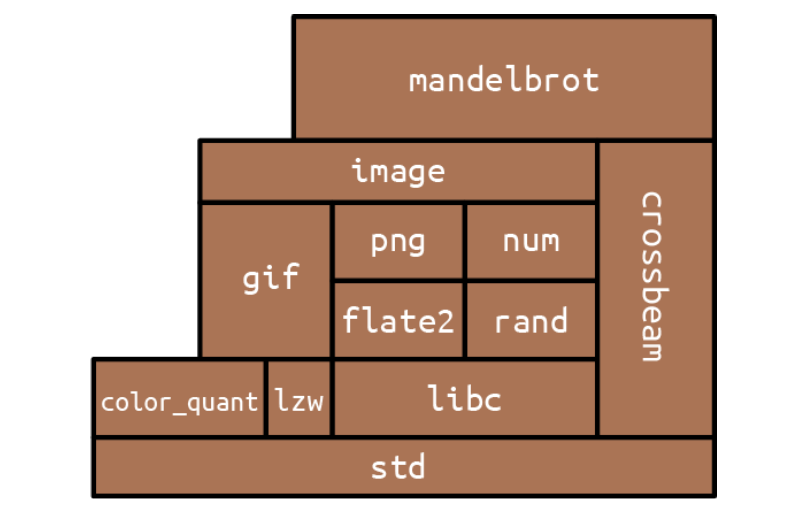
\includegraphics[width=0.9\textwidth]{../img/f8-1.png}
    \caption{一个crate和它的依赖}
    \label{f8-1}
\end{figure}

查看crate是什么以及它们是如何工作的最简单方法就是使用带有\texttt{--verbose}参数的\texttt{cargo build}来构建一个有一些依赖的程序。我们用\hyperref[mandelbrot]{一个并发的曼德勃罗集}作为示例。结果如下所示：
\begin{minted}{text}
    $ cd mandelbrot
    $ cargo clean   # delete previously compiled code
    $ cargo build --verbose
        Updating registry `https://github.com/rust-lang/crates.io-index`
     Downloading autocfg v1.0.0
     Downloading semver-parser v0.7.0
     Downloading gif v0.9.0
     Downloading png v0.7.0
    
    ... (downloading and compiling many more crates)

        Compiling jpeg-decoder v0.1.18
          Running `rustc
             --crate-name jpeg_decoder
             --crate-type lib
             ...
             --extern byteorder=.../libbyteorder-29efdd0b59c6f920.rmeta
             ...
        Compiling image v0.13.0
          Running `rustc
             --crate--name image
             --crate-type lib
             ...
             --extern byteorder=.../libbyteorder-29efdd0b59c6f920.rmeta
             --extern gif=.../libgif-a7006d35f1b58972.rmeta
             --extern jpeg_decoder=.../libjped_decoder-5c10558d0d57d300.rmeta
        Compiling mandelbrot v0.1.0 (/tmp/rustbook-test-files/mandelbrot)
          Running `rustc
             --edition=2018
             --crate-name mandelbrot
             --crate-type bin
             ...
             --extern crossbeam=.../libcrossbeam-f87b4b3d3284acc2.rlib
             --extern image=.../libimage-b5737c12bd641c43.rlib
             --extern num=.../libnum-1974e9a1dc582ba7.rlib -C link-arg=-fuse-ld=lld`
         Finished dev [unoptimized + debuginfo] target(s) in 16.94s
\end{minted}

我们重新格式化了\texttt{rustc}的命令行来改善可读性，并且删掉了很多和我们的讨论无关的编译器选项，用省略号(\ldots)代替了它们。

你可能还记得，当我们完成曼德勃罗集程序时，它的\emph{main.rs}包含几个引入其它crate的\\
\texttt{use}声明：
\begin{minted}{Rust}
    use num::Complex;
    // ...
    use image::ColorType;
    use image::png::PNGEncoder;
\end{minted}

我们还在\emph{Cargo.toml}中指定了每个crate的版本：
\begin{minted}{toml}
    [dependencies]
    num = "0.4"
    image = "0.13"
    crossbeam = "0.8"
\end{minted}

这里的\emph{依赖}指这个程序使用的其它crate，也就是我们依赖的代码。我们可以在\href{https://crates.io}{crates.io}中找到这些crate，那是Rust社区用于存放开源的crate的网站。例如，我们可以访问crates.io并搜索图片库来找到\texttt{image}库。crates.io上的每个crate的页面上会显示它的\emph{README.md}文件和到文档和源代码的链接，还有一行配置例如\texttt{image = "0.13"}，你可以复制这一行并添加到你的\emph{Crago.toml}中。这里显示的版本号直接用了我们在编写这个程序时这三个包的最新版本。

Cargo的输出说明了这些信息是如何被使用的。当我们运行\texttt{cargo build}时，Cargo会首先从crates.io下载这些crate的指定版本的源码。然后，它读取那些crate的\emph{Cargo.toml}文件，下载\emph{它们}的依赖，然后递归操作。例如，\texttt{image} crate的0.13.0版本的源代码中包含一个\emph{Cargo.toml}文件，内容如下：
\begin{minted}{toml}
    [dependencies]
    byteorder = "1.0.0"
    num-iter = "0.1.32"
    num-rational = "0.1.32"
    num-traits = "0.1.32"
    enum_primitive = "0.1.0"
\end{minted}

看到这些内容，Cargo知道在它可以使用\texttt{image}之前，它必须先拉取这些crate。我们称它们为\texttt{mandelbrot}的\emph{间接(transitive)}依赖。所有这些依赖的集合告诉了Cargo需要知道的有关如何构建和构建顺序的一切信息，它被称为crate的\emph{依赖图}。Cargo自动处理依赖图和间接依赖的能力是程序员们付出时间和努力的一大胜利。

当获得了源代码之后，Cargo会编译所有的crate。它会运行Rust的编译器\texttt{rustc}，一次编译依赖图中的一个crate。当编译这些库时，Cargo会使用\texttt{--crate-type lib}选项。这告诉\texttt{rustc}不要寻找\texttt{main()}函数，而是产生一个包含编译过代码的\emph{.rlib}文件，这个文件可以被用于创建可执行文件和其他\emph{.rlib}文件。

当编译程序时，Cargo会使用\texttt{--crate-type bin}，编译的结果将是一个目标平台的二进制可执行文件：例如在Windows上就是\emph{mandelbrot.exe}。

对于每一个\texttt{rustc}命令，Cargo都会传递\texttt{--extern}选项，给出crate用到的每一个库的名称。这样，当\texttt{rustc}看到一行类似于\texttt{use image::png::PNGEncoder}的代码时，它可以分辨出\texttt{image}是另一个crate的名字，而且Cargo传递的选项让它知道该从哪里寻找编译好的crate。Rust的编译器需要访问这些\emph{.rlib}文件，因为它们包含编译好的库中的代码。Rust将会将代码静态链接到最终的可执行文件中。\emph{.rlib}还包含类型信息，因此Rust可以通过检查确保我们在代码中使用的库的特性确实存在而且被正确使用。它还包含一份crate的public内联函数、泛型、宏、特性的拷贝，这些东西只有当Rust看到我们如何使用它们时才可以将它们编译为机器代码。

\texttt{cargo build}支持各种选项，其中的大部分都超出了本书的范围，不过我们在这里会提到其中一个：\texttt{cargo build --release}会生成优化后的构建。Release构建运行得更快，但需要更长的时间来编译，而且它们不检查整数溢出、跳过\texttt{debug\_assert!()}断言，并且它们在panic时生成的堆栈追踪通常不太可靠。

\subsection{版本}

Rust有极强的兼容性保证。任何在Rust 1.0中能编译的代码必须在Rust 1.50或者1.900（如果发布了的话）中也能编译。


但有时社区会遇到一些令人信服的扩展语言的建议，这可能会导致旧代码不能再编译。例如，经过了多次讨论之后，Rust确定了一种支持异步编程的语法，将标识符\texttt{async}和\texttt{await}重新用作关键字（见\hyperref[ch20]{第20章}）。但这项语言的改变可能会导致使用\texttt{async}或者\texttt{await}作为变量名的代码不能再编译。

为了在不破坏这些现有代码的前提下演变，Rust使用了\emph{版本}。Rust的2015版本和Rust 1.0兼容。2018版本将\texttt{async}和\texttt{await}改为关键字、精简了模块系统、还引入了一些和2015版本不兼容的其它语言更改。每个crate在\emph{Cargo.toml}文件中的\texttt{package}节中用一行类似如下的说明指定Rust的版本：
\begin{minted}{Rust}
    edition = "2018"
\end{minted}

如果缺少这个关键字，将会假设使用2015版本，因此旧的crate完全不需要做任何更改。但如果你想使用异步函数或者新的模块系统，你需要确保\emph{Cargo.toml}中有\texttt{edition = "2018"}（或者可能更新的版本）。

Rust保证编译器将总是接受语言的所有版本，并且程序可以自由混合使用不同版本编写的crate。即使一个2015版本的crate依赖一个2018版本的crate也没有问题。换句话说，一个crate的版本只影响它的代码是如何被构建的，版本的区别只体现在代码编译的时候。这意味着没有必要更新旧的版本来适配现代Rust的生态。类似的，也没有必要将crate保持在旧版本来避免影响到它的用户。你只需要在想使用新的语言特性时更改自己代码中的版本。

版本并不是每年都会更新，只有当Rust项目觉得有必要出新版本的时候才会更新。例如，没有2020版本。把\texttt{edition}设置为\texttt{"2020"}将会导致错误。\href{https://doc.rust-lang.org/stable/edition-guide}{Rust版本指南}介绍了每一个版本中的变化，并提供了版本系统的背景知识。

使用最新版本几乎总是一个好主意，尤其是新编写代码时。\texttt{cargo new}会默认创建最新版本的项目。本书中将始终使用2018版本。

如果你有一个用更旧版本的Rust编写的crate，\texttt{cargo fix}命令也许可以帮你自动把代码更新到更新的版本。Rust版本指南详细解释了\texttt{cargo fix}命令。

\subsection{构建配置}
有几个\emph{Cargo.toml}中的配置选项可以影响到\texttt{cargo}生成的\texttt{rustc}命令行（\hyperref[t8-1]{表8-1}）。

\begin{table}[htbp]
    \centering
    \caption{Cargo.toml配置节}
    \label{t8-1}
    \begin{tabular}{ll}
        \hline
        \textbf{命令行}     & \textbf{使用到的Cargo.toml节}   \\
        \hline
        \texttt{cargo build} & \texttt{[profile.dev]}   \\
        \rowcolor{tablecolor}
        \texttt{cargo build --release} & \texttt{[profile.release]} \\
        \texttt{cargo test}  & \texttt{[profile.test]}  \\
    \end{tabular}
\end{table}

通常默认的行为就足够了，但我们会发现一个例外是你想使用一个profiler——一个用于测量程序使用CPU时间情况的工具。为了从profiler获取最准确的数据，你将同时需要优化（通常只在release构建中可用）和调试符号（通常只在debug构建中可用）。为了同时启用两者，在\emph{Cargo.toml}中添加：
\begin{minted}{toml}
    [profile.release]
    debug = true    # 允许在release构建中启用调试符号
\end{minted}

\texttt{debug}设置控制是否给\texttt{rustc}传递\texttt{-g}选项。有了这个配置，当你输入\\
\texttt{cargo build --release}时，你将会得到一个带有调试符号的二进制文件。优化的设置将不会被影响。

\href{https://doc.rust-lang.org/cargo/reference/manifest.html}{Cargo文档}中列出了很多其他你可以在\emph{Cargo.toml}中调整的设置。

\section{模块}

如果说crate决定了项目之间的代码共享，那么\emph{模块}则决定了项目\emph{内部}的代码组织。它们扮演了Rust中的命名空间——一种包含函数、类型、常量等内容的容器，这些模块组成了你的Rust程序或库。一个模块看起来类似于这样：

\begin{minted}{Rust}
    mod spores {
        use cells::{Cell, Gene};

        /// 成熟蕨类植物产生的细胞。它会随着风飘散，
        /// 这也是蕨类生命周期的一部分。一个孢子会成长为一个原叶体——
        /// 一个宽达5mm的完整的独立有机体。它会产生受精卵，
        /// 这些受精卵会成长为新的蕨类植物（植物的性别很复杂）。
        pub struct Spore {
            ...
        }

        /// 模拟通过减数分裂产生孢子的过程。
        pub fn produce_spore(factory: &mut Sporangium) -> Spore {
            ...
        }

        // 提取一个孢子中的基因。
        pub(crate) fn genes(spore: &Spore) -> Vec<Gene> {
            ...
        }

        /// 混合基因为减数分裂做准备（分裂间期的一部分）。
        fn recombine(parent: &mut Cell) {
            ...
        }

        ...
    }
\end{minted}

模块是\emph{item}的集合，\texttt{item}是命名的特性，例如本例中的\texttt{Spore}结构体和两个函数。\texttt{pub}关键字将item设为公有的，因此可以从模块外部访问。

把函数标记为\texttt{pub(crate)}，意味着它在这个crate中任何地方都可以访问，但不作为外部接口的一部分公开。它不能被其他crate使用，也不会在crate的文档中显示。

任何没有被标记为\texttt{pub}的都是私有的，只能在定义它的模块和子模块中使用：
\begin{minted}{Rust}
    let s = spores::produce_spore(&mut factory);    // ok
    
    spores::recombine(&mut cell);   // 错误：`recombine`是私有的
\end{minted}

将item标记为\emph{pub}通常称为“导出”这个item。

这一节的剩余部分将覆盖使用模块所需要了解的细节：
\begin{itemize}
    \item 我们会展示如果需要的话怎么嵌套模块和把它们分布在不同的文件和目录中。
    \item 我们会解释Rust从其他模块中引用item的路径语法，并展示怎么导入item，这样就不需要每次都写出完整的路径。
    \item 我们会接触Rust对结构体字段的细粒度控制。
    \item 我们会介绍\emph{prelude}模块，它通过收集几乎所有用户都会用到的常见导入来减少重复的导入。
    \item 我们会展示\emph{常量}和\emph{静态量}，这是两种为了清晰和一致性而设计的定义命名变量的方式。
\end{itemize}

\subsection{嵌套模块}

模块可以嵌套，事实上一个模块只是一些子模块的集合的情况是很常见的：
\begin{minted}{Rust}
    mod plant_structures {
        pub mod roots {
            ...
        }
        pub mod stems {
            ...
        }
        pub mod leaves {
            ...
        }
    }
\end{minted}

如果你想要让嵌套模块中的一个item对其他crate可见，那需要保证将它\emph{和所有嵌套包含它的模块}标记为public。否则你会看到一个类似这样的警告：
\begin{minted}{text}
    warning: function is never used: `is_square`
      --> src/crates_unused_items.rs:23:9
       |
    23 | /         pub fn is_square(root: &Root) -> bool {
    24 | |             root.cross_section_shape().is_square()
    25 | |         }
       | |_________^
       |
\end{minted}

可能这个函数这时确实是死代码。但如果你是想将它用在其他crate中，Rust会让你明白它实际上并不可见。你需要保证嵌套包含它的模块也都被标记为\texttt{pub}。

也可以声明\texttt{pub(super)}，让一个item只在父模块中可见。\texttt{pub(in <path>)}可以让它在一个指定的父模块和其后代中可见。这在深层嵌套的模块中很有用：
\begin{minted}{Rust}
    mod plant_structures {
        pub mod roots {
            pub mod products {
                pub(in crate::plant_structures::roots) struct Cytokinin {
                    ...
                }
            }

            use products::Cytokinin;    // ok: 在`roots`模块中
        }

        use roots::products::Cytokinin; // error: `Cytokinin`是私有的
    }

    // error: `Cytokinin`是私有的
    use plant_structures::roots::products::Cytokinin;
\end{minted}

通过这种方式，我们可以写出一个有数量庞大的代码和完整的模块层次结构的程序，不管这些模块的关系如何，我们都可以将整个程序写在单个文件里。

但实际上以这种方式来工作非常的痛苦，因此还有另一种方案。

\subsection{单独文件中的模块}\label{ModInFile}
一个模块还可以这么写：
\begin{minted}{Rust}
    mod spores;
\end{minted}

之前，我们还在花括号中包含了\texttt{spores}模块的主体。这里，我们通过这种方式告诉Rust编译器\texttt{spores}模块在一个单独的叫\emph{spores.rs}的文件里：
\begin{minted}{Rust}
    // spores.rs

    /// 成熟蕨类植物产生的一个细胞...
    pub struct Spore {
        ...
    }

    /// 模拟减数分裂产生孢子的过程。
    pub fn produce_spore(factory: &mut Sporangium) -> Spore {
        ...
    }

    /// 从一个孢子中提取基因。
    pub(crate) fn genes(spore: &Spore) -> Vec<Gene> {
        ...
    }

    /// 混合基因为减数分裂做准备（分裂间期的一部分）。
    fn recombine(parent: &mut Cell) {
        ...
    }
\end{minted}

\emph{spores.rs}只包含组成模块的item。它并不需要任何说明来表明它是一个模块。

这个\texttt{spores}模块和我们在上一节中展示的版本的\emph{唯一}不同就是代码的位置。有关公有性和私有性的规则和之前完全相同。Rust从来不会单独编译模块，即使它们在单独的文件里。当你构建一个Rust的crate的时候，你总是要重新编译它里面所有的模块。

一个模块也可以有自己的目录。当Rust看到\texttt{mod spores;}时，它会检查\emph{spores.rs}和\\
\emph{spores/mod.rs}，如果这两个文件都不存在或者都存在就会报错。本例中因为\texttt{spores}模块没有任何子模块，所以我们使用了\emph{spores.rs}。但考虑一下我们之前写的\texttt{plant\_structures}模块。如果我们决定将那个模块和它的三个子模块分割在单独的文件中，最终的项目看起来就是这样：
\begin{minted}{text}
    fern_sim/
    |-- Cargo.toml
    |-- src/
        |-- main.rs
        |-- spores.rs
        |-- plant_structures/
            |-- mod.rs
            |-- leaves.rs
            |-- roots.rs
            |-- stems.rs
\end{minted}

在\emph{main.rs}中，我们声明了\texttt{plant\_structures}模块：
\begin{minted}{Rust}
    pub mod plant_structures;
\end{minted}

这会导致Rust去加载\emph{plant\_structures/mod.rs}，这个文件里又声明了三个子模块：
\begin{minted}{Rust}
    // 在plant_structures/mod.rs中
    pub mod roots;
    pub mod stems;
    pub mod leaves;
\end{minted}

这三个模块的内容都被存储在单独的文件中，分别命名为\emph{leaves.rs}、\emph{roots.rs}、\emph{stems.rs}，和\emph{mod.rs}一样在\texttt{plant\_structures}目录下。

使用同名的文件和目录来组成模块也是可行的。例如，如果\texttt{stems}需要包含两个分别叫\texttt{xylem}和\texttt{phloem}的模块，我们可以选择将\texttt{stems}保留在\emph{plant\_structures/stems.rs}中，然后添加一个新的\texttt{stems}目录：
\begin{minted}{text}
    fern_sim/
    |-- Cargo.toml
    |-- src/
        |-- main.rs
        |-- spores.rs
        |-- plant_structures/
            |-- mod.rs
            |-- leaves.rs
            |-- roots.rs
            |-- stems/
            |   |-- phloem.rs
            |   |-- xylem.rs
            |
            |-- stems.rs
\end{minted}

然后在\emph{stems.rs}中声明这两个新的子模块：
\begin{minted}{Rust}
    // 在plant_structures/stems.rs中
    pub mod xylem;
    pub mod phloem;
\end{minted}

这三种方式——模块在自己单独的文件中、模块在自己同名的目录中的\emph{mod.rs}中，模块在自己单独的文件中并有一个同名的目录包含子模块——给了模块系统足够的灵活性来支撑你需要的任何程序结构。

\subsection{路径和导入}
\texttt{::}运算符用于访问模块中的特性。你的项目中任何地方的代码都可以通过路径来引用任何标准库的特性：
\begin{minted}{Rust}
    if s1 > s2 {
        std::mem::swap(&mut s1, &mut s2);
    }
\end{minted}

\texttt{std}是标准库的名称。路径\texttt{std}指向标准库的顶层模块。\texttt{std::mem}是在标准库中的一个子模块，\texttt{std::mem::swap}是\texttt{std::mem}模块中的一个public函数。

你可以始终用这种方式编写所有的代码，每当你需要圆或字典时都写出\\
\texttt{std::f64::consts::PI}和\texttt{std::collections::HashMap::new}，但这样太过繁琐，而且难以阅读。替代方案是把一些特性\emph{导入}用到它们的模块：
\begin{minted}{Rust}
    use std::mem;

    if s1 > s2 {
        mem::swap(&mut s1, &mut s2);
    }
\end{minted}

\texttt{use}声明会导致\texttt{mem}变为\texttt{std::mem}在整个块或模块中的一个局部别名。

你也可以写\texttt{std::mem::swap}来导入\texttt{swap}函数本身，而不是\texttt{mem}模块。然而，我们之前的方式被认为是最佳的风格：引入类型、trait和模块（例如\texttt{std::mem}）然后使用相对路径访问函数、常量和其他成员。

可以一次导入若干个名字：
\begin{minted}{Rust}
    use std::collections::{HashMap, HashSet};   // 导入两个
    
    use std::fs::{self, File};  // 导入`std::fs`和`std::fs::File`
    
    use std::io::prelude::*;    // 导入所有内容
\end{minted}

也可以写出所有的单独导入：
\begin{minted}{Rust}
    use std::collections::HashMap;
    use std::collections::HashSet;

    use std::fs;
    use std::fs::File;

    // std::io::prelude中的所有public item：
    use std::io::prelude::Read;
    use std::io::prelude::Write;
    use std::io::prelude::BufRead;
    use std::io::prelude::Seek;
\end{minted}

你可以使用\texttt{as}导入一个item并同时给它一个不同的局部名称：
\begin{minted}{Rust}
    use std::io::Result as IOResult;

    // 返回类型等价于`std::io::Result<()>`
    fn save_spore(spore: &Spore) -> IOResult<()>
    ...
\end{minted}

模块并不会\emph{自动}从父模块中继承名称。例如，假设我们的\emph{proteins/mod.rs}有如下内容：
\begin{minted}{Rust}
    // proteins/mod.rs
    pub enum AminoAcid { ... }
    pub mod synthesis;
\end{minted}

那么\emph{synthesis.rs}里的代码并不会自动导入类型\texttt{AminoAcid}：
\begin{minted}{Rust}
    // proteins/synthesis.rs
    pub fn synthesis(seq: &[AminoAcid]) // 错误：找不到类型`AminoAcid`
        ...
\end{minted}

每一个模块都会以空白的状态开始，必须导入它使用的名称：
\begin{minted}{Rust}
    // proteins/synthesis.rs
    use super::AminoAcid;   // 显式地从父模块中导入
    pub fn synthesize(seq: &[AminoAcid]) // ok
        ...
\end{minted}

默认情况下，路径是相对于当前模块的：
\begin{minted}{Rust}
    // 在proteins/mod.rs中

    // 从子模块中导入
    use synthesis::synthesize;
\end{minted}

\texttt{self}也是当前模块的同义词，因此我们可以写：
\begin{minted}{Rust}
    // 在proteins/mod.rs中

    // 导入一个枚举中的名字
    // 这样我们可以用`Lys`来表示赖氨酸，而不是`AminoAcid::Lys`
    use self::AminoAcid::*;
\end{minted}

或者简写为：
\begin{minted}{Rust}
    // 在proteins/mod.rs中

    use AminoAcid::*;
\end{minted}

（这里的\texttt{AminoAcid}的例子，有些违背我们之前提到的只导入类型、trait和模块的风格。如果我们的程序包含很长的氨基酸序列，那么根据奥威尔的第六原则：“Break any of these rules sooner than say anything outright barbarous.”（绝不要用粗俗语言，为此可以打破上面任一规则。）这么做也是有道理的。

路径中的\texttt{super}和\texttt{crate}关键字有特殊的含义：\texttt{super}指代父模块，\texttt{crate}指代包含当前模块的crate。

使用相对于crate根的路径而不是相对于当前模块的路径可以使在项目中移动代码变得更容易，因为这样的话就算当前模块的路径变了，导入也不会出错。例如，我们可以使用\texttt{crate}来写\emph{synthesis.rs}：
\begin{minted}{Rust}
    // proteins/synthesis.rs
    use crate::proteins::AminoAcid; // 显式的相对于crate根的导入

    pub fn synthesize(seq: &[AminoAcid]) // ok
        ...
\end{minted}

子模块可以通过\texttt{use super::*}访问父模块中的私有item。

如果你有一个模块和当前正在使用的某一个模块同名，那么引用它们的时候就要小心了。例如，如果你的程序在\emph{Cargo.toml}列出了\texttt{image} crate依赖，同时还有一个模块叫\texttt{image}，那么以\texttt{image}开头的路径将会导致歧义：
\begin{minted}{Rust}
    mod image {
        pub struct Sampler {
            ...
        }
    }

    // 错误：这是指向`image`模块，还是`image` crate？
    use image::Pixels;
\end{minted}

即使\texttt{image}模块没有\texttt{Pixels}类型，这个歧义也会被认为是错误：如果之后又添加了\texttt{Pixels}的定义，那么可能会改变路径指向的内容，这可能会令人迷惑。

为了解决歧义，Rust有一种特殊的路径称为\emph{绝对路径}，它们以\texttt{::}开头，将总是指向一个外部的crate。为了指向\texttt{image} crate中的\texttt{Pixels}类型，你可以写：
\begin{minted}{Rust}
    use ::image::Pixels;    // `image` crate的`Pixels`
\end{minted}

为了指向你自己的模块中的`Sampler`类型，你可以写：
\begin{minted}{Rust}
    use self::image::Sampler;   // `image`模块的`Sampler`
\end{minted}

模块和文件的概念并不相同，但模块和Unix文件系统中的文件和目录存在自然的类比关系。\texttt{use}关键字创建别名，就像\texttt{ln}命令创建链接。路径类似于文件名，有绝对路径和相对路径两种形式。\texttt{self}和\texttt{super}类似于\texttt{.}和\texttt{..}这两个特殊的目录。

\subsection{标准prelude}
我们之前说每个模块都以“空白的状态”开始，但事实上并不是\emph{完全}空白的状态。

其中一点是，标准库\texttt{std}被自动链接到每个项目。这意味着你总是可以使用\texttt{std::whatever}\\
这种方式来引用\texttt{std}里的item，例如\texttt{std::mem::swap()}。另外，一些特殊的常见名称，例如\texttt{Vec}和\texttt{Result}也被包含在\emph{标准prelude}中并且被自动导入。具体的行为就好像是包括根模块在内的每个模块都以如下导入开始：
\begin{minted}{Rust}
    use std::prelude::v1::*;
\end{minted}

标注的prelude包含一些通用的trait和类型。

在\hyperref[ch02]{第2章}中时，我们提到了库有时会提供叫\texttt{prelude}的模块。但\texttt{std::prelude::v1}是唯一一个自动导入的。将一个模块命名为\texttt{prelude}只是一个惯例，告诉用户他应该导入\texttt{*}。

\subsection{pub use声明}
即使\texttt{use}声明只是别名，它们也可以是公有的：
\begin{minted}{Rust}
    // in plant_structures/mod.rs
    ...
    pub use self::leaves::Leaf;
    pub use self::roots::Root;
\end{minted}

这意味着\texttt{Leaf}和\texttt{Root}是\texttt{plant\_structures}模块里的public item。它们实际上只是\\
\texttt{plant\_structures::leaves::Leaf}和\texttt{plant\_structures::roots::Root}的别名。

标准的prelude就是以一系列\texttt{pub}导入的方式实现的。

\subsection{pub结构体字段}
模块可以包含用户用\texttt{struct}关键字定义的自定义结构体类型。我们将在\hyperref[ch09]{第9章}中介绍细节，但这是一个了解模块如何和结构体字段的可见性交互的好时机。

一个简单的结构体类似这样：
\begin{minted}{Rust}
    pub struct Fern {
        pub roots: RootSet,
        pub stems: StemSet
    }
\end{minted}

一个结构体的所有字段，包括私有字段，都可以在定义结构体的整个模块及其子模块中访问，在模块之外，只有公有的字段才可以被访问。

事实证明通过模块来实现访问控制，而不是像Java和C++那样通过类来实现，对于程序设计将是很大的帮助。不仅能减少重复“getter”和“setter”方法，还能消除类似C++中\texttt{friend}声明的需求。一个模块中可以定义几个紧密结合的类型，例如\texttt{frond::LeafMap}和\\
\texttt{frond::LeafMapIter}，让它们能按需互相访问彼此的私有字段，同时对程序中的其他部分隐藏实现的细节。

\subsection{静态量和常量}\label{static}

除了函数、类型和嵌套模块之外，模块里还可以定义\emph{常量}和\emph{静态量}。

\texttt{const}关键字定义常量，语法类似于\texttt{let}，除了它必须被标记为\texttt{pub}以及要显式写出类型。还有，为了方便，常量一般都用\texttt{UPPERCASE\_NAMES}：
\begin{minted}{Rust}
    pub const ROOM_TEMPERATURE: f64 = 20.0;     // 摄氏度
\end{minted}

\texttt{static}关键字定义静态量，和\texttt{const}的用法几乎一样：
\begin{minted}{Rust}
    pub static ROOM_TEMPERATURE: f64 = 68.0;    // 华氏温度
\end{minted}

常量有些类似于C++中的\texttt{\#define}，值被编译进代码中每一个使用它的地方。一个静态量就是一个在程序开始之前就初始化并持续到程序退出的变量。在代码中使用常量表示幻数和字符串。使用静态量表示更大规模的数据，或者用于需要借用全局常量的引用时。

没有\texttt{mut}常量。静态量可以被标记为\texttt{mut}，但就像我们在\hyperref[ch05]{第5章}中讨论的一样，Rust没有任何方法强制实现\texttt{mut}静态量的独占访问。因此，这种变量天生线程不安全，safe代码完全不能使用它们：
\begin{minted}{Rust}
    static mut PACKETS_SERVED: usize = 0;

    println!("{} served", PACKETS_SERVED);  // 错误：使用了可变的静态量
\end{minted}

Rust不鼓励全局可变的状态。关于替代方案的讨论，见\nameref{globalvar}一节。

\section{将程序变为库}

当你的蕨类模拟器完成之后，你发现你需要不止一个程序。假设你还有一个命令行程序运行这个模拟器并把结果保存到文件中。现在，你想要编写其他程序来对保存的结果进行科学分析、实时渲染成长中的植物、渲染逼真的植物等等。所有这些程序都要共享基本的蕨类模拟器的代码。你需要创建一个库。

第一步是将你现有的项目分解为两部分：一个库crate和一个可执行文件。前者包含所有的共享代码，后者包含只有命令行程序才需要的代码。

为了展示怎么做到这一点，让我们给出一个简单粗暴的示例程序：
\begin{minted}{Rust}
    struct Fern {
        size: f64,
        growth_rate: f64
    }

    impl Fern {
        /// 模拟一个蕨类植物一天地成长
        fn grow(&mut self) {
            self.size *= 1.0 + self.growth_rate;
        }
    }

    /// 运行蕨类模拟器模拟几天的变化
    fn run_simulation(fern: &mut Fern, days: usize) {
        for _ in 0 .. days {
            fern.grow();
        }
    }

    fn main() {
        let mut fern = Fern {
            size: 1.0,
            growth_rate: 0.001
        };
        run_simulation(&mut fern, 1000);
        println!("final fern size: {}", fern.size);
    }
\end{minted}

我们假设这个程序有一个普通的\emph{Cargo.toml}文件：
\begin{minted}{toml}
    [package]
    name = "fern_sim"
    version = "0.1.0"
    authors = ["You <you@example.com>"]
    edition = "2018"
\end{minted}

将这个程序变为库是很简单的。只需要如下步骤：
\begin{enumerate}
    \item 将文件\emph{src/main.rs}重命名为\emph{src/lib.rs}
    \item 给\emph{src/lib.rs}里将作为库的公开特性的item添加\texttt{pub}关键字
    \item 暂时把\texttt{main}函数移动到一个别的临时文件中。我们将很快回来处理它。
\end{enumerate}

最后的\emph{src/lib.rs}文件看起来像这样：
\begin{minted}{Rust}
    pub struct Fern {
        pub size: f64,
        pub growth_rate: f64
    }

    impl Fern {
        /// 模拟一个蕨类植物一天地成长
        pub fn grow(&mut self) {
            self.size *= 1.0 + self.growth_rate;
        }
    }

    /// 运行蕨类模拟器模拟几天的变化
    pub fn run_simulation(fern: &mut Fern, days: usize) {
        for _ in 0 .. days {
            fern.grow();
        }
    }
\end{minted}

注意我们不需要更改\emph{Cargo.toml}中的任何内容。因为我们的最精简的\emph{Cargo.toml}会保持Cargo的默认行为。默认情况下，\texttt{cargo build}会查看源代码目录下的文件然后判断要构建什么。当它看到\emph{src/lib.rs}文件，它就知道要构建一个库。

\emph{src/lib.rs}里的代码组成了库的\emph{根模块}。其他使用我们库的crate可以访问根模块里的公有item。

\section{src/bin目录}\label{src/bin}

想让原本的\texttt{fern\_sim}程序再次工作也非常简单：Cargo有一些内建的支持，可以让较小的程序和库存在同一个crate中。

事实上，Cargo自身就是用这种方式编写的。它的大部分代码都在一个Rust库里。我们在本书中至今为止用过的\texttt{cargo}命令行程序只是一个简单的包装程序，它会调用库来完成真正的工作。库和命令行程序\href{https://github.com/rust-lang/cargo}{在同一个源代码仓库中}。

我们也可以把程序和库放在同一个crate中。将以下代码放入\emph{src/bin/efern.rs}的文件中：
\begin{minted}{Rust}
    use fern_sim::{Fern, run_simulation};

    fn main() {
        let mut fern = Fern {
            size: 1.0,
            growth_rate: 0.001
        };
        run_simulation(&mut fern, 1000);
        println!("final fern size: {}", fern.size);
    }
\end{minted}

这个\texttt{main}函数就是我们之前放在一边的那个。我们添加了\texttt{use}声明来使用\texttt{fern\_sim} crate里的一些item：\texttt{Fern}和\texttt{run\_simulation}。也就是说，我们像使用库一样使用了那个crate。

因为我们把这个文件放在了\emph{src/bin}里，所以下次运行\texttt{cargo build}时，Cargo将会同时编译\texttt{fren\_sim}库和这个程序。我们可以使用\texttt{cargo run --bin efern}来运行\texttt{efern}程序。可以通过使用\texttt{--verbose}参数来查看Cargo运行的命令，大概是这样：
\begin{minted}{text}
    $ cargo build --verbose
       Compiling fern_sim v0.1.0 (file:///.../fern_sim)
         Running `rustc src/lib.rs --crate-name fern_sim --crate-type lib ...`
         Running `rustc src/bin/efern.rs --crate-name efern --crate-type bin ...`
    $ cargo run --bin efern --verbose
           Fresh fern_sim v0.1.0 (file:///.../fern_sim)
         Running `target/debug/efern`
    final fern size: 2.7169239322355985
\end{minted}

我们仍然不需要修改\emph{Cargo.toml}中的任何内容，Cargo的默认行为是查看源文件然后进行判断。它会自动把\emph{src/bin}里的\emph{.rs}文件当作额外的程序来构建。

我们也可以在\emph{src/bin}目录下通过子目录来构建更大的程序。假设我们想要提供另一个程序在屏幕上绘制蕨类植物，但绘制代码比较多而且是模块化的，因此它应该有自己的文件。我们可以将第二个程序放在单独的子目录中：
\begin{minted}{text}
    fern_sim/
    |-- Cargo.toml
    |-- src/
        |-- bin/
            |-- efern.rs
            |-- draw_fern/
                |-- main.rs
                |-- draw.rs
\end{minted}

把更大的可执行程序存放在自己的目录中的优势是不会打乱库代码和\texttt{src/bin}目录。

当然，既然现在\texttt{fern\_sim}是一个库，那么我们还有另一种选择。我们可以把这个程序放入单独的项目中，在一个完全独立的目录中，在它的\emph{Cargo.toml}中列出\texttt{fern\_sim}作为依赖：
\begin{minted}{toml}
    [dependencies]
    fern_sim = { path = "../fern_sim" }
\end{minted}

可能这正是你之后编写其他蕨类模拟程序时采用的方法。\emph{src/bin}目录只适合像\texttt{efern}和\\
\texttt{draw\_fern}这样的简单程序。

\section{属性}\label{attribute}

Rust程序中的任何item都可以用\emph{属性}修饰。属性是Rust中向编译器传递指令和建议的语法。例如，假设你得到了如下警告：
\begin{minted}{text}
    libgit2.rs: warning: type `git_revspec` should have a camel case name
        such as `GitRevspec`, #[warn(non_camel_case_types)] on by default
\end{minted}

但是你选择这个名字是有原因的，你并不希望Rust发出警告。你可以通过给类型加上\texttt{\#[allow]}属性来禁用警告：
\begin{minted}{Rust}
    #[allow(non_camel_case_types)]
    pub struct git_revspec {
        ...
    }
\end{minted}

条件编译是另一个通过属性来实现的特性，这个属性叫\texttt{\#[cfg]}：
\begin{minted}{Rust}
    // 只有当我们在构建Android应用时才在项目中包含这个模块
    #[cfg(target_os = "android")]
    mod mobile;
\end{minted}

\texttt{\#[cfg]}的完整语法见\href{https://doc.rust-lang.org/reference/conditional-compilation.html}{Rust参考手册}，\hyperref[t8-2]{表8-2}中列出了最常用的选项。

\begin{table}[htbp]
    \centering
    \caption{最常用的\texttt{\#[cfg]}选项}
    \label{t8-2}
    \begin{tabular}{p{0.2\textwidth}p{0.7\textwidth}}
        \hline
        \textbf{\texttt{\#[cfg]}选项}   & \textbf{编译的条件} \\
        \hline
        \texttt{test}   & 测试模式时（用\texttt{cargo test}或者\texttt{rustc --test}编译时） \\
        \rowcolor{tablecolor}
        \texttt{debug\_assertions} & 调试断言开始时（通常在非优化构建中） \\
        \texttt{unix}   & 为Unix系统编译时，包括macOS \\
        \rowcolor{tablecolor}
        \texttt{windows}& 为Windows编译时 \\
        \texttt{target\_pointer\_width = "64"} & 目标平台是64位时。其他可能的值是\texttt{"32"} \\
        \rowcolor{tablecolor}
        \texttt{target\_arch = "x86\_64"} & x86-64架构特定。其他值：\texttt{"x86", "arm", "aarch64", "powerpc", "powerpc64", "mips"} \\
        \texttt{target\_os = "macos"} & macOS特定。其他值：\texttt{"windows", "ios", "android", "linux", "freebsd", "openbsd", "netbsd", "dragonfly"} \\
        \rowcolor{tablecolor}
        \texttt{feature = "robots"} & 启用用户自定义特性\texttt{"robots"}时（用\texttt{cargo build --feature robots}或者\texttt{rustc --cfg feature='"robots"'}）。特性在\href{https://doc.rust-lang.org/cargo/reference/manifest.html}{\emph{Cargo.toml}的\texttt{[features]}节中声明}。 \\
        \texttt{not}(\emph(A)) & \emph{A}不满足时。为了让一个函数有两种不同的实现，可以将其中一个标记为\texttt{\#[cfg(X)]}，另一个表记为\texttt{\#[cfg(not(X))]}。 \\
        \rowcolor{tablecolor}
        \texttt{all}(\emph{A}, \emph{B}) & 当\emph{A}和\emph{B}都满足时（等价于\texttt{\&\&}）。 \\
        \texttt{any}(\emph{A}, \emph{B}) & 当\emph{A}或\emph{B}满足时（等价于\texttt{||}）。 \\
    \end{tabular}
\end{table}

有时，我们需要关心函数的内联展开，这是一种我们通常乐意让编译器实现的一种优化。我们可以使用\texttt{\#[inline]}属性来实现内联：
\begin{minted}{Rust}
    /// 调整相互渗透下，两个相邻细胞中的各种离子的浓度
    #[inline]
    fn do_osmosis(c1: &mut Cell, c2: &mut Cell) {
        ...
    }
\end{minted}

在一种特殊情况下，如果没有\texttt{\#[inline]}一定\emph{不会}发生内联。就是当一个crate中的一个函数或方法在另一个crate中被调用时，除非它是泛型的（有泛型参数）或者被显式标记为\texttt{\#[inline]}，否则它一定不会被内联展开。

另外，编译器只是把\texttt{\#[inline]}当作一个建议。Rust也支持\texttt{\#[inline(always)]}来要求一个函数必须在每一次被调用时内联展开；和\texttt{\#[inline(never)]}来要求一个函数永远不会被内联展开。

有一些属性，例如\texttt{\#[cfg]}和\texttt{\#[allow]}，可以被用于整个模块，然后作用于模块里的所有东西。而另一些，例如\texttt{\#[test]}和\texttt{\#[inline]}只能用于单独的item。正如你可能期待的一样，每个属性都是定制的，并且有自己的一组受支持的参数。Rust的参考手册详细列出了\href{https://doc.rust-lang.org/reference/attributes.html}{所有支持的属性}。

为了将一个属性用于整个crate，可以在\emph{main.rs}或者\emph{lib.rs}文件的最前边添加属性，并用\texttt{\#!}来代替\texttt{\#}，像这样：
\begin{minted}{Rust}
    // libgit2_sys/lib.rs
    #![allow(non_camel_case_types)]

    pub struct git_revspec {
        ...
    }

    pub struct git_error {
        ...
    }
\end{minted}

\texttt{\#!}告诉Rust将一个属性附加到作用域里的每一个item，而不是下一个item：在这个例子中，\texttt{\#![allow]}属性作用于整个\texttt{libgit2\_sys} crate，而不仅仅是\texttt{struct git\_revspec}。

\texttt{\#!}还可以在函数体内、结构体定义内等地方使用，但它通常被用在一个文件的开头，来将一个属性附加到整个模块或crate。一些属性总是使用\texttt{\#!}语法，因为它们只能被用于整个crate。

例如，\texttt{\#![feature]}属性可以打开Rust语言和库里的\emph{unstable}特性。这些特性都是实验性的，因此可能会有bug或者可能会在将来修改或者删除。例如，正如下面那段代码一样，Rust对追踪宏展开例如\texttt{assert!}有实验性的支持，但是因为这个支持是实验性的，因此你必须安装nightly版本的Rust并且显式声明你要使用宏追踪的特性：
\begin{minted}{Rust}
    #![feature(trace_macros)]
    
    fn main() {
        // 我想知道assert_eq!实际上到底被替换成了什么代码
        trace_macros!(true);
        assert_eq!(10*10*10 + 9*9*9, 12*12*12 + 1*1*1);
        trace_macros!(false);
    }
\end{minted}

随着时间的推移，Rust队伍有时会\emph{标准化}一个实验特性，这样它就会成为语言标准的一部分。然后\texttt{\#![feature]}特性就会变得多余，Rust会生成一个警告建议你删除它。

\section{测试和文档}

正如我们在\nameref{test}一节中看到的一样，Rust中内建了一个简单的单元测试框架。测试是用\texttt{\#[test]}属性标记的普通函数：
\begin{minted}{Rust}
    #[test]
    fn math_works() {
        let x: i32 = 1;
        assert!(x.is_positive());
        assert_eq!(x + 1, 2);
    }
\end{minted}

\texttt{cargo test}会运行项目中的所有测试：
\begin{minted}{text}
    $ cargo test
       Compiling math_test v0.1.0 (file:///.../math_test)
         Running target/release/math_test-e31ed91ae51ebf22
    
    running 1 test
    test math_works ... ok

    test result: ok. 1 passed; 0 failed; 0 ignored; 0 measuerd; 0 filtered out
\end{minted}
（你也可能会看到一些有关“doc-tests”的输出，我们将在稍后讨论它。）

测试的行为和你的crate是可执行程序还是库没有关系。你可以通过向Cargo传递参数来运行指定的测试：\texttt{cargo test math}会运行名称中包含\texttt{math}的所有测试。

测试通常使用Rust标准库里的\texttt{assert!}和\texttt{assert\_eq!}宏。若\texttt{expr}为真，\texttt{assert!(expr)}断言会成功；否则它会panic，并导致测试失败。\texttt{assert\_eq!(v1, v2)}类似于\texttt{assert!(v1 == v2)}，除了当断言失败时，它会同时打印出两个操作数的值。

也可以在普通的代码中使用这两个宏，但注意即使是release构建\texttt{assert!}和\texttt{assert\_eq!}也会被包含进去。使用\texttt{debug\_assert!}和\texttt{debug\_assert\_dq!}来编写只在debug构建时才会检查的断言。

为了测试错误的情况，需要向测试添加\texttt{\#[should\_panic]}属性：
\begin{minted}{Rust}
    /// 正如我们在上一章中说的一样，
    /// 只有当除0会导致panic时这个测试才能通过
    #[test]
    #[allow(unconditional_panic, unused_must_use)]
    #[should_panic(expected="divide by zero")]
    fn test_divide_by_zero_error() {
        1 / 0;  // 应该panic！
    }
\end{minted}

在这个例子中，我们需要添加\texttt{allow}属性来告诉编译器允许我们写一些可以静态证明一定会panic的代码，然后进行除法并丢弃结果值。因为通常情况下，编译器会阻止这种愚蠢的代码。

你也可以在测试中返回\texttt{Result<(), E>}。只要错误类型实现了\texttt{Debug} trait（这是通常的情况），你就可以使用\texttt{?}略过\texttt{Ok}的情况返回一个\texttt{Result}：
\begin{minted}{Rust}
    use std::num::ParseIntError;

    /// 只有当"1204"是个有效的数字时这个测试才能通过
    #[test]
    fn main() -> Result<(), ParseIntError> {
        i32::from_str_radix("1024", 10)?;
        Ok(())
    }
\end{minted}

用\texttt{\#[test]}标记的函数会条件编译。普通的\texttt{cargo build}或者\texttt{cargo build --release}会跳过测试代码。但当你运行\texttt{cargo test}时，Cargo会编译程序两次：一次是用普通方式编译，另一次是在启用测试和测试工具的情况下编译。这意味着如果需要的话，你的单元测试可以和要测试的代码放在一起，这样可以访问内部的实现细节，并且没有运行时开销。然而，这可能会导致一些警告。例如：
\begin{minted}{Rust}
    fn roughly_equal(a: f64, b: f64) -> bool {
        (a - b).abs() < 1e-6
    }

    #[test]
    fn trig_works() {
        use std::f64::const::PI;
        assert!(roughly_equal(PI.sin(), 0.0));
    }
\end{minted}

在省略测试代码的构建中，\texttt{roughly\_equal}可能未被使用，Rust会警告：
\begin{minted}{text}
    $ cargo build
       Compiling math_test v0.1.0 (file:///.../math_test)
    warning: function is never used: `roughly_equal`
     --> src/crates_unused_testing_function.rs:7:1
      |
    7 | / fn roughly_equal(a: f64, b: f64) -> bool {
    8 | |     (a - b).abs() < 1e-6    
    9 | | }
      | |_^
      |
       = note: #[warn(dead_code)] on by default
\end{minted}

因此，当你的测试足够复杂需要支持的代码的时候，将它们放在一个\texttt{tests}模块中并使用\texttt{\#[cfg]}属性将整个模块声明为测试模式特定：
\begin{minted}{Rust}
    #[cfg(test)]    // 只有在测试时才包含这个模块
    mod tests {
        fn roughly_equal(a: f64, b: f64) -> bool {
            (a - b).abs() < 1e-6
        }

        #[test]
        fn trig_works() {
            use std::f64::const::PI;
            assert!(roughly_equal(PI.sin(), 0.0));
        }
    }
\end{minted}

Rust的测试工具默认会使用多线程同时运行多个测试，这是你的Rust代码线程安全的一个附带的好处。为了禁用并行测试，运行\texttt{cargo test -- --test-threads 1}。（第一个\texttt{--}确保\texttt{cargo test}会把\texttt{--test-threads}选项传递给测试的可执行程序）如果想运行单个测试，运行\texttt{cargo test testname}。这意味着从技术上讲，我们在\hyperref[ch02]{第2章}中展示的曼德勃罗程序并不是那一章中的第二个多线程程序，而是第三个！\nameref{test}一节中运行的\texttt{cargo test}才是第一个。

通常来说，测试工具只会显示失败的测试的输出。为了显示通过的测试的输出，可以运行\texttt{cargo test -- --no-capture}。

\subsection{集成测试}
你的蕨类模拟器的规模仍然在增长。你决定将所有主要的代码放进一个库里，这样可以被很多可执行程序使用。模拟最终使用\emph{fern\_sim.rlib}库的用户使用它的方式对它进行一些测试将是一个好主意。另外，你还有一些首先从二进制文件中加载保存的模拟器的测试，将这些很大的测试文件保存在\texttt{src}目录中是很尴尬的。集成测试可以帮忙解决这两个问题。

集成测试是\texttt{src}目录下的\emph{tests}目录中的\emph{.rs}文件。当你运行\texttt{cargo test}时，Cargo会将每一个集成测试编译成独立的crate，然后和你的库以及Rust的测试工具链接。这里有一个例子：
\begin{minted}{Rust}
    // tests/unfurl.rs - Fiddleheads unfurl in sunlight

    use fern_sim::Terrarium;
    use std::time::Duration;

    #[test]
    fn test_fiddlehead_unfurling() {
        let mut world = Terrarium::load("tests/unfurl_files/fiddlehead.tm");
        assert!(world.fern(0).is_furled());
        let one_hour = Duration::from_secs(60 * 60);
        world.apply_sunlight(one_hour);
        assert!(world.fern(0).is_fully_unfurled());
    }
\end{minted}

集成测试之所以有价值，部分原因是它们从crate外部看待你的crate，就像一个用户一样。它们测试crate的public API。

\texttt{cargo test}会同时运行单元测试和集成测试。为了只运行特定文件中的集成测试——例如\emph{tests/unfurl.rs}——使用命令\texttt{cargo test --test unfurl}。

\subsection{文档}
命令\texttt{cargo doc}为你的库生成HTML文档：
\begin{minted}{text}
    $ cargo doc --no-deps --open
     Documenting fern_sim v0.1.0 (file:///.../fern_sim)
\end{minted}

\texttt{--no-deps}选项告诉Cargo只为\texttt{fern\_sim}自身生成文档，不要为它依赖的crate生成文档。

\texttt{--open}选项告诉Cargo稍后在你的浏览器中打开文档。

结果如\hyperref[f8-2]{图8-2}所示。Cargo会把新的文档文件保存在\emph{target/doc}中，起始页面是\\
\emph{target/doc/fern\_sim/index.html}。

\begin{figure}[htbp]
    \centering
    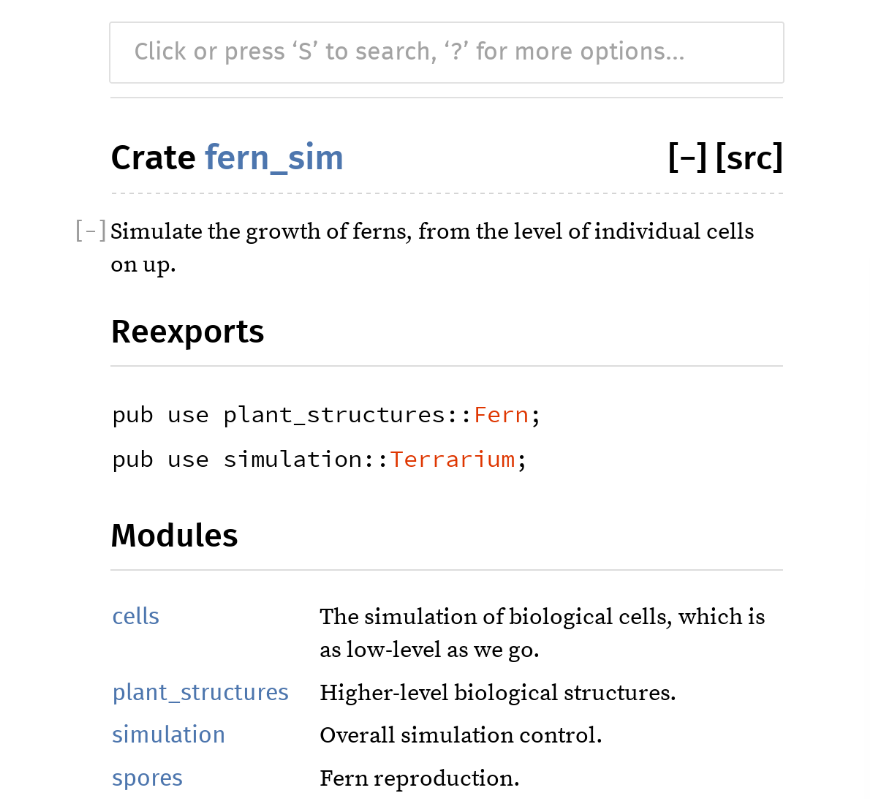
\includegraphics[width=0.9\textwidth]{../img/f8-2.png}
    \caption{\texttt{rustdoc}生成的文档示例}
    \label{f8-2}
\end{figure}

文档从你的库中的\texttt{pub}特性生成，加上你为它们编写的任何\emph{文档注释}。我们在这一章中已经看到过一些文档注释了。它们看起来像普通的注释：
\begin{minted}{Rust}
    /// 模拟减数分裂产生孢子的过程。
    pub fn produce_spore(factory: &mut Sporangium) -> Spore {
        ...
    }
\end{minted}
但当Rust看到它们是以三个斜杠开头时，它会把它们当作\texttt{\#[doc]}属性。Rust将上面的示例看作和下面的代码等价：
\begin{minted}{Rust}
    #[doc = "模拟减数分裂产生孢子的过程。"]
    pub fn produce_spore(factory: &mut Sporangium) -> Spore {
        ...
    }
\end{minted}

当你编译一个库或可执行程序时，这些属性并不会改变任何东西，但当你生成文档时，public特性的文档注释将会被包含在输出中。

同样的，以\texttt{//!}开头的注释被当作\texttt{\#![doc]}属性，这个属性会被附加到作用域中，通常是一个模块或者crate。例如，你的\emph{fern\_sim/src/lib.rs}文件看起来可能像这样：
\begin{minted}{Rust}
    //! 从独立的细胞开始，
    //! 模拟蕨类植物的生长。
\end{minted}

文档注释的内容被当做Markdown，一种简单HTML格式的速记符号。星号可以用作\texttt{*\emph{italics}*}和\texttt{**\textbf{bold type}**}，空行被当作段落结束，等等。你也可以包含HTML标签，它们会被逐字符拷贝到格式化文档。

Rust中的文档注释的一个特殊特性是Markdown链接可以使用Rust的item路径而不是相对URL来指明它们引用的item，例如\texttt{leaves::Leaf}。Cargo将会查找路径指向的内容，并创建指向正确文档页面中正确位置的链接。例如，这段代码生成的文档会链接到\texttt{VascularPath}、\texttt{Leaf}和\texttt{Root}的页面：
\begin{minted}{Rust}
    /// 创建并返回一个 [`VascularPath`] ，
    /// 它代表营养从给定的 [`Root`][r] 传输到给定的 [`Leaf`](leaves::Leaf) 的路径。
    ///
    /// [r]: roots::Root
    pub fn trace_path(leaf: &leaves::Leaf, root: &roots::Root) -> VascularPath {
        ...
    }
\end{minted}

你还可以添加搜索别名来使用内建的搜索特性让item更容易被找到。在crate的文档中搜索“path”或者“route”将会导向\texttt{VascularPath}：
\begin{minted}{Rust}
    #[doc(alias = "route")]
    pub struct VascularPath {
        ...
    }
\end{minted}

你可以使用\texttt{`backticks`}在文本中间创建代码片段。输出时，这些片段将会用等宽字体显示。更大的代码示例可以通过缩进四个空格来显示：
\begin{minted}{Rust}
    /// 文档注释中的一个代码块
    ///
    ///    if samples::everything().works() {
    ///        println!("ok");
    ///    }
\end{minted}
你也可以使用Markdown-fenced代码块，效果和上面一样：
\begin{minted}{Rust}
    /// 另一个片段，但是写法不同：
    /// 
    /// ```
    /// if samples::everything().works() {
    ///     println!("ok");
    /// }
    /// ```
\end{minted}

不管你用哪种方式，当你在文档注释中包含代码块的时候会发生一件有趣的事：Rust会自动把它当做一个测试。

\subsection{文档测试}
当你运行Rust库crate中的测试时，Rust会通过检查确保文档中出现的所有代码都能运行并正常工作。它将文档注释中出现的所有代码作为单独的可执行程序crate编译，然后和库链接并运行。

这里有一个文档测试的例子。运行\texttt{cargo new --lib ranges}（\texttt{--lib}参数告诉Cargo我们要创建一个库crate，而不是可执行程序crate）并将下列代码加到\emph{ranges/src/lib.rs}中：
\begin{minted}{Rust}
    use std::ops::Range;

    /// 如果两个范围重叠就返回true
    ///
    ///     assert_eq!(ranges::overlap(0..7, 3..10), true);
    ///     assert_eq!(ranges::overlap(1..5, 101..105), false);
    ///
    /// 如果有一个范围是空的，视为不重叠。
    ///
    ///     assert_eq!(ranges::overlap(0..0, 0..10), false);
    ///
    pub fn overlap(r1: Range<usize>, r2:Range<usize>) -> bool {
        r1.start < r1.end && r2.start < r2.end &&
            r1.start < r2.end && r2.start < r1.end
    }
\end{minted}

文档注释中的这两个小代码块将会出现在\texttt{cargo doc}生成的文档中，如\hyperref[f8-3]{图8-3}所示。

\begin{figure}[htbp]
    \centering
    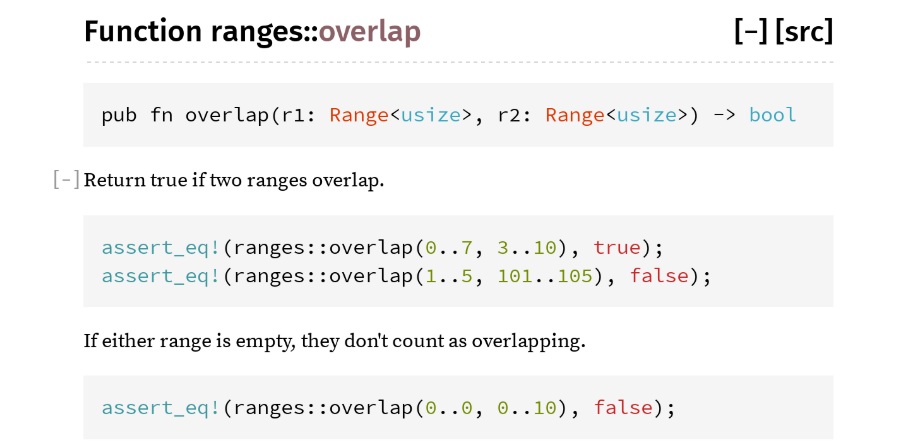
\includegraphics[width=0.8\textwidth]{../img/f8-3.png}
    \caption{文档注释会展示一些文档测试}
    \label{f8-3}
\end{figure}

它们也会成为两个单独的测试：
\begin{minted}{text}
    $ cargo test
       Compiling ranges v0.1.0 (file:///.../ranges)
    ...
       Doc-tests ranges

    running 2 tests
    test overlap_0 ... ok
    test overlap_1 ... ok

    test result: ok. 2 passed; 0 failed; 0 ignored; 0 measuerd; 0 filtered out
\end{minted}

如果你向Cargo传递\texttt{--verbose}参数，你将会看到它用\texttt{rustdoc --test}来运行这两个测试。\texttt{rustdoc}会把每个示例代码存储在单独的文件中，加上少量的样本代码来生成两个程序。这是第一个：
\begin{minted}{Rust}
    use ranges;
    fn main() {
        assert_eq!(ranges::overlap(0..7, 3..10), true);
        assert_eq!(ranges::overlap(1..5, 101..105), false);
    }
\end{minted}

这是第二个：
\begin{minted}{Rust}
    use ranges;
    fn main() {
        assert_eq!(ranges::overlap(0..0, 0..10), false);
    }
\end{minted}
如果程序能成功编译和运行，那么就可以通过测试。

这两段示例代码都包含了断言，但那只是因为在这种情况下，断言适用于编写文档。文档测试背后的目的不是让你把所有测试都放在注释里，而是让你写出最可能的用法的示例，然后Rust确保你文档中的代码示例确实可以编译并运行。

通常一个最小化的能工作的示例还包含一些细节，例如导入或初始化代码。这些是让代码能编译所必需的，但并不重要，不应该在文档中显示。为了隐藏代码示例中的某一行，可以在行的开始加上\texttt{\#}和一个空格：
\begin{minted}{Rust}
    /// 开启光照，并运行模拟器一段时间
    ///
    ///     # use fern_sim::Terrarium;
    ///     # use std::time::Duration;
    ///     # let mut tm = Terrarium::new();
    ///     tm.apply_sunlight(Duration::from_secs(60));
    ///
    pub fn apply_sunlight(&mut self, time: Duration) {
        ...
    }
\end{minted}

有时在文档中展示一个包含\texttt{main}函数的完整的示例程序会很有帮助。如果那些细节代码已经出现在了你的代码示例中，那你显然不会再希望\texttt{cargo}自动添加它们，因为这样会导致无法编译。因此\texttt{rustdoc}将所有包含字符串\texttt{fn main}的代码块视为完整的程序，不会再添加任何东西。

可以为特定的代码块禁用测试。为了告诉Rust编译你的示例，但并不真的运行它，可以使用带有\texttt{no\_run}注解的fenced代码块：
\begin{minted}{Rust}
    /// 将所有的本地培养皿上传到在线的gallery。
    ///
    /// ```no_run
    /// let mut session = fern_sim::connect();
    /// session.upload_all();
    /// ```
    pub fn upload_all(&mut self) {
        ...
    }
\end{minted}

如果甚至不希望代码编译，可以将\texttt{no\_run}替换为\texttt{ignore}。使用\texttt{ignore}标记的块将不会出现在\texttt{cargo test}的输出中，但\texttt{no\_run}标记的块会出现在测试的输出中，如果能编译就能通过测试。如果代码块完全不是Rust代码，那么使用语言的名字来标记。例如\texttt{c++}或\texttt{sh}，或者普通文本时用\texttt{text}。\texttt{rustdoc}并不知道几百种编程语言的名字，因此，它将所有不认识的注解都当作非Rust的代码块，这样会禁用代码高亮和文档测试。

\section{指定依赖}\label{depend}

我们已经看到过一种方式来告诉Cargo你的项目依赖的crate：版本号。
\begin{minted}{toml}
    image = "0.6.1"
\end{minted}

有几种方式指定依赖，并且你可能想问一些类似使用哪个版本的细节问题，因此值得花几页时间讨论这个问题。

首先，假设你想使用不是在crates.io上发布的依赖。一种方式是指明Git仓库的URL和修订号：
\begin{minted}{toml}
    image = { git = "https://github.com/Piston/image.git", rev = "528f19c" }
\end{minted}

这个crate是GitHub上的开源仓库，但你也可以指明一个在你自己公司内网里的私有Git仓库。正如这里展示的一样，你可以指定要使用的特定的\texttt{rev}、\texttt{tag}或者\texttt{branch}。（这是所有告诉Git检查源代码的哪个版本的方式。）

另一种方式是指定一个含有crate源码的目录：
\begin{minted}{toml}
    image = { path = "vendor/image" }
\end{minted}

当你的队伍使用单个版本控制仓库来包含若干个crate甚至整个依赖图的所有crate时，这种方式会很方便。每个crate都可以使用相对路径指定它的依赖。

这种细粒度的依赖控制方式是一种很强大的功能。如果你发现任何开源的crate都不完全符合你的要求，你可以fork它：点击GitHub上的Fork按钮，然后更改\emph{Cargo.toml}中的一行。这样你的下一次\texttt{cargo build}命令将会使用你fork的版本而不是官方的版本。

\subsection{版本}
当你在\emph{Cargo.toml}中写下类似\texttt{iamge = "0.13.0"}这样的内容时，Cargo会以比较宽松的方式解释它。它会使用和0.13.0版本兼容的最新版本。

兼容性规则改编自\href{https://semver.org/}{语义版本号}。

\begin{itemize}
    \item 0.0开头的版本号太过原始，因此Cargo假设它和任意版本都不兼容。
    \item 一个以0.\emph{x}开头的版本号，其中\emph{x}是非零数字，将会被认为和其他0.\emph{x}系列的版本兼容。\footnote{译者注：即\emph{0.x.a}和\emph{0.x.b}兼容，但\emph{0.x.a}和\emph{0.y.a}不兼容。}我们指定了\texttt{image}的版本是0.6.1，但Cargo有可能会使用0.6.3的版本。（这并不是语义版本号标准对0.\emph{x}版本号的说明，但这个规则被证明很有用，因此需要保留。）
    \item 一旦一个项目到达了1.0，只有主版本号会打破兼容性。因此如果你要求2.0.1版本，Cargo可能会使用2.17.99版本，但不会是3.0。
\end{itemize}

版本号默认是弹性的，因为如果不这样，那么使用哪个版本的问题将会被过度约束。假设库\texttt{libA}使用了\texttt{num = "0.1.31"}，而库\texttt{libB}使用了\texttt{num = "0.1.29"}。如果版本号要求精确匹配，将没有任何项目可以同时使用这两个库。允许Cargo使用任何兼容的版本是更加实用的默认配置。

不同的项目对依赖和版本有不同的要求。你可以使用运算符指定一个精确的版本号或者一个版本范围，如\hyperref[t8-3]{表8-3}所示。

\begin{table}[htbp]
    \centering
    \caption{在Cargo.toml文件中指明版本}
    \label{t8-3}
    \begin{tabular}{p{0.2\textwidth}p{0.7\textwidth}}
        \hline
        \textbf{Cargo.toml文件} & \textbf{含义} \\
        \hline
        \texttt{iamge = "=0.10.0"}  & 只使用精确的0.10.0版本 \\
        \rowcolor{tablecolor}
        \texttt{image = ">=1.0.5"}  & 使用1.0.5或者更高的版本（即使是2.9，如果可用的话） \\
        \texttt{image = ">1.0.5 <1.1.9"} & 使用比1.0.5高，但比1.1.9低的版本 \\
        \rowcolor{tablecolor}
        \texttt{image = "<=2.7.10"} & 使用任何小于等于2.7.10的版本 \\
    \end{tabular}
\end{table}

另一种你偶尔可能会见到的版本指定方式是通配符\texttt{*}，它告诉Cargo可以使用任何版本。除非有别的\emph{Cargo.toml}文件中指定了更加具体的版本约束，否则Cargo将会使用最新的可用版本。\href{https://doc.rust-lang.org/cargo/reference/specifying-dependencies.html}{doc.crates.io上的Cargo文档}更加详细地介绍了版本指定的内容。

注意兼容性规则意味着不能纯粹出于营销原因选择版本号。它们必须有真实的含义。这是crate的维护者和用户之间的约定。如果你正在维护一个1.7版本的crate，并且你决定删除一个函数或者做出其他不能完全向后兼容的更改，你必须将版本号提升到2.0。如果你把版本号更新到1.8，那么你就等于是在宣称新版本和1.7版本兼容，你的用户可能会发现他们构建时出现错误。

\subsection{Cargo.lock}
\emph{Cargo.toml}中的版本号故意设计的比较灵活，然而我们并不需要每次构建时都让Cargo把库更新到最新版本。想象一下你正在一个紧张的调试会话中，突然\texttt{cargo build}把库更新到了最新的版本。这可能会造成很大的破坏。在调试途中任何的改变都会导致问题。事实上，任何时候更新库都不是一个好时机。

Cargo也有一个内建的机制来解决这个问题。当你第一次构建项目时，Cargo会输出一个\emph{Cargo.lock}文件记录下它使用的每一个crate的精确版本。之后的构建将会查询这个文件并继续使用相同的版本。只有当你告诉Cargo更新版本时它才会这么做，你可以手动更改\emph{Cargo.toml}文件中的版本号或者运行\texttt{cargo update}：
\begin{minted}{text}
    $ cargo update
        Updating registry `https://github.com/rust-lang/crates.io-index`
        Updating libc v0.2.7 -> v0.2.11
        Updating png v0.4.2 -> v0.4.3
\end{minted}

\texttt{cargo update}只会更新到和你在\emph{Cargo.toml}中指定的版本兼容的最新版本。如够你指定了\texttt{image = "0.6.1"}，然后你想更新到0.10.0，那你必须在\emph{Cargo.toml}中更改版本号。当你下一次构建时，Cargo会更新到\texttt{image}库的新版本，然后把新的版本号存储在\emph{Cargo.lock}中。

上面的示例展示了Cargo更新了两个crates.io上的crate。存储在Git中的依赖也会发生类似的事情。假设我们的\emph{Cargo.toml}文件包含如下内容：
\begin{minted}{toml}
    image = { git = "https://github.com/Piston/image.git", branch = "master" }
\end{minted}

如果已经有了\emph{Cargo.lock}文件，那么\texttt{cargo build}将不会从Git仓库pull新的更改。它会读取\emph{Cargo.lock}并且每次都使用和上次相同的版本。但\texttt{cargo update}将会pull最新的master分支，因此我们的下一次更新将会使用最新的版本。

\emph{Cargo.lock}是自动生成的，通常你不需要手动编辑它。尽管如此，如果你的项目是可执行程序，你应该把\emph{Cargo.lock}提交到版本控制系统。这样，任何构建你的项目的人都会使用完全相同的版本。你的\emph{Cargo.lock}文件的历史将会记录依赖的更新。

如果你的项目是普通的Rust库，不要提交\emph{Cargo.lock}。你的库的下游用户将会有自己的包含整个依赖图的版本信息的\emph{Cargo.lock}文件，他们会忽略你的库中的\emph{Cargo.lock}文件。在少数情况下，你的项目可能是一个共享库（即输出是\emph{.dll}、\emph{.dylib}、\emph{.so}文件），这时将不会有这种下游的游湖，因此你应该提交\emph{Cargo.lock}。

\emph{Cargo.toml}的弹性版本声明让你可以更容易的在自己的项目中使用Rust库，并能最大化库之间的兼容性。\emph{Cargo.lock}的记录可以保持一致性，在不同机器之间复现相同的构建。它们通过协作能有效地帮助你避免依赖地狱。

\section{把crate发布到crates.io}

你已经决定了将你的蕨类模拟器库作为开源软件发布。祝贺你！这个过程非常的简单。

首先，确保Cargo可以为你打包crate。

\begin{minted}{text}
    $ cargo package
    warning: manifest has no description, license, license-file, documentation,
    homepage or repository. See http://doc.crates.io/manifest.html#package-metadata
    for more info.
       Packaging fern_sim v0.1.0 (file:///.../fern_sim)
       Verifying fern_sim v0.1.0 (file:///.../fern_sim)
       Compiling fern_sim v0.1.0 (file:///.../fern_sim/target/package/fern_sim-0.1.0)
\end{minted}

\texttt{cargo package}命令会产生一个文件（这里是\emph{target/package/fern\_sim-0.1.0.crate}，这个文件包含你库里的所有源文件，包括\emph{Cargo.toml}。这是你将要上传到crates.io与全世界分享的文件。（你可以使用\texttt{cargo package --list}来查看包含了哪些文件。）Cargo会进行二次检查，像你的最终用户一样从\emph{.crate}文件构建你的库，来确保它能正常工作。

Cargo警告说\emph{Cargo.toml}的\texttt{[package]}节缺少了一些对下游用户来说很重要的信息，例如你分发代码所依据的许可证。警告中的URL是非常优秀的资源，因此我们不会在这里详细解释所有的字段。简单来说，你可以通过在\emph{Cargo.toml}中添加几行内容来修复警告：
\begin{minted}{toml}
    [package]
    name = "fern_sim"
    version = "0.1.0"
    edition = "2018"
    authors = ["You <you@example.com>"]
    license = "MIT"
    homepage = "https://fernsim.example.com/"
    repository = "https://gitlair.com/sporeador/fern_sim"
    documentation = "http://fernsim.example.com/docs"
    description = """
    Fern simulation, from the cellular level up.
    """
\end{minted}

\begin{note}
    一旦你在crates.io上发布了这个crate，任何下载了你的crate的人都可以看到\emph{Cargo.toml}文件。因此如果\texttt{authors}字段包含了一个你想保持私有的电子邮箱地址，现在是时候修改它了。
\end{note}

这个阶段有时会出现的另一个问题是你的\emph{Cargo.toml}文件中可能通过\texttt{path}指定了别的crate的位置，正如“\nameref{depend}”中展示的一样：
\begin{minted}{toml}
    image = { path = "vendor/image" }
\end{minted}

对你和你的队伍来说，这可能能正常工作。但显然当其他人下载了\texttt{fern\_sim}库之后，他们的计算机上不会有和你的计算机上一样的文件和目录。因此Cargo会\emph{忽略}自动下载的库中的\texttt{path}字段，这可能会导致构建错误。然而解决方案也是很直观的：如果你打算在crates.io上发布你的库，那么它的依赖也应该发布在crates.io上。将\texttt{path}替换为版本号来指定依赖：
\begin{minted}{toml}
    image = "0.13.0"
\end{minted}

如果你喜欢的话，你可以既指定一个\texttt{path}用于你自己本地的构建，同时为其它用户指定一个\texttt{version}：
\begin{minted}{toml}
    image = { path = "vendor/image", version = "0.13.0" }
\end{minted}

当然，这种情况下保持两种版本的同步是你自己的责任。

最后，在发布一个crate之前，你需要登录进crates.io并获取一个API key。这一步也很直观：当你在crates.io上创建了账号之后，你的“Account Settings”页面将会显示一个\texttt{cargo login}命令，像这样：
\begin{minted}{text}
    $ cargo login 5j0dV54BjlXBpUUbfIj7G9DvNl1vsWW1
\end{minted}

Cargo会把key保存在一个配置文件中，API key应该像密码一样保持私密。因此最好只在你自己的计算机上运行这个命令。

这些都完成之后，最后的步骤是运行\texttt{cargo publish}：
\begin{minted}{text}
    $ cargo publish
        Updating registry `https://github.com/rust-lang/crates.io-index`
       Uploading fern_sim v0.1.0 (file:///.../fern_sim)
\end{minted}

完成之后，你的库就加入了crates.io上的其他数以千计的crate中。

\section{工作空间}

随着你的项目的持续增长，你最终会编写很多crate。它们在一个单独的源代码仓库中逐个排列：
\begin{minted}{text}
    fernsoft/
    |-- .git/...
    |-- fern_sim/
    |   |-- Cargo.toml
    |   |-- Cargo.lock
    |   |-- src/...
    |   |-- target/...
    |
    |-- fern_img/
    |   |-- Cargo.toml
    |   |-- Cargo.lock
    |   |-- src/...
    |   |-- target/...
    |
    |-- fern_video/
        |-- Cargo.toml
        |-- Cargo.lock
        |-- src/...
        |-- target/...
\end{minted}

Cargo工作的方式是每一个crate都有自己的构建目录\texttt{target}，每一个\texttt{target}目录都包含了这个crate的所有依赖的单独的构建。这些构建是完全独立的。即使两个crate有相同的依赖，它们也不会共享任何编译生成的代码。这是一种浪费。

你可以通过使用Cargo\emph{工作空间}来节省编译时间和磁盘空间，一些crate可以共享一个公共的构建目录和\emph{Cargo.lock}文件。

你需要做的所有事就是在仓库的根目录创建一个\emph{Cargo.toml}文件，然后添加几行内容：
\begin{minted}{toml}
    [workspace]
    members = ["fern_sim", "fern_img", "fern_video"]
\end{minted}
这里\texttt{fern\_sim}等是包含你的crate的子目录的名称。然后删除这些子目录里的\emph{Cargo.lock}文件和\texttt{target}目录。

修改完之后，在任何crate中运行\texttt{cargo build}将会自动创建并使用根目录下的共享构建目录（这个例子中是\texttt{fernsoft/target}）。命令\texttt{cargo build --workspace}会构建当前工作空间内的所有crate。\texttt{cargo test}和\texttt{cargo doc}也接受\texttt{--workspace}选项。

\section{更多有趣的事}

如果你还不满意，Rus社区还为你准备了更多东西：
\begin{itemize}
    \item 当你在\href{https://crates.io}{crates.io}上发布了开源的crate之后，你的文档将会被自动呈现并托管在\emph{doc.rs}上，这要感谢Onur Aslan。
    \item 如果你的项目是在GitHub上，Travis CI可以在你每一次提交时构建并测试你的代码。它非常容易部署，详情见\href{https://travis-ci.org}{travis-ci.org}。如果你已经对Travis很熟悉了，这个\emph{.travis.yml}文件将会帮助你上路：
    \begin{minted}{yaml}
    language: rust
    rust:
      - stable
    \end{minted}
    \item 你可以从你的crate的顶层文档注释生成一个\emph{README.md}文件。这个特性由Livio Ribeiro以第三方Cargo插件的形式提供。运行\texttt{cargo install cargo-readme}来安装这个插件，运行\texttt{cargo readme --help}来学习如何使用它。
\end{itemize}

我们可以继续了。

Rust是一门新语言，但它设计的目的之一是支持大型的、复杂的项目。它有强大的工具和活跃的社区。系统级程序员将迎来春天。

\chapter{结构体}\label{ch09}

\emph{Long ago, when shepherds wanted to see if two herds of sheep were isomorphic, they would look for an explicit isomorphism}

\begin{flushright}
    ——John C. Baez and James Dolan, “\href{https://arxiv.org/abs/math/9802029}{Categorification}”
\end{flushright}

Rust的结构体，有时也称为\emph{structure}，类似于C和C++中的\texttt{struct}类型、Python中的\texttt{class}、JavaScript中的对象。一个结构体把多个不同类型的值组合成单个值，所以你可以将它们作为一个整体进行处理，你也可以读取并且修改结构体的各个组成部分。一个结构体也可以有一些关联的方法来操作它的组成部分。

Rust有三种类型的结构体：\emph{命名字段(name-field)}、\emph{类元组(tuple-like)}、\emph{类单元(unit-like)}，它们的区别在于如何引用它们的组成部分：一个命名字段结构体给每一个组件取了一个名字，而类元组结构体用它们出现的顺序来标识它们。类单元结构体没有任何组成部分，它并不常见，但可能比你想象中的更加有用。

在本章中我们将详细解释每一种结构体，并展示它们在内存中的布局。我们将介绍如何给它们添加方法、如何定义可以处理很多不同类型组件的泛型结构体、以及如何让Rust为你的结构体生成通用的trait的实现。

\section{命名字段结构体}

一个命名字段结构体的定义类似于这样：
\begin{minted}{Rust}
    /// 一个8位灰度像素的矩形
    struct GrayscaleMap {
        pixels: Vec<u8>,
        size: (usize, usize)
    }
\end{minted}

这里声明了一个结构体类型\texttt{GrayscaleMap}，它有两个字段分别命名为\texttt{pixels}和\texttt{size}。Rust的一个习惯是所有的类型包括结构体，名称中的每一个单词的首字母大写，例如\texttt{GrayscaleMap}，这种习惯称为\emph{大驼峰命名法}（或\emph{帕斯卡命名法}）。字段和方法名都是小写，用下划线分隔每个单词。这被称为\emph{蛇形命名法}。

你可以用\emph{结构体表达式}构造一个这种类型的值，例如：
\begin{minted}{Rust}
    let width = 1024;
    let height = 576;
    let image = GrayscaleMap {
        pixels: vec![0; width * height],
        size: (width, height)
    };
\end{minted}

结构体表达式以类型名称开始(\texttt{GrayscaleMap})，然后在花括号中列出每一个字段的名称和值。还有一种缩写可以用同名的局部变量来充当字段：
\begin{minted}{Rust}
    fn new_map(size: (usize, usize), pixels: Vec<u8>) -> GrayscaleMap {
        assert_eq!(pixels.len(), size.0 * size.1);
        GrayscaleMap { pixels, size }
    }
\end{minted}

结构体表达式\texttt{GrayscaleMap \{ pixels, size \}}是\texttt{GrayscaleMap \{ pixels: pixels, size: size \}}的缩写。你也可以在使用同名字段缩写的同时使用\texttt{key: value}语法为其它字段赋值。

访问一个结构体的字段需要使用熟悉的\texttt{.}运算符：
\begin{minted}{Rust}
    assert_eq!(image.size, (1024, 476));
    assert_eq!(image.pixels.len(), 1024 * 576);
\end{minted}

和其他item一样，结构体默认是私有的，只在它们声明的模块及其子模块中可见。你可以通过在定义前加\texttt{pub}来让结构体在模块之外也可见。它的每一个字段也是这样，默认也是私有的：
\begin{minted}{Rust}
    /// 一个8位灰度像素的矩形
    pub struct GrayscaleMap {
        pub pixels: Vec<u8>,
        pub size: (usize, usize)
    }
\end{minted}

即使结构体被声明为\texttt{pub}，它的字段也可以是私有的：
\begin{minted}{Rust}
    /// 一个8位灰度像素的矩形
    pub struct GrayscaleMap {
        pixels: Vec<u8>,
        size: (usize, usize)
    }
\end{minted}

其他的模块可以使用这个结构体和它的所有公有的关联函数，但不能通过字段名访问私有的字段，也不能通过结构体表达式创建新的\texttt{GrayscaleMap}值。也就是说，创建一个结构体的值要求所有的结构体字段都可见。这也是为什么你不能通过结构体表达式创建新的\texttt{String}或者\texttt{Vec}。这些标准类型都是结构体，但它们的字段全都是私有的。要想创建一个这些类型的值，你必须使用公有的类型关联函数，例如\texttt{Vec::new()}。

在创建一个命名字段结构体值的时候，你可以使用另一个相同类型的结构体来提供你省略的字段的值。在一个结构体表达式中，如果命名字段最后跟着一个\texttt{.. EXPR}，那么没有提到的字段将从\texttt{EXPR}中获取值，\texttt{EXPR}必须是另一个相同类型的值。假设我们有一个代表游戏中的怪物的结构体：
\begin{minted}{Rust}
    // 在这个游戏中，连扫帚都是怪物。
    struct Broom {
        name: String,
        height: u32,
        health: u32,
        position: (f32, f32, f32),
        intent: BroomIntent
    }

    /// 一个`Broom`的工作状态有两种可能。
    #[derive(Copy, Clone)]
    enum BroomIntent { FetchWater, DumpWater }
\end{minted}

对程序员来说最好的童话是\emph{魔法师的学徒}：一个魔法师学徒制造了一把能替他工作的扫帚，但工作完成之后却不知道该如何停止它。用斧头把扫帚劈成两半会产生两把扫帚，每个只有一半大小，但仍然像之前一样盲目地继续工作：
\begin{minted}{Rust}
    // 以值接受输入的扫帚，会获取所有权
    fn chop(b: Broom) -> (Broom, Broom) {
        // 用`b`初始化`broom1`的大部分，只修改`height`。因为
        // `String`不是`Copy`，因此`broom1`会获取`b`的name的所有权。
        let mut broom1 = Broom { height: b.height / 2, .. b };

        // 用`broom1`初始化`broom2`的大部分。因为`String`不是
        // `Copy`，所以我们必须显式克隆`name`
        let mut broom2 = Broom { name: broom1.name.clone(), .. broom1 };

        // 给两半分别起不同的名字。
        broom1.name.push_str(" I");
        broom2.name.push_str(" II");
        (broom1, broom2)
    }
\end{minted}

这个定义完成之后，我们可以创建一个扫帚，将它劈成两半，然后我们会得到：
\begin{minted}{Rust}
    let hokey = Broom {
        name: "Hokey".to_string(),
        height: 60,
        width: 100,
        health: 100,
        position: (100.0, 200.0, 0.0),
        intent: BroomIntent::FetchWater
    };

    let (hokey1, hokey2) = chop(hokey);
    assert_eq!(hokey1.name, "Hokey I");
    assert_eq!(hokey1.height, 30);
    assert_eq!(hokey1.health, 100);

    assert_eq!(hokey2.name, "Hokey II");
    assert_eq!(hokey2.height, 30);
    assert_eq!(hokey2.health, 100);
\end{minted}

新的\texttt{hokey1}和\texttt{hokey2}扫帚接收到了新的调整之后的名字，高度减半，其他的值都和原来一样。

\section{类元组结构体}

第二种结构体类型称为\emph{类元组结构体}，因为它类似一个元组：
\begin{minted}{Rust}
    struct Bounds(usize, usize);
\end{minted}

你可以像构建元组一样构造一个这种类型的值，除了必须要包含结构体的名字：
\begin{minted}{Rust}
    let image_bounds = Bounds(1024, 768);
\end{minted}

类元组结构体持有的值被称为\emph{元素}，就像元组持有的值一样。你可以像访问元组的元素一样访问它们：
\begin{minted}{Rust}
    assert_eq!(image_bounds.0 * image_bounds.1, 786432);
\end{minted}

每一个类元组结构体的元素都可以是公有的或者私有的：
\begin{minted}{Rust}
    pub struct Bounds(pub usize, pub usize);
\end{minted}

表达式\texttt{Bounds(1024, 768)}看起来像一个函数调用，实际上它就是：定义这个类型也会隐式地定义一个同名函数：
\begin{minted}{Rust}
    fn Bounds(elem0: usize, elem1: usize) -> Bounds { ... }
\end{minted}

在底层，命名字段结构体和类元组结构体非常相似。到底用哪一个取决于可读性、二义性和简洁性。如果你将频繁使用\texttt{.}运算符来获取值的组成部分，那么通过名称来标识字段会增强可读性，也更不容易写错。如果你通常用模式匹配来获取元素，那么类元组结构体可以漂亮地完成工作。

类元组结构体常用于\emph{新类型}，这种结构体只有单个组件，可以用来获得更严格的类型检查。例如如果你在处理只有ASCII的文本，你可以定义一个这样的新类型：
\begin{minted}{Rust}
    struct Ascii(Vec<u8>);
\end{minted}

使用这种类型表示ASCII字符串比简单的传递\texttt{Vec<u8>}缓冲区好得多，还可以在注释中表明这个类型到底是什么含义。新类型可以帮助Rust捕获其他字节缓冲区被传给期望ASCII文本的函数的错误。我们将在\hyperref[ch22]{第22章}中给出一个使用新类型来实现高效的类型转换的例子。

\section{类单元结构体}

第三种结构体有一点迷惑：它声明了一个没有任何元素的结构体类型：
\begin{minted}{Rust}
    struct Onesuch;
\end{minted}

一个这种类型的值不占用任何内存，类似于单元类型\texttt{()}。Rust不需要考虑怎么在内存中存储类单元结构体，也不需要生成操作它们的代码，因为它可以仅从其类型中得知它可能需要了解的有关值的所有信息。但从逻辑上讲，一个空的结构体和其他的有值的类型没有什么区别——或者更精确地说，一个这样的类型就是一个单独的值：
\begin{minted}{Rust}
    let o = Onesuch;
\end{minted}

当在\nameref{field}一节中介绍\texttt{..}运算符时，你已经遇到过一个类单元结构体了。表达式\texttt{3..5}是结构体值\texttt{Range \{ start: 3, end: 5 \}}的缩写，而表达式\texttt{..}两端都省略的情况下，就是类单元结构体值\texttt{RangeFull}的缩写。

当和trait一起使用时，类单元结构体会变得很有用。我们将在\hyperref[ch11]{第11章}中介绍trait。

\section{结构体布局}

在内存中，命名字段结构体和类元组结构体是同样的东西：一些可能不同类型的值的集合，以一种特殊的方式分布在内存中。例如，我们之前在这一章中定义的这个结构体：
\begin{minted}{Rust}
    struct GrayscaleMap {
        pixels: Vec<u8>,
        size: (usize, usize)
    }
\end{minted}

一个\texttt{GrayscaleMap}按照如\hyperref[f9-1]{图9-1}的布局分布在内存中。

\begin{figure}[htbp]
    \centering
    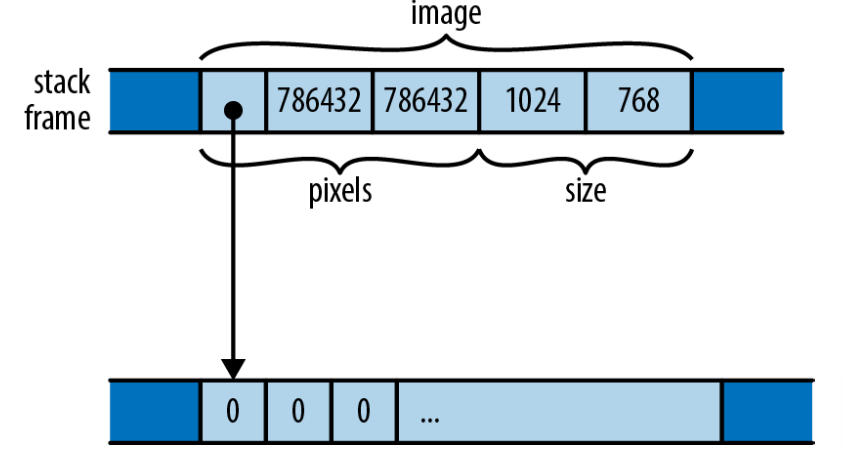
\includegraphics[width=0.8\textwidth]{../img/f9-1.png}
    \caption{一个\texttt{GrayscaleMap}结构体的内存布局}
    \label{f9-1}
\end{figure}

与C和C++不同，Rust对于如何在内存中布局结构体字段或元素没有任何确切的保证，这里的图只是展示了其中一种可能的排列。然而Rust确实保证了直接在结构体的内存块里存储字段的值。JavaScript、Python和Java将会把\texttt{pixels}和\texttt{size}值分别放在它们自己的堆上分配的内存块中，然后让\texttt{GrayscaleMap}的字段指向他们。而Rust会直接把\texttt{pixels}和\texttt{size}嵌入到\texttt{GrayscaleMap}值里。只有\texttt{pixels} vector持有的堆上分配的缓冲区保留着自己的块。

你可以使用\texttt{\#[repr(C)]}属性来要求Rust用一种与C和C++兼容的方式布局结构体。我们将会在\hyperref[ch23]{第23章}中详细介绍这些。

\section{使用\texttt{impl}定义方法}\label{method}

在本书中，我们已经在很多类型的值上调用过方法。我们使用\texttt{v.push(e)}把元素添加进vector，使用\texttt{v.len()}获取它的长度，使用\texttt{r.expect("msg")}检查\texttt{Result}的值是否是错误值，等等。你可以为你自己的结构体类型定义方法。与C++或Java那种直接出现在结构体定义内部的方式不同，Rust的方法在一个单独的\texttt{impl}块中定义。

一个\texttt{impl}块就是一些\texttt{fn}定义的结合，每一个函数都将成为这个结构体的一个方法。例如，这里我们定义了一个公有的结构体\texttt{Queue}，然后为它定义了两个公有的方法：\texttt{push}和\texttt{pop}：
\begin{minted}{Rust}
    /// 一个先进先出的字符队列
    pub struct Queue {
        older: Vec<char>,   // 旧的元素，越旧越靠后
        younger: Vec<char>  // 新的元素，越新越靠后
    }

    impl Queue {
        /// 将一个字符添加到队列的尾部。
        pub fn push(&mut self, c: char) {
            self.younger.push(c);
        }

        /// 移出队列最前端的元素，如果有字符被移出就返回`Some(c)`，
        /// 否则如果队列为空就返回`None`。
        pub fn pop(&mut self) -> Option<char> {
            if self.older.is_empty() {
                if self.younger.is_empty() {
                    return None;
                }

                // 将新的元素都移动到旧的元素里，
                // 并且反转顺序。
                use std::mem::swap;
                swap(&mut self.older, &mut self.younger);
                self.older.reverse();
            }

            // 现在旧的元素保证不为空。Vec的pop方法
            // 已经返回了一个Option，因此不用再处理
            self.older.pop()
        }
    }
\end{minted}

在\emph{impl}块中定义的函数被称为\emph{关联函数}，因为它们被关联到特定的类型。与之相反的是\emph{自由函数}，也就是不在\texttt{impl}块中定义的函数。

Rust将调用方法的值作为第一个参数传给方法，它的参数名必须是\texttt{self}。因为\texttt{self}的类型很明显是\texttt{impl}块外面的结构体类型，或者是其引用，所以Rust允许你省略类型，用\texttt{self}、\texttt{\&self}、\texttt{\&mut self}分别作为\texttt{self: Queue}、\texttt{self: \&Queue}、\texttt{self: \&mut Queue}的缩写。如果你喜欢的话也可以使用非缩写的形式，但几乎所有的Rust代码都是用缩写形式。

在我们的示例中，\texttt{push}和\texttt{pop}方法中通过\texttt{self.older}和\texttt{self.younger}引用了\texttt{Queue}的字段。与C++或Java中“this”对象的成员直接在方法内可见不同，Rust方法中必须显式使用\texttt{self}来引用字段，这和Python方法中\texttt{self}的用法、JavaScript方法中\texttt{this}的用法类似。

因为\texttt{push}和\texttt{pop}需要修改\texttt{Queue}，所以它们都以\texttt{\&mut self}传参。然而，当你调用这两个方法时，你不需要手动借用可变引用，普通的方法调用语法会自动进行隐式转换。因此有了这些定义之后，你可以像这样使用\texttt{Queue}：
\begin{minted}{Rust}
    let mut q = Queue { older: Vec::new(), younger: Vec::new() };

    q.push('0');
    q.push('1');
    assert_eq!(q.pop(), Some('0'));

    q.push('=');
    assert_eq!(q.pop(), Some('1'));
    assert_eq!(q.pop(), Some('='));
    assert_eq!(q.pop(), None);
\end{minted}

为了满足\texttt{push}方法的\texttt{self}参数要求，直接写\texttt{q.push(...)}会借用\texttt{q}的可变引用，就像你写了\texttt{(\&mut q).push(...)}一样。

如果一个方法不需要修改\texttt{self}，那么你可以以共享引用获取参数。例如：
\begin{minted}{Rust}
    impl Queue {
        pub fn is_empty(&self) -> bool {
            self.older.is_empty() && self.younger.is_empty()
        }
    }
\end{minted}

方法调用表达式知道要借用哪一种引用：
\begin{minted}{Rust}
    assert!(q.is_empty());
    q.push('☉');
    assert!(!q.is_empty());
\end{minted}

或者，如果一个方法想获取\texttt{self}的所有权，它可以以值传递\texttt{self}：
\begin{minted}{Rust}
    impl Queue {
        pub fn split(self) -> (Vec<char>, Vec<char>) {
            (self.older, self.younger)
        }
    }
\end{minted}

调用这个\texttt{split}方法看起来和调用其他方法一样：
\begin{minted}{Rust}
    let mut q = Queue { older: Vec::new(), younger: Vec::new() };

    q.push('P');
    q.push('D');
    assert_eq!(q.pop(), Some('P'));
    q.push('X');

    let (older, younger) = q.split();
    // q现在是未初始化状态
    assert_eq!(older, vec!['D']);
    assert_eq!(younger, vec!['X']);
\end{minted}

但是注意，因为\texttt{split}以值获取\texttt{self}，这会把\texttt{q}中的\texttt{Queue}值\emph{移动}走，导致\texttt{q}变为未初始化。因为\texttt{split}的\texttt{self}现在拥有了这个队列，因此它可以把两个单独的vector移动出来并返回给调用者。

有时，像这样以值传递\texttt{self}，或者以引用传递都不能满足我们的需求，因此Rust还允许你通过智能指针类型传递\texttt{self}。

\subsection{以\texttt{Box}、\texttt{Rc}、\texttt{Arc}传递\texttt{Self}}

一个方法的\texttt{self}参数还可以是\texttt{Box<Self>}、\texttt{Rc<Self>}、\texttt{Arc<Self>}。这些方法只能在相应指针类型上调用。调用这些方法会传递指针的所有权。

你通常不需要这么做。一个以引用传递\texttt{self}的方法可以在任何智能指针类型上正常调用：
\begin{minted}{Rust}
    let mut bq = Box::new(Queue::new());

    // `Queue::push`接受一个`&mut Queue`，但`bq`是`Box<Queue>`。
    // 这没有问题：Rust在调用期间从`Box`借用了一个`&mut Queue`
    bq.push('■');
\end{minted}

对于方法调用和字段访问，Rust自动从智能指针类型例如\texttt{Box}、\texttt{Rc}和\texttt{Arc}借用一个引用，因此\texttt{\&self}和\texttt{\&mut self}通常总是正确的方法签名，再加上偶尔用到的\texttt{self}。

但如果这个方法的意图涉及管理指针的所有权呢？假设我们有一个像这样的节点组成的树，类似某种彻底简化的XML：
\begin{minted}{Rust}
    use std::rc::Rc;

    struct Node {
        tag: String,
        children: Vec<Rc<Node>>
    }

    impl Node {
        fn new(tag: &str) -> Node {
            Node {
                tag: tag.to_string(),
                children: vec![],
            }
        }
    }
\end{minted}

每一个节点都有一个tag来指示它是什么类型的节点，还有一个子节点的vector通过引用计数指针来允许共享，并让生命周期变得更灵活。

通常我们会实现一个方法让它向自己的列表中添加一个子节点，但现在让我们把角色颠倒过来，给\texttt{Node}实现一个把它自己添加到别的\texttt{Node}的子节点中的方法。我们可以写：
\begin{minted}{Rust}
    impl Node {
        fn append(self, parent: &mut Node) {
            parent.children.push(Rc::new(self));
        }
    }
\end{minted}

但这个方法并不能让人满意。这个方法调用了\texttt{Rc::new}来分配新的堆空间并且把\texttt{self}移动进去，但如果调用者已经有了一个\texttt{Rc<Node>}，这些操作就都不是必须的：我们应该只递增引用计数然后把指针加到vector里。\texttt{Rc}的全部意义不就是实现共享吗？

我们可以这样写：
\begin{minted}{Rust}
    impl Node {
        fn append_to(self: Rc<Self>, parent: &mut Node) {
            parent.children.push(self);
        }
    }
\end{minted}

如果调用者已经是\texttt{Rc<Node>}类型，那它可以直接调用\texttt{append\_to}，以值传递\texttt{Rc}：
\begin{minted}{Rust}
    let shared_node = Rc::new(Node::new("first"));
    shared_node.append_to(&mut parent);
\end{minted}

这会把\texttt{shared\_node}的所有权传递给方法：引用计数不会发生变化，也不会有新的内存分配。

如果调用者需要保留节点的指针以便之后使用，它可以首先克隆\texttt{Rc}再调用：
\begin{minted}{Rust}
    shared_node.clone().append_to(&mut parent);
\end{minted}

克隆\texttt{Rc}只会递增引用计数，没有堆分配或者拷贝。但当调用返回时\texttt{shared\_node}和\texttt{parent}\\
的子节点的vector现在指向同一个\texttt{Node}。

最后，如果调用者现在拥有一个\texttt{Node}，那么它必须先创建一个\texttt{Rc}再调用方法：
\begin{minted}{Rust}
    let owned = Node::new("owned directly");
    Rc::new(owned).append_to(&mut parent);
\end{minted}

把\texttt{append\_to}方法的签名设为\texttt{Rc<Self>}可以让调用者知道\texttt{Node}的需求。然后调用者可以用最小化内存分配和引用计数调整的方式来调用：
\begin{itemize}
    \item 如果可以传递\texttt{Rc}的所有权，就直接在指针上调用。
    \item 如果需要保留\texttt{Rc}的所有权，就递增引用计数后再调用。
    \item 如果只拥有\texttt{Node}，那么必须先调用\texttt{Rc::new}来分配堆空间然后把\texttt{Node}移动进去。因为\texttt{parent}必须通过\texttt{Rc<Node>}指针引用它的子节点，所以这一步最终肯定是必须的。
\end{itemize}

再重复一遍，对于大多数方法，\texttt{\&self}、\texttt{\&mut self}、和\texttt{self}（以值传参）就能满足你的需求。但如果一个方法的目的是影响值的所有权，使用其他指针类型的\texttt{self}可能是正确的选择。

\subsection{类型关联函数}
\texttt{impl}块里定义的函数也可以没有\texttt{self}参数。这些参数仍然和类型关联，因为它们也是在\texttt{impl}块中定义的。但它们不是方法，因为它们没有\texttt{self}参数。为了将它们和方法区别开来，我们称它们为\emph{类型关联函数}。

它们通常用于提供构造函数，例如：
\begin{minted}{Rust}
    impl Queue {
        pub fn new() -> Queue {
            Queue { older: Vec::new(), younger: Vec::new() }
        }
    }
\end{minted}

为了使用这个函数，我们通过\texttt{Queue::new}来引用它：类型名+双冒号+函数名。现在我们的示例代码变得更加简洁：
\begin{minted}{Rust}
    let mut q = Queue::new();

    q.push('*');
    ...
\end{minted}

Rust的传统是构造函数都叫\texttt{new}，我们已经见过了\texttt{Vec::new}、\texttt{Box::new}、\texttt{HashMap::new}，等等。但\texttt{new}这个名字本身并没有什么特殊的地方。它并不是关键字，而且一个类型经常还有其他名字的关联函数作为构造函数，例如\texttt{Vec::with\_capacity}。

尽管一个类型可以有很多个分开的\texttt{impl}块，但它们必须在定义类型的那个crate中。然而，Rust确实允许你将自己定义的方法附加到其他类型，我们将在\hyperref[ch11]{第11章}介绍怎么做到这一点。

如果你习惯写C++或Java，你可能会觉得将类型的方法和定义分离开来很奇怪，但这么做确实有以下优势：
\begin{itemize}
    \item 你总是能很容易的找到一个类型的数据成员。在很大的C++类定义中，你可能需要浏览几百行成员成员函数的定义来确保你没有遗漏数据成员。而在Rust中，所有数据成员都在一个地方。
    \item 尽管我们可以很容易想象把方法定义添加到命名字段结构体的定义中，但类元组结构体和类单元结构体却不是这样。将方法拿出来放在一个\texttt{impl}块中可以让这三种结构体共用唯一一种语法。事实上，Rust还使用这套语法为不是结构体的类型定义方法，例如\texttt{enum}结构体和基本类型例如\texttt{i32}。（任何类型都可以有方法的事实是Rust中不使用术语\emph{对象}，而是更喜欢把一切称为\emph{值}的原因之一。）
    \item 同样的\texttt{impl}语法还可以很容易地用于实现trait，我们将在\hyperref[ch11]{第11章}中介绍。
\end{itemize}

\section{关联常量}
Rust的类型系统还采用了C\#和Java等语言中的一个特性，就是关联到类型而不是关联到类型实例的值。在Rust中，它们被称为\emph{关联常量}。

正如它的名字一样，关联常量是常量值。它们通常用来表示某一个类型中使用最广泛的值。例如，你可以定义一个二维的向量用于线性代数，并为它定义一个关联的单位向量：
\begin{minted}{Rust}
    pub struct Vector2 {
        x: f32,
        y: f32,
    }

    impl Vector2 {
        const ZERO: Vector2 = Vector2 { x: 0.0, y: 0.0 };
        const UNIT: Vector2 = Vector2 { x: 1.0, y: 0.0 };
    }
\end{minted}

这些值被关联到类型本身，你可以在不创建\texttt{Vector2}的实例的情况下使用它们。和类型关联方法一样，引用它们的方法是类型的名称再加上它们的名称：
\begin{minted}{Rust}
    let scaled = Vector2::UNIT.scaled_by(2.0);
\end{minted}

关联常量的类型并不一定必须是它关联的类型，我们可以使用这个特性来给类型添加ID或者名称。例如，如果有几个和\texttt{Vector2}很像的类型需要写入到文件里，然后加载到内存中，那么关联常量可以为写入的数据添加名称或数字ID，这样之后可以据此辨识出类型：
\begin{minted}{Rust}
    impl Vector2 {
        const NAME: &'static str = "Vector2";
        const ID: u32 = 18;
    }
\end{minted}

\section{泛型结构体}\label{GenStruct}

我们之前的\texttt{Queue}定义并不能令人满意：它被用来存储字符，但它却没有任何和字符相关的方法。如果我们要定义另一个存储\texttt{String}值的结构体，那么除了\texttt{char}要换成\texttt{String}之外，剩下的代码完全相同。重复定义将会浪费时间。

幸运的是，Rust的结构体可以是\emph{泛型}的，这意味着它们的定义只是一个模板，你可以把任何类型塞进去。例如，这里有一个可以存储任何类型的值的\texttt{Queue}的定义：
\begin{minted}{Rust}
    pub struct Queue<T> {
        older: Vec<T>,
        younger: Vec<T>
    }
\end{minted}

你可以将\texttt{Queue<T>}中的\texttt{<T>}读作“对于任意类型\texttt{T}”。因此这个定义读作“对于任意类型\texttt{T}，一个\texttt{Queue<T>}有两个\texttt{Vec<T>}类型的字段。”例如，在\texttt{Queue<String>}中，\texttt{T}是\texttt{String}，所以\texttt{older}和\texttt{younger}的类型都是\texttt{Vec<String>}。在\texttt{Queue<char>}中\texttt{T}是\texttt{char}，我们就得到了一个和一开始的\texttt{char}类型特定的定义完全相同的结构体。事实上，\texttt{Vec}本身就是一个用这种方式定义的泛型结构体。

在泛型结构体的定义中，<尖括号>里的类型名被称为\emph{类型参数}。一个泛型结构体的\texttt{impl}块看起来像这样：
\begin{minted}{Rust}
    impl<T> Queue<T> {
        pub fn new() -> Queue<T> {
            Queue { older: Vec::new(), younger: Vec::new() }
        }

        pub fn push(&mut self, t: T) {
            self.younger.push(t);
        }

        pub fn is_empty(&self) -> bool {
            self.older.is_empty() && self.younger.is_empty()
        }

        ...
    }
\end{minted}

你可以将\texttt{impl<T> Queue<T>}这一行读作“对于任意类型\texttt{T}，有一些\texttt{Queue<T>}可用的关联方法”。然后，你可以在关联函数的定义中将类型参数\texttt{T}用作一个类型。

这种语法看起来好像有些重复，但\texttt{impl<T>}能更清晰地表达出\texttt{impl}块覆盖了任意的类型\texttt{T}，这能将它和为特定种类的\texttt{Queue}编写的\texttt{impl}块区分开来，例如：
\begin{minted}{Rust}
    impl Queue<f64> {
        fn sum(&self) -> f64 {
            ...
        }
    }
\end{minted}

这个\texttt{impl}块头读作“这里有一些\texttt{Queue<f64>}特定的关联方法”。这样就给\texttt{Queue<f64>}添加了一个\texttt{sum}方法，而其它种类的\texttt{Queue}并没有这个方法。

我们已经在之前的代码中使用过Rust的\texttt{self}参数的缩写形式。这里\texttt{Queue<T>}如果写出类型显得有些啰嗦。作为另一种缩写，每一个\texttt{impl}块，不管是不是泛型的，都定义了特殊的类型参数\texttt{Self}（注意\texttt{大驼峰}风格的名称）来表示我们要添加方法的类型。在之前的代码中，\texttt{Self}将是\texttt{Queue<T>}，因此我们可以进一步简化\texttt{Queue::new}的定义：
\begin{minted}{Rust}
    pub fn new() -> Self {
        Queue { older: Vec::new(), younger: Vec::new() }
    }
\end{minted}

你可能已经注意到了，在\texttt{new}的函数体内，我们不需要在构造表达式中写出类型参数，简单地写\texttt{Queue \{ ... \}}就足够了。这是因为Rust的类型推导发挥了作用：因为函数的返回值类型只能有一种可能，就是\texttt{Queue<T>}，所以Rust会自动为我们提供参数。然而，你必须总是在函数签名和类型定义中指明类型参数。Rust不会推断它们，相反，它将这些已知的类型作为基础来推断那些函数体内的类型。

\texttt{Self}也可以用于这种方式：我们可以写\texttt{Self \{ ... \}}。你觉得哪种形式更容易理解就可以用哪种。

对于关联函数的调用，你可以显式地使用\texttt{::<>(涡轮鱼)}注解来提供类型参数：
\begin{minted}{Rust}
    let mut q = Queue::<char>::new();
\end{minted}

但在实践中，通常可以让Rust自动帮你推断类型：
\begin{minted}{Rust}
    let mut q = Queue::new();
    let mut r = Queue::new();

    q.push("CAD");      // 显然是Queue<&'static str>
    r.push(0.74);       // 显然是Queue<f64>

    q.push("BTC");      // 比特币/USD，2019年6月 
    r.push(13764.0);    
\end{minted}

事实上，这正是整本书中我们使用\texttt{Vec}的方式。

并不只有结构体可以是泛型的。枚举也可以有类型参数，语法也非常的相似。我们将在\nameref{enum}一节中详细介绍。

\section{有生命周期参数的结构体}

正如我们在\nameref{refstruct}一节中讨论过的一样，如果一个结构体类型中包含引用，你必须指明那些引用的生命周期。例如，这里有一个存储切片中最大和最小元素的引用的结构体：
\begin{minted}{Rust}
    struct Extrema<'elt> {
        greatest: &'elt i32,
        least: &'elt i32
    }
\end{minted}

之前，我们建议你将类似\texttt{struct Queue<T>}的声明看作是对于任意类型\texttt{T}，你都可以构建一个\texttt{Queue<T>}来存储该类型。类似的，你可以将\texttt{struct Extrema<'elt>}看作对于任意生命周期\texttt{'elt}，你都可以构建一个\texttt{Extrema<'elt>}来存储生命周期为\texttt{'elt}的引用。

这里有一个函数来扫描一个切片并返回一个指向其中元素的\texttt{Extrema}值：
\begin{minted}{Rust}
    fn find_extrema<'s>(slice: &'s [i32]) -> Extrema<'s> {
        let mut greatest = &slice[0];
        let mut least = &slice[0];

        for i in 1..slice.len() {
            if slice[i] < *least    { least     = &slice[i]; }
            if slice[i] > *greatest { greatest  = &slice[i]; }
        }
        Extrema { greatest, least }
    }
\end{minted}

这里，\texttt{find\_extrema}借用了\texttt{slice}的元素。因为\texttt{slice}的生命周期是\texttt{'s}，所以我们返回的\texttt{Extrema}结构体中的引用的生命周期也是\texttt{'s}。Rust总是会为调用推断生命周期参数，因此调用\texttt{find\_extrema}并不需要提到它们：
\begin{minted}{Rust}
    let a = [0, -3, 0, 15, 48];
    let e = find_extrema(&a);
    assert_eq!(*e.least, -3);
    assert_eq!(*e.greatest, 48);
\end{minted}

因为返回值和参数使用相同的生命周期非常常见，所以当只有一种可能时Rust允许我们省略生命周期。我们还可以在不改变含义的情况下将\texttt{find\_extrema}的签名写成这样：
\begin{minted}{Rust}
    fn find_extrema(slice: &[i32]) -> Extrema {
        ...
    }
\end{minted}

诚然，我们也\emph{可能}是想返回\texttt{Extrema<'static>}，但这并不是通常的情况。Rust只为通常的情况提供了一个缩写。

\section{为结构体类型派生常见的trait}

可以非常简单地定义一个结构体：
\begin{minted}{Rust}
    struct Point {
        x: f64,
        y: f64
    }
\end{minted}

然而，如果你真的开始使用这个\texttt{Point}类型，你将很快发现它使用起来很痛苦。按照上面的写法，\texttt{Point}既不能拷贝也不能克隆。你不能用\texttt{println!("\{:?\}", point);}打印它，它也不支持\texttt{==}和\texttt{!=}运算符。

在Rust中这些特性都有一个名字——\texttt{Copy}、\texttt{Clone}、\texttt{Debug}、\texttt{PartialEq}。它们被称为\emph{trait}。在\hyperref[ch11]{第11章}中，我们将展示如何为你自己的结构体手动实现trait。但这个例子中出现的标准trait，以及其它一些trait，你不需要手动实现它们，除非你想要一些自定义行为。Rust可以自动为你实现它们。只需要为结构体添加\texttt{\#[derive]}属性：
\begin{minted}{Rust}
    #[derive(Copy, Clone, Debug, PartialEq)]
    struct Point {
        x: f64,
        y: f64
    }
\end{minted}

这些trait中的任何一个都可以自动实现，前提是这个结构体的所有字段都实现了那个trait。我们可以要求Rust为\texttt{Point}派生\texttt{PartialEq}，是因为它的两个字段都是\texttt{f64}类型，这个类型已经实现了\texttt{PartialEq}。

Rust还可以派生\texttt{PartialOrd}，它可以支持比较运算符\texttt{<}、\texttt{>}、\texttt{<=}和\texttt{>=}。我们没有这么做，是因为比较两个点来判断其中一个是否“小于”另一个是一件很奇怪的事。因此我们选择让\texttt{Point}值不支持那些比较运算符。像这样的情况也是Rust让我们自己写\texttt{\#[derive]}属性而不是直接自动派生所有可用的trait的原因之一。另一个原因是实现一个trait将自动变为公有的特性。因此可复制性、可克隆性等都将是结构体公共API的一部分，应该慎重选择。

我们将在\hyperref[ch13]{第13章}详细介绍Rust的标准trait并解释哪些可以用\texttt{\#[derive]}自动实现。

\section{内部可变性}\label{intermut}

可变性和其他东西一样：如果限制太过宽松就会导致问题，但你又总是希望它能放宽一点。例如，假设你的蜘蛛机器人控制系统是一个中心化的结构体\texttt{SpiderRobot}，这个结构体里包含设置和I/O处理。当机器人启动时它的值就被初始化，并且永远不会改变：
\begin{minted}{Rust}
    pub struct SpiderRobot {
        species: String,
        web_enabled: bool,
        leg_devices: [fd::FileDesc; 8],
        ...
    }
\end{minted}

机器人的每一个主要系统都由一个不同的结构体处理，这些结构体都有一个指向那个\texttt{SpiderRobot}值的指针：
\begin{minted}{Rust}
    use std::rc::Rc;

    pub struct SpiderSenses {
        robot: Rc<SpiderRobot>, // <-- 指向设置和I/O的指针
        eyes: [Camera; 32],
        motion: Accelerometer,
        ...
    }
\end{minted}

控制织网、捕食、毒液流动等的结构体都有一个\texttt{Rc<SpiderRobot>}智能指针。回顾一下，\texttt{Rc}代表\hyperref[rc]{引用计数},、\texttt{Rc}中的值总是共享的因此总是不可变的。

现在假设你想使用标准的\texttt{File}类型给\texttt{SpiderRobot}结构体添加一点日志功能。那么就会有一个问题：\texttt{File}值必须是\texttt{mut}的。所有写入它的函数都需要\texttt{mut}引用。

这种情况经常出现。我们需要的是一个不可变(\texttt{SpiderRobot}结构体)的值内有一小部分数据可变(一个\texttt{File})。这被称为\emph{内部可变性}。Rust为此提供了几种方式，这一节中我们将讨论最直观的两种类型：
\texttt{Cell<T>}和\texttt{RefCell<T>}，这两个类型都在\texttt{std::cell}模块中。

\texttt{Cell<T>}结构体只包含单个私有的类型\texttt{T}的值。\texttt{Cell}唯一特殊的地方是即使你没有对\texttt{Cell}自身的\texttt{mut}访问权限，也可以访问和修改它里面的字段值：

\codeentry{Cell:new(value)}
\hangparagraph{创建一个新的\texttt{Cell}，将给定的\texttt{value}移动进去。}

\codeentry{cell.get()}
\hangparagraph{返回一个\texttt{cell}中值的拷贝}

\codeentry{cell.set(value)}
\hangparagraph{将给定的值\texttt{value}存储在\texttt{cell}中，丢弃掉之前存储的值。这个方法以非\texttt{mut}引用获取\texttt{self}参数：}
\begin{minted}{Rust}
    fn set(&self, value: T) // 注意：不是`&mut self`
\end{minted}
\hangparagraph{显然，这和普通的\texttt{set}方法不同。到目前为止，Rust告诉我们如果想要修改数据就需要\texttt{mut}访问权限。但同样的道理，这一处不同的细节就是\texttt{Cell}全部的精髓。它们是一种安全地扭曲不可变性规则的方式——既不多、也不少。}

\texttt{Cell}还可以有一些其他的方法，你可以在\href{https://doc.rust-lang.org/std/cell/struct.Cell.html}{它的文档}中查阅。

如果你想给你的\texttt{SpiderRobot}添加一个简单的计数器，那么使用\texttt{Cell}将会很方便。你可以写：
\begin{minted}{Rust}
    use std::cell::Cell;

    pub struct SpiderRobot {
        ...
        hardware_error_count: Cell<u32>,
        ...
    }
\end{minted}

即使是\texttt{SpiderRobot}的非\texttt{mut}方法也可以使用\texttt{.get()}和\texttt{.set()}来访问\texttt{u32}：
\begin{minted}{Rust}
    impl SpiderRobot {
        /// 错误计数加一
        pub fn add_hardware_error(&self) {
            let n = self.hardware_error_count.get();
            self.hardware_error_count.set(n + 1);
        }

        /// 如果有硬件错误的话返回真
        pub fn has_hardware_errors(&self) -> bool {
            self.hardware_error_count.get() > 0
        }
    }
\end{minted}

这非常简单，但并不能解决我们的日志问题。\texttt{Cell}\emph{不能}让你调用内含值的\texttt{mut}方法，因为\texttt{.get()}方法返回的是单元里值的拷贝，所以它只能用于实现了\hyperref[copy]{\texttt{Copy} trait}的类型。为了实现日志功能，我们需要一个可变的\texttt{File}，而\hyperref[file]{\texttt{File}}不可拷贝。

这个例子中正确的工具是\texttt{RefCell}。类似于\texttt{Cell<T>}，\texttt{RefCell<T>}也是一个包含单个\texttt{T}类型的值的泛型类型。和\texttt{Cell}不同的是，\texttt{RefCell}支持借用内部的\texttt{T}类型的值：

\codeentry{RefCell::new(value)}
\hangparagraph{创建一个新的\texttt{RefCell}，把\texttt{value}移动进去。}

\codeentry{ref\_cell.borrow()}
\hangparagraph{返回一个\texttt{Ref<T>}，它本质上是\texttt{ref\_cell}里存储的值的一个共享引用。}
\hangparagraph{如果里面的值已经有可变借用了，这个方法会panic。}

\codeentry{ref\_cell.borrow\_mut()}
\hangparagraph{返回一个\texttt{RefMut<T>}，它本质上是\texttt{ref\_cell}里存储的值的一个可变引用。}
\hangparagraph{如果里面的值已经被借用了，这个方法会panic。}

\codeentry{ref\_cell.try\_borrow(), ref\_cell.try\_borrow\_mut()}
\hangparagraph{与\texttt{borrow()}和\texttt{borrow\_mut()}的功能一样，但返回一个\texttt{Result}。当值已经有可变借用/被借用时，它们不panic，而是返回一个\texttt{Err}值。}

同样的，\texttt{RefCell}还有一些其它方法，你可以在\href{https://doc.rust-lang.org/std/cell/struct.RefCell.html}{它的文档}中查阅。

只有当你尝试打破Rust中\texttt{mut}引用必须是独占引用的规则时这两个方法才会panic。例如，这样将会panic：
\begin{minted}{Rust}
    use std::cell::RefCell;

    let ref_cell: RefCell<String> = RefCell::new("hello".to_string());

    let r = ref_cell.borrow();  // ok，返回一个Ref<String>
    let count = r.len();        // ok, 返回"hello".len()
    assert_eq!(count, 5);       

    let mut w = ref_cell.borrow_mut(); // panic：已经被借用了
    w.push_str(" world");
\end{minted}

为了避免panic，你可以把这两个借用放进单独的块里。这样的话，\texttt{r}会在你尝试借用\texttt{w}之前被drop。

这和普通引用的工作方式很像。唯一的不同在于普通的情况下，当你尝试借用一个变量的引用，Rust会在\emph{编译期}确保你必须安全地使用引用。如果检查失败了，你会得到一个编译期错误。\texttt{RefCell}使用运行时检查来执行同样的规则。如果你尝试打破规则，你会得到一个panic（或者使用\texttt{try\_borrow}和\texttt{try\_borrow\_mut}时会得到一个\texttt{Err}）。

现在我们已经准备好用\texttt{RefCell}来完善我们的\texttt{SpiderRobot}了：
\begin{minted}{Rust}
    pub struct SpiderRobot {
        ...
        log_file: RefCell<File>,
        ...
    }

    impl SpiderRobot {
        /// 向日志文件中写入一行。
        pub fn log(&self, message: &str) {
            let mut file = self.log_file.borrow_mut();
            // `writeln!`和`println!`很像，
            // 但会把字符串写入到给定的文件中。
            writeln!(file, "{}", message).unwrap();
        }
    }
\end{minted}

变量\texttt{file}的类型是\texttt{RefMut<File>}。它的使用方式就像\texttt{File}的可变引用一样。有关写入文件的细节，见\hyperref[ch18]{第18章}。

Cell很容易使用。虽然必须调用\texttt{.get()}和\texttt{.set()}或者\texttt{.borrow()}和\texttt{.borrow\_mut()}有点麻烦，但那只是我们扭曲可变性规则的代价。还有一些不是很明显但却更严重的问题：Cell——和任何包含了它们的类型——都不是线程安全的。因此Rust\hyperref[threadsafe]{不允许}多个线程直接访问它们。我们将在\hyperref[ch19]{第19章}中讨论到\nameref{mutex}、\nameref{atomic}和\nameref{globalvar}时介绍多线程中的内部可变性。

不管一个结构体有命名字段还是类元组结构体，它都是一些其他值的聚合体：如果我有一个\texttt{SpiderSenses}结构体，那么我就有一个指向共享的\texttt{SpiderRobot}结构体的\texttt{Rc}指针、同时还有了eyes、accelerometer等等。因此结构体的本质是单词“和(and)”：我有一个X \emph{和(and)} 一个Y。但是否有另一种类型用于单词“或(or)”呢？换句话说，当你有了一个这种类型的值时，你有了一个X \emph{或(or)} 一个Y？这样的类型太有用了以至于它们在Rust中无处不在，它们就是我们下一章要讨论的主题。

\chapter{枚举与模式}\label{ch10}

\emph{Surprising how much computer stuff makes sense viewed as tragic deprivation of sum types (cf. deprivation of lambdas).}

\begin{flushright}
    ——Graydon Hoare
\end{flushright}

这一章的第一个话题将是一个古老的、强有力的、可以帮你在短期内完成很多工作的（有代价地）、并且在许多语言中以不同的名字广为人知的特性。但它并不是魔鬼。而是一种用户自定义的数据类型，它是ML和Haskell程序员们熟知的和类型、也是互斥的联合、还是代数数据类型。在Rust中，它们被称为\emph{枚举(enumerations)}，或者简写为\emph{enum}。和魔鬼不同的是，它们非常安全、索取的代价也很小。

C++和C\#都有枚举，你可以使用它们来定义自己的类型，这种类型的取值范围是一些命名常量的集合。例如，你可能定义过一个叫\texttt{Color}的类型，取值范围为\texttt{Red}、\texttt{Orange}、\texttt{Yellow}等等。这种枚举在Rust中也能工作，但Rust进一步扩展了枚举。一个Rust枚举可以包含数据，包括多种不同类型的数据。例如，Rust的\texttt{Result<String, io::Error}类型是一个枚举；这样一个值要么是一个包含\texttt{String}的\texttt{Ok}值要么是一个包含\texttt{io::Error}的\texttt{Err}值。这就超出了C++和C\#中枚举的能力。它更像C中的\texttt{union}——但和联合不同的是，Rust的枚举是类型安全的。

枚举适用于一个值有多种可能的情况。使用它们的“代价”是你必须使用模式匹配来安全地访问数据，这也是我们这一章中的第二个话题。

如果你使用过Python的解包或者JavaScript中的解构，那你可能觉得模式也很熟悉，但Rust同样扩展了模式。Rust的模式有点像匹配数据的正则表达式。它们被用来测试一个值是否具有特定的期望的形态。它们可以一次从结构体或这元组中提取出多个字段存入局部变量。并且和正则表达式类似，它们很简洁，通常只用单行代码就能完成任务。

这一章将以枚举的基础开始，展示数据怎么被关联到枚举选项以及枚举是怎么存储在内存中的。然后我们会展示Rust的模式和\texttt{match}表达式如何简洁地指定基于枚举、结构体、数组、切片的逻辑。模式也可以包含引用、move和\texttt{if}条件，这让它们的功能更加强大。

\section{枚举}\label{enum}

简单的C风格枚举非常直观：
\begin{minted}{Rust}
    enum Ordering {
        Less,
        Equal,
        Greater,
    }
\end{minted}

这里声明了一个有三个可能的值的\texttt{Ordering}类型，这些值被称为\emph{variant}或者\emph{constructor}：\texttt{Ordering::Less}、\texttt{Ordering::Equal}、\texttt{Ordering::Greater}。这个枚举是标准库的一部分，因此Rust代码可以导入它：
\begin{minted}{Rust}
    use std::cmp::Ordering;

    fn compare(n: i32, m: i32) -> Ordering {
        if n < m {
            Ordering::Less
        } else if n > m {
            Ordering::Greater
        } else {
            Ordering::Equal
        }
    }
\end{minted}

或者它的所有constructor：
\begin{minted}{Rust}
    use std::cmp::Ordering::{self, *};  // `*`意思是导入所有的子item

    fn compare(n: i32, m: i32) -> Ordering {
        if n < m {
            Less
        } else if n > m {
            Greater
        } else {
            Equal
        }
    }
\end{minted}

导入constructor之后，我们可以写\texttt{Less}来代替\texttt{Ordering::Less}等，但因为这样不够明显，因此一般认为\emph{不要}导入它们式更好的风格，除非它能是你的代码的可读性更强。

为了导入一个在当前模块中声明的枚举的constructor，可以使用\texttt{self}：
\begin{minted}{Rust}
    enum Pet {
        Orca,
        Giraffe,
        ...
    }

    use self::Pet::*;
\end{minted}

在内存中，C风格的枚举值被存储为整数。有时告诉Rust使用哪些整数会很有用：
\begin{minted}{Rust}
    enum HttpStatus {
        Ok = 200,
        NotModified = 304,
        NotFound = 404,
        ...
    }
\end{minted}

否则，Rust会从0开始自动分配值。

默认情况下，Rust用能容纳所有值的最小的内建整数类型来存储C风格枚举。大多数情况下都是一个单独的字节：
\begin{minted}{Rust}
    use std::mem::size_of;
    assert_eq!(size_of::<Ordering>(), 1);
    assert_eq!(size_of::<HttpStatus>(), 2); // 404不能存储在u8中
\end{minted}

你可以通过添加\texttt{\#[repr]}属性来覆盖Rust选择的内存表示方式。更多的细节见“\nameref{repr}”。

将C风格的枚举转换为整数是允许的：
\begin{minted}{Rust}
    assert_eq!(HttpStatus::Ok as i32, 200);
\end{minted}

然而，反过来把整数转换为枚举是不允许的。和C和C++不同，Rust保证枚举的值只能是\texttt{enum}生命中列出的值之一。未经检查的从整数类型到枚举类型的转换会打破这种保证，所以它是不允许的。你可以写出你自己的带检查的版本：
\begin{minted}{Rust}
    fn http_status_from_u32(n: u32) -> Option<HttpStatus> {
        match n {
            200 => Some(HttpStatus::Ok),
            304 => Some(HttpStatus::NotModified),
            404 => Some(HttpStatus::NotFound),
            ...
            _ => None,
        }
    }
\end{minted}

或者使用\href{https://crates.io/crates/enum_primitive}{\texttt{enum\_primitive}} crate。它包含一个宏可以为你自动生成这种类型的转换代码。

和结构体一样，编译器也可以为你自动生成类似\texttt{==}运算符这样的特性，但你需要显式地要求这样：
\begin{minted}{Rust}
    #[derive(Copy, Clone, Debug, PartialEq, Eq)]
    enum TimeUnit {
        Seconds, Minutes, Hours, Days, Months, Years,
    }
\end{minted}

枚举也和结构体一样可以拥有方法：
\begin{minted}{Rust}
    impl TimeUnit {
        /// 返回该时间单位的复数名词。
        fn plural(self) -> &'static str {
            match self {
                TimeUnit::Seconds => "seconds",
                TimeUnit::Minutes => "minutes",
                TimeUnit::Hours => "hours",
                TimeUnit::Days => "days",
                TimeUnit::Months => "months",
                TimeUnit::Years => "years",
            }
        }

        /// 返回该时间单位的单数名词。
        fn singular(self) -> &'static str {
            self.plural().trim_end_matches('s')
        }
    }
\end{minted}

C风格的枚举就这么多内容了。Rust中最有趣的一类枚举是那些带有数据的枚举。我们将展示这些枚举如何存储在内存中、如何通过添加类型参数将它们变为泛型的，以及如何通过枚举构建复杂的数据结构。

\subsection{带有数据的枚举}

一些程序总是需要显示完整的日期和时间，并且精确到毫秒。但对于大多数程序，显示大概的时间范围会更加友好，例如“两个月以前”。我们可以用之前定义的枚举编写一个新的枚举来实现这一点：
\begin{minted}{Rust}
    /// 一个故意舍入的时间戳，因此我们的程序会显示“6个月以前”
    /// 而不是“February 9, 2016, at 9:49 AM”。
    #[derive(Copy, Clone, Debug, PartialEq)]
    enum RoughTime {
        InThePast(TimeUnit, u32),
        JustNow,
        InTheFuture(TimeUnit, u32),
    }
\end{minted}

这个枚举中的两个variant，即\texttt{InThePast}和\texttt{InTheFuture}都有参数。这些被称为\emph{tuple variant}。就像类元组结构体一样，它们的constructor是创建新的\texttt{RoughTime}值的函数：
\begin{minted}{Rust}
    let four_score_and_seven_years_ago =
        RoughTime::InThePast(TimeUnit::Years, 4 * 20 + 7);

    let three_hours_from_now =
        RoughTime::InTheFuture(TimeUnit::Hours, 3);
\end{minted}

枚举也可以有\emph{struct variant}，它们和普通的结构体一样拥有命名字段：
\begin{minted}{Rust}
    enum Shape {
        Sphere { center: Point3d, radius: f32 },
        Cuboid { corner1: Point3d, corner2: Point3d },
    }

    let unit_sphere = Shape::Sphere {
        center: ORIGIN,
        radius: 1.0,
    };
\end{minted}

总的来说，Rust有三种枚举variant，分别对应我们在上一章中展示的三种结构体。没有数据的variant对应类单元结构体。元组variant对应类元组结构体。结构体variant对应有花括号和命名字段的结构体。一个枚举可以同时有这三种variant：
\begin{minted}{Rust}
    enum RelationshipStatus {
        Single,
        InARelationship,
        ItsComplicated(Option<String>),
        ItsExtremelyComplicated {
            car: DifferentialEquation, 
            cdr: EarlyModernistPoem,
        },
    }
\end{minted}

所有种类的constructor都和枚举自身有相同的可见性。

\subsection{内存中的枚举}

在内存中，带有数据的枚举被存储为一个很小的整数\emph{标签(tag)}，加上一块足够存储所有variant中最大的那个的内存。标签字段是Rust内部要使用的，它表示是哪一个constructor创建了这个值，进而得知这个值有哪些字段。

在Rust 1.50中，\texttt{RoughTime}存储为8个字节，如\hyperref[f10-1]{图10-1}所示。

\begin{figure}[htbp]
    \centering
    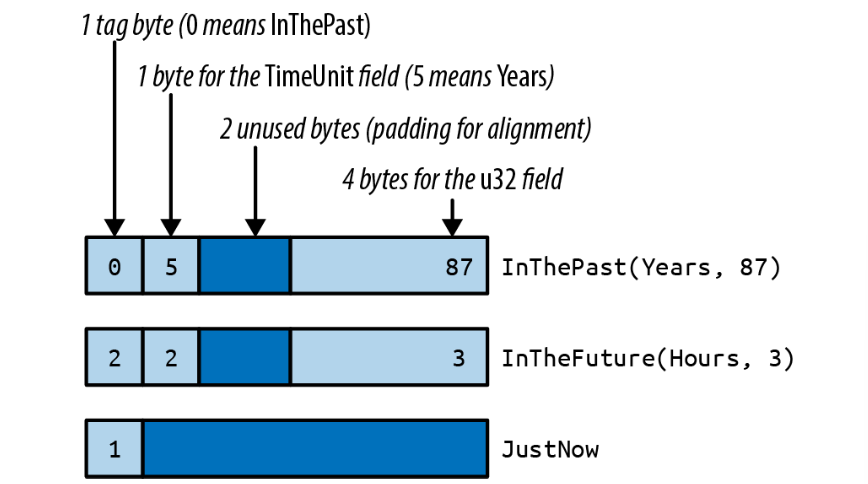
\includegraphics[width=0.9\textwidth]{../img/f10-1.png}
    \caption{内存中的\texttt{RoughTime}值}
    \label{f10-1}
\end{figure}

对于枚举的布局Rust不做任何保证。然而，为了给将来的优化留下余地，在一些情况下它可能会用比图中所示更加高效的方式包装一个枚举。例如，一些泛型结构体可以不用标签存储，我们稍后会讲到它。

\subsection{使用枚举实现富数据结构}

枚举在实现树形结构时也很有用。例如，假设一个Rust程序要处理任意的Json数据。在内存中，任何Json文档都可以被表示为一个这种Rust类型的值：
\begin{minted}{Rust}
    use std::collections::HashMap;

    enum Json {
        Null,
        Boolean(bool),
        Number(f64),
        String(String),
        Array(Vec<Json>),
        Object(Box<HashMap<String, Json>>),
    }
\end{minted}

与Rust代码相比，用英文来解释这个数据结构也不会再有太大的改进了。JSON标准定义了可以出现在JSON文档中的数据类型：\texttt{null}、布尔值、数字、字符串、JSON值的数组、以及带有字符串键和JSON值的对象。这个\texttt{Json}枚举简单地列出了这些类型。

这并不是一个假想的例子。你可以在\texttt{serde\_json} crate中找到一个非常相似的枚举，它是一个用于Rust结构体序列化的库，也是crates.io上下载次数最多的crate之一。

用于表示\texttt{Object}的\texttt{HashMap}外层的\texttt{Box}只是为了让\texttt{Json}值更加紧凑。在内存中，\texttt{Json}类型的值将占据4个机器字。\texttt{String}和\texttt{Vec}都是3个字，Rust会再添加一个字节的标签，再加上对齐所以总共是4个字。\texttt{Null}和\texttt{Boolean}值没有足够的数据利用全部的空间，但所有的\texttt{Json}值大小必须相同，因此这时多余的空间就被浪费了。\hyperref[f10-2]{图10-2}展示了一些示例的\texttt{Json}值在内存中的实际视图。

\begin{figure}[htbp]
    \centering
    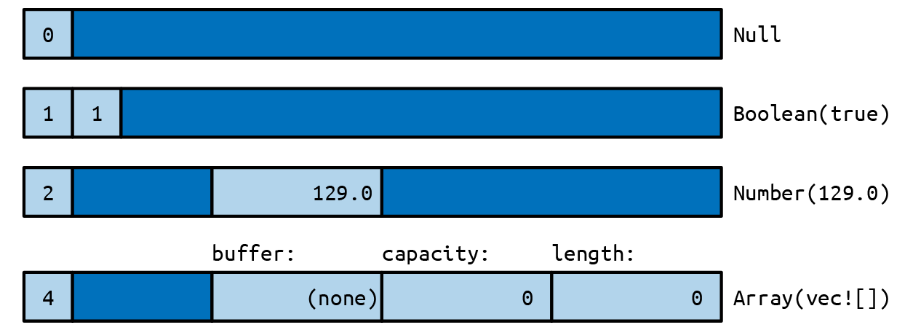
\includegraphics[width=0.8\textwidth]{../img/f10-2.png}
    \caption{内存中的\texttt{Json}值}
    \label{f10-2}
\end{figure}

一个\texttt{HashMap}会更大如果我们一定要在每一个\texttt{Json}值中给它留出空间，它们将会变得更大，也就是8个字。但\texttt{Box<HashMap>}是单个字：它只是一个指向堆上分配的数据的指针。我们甚至可以通过装箱更多的字段来让\texttt{Json}变得更加紧凑。

这里优秀的地方在于，我们如此简单的就完成了这一切。如果是在C++中，可能要写一个这样的一个类才行：
\begin{minted}{Rust}
    class JSON {
    private:
        enum Tag {
            Null, Boolean, Number, String, Array, Object
        };
        union Data {
            bool boolean;
            double number;
            shared_ptr<string> str;
            shared_ptr<vector<JSON>> array;
            shared_ptr<unordered_map<string, JSON>> object;

            Data() {}
            ~Data() {}
            ...
        };
        
        Tag tag;
        Data data;
    
    public:
        bool is_null() const { return tag == Null; }
        bool is_boolean const { return tag == Boolean; }
        bool get_boolean() const {
            assert(is_boolean());
            return data.boolean;
        }
        void set_boolean(bool value) {
            this->~JSON();  // 清除string/array/object值
            tag = Boolean;
            data.boolean = value;
        }
        ...
    };
\end{minted}

30行代码，我们才刚刚开始。这个类还需要构造函数、析构函数、一个赋值运算符。另一种方案是通过继承，首先创建一个基类\texttt{JSON}和它的子类\texttt{JSONBoolean}、\texttt{JSONString}等等。无论哪种方式，等到完成之后，我们的C++ JSON库都要有一堆代码了。其他程序员需要花费不少精力来阅读和使用它。而Rust的整个枚举只需要8行代码。

\subsection{泛型枚举}
枚举可以是泛型的。标准库的两个例子几乎是整个语言中使用最广泛的数据类型：
\begin{minted}{Rust}
    enum Option<T> {
        None,
        Some(T),
    }

    enum Result<T, E> {
        Ok(T),
        Err(E),
    }
\end{minted}

到现在这些类型你应该已经很熟悉了，泛型枚举的语法和泛型结构体完全相同。

一个不明显的细节是当类型\texttt{T}是引用、\texttt{Box}或其他智能指针类型时Rust可以省略\texttt{Option<T>}的标签字段。因为这些指针类型中的任何一个都不允许为0，所以Rust可以用单个机器字来表示\texttt{Option<Box<i32>>}：用0表示\texttt{None}，用非0表示\texttt{Some}指针。这使得这样的\texttt{Option}类型与C和C++中可以为空的指针值非常相似。不同之处在于Rust的类型系统要求你必须先检查\texttt{Option}的值是\texttt{Some}，然后才能使用它内含的值。这有效的避免了空指针解引用。

泛型数据结构体可以用很少的几行代码构建：
\begin{minted}{Rust}
    // 一个`T`类型的有序集合
    enum BinaryTree<T> {
        Empty,
        NonEmpty(Box<TreeNode<T>>),
    }

    // 二叉树的一部分
    struct TreeNode<T> {
        element: T,
        left: BinaryTree<T>,
        right: BinaryTree<T>,
    }
\end{minted}

这几行代码定义了一个可以存储任意数量的\texttt{T}类型值的\texttt{BinaryTree}类型。

这两个定义包含了大量信息，所以我们将花费一些时间把代码翻译为中文。每一个\texttt{BinaryTree}值是\texttt{Empty}或者\texttt{NonEmpty}。如果它是\texttt{Empty}，那么它不包含任何数据。如果是\texttt{NonEmpty}，那么它会包含一个\texttt{Box}，这个指针指向一个在堆上分配的\texttt{TreeNode}值。

每一个\texttt{TreeNode}值包含一个实际的元素，和两个\texttt{BinaryTree}值。这意味着一棵树可以包含子树，因此一个\texttt{NonEmpty}树可以包含任意数量的后台节点。

一个\texttt{BinaryTree<\&str>}类型的值的视图如\hyperref[f10-3]{图10-3}所示。因为对于\texttt{Option<Box<T>>}，Rust会省略标签字段，所以一个\texttt{BinaryTree}值只占一个机器字。

\begin{figure}[htbp]
    \centering
    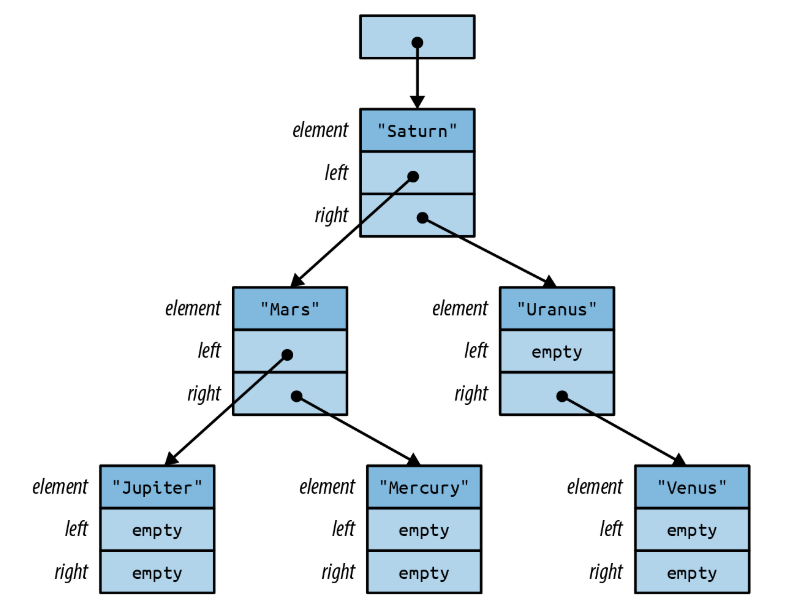
\includegraphics[width=0.9\textwidth]{../img/f10-3.png}
    \caption{一个包含6个字符串的\texttt{BinaryTree}}
    \label{f10-3}
\end{figure}

构建这棵树中的节点非常直观：
\begin{minted}{Rust}
    use self::BinaryTree::*;
    let jupiter_tree = NonEmpty(Box::new(TreeNode {
        element: "Jupiter",
        left: Empty,
        right: Empty,
    }));
\end{minted}

更大的树可以通过较小的树构建：
\begin{minted}{Rust}
    let mars_tree = NonEmpty(BOx::new(TreeNode {
        element: "Mars",
        left: jupiter_tree,
        right: mercury_tree,
    }));
\end{minted}

自然地，这个赋值会把\texttt{jupiter\_node}和\texttt{mercury\_node}的所有权移动到新的父节点里。

树的其他部分遵循相同的模式。根节点和其它节点不同：
\begin{minted}{Rust}
    let tree = NonEmpty(Box::new(TreeNode {
        element: "Saturn",
        left: mars_tree,
        right: uranus_tree,
    }));
\end{minted}

在这一章的后续部分中，我们将介绍怎么在\texttt{BinaryTree}类型上实现一个\texttt{add}方法，这样我们就可以这样写：
\begin{minted}{Rust}
    let mut tree = BinaryTree::Empty;
    for planet in planets {
        tree.add(planet);
    }
\end{minted}

无论你之前用什么语言，在Rust中创建像\texttt{BinaryTree}这样的数据结构都需要一些练习。一开始把\texttt{Box}放在哪可能并不明显。一种寻找设计的方法是画一幅像\hyperref[f10-3]{图10-3}这样的内存布局图。然后根据图设计代码：每一个矩形都是一个结构体或者元组，每一个箭头都是一个\texttt{Box}或者其他智能指针。搞清楚每个字段的类型有点困难，但解决难题的回报是控制程序的内存使用。 

现在就到了我们在本章开始时提到的“代价”。枚举的标签字段要占用很小的内存，最糟的情况下要占用8个字节，但这种情况通常非常少见。枚举真正的缺点（如果它能被称为缺点的话）是Rust不能忽略安全性、不管当前的值是什么直接尝试访问字段：
\begin{minted}{Rust}
    let r = shape.radius;   // 错误：`Shape`类型没有字段`radius`
\end{minted}

访问枚举中的值的唯一方式是：使用枚举，这是一种安全的方式。

\section{模式}

回顾一下我们在本章中定义过的\texttt{RoughTime}：
\begin{minted}{Rust}
    enum RoughTime {
        InThePast(TimeUnit, u32),
        JustNow,
        InTheFuture(TimeUnit, u32),
    }
\end{minted}

假设你有一个\texttt{RoughTime}值并且你想在网页中显示它。你需要访问值里的\texttt{TimeUnit}和\texttt{u32}字段。Rust不允许你直接通过\texttt{rough\_time.0}和\texttt{rough\_time.1}访问它们，因为毕竟此时值也可能是\texttt{RoughTime::JustNow}，而它没有字段。那么，你怎么获取数据呢？

你需要一个\texttt{match}表达式：
\begin{minted}[linenos,numbersep=-1em]{Rust}
    fn rough_time_to_english(rt: RoughTime) -> String {
        match rt {
            RoughTime::InThePast(units, count) =>
                format!("{} {} ago", count, units.plural()),
            RoughTime::JustNow =>
                format!("just now"),
            RoughTime::InTheFuture(units, count) =>
                format!("{} {} from now", count, units.plural()),
        }
    }
\end{minted}
\texttt{match}会进行模式匹配。在这个例子中，\emph{模式}是第3、5、7行中出现在\texttt{=>}符号左边的部分。匹配\texttt{RoughTime}值的模式看起来就像是一个创建\texttt{RoughTime}值的表达式。这并不是巧合。表达式\emph{产生}值，模式\emph{消耗}值。它们使用相同的语法。

让我们逐步看看运行这个\emph{match}表达式时发生了什么。假设\texttt{rt}的值是\texttt{RoughTime::InTheFuture(TimeUnit::Months, 1)}。Rust首先尝试将这个值和第3行的模式匹配。正如\hyperref[f10-4]{图10-4}所示，它并不能匹配。

\begin{figure}[htbp]
    \centering
    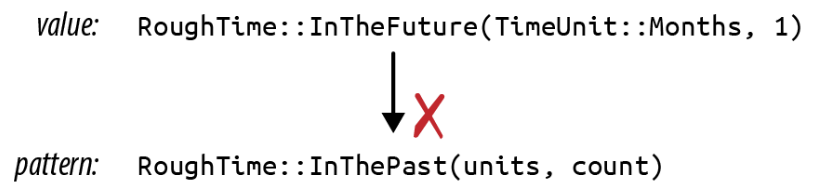
\includegraphics[width=0.8\textwidth]{../img/f10-4.png}
    \caption{一个\texttt{RoughTime}值和不匹配的模式}
    \label{f10-4}
\end{figure}

Rust中用于匹配一个枚举、结构体或者元组的模式的工作原理就好像简单地从左到右扫描，检查模式中的每个部分来看看是不是和值匹配。如果不是，Rust会移动到下一个模式。

第3和第5行的模式都匹配失败。但第7行的模式成功了（\hyperref[f10-5]{图10-5}）。

\begin{figure}[htbp]
    \centering
    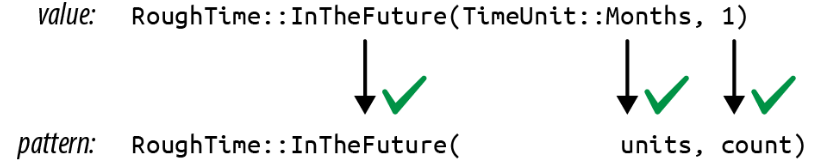
\includegraphics[width=0.8\textwidth]{../img/f10-5.png}
    \caption{一个成功的匹配}
    \label{f10-5}
\end{figure}

当一个模式包含像\texttt{units}和\texttt{count}这样的简单标识符时，在匹配之后的代码中它们会变为局部变量。当前值里的任何内容都会被拷贝或移动到新的变量中。Rust把\texttt{TimeUnit::Months}存储在\texttt{units}中，把\texttt{1}存储在\texttt{count}中，然后运行第8行的代码，最后返回字符串\texttt{"1 months from now"}。

这个输出有一点语法上的错误，可以通过给\texttt{match}添加另一个分支来修正：
\begin{minted}{Rust}
    RoughTime::InTheFuture(unit, 1) =>
        format!("a {} from now", unit.singular()),
\end{minted}

只有当\texttt{count}字段恰好是1时这个分支才能匹配。注意这一段新代码必须添加到第7行之前。如果我们把它添加在最后，那么执行流永远不会到达它，因为第7行匹配所有的\texttt{InTheFuture}值。如果你犯了这种错误，Rust编译器会给出一个“不可达的模式”警告。

即使有了新的代码，\texttt{RoughTime::InTheFuture(TimeUnit::Hours, 1)}仍然有一个问题：结果\texttt{"a hour from now"}在英语中并不是完全正确。这可以通过给\texttt{match}添加另一个分支来修复。

正如这个例子所示，模式匹配和枚举协同工作，甚至可以测试它们包含的值，这使得\texttt{match}表达式成为C的\texttt{switch}语句的一个更强大、更灵活的替代。

到目前为止，我们只见到了匹配枚举值的模式。其实它还有更多用途。Rust的模式有它们自己的语言，\hyperref[t10-1]{表10-1}中进行了总结。我们将用本章中剩下的大部分内容来展示表中的特性。

\begin{table}[htbp]
    \centering
    \caption{模式}
    \label{t10-1}
    \begin{tabular}{p{0.15\textwidth}p{0.35\textwidth}p{0.4\textwidth}}
        \hline
        \textbf{模式类型} & \textbf{示例} & \textbf{注释} \\
        \hline
        字面量  & \makecell[l]{\texttt{100} \\ \texttt{"name"}} & 匹配一个精确值，也可以使用一个\texttt{const}的值的名称    \\
        \rowcolor{tablecolor}
        范围    & \makecell[l]{\texttt{0 ..= 100} \\ \texttt{'a' ..= 'k'}}  & 匹配范围内的任何值，包括终点值 \\
        通配符  & \texttt{\_}   & 匹配任何值并忽略  \\
        \rowcolor{tablecolor}
        变量    & \makecell[l]{\texttt{name} \\ \texttt{mut count}} & 类似\texttt{\_}但是把值移动或拷贝进新的局部变量   \\
        \texttt{ref}变量    & \makecell[l]{\texttt{ref field} \\ \texttt{ref mut field}}    & 借用匹配的值的引用，而不是移动或拷贝它    \\
        \rowcolor{tablecolor}
        带子模式的绑定  & \makecell[l]{\texttt{val @ 0 ..= 99} \\ \texttt{ref circle @ Shape::Circle \{ .. \}}} & 匹配@右侧的模式，使用左侧作为变量名   \\
        枚举模式    & \makecell[l]{\texttt{Some(value)} \\ \texttt{None} \\ \texttt{Pet::Orca}} & \\
        \rowcolor{tablecolor}
        元组模式    & \makecell[l]{\texttt{(key, value)} \\ \texttt{(r, g, b)}} & \\
        数组模式    & \makecell[l]{\texttt{[a, b, c, d, e, f, g]} \\ \texttt{[heading, carom, correction]}} & \\
        \rowcolor{tablecolor}
        切片模式    & \makecell[l]{\texttt{[first, second]} \\ \texttt{[first, \_, third]} \\ \texttt{[first, .., nth]} \\ \texttt{[]}}  & \\
        结构体模式  & \makecell[l]{\texttt{Color(r, g, b)} \\ \texttt{Point \{ x, y \}} \\ \texttt{Card \{ suit: Clubs, rank: n \}} \\ \texttt{Account \{ id, name, .. \}}} & \\
        \rowcolor{tablecolor}
        引用    & \makecell[l]{\texttt{\&value} \\ \texttt{\&(k, v)}}   & 只匹配引用值 \\
        多重模式    & \texttt{'a' | 'A'}    & 只能用作可反驳的模式（\texttt{match, if let, while let}） \\
        \rowcolor{tablecolor}
        守卫表达式  & \texttt{x if x * x <= r2} & 只能在\texttt{match}中使用（在\texttt{let}等表达式中无效） \\
    \end{tabular}
\end{table}

\subsection{模式中的字面量、变量和通配符}
到目前为止，我们已经展示了\texttt{match}表达式和枚举一起使用，其实其它类型也可以用模式来匹配。当你需要类似C的\texttt{switch}语句的功能时，可以使用处理整数值的\texttt{match}表达式。整数字面量例如\texttt{0}和\texttt{1}可以用作模式：
\begin{minted}{Rust}
    match meadow.count_rabbits() {
        0 => {} // 什么都不输出
        1 => println!("A rabbit is nosing around in the clover."),
        n => println!("There are {} rabbits hopping about in the meadow", n),
    }
\end{minted}

当草地上没有兔子时模式\texttt{0}会匹配，当只有一只时\texttt{1}会匹配。如果有两只或者更多兔子，就会到达第三个模式\texttt{n}。这个模式只有一个变量名。它可以匹配任何值，被匹配的值会被移动或拷贝进新的局部变量。因此在这个例子中，\texttt{meadow.count\_rabbits()}的值被存储在一个新的局部变量\texttt{n}中，然后我们打印出它。

其他的字面量也可以用作模式，包括布尔值、字符、甚至字符串：
\begin{minted}{Rust}
    let calendar = match settings.get_string("calendar") {
        "gregorian" =>  Calendar::Gregorian,
        "chinese" => Calendar::Chinese,
        "ethiopian" => Calendar::Ethiopian,
        other => return parse_error("calendar", other),
    };
\end{minted}

在这个例子中，\texttt{other}和上个例子中的\texttt{n}一样用作匹配任何值的模式。这些模式和\texttt{switch}语句中的\texttt{default}标签一样，用来匹配其他所有模式都匹配不了的值。

如果你需要一个匹配所有值的模式，但又不关心匹配到的值，你可以使用单个下划线\texttt{\_}作为模式，也就是\emph{通配模式}：
\begin{minted}{Rust}
    let caption = match photo.tagged_pet() {
        Pet::Tyrannosaur => "RRRAAAAAHHHHHH",
        Pet::Samoyed => "*dog thoughts*",
        _ => "I'm cute, love me",   // 通用标题，用于任何宠物
    };
\end{minted}

通配模式匹配任何值，但并不存储它。因为Rust要求每一个\texttt{match}表达式要能处理所有可能的值，因此最后通常需要一个通配符。即使你非常确信其他的情况不会发生，你也必须至少添加一个fallback分支，这个分支里可以直接panic：
\begin{minted}{Rust}
    // 有很多形状，但我们只支持“选择”文本或者一个矩形区域。
    // 你不能选择一个椭圆或者梯形。
    match document.selection() {
        Shape::TextSpan(start, end) => paint_text_selection(start, end),
        Shape::Rectangle(rect) => paint_rect_selection(rect),
        _ => panic!("unexpected selection type"),
    }
\end{minted}

\subsection{元组和结构体模式}
元组模式匹配元组。当你想在单个\texttt{match}中获得数据的多个部分时它们会很有用：
\begin{minted}{Rust}
    fn describe_point(x: i32, y: i32) -> &'static str {
        use std::cmp::Ordering::*;
        match (x.cmp(&0), y.cmp(&0)) {
            (Equal, Equal) => "at the origin",
            (_, Equal) => "on the x axis",
            (Equal, _) => "on the y axis",
            (Greater, Greater) => "in the first quadrant",
            (Less, Greater) => "in the second quadrant",
            _ => "somewhere else",
        }
    }
\end{minted}

结构体模式要使用花括号，就和结构体表达式一样。它们可以包含每个字段的子模式：
\begin{minted}{Rust}
    match balloon.location {
        Point { x: 0, y: height } =>
            println!("straight up {} meters", height),
        Point { x: x, y: y } =>
            println!("at ({}m, {}m)", x, y),
    }
\end{minted}

在这个例子中，如果第一个分支匹配了，那么\texttt{balloon.location.y}会被存储到新的局部变量\texttt{height}。

假设\texttt{balloon.location}是\texttt{Point \{ x: 30, y: 40 \}}。和之前一样，Rust会按照\hyperref[f10-6]{图10-6}的顺序检查每一个模式的每一个部分。

\begin{figure}[htbp]
    \centering
    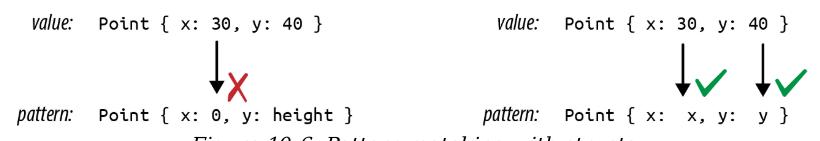
\includegraphics[width=0.8\textwidth]{../img/f10-6.png}
    \caption{结构体模式匹配}
    \label{f10-6}
\end{figure}

第二个分支可以匹配，因此输出将是\texttt{at (30m, 40m)}。

当匹配结构体时类似\texttt{Point \{ x: x, y: y \}}的模式非常常见，多余的名字也只会扰乱视觉，因此Rust为此支持一种缩写形式\texttt{Point \{x, y\}}。含义和之前相同，这个模式也会把点的\texttt{x}字段存储在新的局部变量\texttt{x}、把\texttt{y}字段存储在新的局部变量\texttt{y}。

即使有了缩写形式，如果我们要匹配一个很大的结构体但又只关心少数字段时还是会很麻烦：
\begin{minted}{Rust}
    match get_account(id) {
        ...
        Some(Account {
                name, language, // 我们关心的两个字段
                id: _, status: _, address: _, birthday: _, eye_color: _,
                pet: _, security_question: _, hashed_innermost_secret: _,
                is_adamantium_preferred_customer: _, }) =>
            language.show_custom_greeting(name),
    }
\end{minted}

为了避免这种情况，可以使用\texttt{..}告诉Rust你不关心其他的字段：
\begin{minted}{Rust}
    Some(Account { name, language, .. }) =>
        language.show_custom_greeting(name),
\end{minted}

\subsection{数字和切片模式}
数组模式匹配数组。它们被通常被用来过滤出某些特殊值，当数组的不同位置的含义不同时它们也会变得很有用。

例如，当把色相、饱和度、亮度(HSL)颜色值转换为红绿蓝(RGB)颜色值时，亮度为0的颜色就是黑、而亮度为满的颜色就是白。我们可以使用\texttt{match}表达式来简单地处理这些情况：
\begin{minted}{Rust}
    fn hsl_to_rgb(hsl: [u8; 3]) -> [u8; 3] {
        match hsl {
            [_, _, 0] => [0, 0, 0],
            [_, _, 255] => [255, 255, 255],
            ...
        }
    }
\end{minted}

切片模式与此类似，单核数组不同的是，切片的长度可以变化。因此切片模式并不只匹配值，还要匹配长度。切片模式中的\texttt{..}匹配任意数量的元素：
\begin{minted}{Rust}
    fn greet_people(names: &[&str]) {
        match names {
            [] => { println!("Hello, nobody.") },
            [a] => { println!("Hello, {}.", a) },
            [a, b] => { println!("Hello, {} and {}.", a, b) },
            [a, .., b] => { println!("Hello, everyone from {} to {}.", a, b) }
        }
    }
\end{minted}

\subsection{引用模式}
Rust模式支持两种和引用有关的特性。\texttt{ref}模式会借用被匹配的值，\texttt{\&}模式匹配引用。我们将首先介绍\texttt{ref}模式。

匹配一个非拷贝类型的值会移动这个值。继续上面的例子，下面的代码是无效的：
\begin{minted}{Rust}
    match account {
        Account { name, language, .. } => {
            ui.greet(&name, &language);
            ui.show_settings(&account); // error: borrow of moved value: `account`
        }
    }
\end{minted}

这里，字段\texttt{account.name}和\texttt{account.language}被移动进局部变量\texttt{name}和\texttt{language}中。\texttt{account}的其他部分被丢弃。这就是为什么我们不能再借用它的引用。

如果\texttt{name}和\texttt{language}都是可拷贝的值，Rust将会拷贝字段而不是移动它们，代码将没有问题。但假设它们就是\texttt{String}，那我们该怎么办？

我们需要一种模式\emph{借用}被匹配的值而不是移动它们。\texttt{ref}关键字就是为此而生：
\begin{minted}{Rust}
    match account {
        Account { ref name, ref language, .. } => {
            ui.greet(name, language);
            ui.show_settings(&account); // ok
        }
    }
\end{minted}

现在局部变量\texttt{name}和\texttt{language}都是\texttt{account}中相应字段的引用。因此\texttt{account}只是被借用，并没有被消耗，所以继续用它调用方法也是OK的。

你可以使用\texttt{ref mut}来借用\texttt{mut}引用：
\begin{minted}{Rust}
    match line_result {
        Err(ref err) => log_error(err), // `err`是&Error(shared ref)
        Ok(ref mut line) => {           // `line`是&mut String(mut ref)
            trim_comments(line);        // 修改String
            handle(line);
        }
    }
\end{minted}

模式\texttt{Ok(ref mut line)}匹配任何成功值，并借用存储在里面的成功值的\texttt{mut}引用。

另一种相反的引用模式是\texttt{\&}模式。一个以\texttt{\&}开始的模式只能匹配引用：
\begin{minted}{Rust}
    match sphere.center() {
        &Point3d { x, y, z } => ...
    }
\end{minted}

在这个例子中，假设\texttt{sphere.center()}返回一个\texttt{sphere}的私有字段的引用，这在Rust中是很常见的。返回的值是一个\texttt{Point3d}的引用。如果中心在原点的话，\texttt{sphere.center()}会返回\texttt{\&Point3d \{ x: 0.0, y: 0.0, z: 0.0 \}}。

模式匹配按照\hyperref[f10-7]{图10-7}进行。

\begin{figure}[htbp]
    \centering
    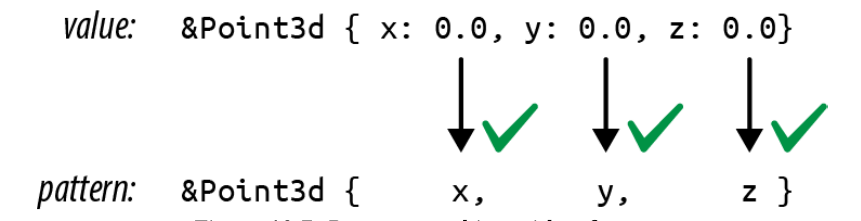
\includegraphics[width=0.8\textwidth]{../img/f10-7.png}
    \caption{引用的模式匹配}
    \label{f10-7}
\end{figure}

这里有一点诡异，因为Rust在这里解除了引用，也就是\texttt{*}运算符的功能。要住的是模式和表达式天然是相反的。表达式\texttt{(x, y)}把两个值放入一个新的元组中，而模式\texttt((x, y))恰好相反：它匹配一个元组然后取出两个值。\texttt{\&}也是一样，在表达式里，\texttt{\&}创建一个引用；在模式里，\texttt{\&}匹配一个引用。

匹配一个引用遵循我们期望的所有规则。生命周期是强制的。你不能通过共享引用获取\texttt{mut}访问权限。你不能将值移动出引用，即使是\texttt{mut}引用。当我们匹配\texttt{\&Point3d \{ x, y, z \}}时，变量\texttt{x, y, z}都是坐标的拷贝，原本的\texttt{Point3d}值还是完整的。只有当这些字段都是拷贝类型才可以正常工作。如果我们想对结构体中一个不可拷贝的字段这么做，我们会遇到错误：
\begin{minted}{Rust}
    match friend.borrow_car() {
        Some(&Car { engine, .. }) => // error: can't move out of borrow
            ...
        None => {}
    }
\end{minted}

把一辆借来的车报废是不好的，Rust也不会允许这么做。你可以使用\texttt{ref}模式来借用一个引用，这样就不用拥有它：
\begin{minted}{Rust}
    Some(&Car { ref engine, .. }) => // ok, engine is a reference
\end{minted}

再来看另一个\texttt{\&}模式的例子。假设我们有一个迭代器\texttt{chars}迭代一个字符串里的所有字符，并且它有一个方法\texttt{chars.peek()}返回一个\texttt{Option<\&char>}：一个指向下一个字符的引用，如果有的话。（这类迭代器确实返回一个\texttt{Option<\&ItemType>}，我们将在\hyperref[ch15]{第15章}中见到。）

一个程序可以使用\texttt{\&}来获得指向的字符：
\begin{minted}{Rust}
    match chars.peek() {
        Some(&c) => println!("coming up: {:?}", c),
        None => println!("end of chars"),
    }
\end{minted}

\subsection{匹配守卫}
有时一个匹配分支还有附加的条件必须要满足。假设我们在实现一个六边形空间内的棋子游戏，玩家只需要点击即可移动棋子。为了确认点击时有效的，我们可能要尝试类似这样的代码：
\begin{minted}{Rust}
    fn check_move(current_hex: Hex, click: Point) -> game::Result<Hex> {
        match point_to_hex(click) {
            None =>
                Err("That's not a game space."),
            Some(current_hex) => // 尝试匹配用户是不是点击了当前位置
                                 // (这样是错误的：原因如下)
                Err("You are already there! You must click somewhere else."),
            Some(other_hex) =>
                Ok(other_hex)
        }
    }
\end{minted}

这样是错误的，因为模式里的标识符会引入\emph{新的}变量。模式\texttt{Some(current\_hex)}会创建一个新的叫\texttt{current\_hex}的局部变量，然后遮蔽参数\texttt{current\_hex}。Rust会为这段代码报出好几个警告——尤其是，最后一个\texttt{match}分支不可达。一种修复这个问题的方法是简单地在分支中使用一个\texttt{if}表达式：
\begin{minted}{Rust}
    match point_to_hex(click) {
        None => Err("That's not a game space."),
        Some(hex) => {
            if hex == current_hex {
                Err("You are already there! You must click somewhere else")
            } else {
                Ok(hex)
            }
        }
    }
\end{minted}

不过Rust还提供了\emph{匹配守卫(match guard)}：模式和分支的\texttt{=>}词元中间的\texttt{if CONDITION}条件必须满足才能匹配：
\begin{minted}{Rust}
    match point_to_hex(click) {
        None => Err("That's not a game space."),
        Some(hex) if hex == current_hex =>
            Err("You are already there! You must click somewhere else"),
        Some(hex) => Ok(hex)
    }
\end{minted}

如果模式匹配，但条件不满足，那么将会继续匹配下一个分支。

\subsection{匹配多种可能}
竖线(|)可以用于在一个\texttt{match}分支中组合多个模式：
\begin{minted}{Rust}
    let at_end = match chars.peek() {
        Some(&'\r') | Some(&'\n') | None => true,
        _ => false,
    };
\end{minted}

在一个表达式中，|是位或运算符，但这里它的功能就像是普通表达式中的\texttt{||}。如果\texttt{chars.peek()}能匹配三个模式中的任意一个，\texttt{at\_end}就会被设为\texttt{true}。

使用\texttt{..=}来匹配范围内的值。范围模式包括起点和终点值，因此\texttt{'0' ..= '9'}匹配所有的ASCII数字：
\begin{minted}{Rust}
    match next_char {
        '0'..='9' => self.read_number(),
        'a'..='z' | 'A'..='Z' => self.read_word(),
        ' ' | '\t' | '\n' => self.skip_whitespace(),
        _ => self.handle_punctuation(),
    }
\end{minted}

Rust（目前）不允许在模式中使用尾开区间例如\texttt{0..100}。

\subsection{绑定和\texttt{@}模式}




\chapter{trait与泛型}\label{ch11}

\emph{[A] computer scientist tends to be able to deal with nonuniform structures—case 1, case 2, case 3—while a mathematician will tend to want one unifying axiom that governs an entire system.}

\begin{flushright}
    ——Donald Knuth
\end{flushright}

编程界中最伟大的发现之一就是可以编写处理多种不同类型的代码，\emph{即使是还没有定义出来的类型也可以}。这里有两个例子：
\begin{itemize}
    \item \texttt{Vec<T>}是泛型的：你可以创建一个任意类型的vector，包括你自己定义的类型，即使\texttt{Vec}的作者完全不知道这个类型。
    \item 很多类型都有\texttt{.write()}方法，包括\texttt{File}和\texttt{TcpStream}。你的代码可以通过引用获取一个writer(任意的writer)，并向它写入数据。你的代码不需要关心那个writer到底是什么类型。然后，如果有人添加了一个新的writer类型，你的代码将会自动支持它。
\end{itemize}

当然，这并不是什么新鲜的功能。它被称为\emph{多态(polymorphism)}，是20世纪70年代很热门的新的编程语言技术。但现在它已经非常普遍了。Rust使用两个相关的特性来支持多态：trait和泛型。很多程序员可能已经很熟悉这两个概念了，但Rust采用了一种受Haskell的typeclass启发的新方法。

\emph{trait}是Rust中的接口或抽象基类。首先，它们看起来很像Java或C\#中的接口。用于写入字节的trait叫做\texttt{std::io::Write}，它在标准库中的定义看起来像这样：
\begin{minted}{Rust}
    trait Write {
        fn write(&mut self, buf: &[u8]) -> Result<usize>;
        fn flush(&mut self) -> Result<()>;

        fn write_all(&mut self, buf: &[u8]) -> Result<()> { ... }
        ...
    }
\end{minted}

这个trait提供了几个方法，我们只展示了前三个。

标准类型\texttt{File}和\texttt{TcpStream}都实现了\texttt{std::io::Write}。\texttt{Vec<u8>}也是。这三个类型都提供\texttt{.write()}、\texttt{.flush()}等方法。使用writer的代码不需要关心它的类型，像这样：
\begin{minted}{Rust}
    use std::io::Write;

    fn say_hello(out: &mut dyn Write) -> std::io::Result<()> {
        out.write_all(b"hello world\n")?;
        out.flush()
    }
\end{minted}

\texttt{out}的类型是\texttt{\&mut dyn Write}，意思是“任何实现了。\texttt{Write} trait的值的可变引用”。我们可以把任何这样的值的可变引用传递给\texttt{say\_hello}：
\begin{minted}{Rust}
    use std::fs::File;
    let mut local_file = File::create("hello.txt")?;
    say_hello(&mut local_file)?;    // 可以工作

    let mut bytes = vec![];
    say_hello(&mut bytes)?;         // 也可以工作
    assert_eq!(bytes, b"hello world\n");
\end{minted}

这一章首先展示trait怎么使用、怎么工作、怎么定义自己的trait。但trait的用途比我们目前提到的更多。我们将使用它们给现有类型添加扩展的方法，甚至像\texttt{str}和\texttt{bool}这种内建类型也可以。我们将会解释为什么给一个类型添加trait不会消耗多余的内存，以及如何在没有虚方法开销的情况下使用trait。我们将看到一些Rust提供的用于操作符重载和其他特性的语言内建的trait。我们还将介绍\texttt{Self}类型、关联函数、关联类型。Rust从Haskell中提取了这三个特性，它们可以优雅地解决其他语言中需要通过变通的方法或者hack才能解决的问题。 

\emph{泛型}是Rust中另一种形式的多态。类似于C++的模板，一个泛型函数或类型可以用于多种不同的类型：
\begin{minted}{Rust}
    /// 给定两个值，找出较小的那个
    fn min<T: Ord>(value1: T, value2: T) -> T {
        if value1 <= value2 {
            value1
        } else {
            value2
        }
    }
\end{minted}

这个函数中的\texttt{<T: Ord>}意味着\texttt{min}可以用于任何实现了\texttt{Ord} trait的类型\texttt{T}——也就是，任何有序的类型。这样的一个要求被称为\emph{约束(bound)}，因为它列举出了类型\texttt{T}需要满足的限制。编译器会为你实际使用的每一个类型\texttt{T}生成自定义的机器代码。

泛型和trait紧密相关：泛型函数在约束中使用trait来表明它可以用于哪些类型的参数。所以我们还会讨论\texttt{\&mut dyn Write}和\texttt{<T: Write>}有哪些相似和不同之处，以及如何在这种两种使用trait的方式中选择。

\section{使用trait}

一个trait就是一个给定的类型可能支持也可能不支持的特性。通常，一个trait代表一种能力：一个类型可以做的事情。
\begin{itemize}
    \item 一个实现了\texttt{std::io::Write}的值可以写入字节。
    \item 一个实现了\texttt{std::iter::Iterator}的值可以产生值的序列。
    \item 一个实现了\texttt{std::clone::Clone}的值可以产生自身在内存中的克隆。
    \item 一个实现了\texttt{std::fmt::Debug}可以使用\texttt{println!()}的\texttt{\{:?\}}格式说明符进行打印。
\end{itemize}

那4个trait都是Rust标准库的一部分，有很多标准类型都实现了它们。例如：
\begin{itemize}
    \item \texttt{std::fs::File}实现了\texttt{Write} trait，它把字节写入到本地文件。\texttt{std::net::TcpStream}写入到网络连接。\texttt{Vec<u8>}也实现了\texttt{Write}。在字节vector上调用\texttt{.write()}会往尾部添加数据。
    \item \texttt{Range<i32>}(\texttt{0..10}的类型)实现了\texttt{Iterator} trait，一些和切片、哈希表等相关联的迭代器类型也实现了这个trait。
    \item 大多数标准库类型实现了\texttt{Clone}。一些例外主要是像\texttt{TcpStream}这样的不仅仅表示内存中的数据的类型。
    \item 大多数标准库类型支持\texttt{Debug}。
\end{itemize}

有关trait方法有一个不寻常的规则：trait自身必须在作用域里。否则，所有它的方法都会被隐藏：
\begin{minted}{Rust}
    let mut buf: Vec<u8> = vec![];
    buf.write_all(b"hello")?;   // 错误：没有叫`write_all`的方法
\end{minted}

这种情况下，编译器会打印出友好的错误消息建议你添加\texttt{std::io::Write}，然后确实能修复这个问题：
\begin{minted}{Rust}
    use std::io::Write;

    let mut buf: Vec<u8> = vec![];
    buf.write_all(b"hello")?;   // ok
\end{minted}

Rust会有这个规则是因为，正如我们稍后会在本章中看到的，你可以使用trait来给任意类型添加新的方法——即使是标准库的类型例如\texttt{u32}和\texttt{str}。第三方的crate也可以做同样的事情。显然，这会导致名称冲突！但因为Rust让你自己导入你需要使用的trait，所以crate可以轻松地利用这种强大的功能。要想导致冲突，你需要导入两个trait，这两个trait要给同一个类型添加相同名称的方法。这在实践中是很少见的。（如果你确实陷入了冲突中，你可以使用本章稍后会介绍的\nameref{fullymethod}来指明你想要使用哪一个。）

\texttt{Clone}和\texttt{Iterator}的方法不需要特殊的导入是因为它们默认总是在作用域里，它们是标准prelude的一部分：Rust会自动导入每个模块中的名称。事实上，prelude就是一个精心挑选的trait的集合。我们将在\hyperref[ch13]{第13章}中介绍更多有关它们的内容。

C++和C\#程序员可能已经注意到了trait方法很像虚方法。然而，类似上面的函数调用速度很快，与任何其他方法调用一样快。简单来说，这里面并没有多态性。显然\texttt{buf}是一个vector，不是一个文件或者网络连接，所以编译器可以简单地生成一个\texttt{Vec<u8>::write()}的调用。它甚至可以内联这个方法。（C++和C\#通常也会这样，尽管子类化的可能性有时会排除这一点。）只有通过\texttt{\&mut dyn Write}的调用才会有动态分发的开销，这种调用也被称为虚方法调用，类型里的\texttt{dyn}关键字暗示了这一点。\texttt{dyn Write}被称为\emph{trait对象(trait object)}；我们将会在接下来的小节中看到trait对象的技术细节，以及它们与泛型函数的比较。

\subsection{trait对象}\label{traitobject}
在Rust中有两种使用trait来编写多态代码的方式：trait对象和泛型。我们将会首先介绍trait对象，在下一节中介绍泛型。

Rust不允许\texttt{dyn Write}类型的变量：
\begin{minted}{Rust}
    use std::io::Write;

    let mut buf: Vec<u8> = vec![];
    let writer: dyn Write = buf; // 错误：`Write`并没有固定的大小
\end{minted}

一个变量的大小必须在编译期时已知，然而实现了\texttt{Write}的类型可以是任何大小。

如果你来自C\#或者Java的话可能会感觉很惊讶，但原因其实很简单。在Java中，一个\texttt{OutputStream}（Java中类似\texttt{std::io::Write}的标准接口）类型的变量是一个任何实现了\texttt{OutputStream}的对象的引用。它是一个引用的事实不言而喻，C\#以及其他大多数语言中的接口也是一样。

我们在Rust中想要的也是一样的，但是在Rust中引用是显式的：
\begin{minted}{Rust}
    let mut buf: Vec<u8> = vec![];
    let writer: &mut dyn Write = &mut buf;  // ok
\end{minted}

一个trait类型的引用，例如\texttt{writer}，被称为一个\emph{trait对象}。和其他引用一样，一个trait对象指向某个值、它有生命周期、它可以是可变的或者是共享的。

让一个trait对象与众不同的是Rust在编译期通常不知道被引用值的类型是什么。因此一个trait对象包括一点额外的有关被引用值的类型信息。类型信息被严格限制为只有Rust自己可以在幕后使用：当你调用\texttt{writer.write(data)}时，Rust需要这个类型信息来依据\texttt{*writer}的类型动态调用正确的\texttt{write}方法。你不能直接查询类型信息，Rust也不支持将trait对象\texttt{\&mut dyn Write}向下转换回精确的类型例如\texttt{Vec<u8>}。

\subsubsection{trait对象的布局}
在内存中，一个trait对象是一个胖指针，由指向值的指针加上一个指向表示该值类型的表的指针组成。因此每一个trait对象要占两个机器字，如\hyperref[f11-1]{图11-1}所示。

\begin{figure}[htbp]
    \centering
    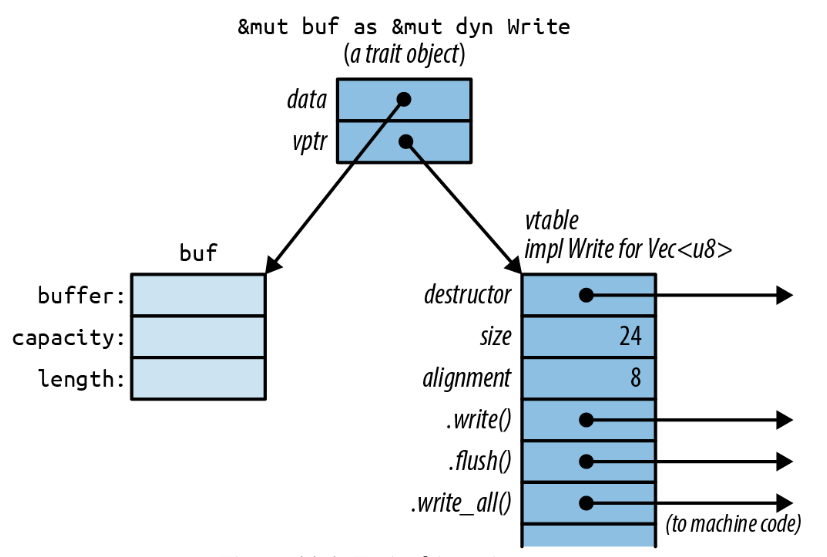
\includegraphics[width=0.9\textwidth]{../img/f11-1.png}
    \caption{内存中的trait对象}
    \label{f11-1}
\end{figure}

C++也有这种运行时的类型信息。它被称为\emph{虚表}或者\emph{vtable}。在Rust中和在C++中一样，vtable只会在编译期生成一次，然后被所有相同类型的对象共享。\hyperref[f11-1]{图11-1}中较深颜色的阴影显示的内容，包括vtable，都是Rust的私有实现。这些字段和数据结构你不能直接访问。当你调用trait对象的方法时语言本身会自动使用vtable来决定要调用哪个实现。

熟练的C++程序员可能会注意到Rust和C++采取的内存策略有些不同。在C++中，虚表指针或者称为\emph{vptr}被存储为结构体的一部分，而Rust使用胖指针来代替。结构体本身不包含任何自身字段之外的东西。这样，一个结构体可以实现一大堆trait而不需要包含一大堆vptr。即使像\texttt{i32}这样的大小还不足以容纳一个vptr的类型，也可以实现trait。

当需要时Rust会自动把普通引用转换为trait对象。这就是为什么我们能在这个例子中直接把\texttt{\&mut local\_file}传递给\texttt{say\_hello}：
\begin{minted}{Rust}
    let mut local_file = File::create("hello.txt")?;
    say_hello(&mut local_file)?;
\end{minted}

\texttt{\&mut local\_file}的类型是\texttt{\&mut File}，而\texttt{say\_hello}的参数类型是\texttt{\&mut dyn Write}。因为\texttt{File}是一种writer，所以Rust允许这种普通引用到trait对象的转换。

同样的，Rust也乐于把\texttt{Box<File>}转换成\texttt{Box<dyn Write>}，它拥有一个在堆上的writer：
\begin{minted}{Rust}
    let w: Box<dyn Write> = Box::new(local_file);
\end{minted}

\texttt{Box<dyn Write>}类似于\texttt{\&mut dyn Write}，是一个胖指针：它包含writer自身的地址和vtable的地址。其他指针类型例如\texttt{Rc<dyn Write>}也一样。

这种转换是唯一创建trait对象的方法。编译器做的工作其实很简单，当转换发生时，Rust知道被引用值的真正类型（这个例子中是\texttt{File}），因此它只是加上了正确的vtable的地址、把普通指针变成了胖指针。

\subsection{泛型函数和类型参数}
在这一章的开始处，我们展示了\texttt{say\_hello()}函数，它以trait对象为参数。让我们把这个函数重新为泛型函数：
\begin{minted}{Rust}
    fn say_hello<W: Write>(out: &mut W) -> std::i9o::Result<()> {
        out.write_all(b"hello world\n")?;
        out.flush()
    }
\end{minted}

只有类型签名改变了：
\begin{minted}{Rust}
    fn say_hello(out: &mut dyn Write)   // 普通函数

    fn say_hello<W: Write>(out: &mut W) // 泛型函数
\end{minted}

让函数变为泛型函数的正是\texttt{<W: Write>}短语，它是一个\emph{类型参数}。它意味着在整个函数体内，\texttt{W}代表任何实现了\texttt{Write} trait的类型。按照习惯，类型参数通常是大写字母。

类型\texttt{W}到底是什么取决于泛型函数如何被调用：
\begin{minted}{Rust}
    say_hello(&mut local_file)?;    // 调用say_hello::<File>
    say_hello(&mut bytes)?;         // 调用say_hello<Vec<u8>>
\end{minted}

当你把\texttt{\&mut local\_file}传递给泛型的\texttt{say\_hello()}函数时，你实际是在调用\texttt{say\_hello::<File>()}。Rust会为这个函数生成机器码，机器码里还会调用\texttt{File::write\_all()}和\texttt{File::flush()}。当你传递\texttt{\&mut bytes}时，你实际是在调用\texttt{say\_hello::<Vec<u8>>()}。Rust会为这个版本的函数生成单独的机器码，然后调用相应的\texttt{Vec<u8>}的方法。在这两种情况下，Rust都从参数的类型推导出类型\texttt{W}，这个过程被称为\emph{单态化(monomorphization)}，编译器会自动进行处理。

你也可以指明类型参数：
\begin{minted}{Rust}
    say_hello::<File>(&mut local_file)?;
\end{minted}

很少情况下才需要显式写出参数，因为Rust通常可以通过参数推断出类型参数。这里，\texttt{say\_hello}泛型函数期望一个\texttt{\&mut W}参数，而我们传入了一个\texttt{\&mut File}，因此Rust推断出\texttt{W = File}。

如果你正在调用的泛型函数并没有足以推断出参数的线索，你需要显式地指明：
\begin{minted}{Rust}
    // 调用一个没有参数的泛型方法collect<C>()
    let v1 = (0 .. 1000).collect();     // 错误：不能推断出类型
    let v2 = (0 .. 1000).collect::<Vec<i32>>(); // ok
\end{minted}

有时我们需要一个类型参数可以支持多种功能。例如，如果我们想打印出一个vector中出现次数最多的10个值，我们需要这些值可以打印：
\begin{minted}{Rust}
    use std::fmt::Debug;

    fn top_ten<T: Debug>(values: &Vec<T>) { ... }
\end{minted}

但这还不够。我们怎么判断哪个值是出现次数最多的？通常的办法是把每个值当作键存入一个哈希表。这意味着这些值需要支持\texttt{Hash}和\texttt{Eq}操作。\texttt{T}的约束还必须包括\texttt{Debug}。这种情况下应该使用的语法是\texttt{+}号：
\begin{minted}{Rust}
    use std::hash::Hash;
    use std::fmt::Debug;

    fn top_ten<T: Debug + Hash + Eq>(values: &Vec<T>) { ... }
\end{minted}

一些类型实现了\texttt{Debug}、一些实现了\texttt{Hash}、一些支持\texttt{Eq}，还有少数类型例如\texttt{u32}和\texttt{String}，实现了这三个trait，如\hyperref[f11-2]{图11-2}所示。

\begin{figure}[htbp]
    \centering
    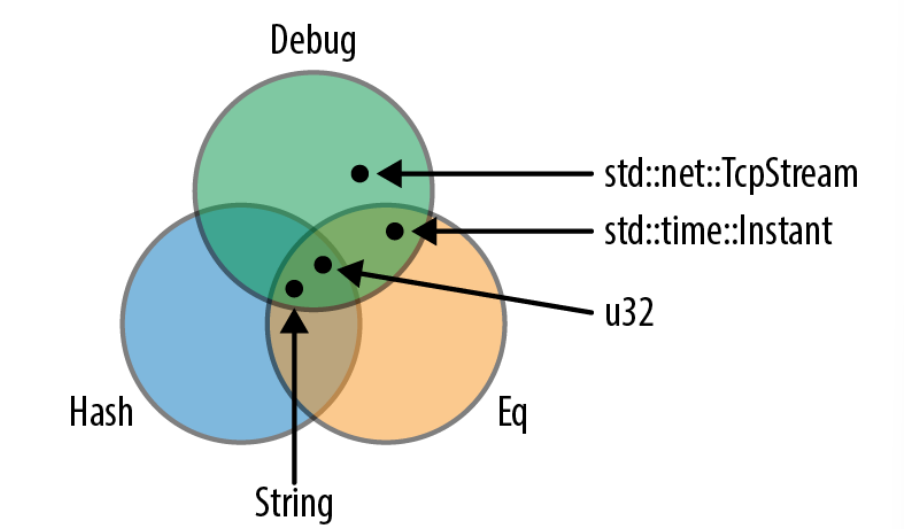
\includegraphics[width=0.8\textwidth]{../img/f11-2.png}
    \caption{trait作为类型的集合}
    \label{f11-2}
\end{figure}

也可以不给类型参数指定任何约束，但这样的话你几乎不能对它进行任何操作。你只能移动它、将它放在box或vector里。

泛型函数可以有多个类型参数：
\begin{minted}{Rust}
    /// 在一个大规模的分区数据集上进行查询。
    /// 见<http://research.google.com/archive/mapreduce.html>。
    fn run_query<M: Mapper + Serialize, R: Reducer + Serialize>(
        data: &DataSet, map: M, reduce: R) -> Results
    { ... }
\end{minted}

正如这个例子展示的一样，约束可能太长以至于很难阅读。Rust提供了使用关键字\texttt{where}的替代语法：
\begin{minted}{Rust}
    fn run_query<M, R>(data: &DataSet, map: M, reduce: R) -> Results
        where M: Mapper + Serialize,
              R: Reducer + Serialize
    { ... }
\end{minted}

类型参数\texttt{M}和\texttt{R}仍然在前边声明，但约束被移动到单独的行。这种\texttt{where}语法可以用于泛型结构体、泛型枚举、类型别名以及方法——任何允许约束的地方。

当然，\texttt{where}语法的一个替代是保持简单：寻找一种不需要大量使用泛型的方法来编写程序。

“\nameref{RefAsArg}”介绍了生命周期的语法。一个泛型函数可以同时有生命周期参数和类型参数。生命周期参数在前：
\begin{minted}{Rust}
    /// 返回`candidates`中距离`target`最近的点的引用。
    fn nearest<'t, 'c, P>(target: &'t P, candidates: &'c [P]) -> &'c P
        where P: MeasureDistance
    {
        ...
    }
\end{minted}

这个函数有两个参数：\texttt{target}和\texttt{candidates}。它们都是引用，但我们给了它们不同的生命周期\texttt{'t}和\texttt{'c}（正如在“\nameref{DistLife}”中讨论的那样）。这个函数可以用于任何实现了\texttt{MeasureDistance} trait的类型\texttt{P}，因此我们可以在一个程序中用\texttt{Point2d}值调用它，而在另一个程序中用\texttt{Point3d}值调用它。

生命周期绝不会影响到机器码。两个\texttt{P}的类型相同但生命周期不同的\texttt{nearest()}的调用，将会调用同一个编译好的函数。只有不同的类型才会导致Rust编译一个泛型函数的多个拷贝。

当然，函数并不是Rust中唯一的泛型代码：
\begin{itemize}
    \item 我们已经在“\nameref{GenStruct}”和“\nameref{GenEnum}”中介绍过泛型类型了。
    \item 一个单独的方法也可以是泛型的，就算定义它的类型不是泛型的：
    \begin{minted}{Rust}
    impl PancakeStack {
        fn push<T: Topping>(&mut self, goop: T) -> PancakeResult<()> {
            goop.pour(&self);
            self.absorb_topping(goop)
        }
    }
    \end{minted}
    \item 类型别名也可以是泛型的：
    \begin{minted}{Rust}
    type PancakeResult<T> = Result<T, PancakeError>;
    \end{minted}
    \item 我们将在本章稍后介绍泛型trait。
\end{itemize}

所有这一节中介绍的特性——约束、\texttt{where}子句、生命周期参数等——可以被用于所有泛型item，而不仅仅是函数。

\subsection{选择哪一种}

\section{完全限定方法调用}\label{fullymethod}


\chapter{运算符重载}\label{ch12}

在\hyperref[ch02]{第2章}的曼德勃罗集绘制器中，我们使用了\texttt{num} crate的\texttt{Complex}类型来表示一个复平面中的点：
\begin{minted}{Rust}
    #[derive(Clone, Copy, Debug)]
    struct Complex<T> {
        /// 复数的实部
        re: T,

        /// 复数的虚部
        im: T,
    }
\end{minted}

我们可以使用Rust的\texttt{+}和\texttt{*}运算符，像操作内建类型一样把\texttt{Complex}值相加和相乘：
\begin{minted}{Rust}
    z = z * z + c;
\end{minted}

你也可以让你自己的类型支持算数和其他运算符，只需要实现一些内建的trait。这被称为\emph{运算符重载(operator overloading)}，它的效果也类似于C++、C\#、Python和Ruby中的运算符重载。

如\hyperref[t12-1]{表12-1}所示，这些用于重载运算符的trait根据支持的语言部分被分为几个类别。在本章中，我们将介绍每一种类别。我们的目的不只是帮你把自己的类型漂亮地集成到语言中，还是为了让你更好地了解如何编写使用这些运算符的泛型函数，例如在“\nameref{RevBound}”中介绍的点积函数。本章还会深入了解语言某些功能本身是如何实现的。

\begin{table}[htbp]
    \centering
    \caption{运算符重载的trait汇总}
    \label{t12-1}
    \begin{tabular}{lll}
        \hline
        \textbf{类别}   & \textbf{trait}    & \textbf{运算符}   \\
        \hline

        \multirow{2}{*}{一元运算符} & \texttt{std::ops::Neg}    & \texttt{-x}   \\
        & \texttt{std::ops::Not} \cellcolor{tablecolor} & \texttt{!x} \cellcolor{tablecolor}  \\
        \hline

        \multirow{5}{*}{算术运算符} & \texttt{std::ops::Add}    & \texttt{x + y}\\
        & \texttt{std::ops::Sub} \cellcolor{tablecolor} & \texttt{x - y} \cellcolor{tablecolor} \\
        & \texttt{sdt::ops::Mul}    & \texttt{x * y}\\
        & \texttt{std::ops::Div} \cellcolor{tablecolor} & \texttt{x / y} \cellcolor{tablecolor} \\
        & \texttt{std::ops::Rem}    & \texttt{x \% y}   \\
        \hline
        
        \multirow{5}{*}{位运算符}   & \texttt{std::ops::BitAnd} \cellcolor{tablecolor} & \texttt{x \& y} \cellcolor{tablecolor} \\
        & \texttt{std::ops::BitOr}  & \texttt{x | y}    \\
        & \texttt{std::ops::BitXor} \cellcolor{tablecolor} & \texttt{x \^{} y} \cellcolor{tablecolor} \\
        & \texttt{std::ops::Shl}    & \texttt{x << y}   \\
        & \texttt{std::ops::Shr}    \cellcolor{tablecolor} & \texttt{x >> y} \cellcolor{tablecolor} \\
        \hline

        \multirow{5}{*}{复合赋值算术运算符}  & \texttt{std::ops::AddAssign} & \texttt{x += y} \\
        & \texttt{std::ops::SubAssign} \cellcolor{tablecolor} & \texttt{x -= y} \cellcolor{tablecolor} \\
        & \texttt{std::ops::MulAssign}  & \texttt{x *= y}  \\
        & \texttt{std::ops::DivAssign} \cellcolor{tablecolor} & \texttt{x /= y} \cellcolor{tablecolor} \\
        & \texttt{std::ops::RemAssign}  & \texttt{x \%= y} \\
        \hline

        \multirow{5}{*}{复合赋值位运算符} & \texttt{std::ops::BitAndAssign} \cellcolor{tablecolor} & \texttt{x \&= y} \cellcolor{tablecolor} \\
        & \texttt{std::ops::BitOrAssign}& \texttt{x |= y} \\
        & \texttt{std::ops::BitXorAssign} \cellcolor{tablecolor} & \texttt{x \^{}= y} \cellcolor{tablecolor} \\
        & \texttt{std::ops::ShlAssign}  & \texttt{x <<= y} \\
        & \texttt{std::ops::ShrAssign}    \cellcolor{tablecolor} & \texttt{x >>= y}   \cellcolor{tablecolor} \\
        \hline

        \multirow{2}{*}{比较}   & \texttt{std::cmp::PartialEq}  & \texttt{x == y, x != y}   \\
        & \texttt{std::cmp::PartialOrd} \cellcolor{tablecolor} & \texttt{x < y, x <= y, x > y, x >= y} \cellcolor{tablecolor} \\
        \hline

        \multirow{2}{*}{索引}   & \texttt{std::ops::Index}  & \texttt{x[y], \&x[y]} \\
        & \texttt{std::ops::IndexMut} \cellcolor{tablecolor} & \texttt{x[y] = z, \&mut x[y]} \cellcolor{tablecolor} \\
    \end{tabular}
\end{table}

\section{算术和位运算符}

在Rust中，表达式\texttt{a + b}实际上是\texttt{a.add(b)}的缩写，即对标准库中的\texttt{std::ops::Add} trait的\texttt{add}方法的调用。Rust的标准数值类型都实现了\texttt{std::ops::Add}。为了让表达式\texttt{a + b}能用于\texttt{Complex}类型的值，\texttt{num} crate为\texttt{Complex}类型实现了这个trait。其他运算符也有类似的trait：\texttt{a * b}是\texttt{a.mul(b)}的缩写，这个方法来自\texttt{std::ops::Mul} trait，\texttt{std::ops::Neg}包含取负数运算符，等等。

如果你想尝试写\texttt{z.add(c)}，你需要在作用域中引入\texttt{Add} trait，这样这个方法才可见。然后，你就可以把所有算术看作函数调用：\footnote{Lisp程序员狂喜！表达式\texttt{<i32 as Add>::add}是\texttt{i32}的\texttt{+}运算符，被捕获为函数类型的值。}

\begin{minted}{Rust}
    use std::ops::Add;

    assert_eq!(4.125f32.add(5.75), 9.875);
    assert_eq!(10.add(20), 10 + 20);
\end{minted}

这时\texttt{std::ops::Add}的定义：
\begin{minted}{Rust}
    trait Add<Rhs = Self> {
        type Output;
        fn add(self, rhs: Rhs) -> Self::Output;
    }
\end{minted}

换句话说，\texttt{Add<T>} trait让你的类型可以加上\texttt{T}类型的值。例如，为了让你的类型能加上\texttt{i32}和\texttt{u32}，你的类型必须实现了\texttt{Add<i32>}和\texttt{Add<u32>}。trait的类型参数\texttt{Rhs}默认是\texttt{Self}，因此如果你想实现两个相同类型的值的加法，可以直接实现\texttt{Add} trait。关联类型\texttt{Output}表示加法结果的类型。

例如，为了能把\texttt{Complex<i32>}值相加，\texttt{Complex<i32>}必须实现\texttt{Add<Complex<i32>>}。因为我们是把一个类型加到同类型的值上，所以可以简单地写\texttt{Add}：
\begin{minted}{Rust}
    use std::ops::Add;

    impl Add for Complex<i32> {
        type Output = Complex<i32>;
        fn add(self, rhs: Self) -> Self {
            Complex {
                re: self.re + rhs.re,
                im: self.im + rhs.im,
            }
        }
    }
\end{minted}

当然，我们不需要单独为\texttt{Complex<i32>}、\texttt{Complex<f32>}、\texttt{Complex<f64>}等实现\texttt{Add}。除了类型不同以外所有的定义看起来完全相同，所以我们可以写一个覆盖所有情况的泛型实现，只要实部和虚部的类型支持加法：
\begin{minted}{Rust}
    impl<T> Add for Complex<T>
    where
        T: Add<Output = T>,
    {
        type Output = Self;
        fn add(self, rhs: Self) -> Self {
            Complex {
                re: self.re + rhs.re,
                im: self.im + rhs.im,
            }
        }
    }
\end{minted}

通过\texttt{where T: Add<Output = T>}，我们可以把\texttt{T}限制为可以与同类型的值相加并且返回同类型的值的类型。这个限制是有原因的，但我们可以进一步放松限制：\texttt{Add} trait并不要求\texttt{+}两侧的操作数类型相同，也不需要返回相同的类型。因此一个最大限度的泛型实现可以让左边的操作数和右边的操作数类型不同，并让返回值中的实部和虚部的类型是加法返回的类型：
\begin{minted}{Rust}
    use std::ops::Add;
    impl<L, R> Add<Complex<R>> for Complex<L>
        where L: Add<R>
    {
        type Output = Complex<L::Output>;
        fn add(self, rhs: Complex<R>) -> Self::Output {
            Complex {
                re: self.re + rhs.re,
                im: self.im + rhs.im,
            }
        }
    }
\end{minted}

然而，在实践中，Rust尝试避免支持混合类型的操作，因此我们的类型参数\texttt{L}必须实现\texttt{Add<R>}。一般来说\texttt{L}和\texttt{R}是相同类型：并没有多少类型遵循\texttt{L}实现的这种逻辑。因此到最后，这个极致泛型化的版本可能并不比之前更简单的泛型定义版本有用。

Rust中为算术和位运算符设计的内建trait被分为三组：一元运算符、二元运算符和复合赋值运算符。每个组中的所有trait和它们的方法的形式都相同，因此我们会从中挑选一个作为示例。

\subsection{一元运算符}\label{unop}
除了解引用运算符\texttt{*}将在“\nameref{deref}”一节中单独介绍之外，Rust还有可以自定义的一元运算符，如\hyperref[t12-2]{表12-2}所示。

\begin{table}[htbp]
    \centering
    \caption{内建的一元运算符的trait}
    \label{t12-2}
    \begin{tabular}{p{0.3\textwidth}p{0.3\textwidth}p{0.3\textwidth}}
        \hline
        \textbf{trait名称}  & \textbf{表达式}   & \textbf{等价的表达式} \\
        \hline
        \texttt{std::ops::Neg}  & \texttt{-x}   & \texttt{x.neg()}  \\
        \rowcolor{tablecolor}
        \texttt{std::ops::Not}  & \texttt{!x}   & \texttt{x.not()}  \\
    \end{tabular}
\end{table}

所有Rust的有符号数值类型都实现了\texttt{std::ops::Neg}，用于一元运算符\texttt{-}。整数类型和\texttt{bool}类型实现了\texttt{std::ops::Not}，用于一元运算符\texttt{!}。这些类型的引用也有相应的实现。

注意\texttt{!}会按位取反整数（即反转所有位）值、反转\texttt{bool}值。它同时提供C和C++中的\texttt{!}和\texttt{~}的功能。

这些trait的定义很简单：
\begin{minted}{Rust}
    trait Neg {
        type Output;
        fn neg(self) -> Self::Output;
    }

    trait Not {
        type Output;
        fn not(self) -> Self::Output;
    }
\end{minted}

求一个复数值的负数只需要简单的求它的每个部分的负数。这里我们可以为\texttt{Complex}值写一个泛型的求负数实现：
\begin{minted}{Rust}
    use std::ops::Neg;

    impl<T> Neg for Complex<T>
    where
        T: Neg<Output = T>,
    {
        type Output = Complex<T>;
        fn neg(self) -> Complex<T> {
            Complex {
                re: -self.re,
                im: -self.im,
            }
        }
    }
\end{minted}

\subsection{二元运算符}\label{biop}
Rust的二元算术和位运算以及对应的内建trait如\hyperref[t12-3]{表12-3}所示。

\begin{table}[htbp]
    \centering
    \caption{二元运算符的内建trait}
    \label{t12-3}
    \begin{tabular}{llll}
        \hline
        \textbf{类别}   & \textbf{trait名称}    & \textbf{表达式}   & \textbf{等价的表达式} \\
        \hline

        \multirow{5}{*}{算术运算符} & \texttt{std::ops::Add}    & \texttt{x + y}    & \texttt{x.add(y)} \\
        & \texttt{std::ops::Sub} \cellcolor{tablecolor} & \texttt{x - y} \cellcolor{tablecolor} & \texttt{x.add(y)} \cellcolor{tablecolor}  \\
        & \texttt{std::ops::Mul}    & \texttt{x * y}    & \texttt{x.mul(y)} \\
        & \texttt{std::ops::Div} \cellcolor{tablecolor} & \texttt{x / y} \cellcolor{tablecolor} & \texttt{x.div(y)} \cellcolor{tablecolor}  \\
        & \texttt{std::ops::Rem}    & \texttt{x \% y}   & \texttt{x.rem(y)} \\

        \hline

        \multirow{5}{*}{位运算符}   & \texttt{std::ops::BitAnd} \cellcolor{tablecolor}  & \texttt{x \& y} \cellcolor{tablecolor}    & \texttt{x.bitand(y)} \cellcolor{tablecolor}   \\
        & \texttt{std::ops::BitOr}  & \texttt{x | y}    & \texttt{x.bitor(y)}   \\
        & \texttt{std::ops::BitXor} \cellcolor{tablecolor} & \texttt{x \^{} y} \cellcolor{tablecolor}   & \texttt{x.bitxor(y)} \cellcolor{tablecolor}   \\
        & \texttt{std::ops::Shl}    & \texttt{x << y}   & \texttt{x.shl(y)} \\
        & \texttt{std::ops::Shr} \cellcolor{tablecolor} & \texttt{x >> y} \cellcolor{tablecolor}    & \texttt{x.shr(y)} \cellcolor{tablecolor}  \\
    \end{tabular}
\end{table}

Rust的所有数值类型都实现了算术运算符。Rust的整数类型和\texttt{bool}类型实现了位运算符。还有一个操作数是引用或者两个操作数都是引用的版本的实现。

所有这些trait都有相同的形式。例如\texttt{std::ops::BitXor}(用于\^{}运算符)的定义看起来像这样：
\begin{minted}{Rust}
    trait BitXor<Rhs = Self> {
        type Output;
        fn bitxor(self, rhs: Rhs) -> Self::Output;
    }
\end{minted}

在本章的开始处，我们还展示了这个分类中的另一个trait \texttt{std::ops::Add}，以及几个示例实现。

你可以使用\texttt{+}运算符来连接一个\texttt{String}和一个\texttt{\&str}切片或者另一个\texttt{String}。然而，Rust不允许\texttt{+}左侧的操作数是\texttt{\&str}，以避免通过在左侧反复连接小块来构建长字符串。（这样做的性能很差，需要最终字符串长度平方数量级的时间。）通常来说，\texttt{write!}宏是更好的通过多个小块构建字符串的方式，我们会在“\nameref{AppendText}”一节中展示如何做到这一点。

\subsection{复合赋值运算符}\label{assign}

\section{相等比较}\label{equal}

\section{顺序比较}\label{cmp}

\section{Index与IndexMut}\label{index}

\chapter{工具trait}\label{ch13}

\emph{Science is nothing else than the search to discover unity in the wild variety of nature—or, more exactly, in the variety of our experience. Poetry, painting, the arts are the same search, in Coleridge’s phrase, for unity in variety.}

\begin{flushright}
    ——Jacob Bronowski
\end{flushright}

这一章将介绍Rust中的“工具” trait，它们是标准库中能够显著影响到编写Rust代码的方式的trait，因此你需要熟悉它们才能写出惯用的代码并设计出你的用户会觉得是“Rustic”的crate接口。它们可以分为三大类：

\codeentry{语言扩展trait}
\hangparagraph{正如我们上一章介绍的运算符重载trait可以让你对自己的类型使用Rust的表达式运算符，还有几个其他的标准库trait充当Rust的扩展，让你可以把自己的类型更紧密地集成到语言中。这一类包括\texttt{Drop}、\texttt{Deref}和\texttt{DerefMut}，以及转换用的trait \texttt{From}和\texttt{Into}。我们将在本章介绍所有这些trait。}

\codeentry{标记trait}
\hangparagraph{有几个trait通常用于约束泛型类型变量来表达一些特殊的约束。这一类包括\texttt{Sized}和\texttt{Copy}。}

\codeentry{公开的词汇表trait}
\hangparagraph{这些trait并没有神秘的编译器集成，你可以在自己的代码中定义等价的trait。但它们服务于为常见问题制定常规解决方案的重要目标。这些trait在crate和模块之间的公共接口中特别有价值：通过减少不必要的变化，它们让接口更容易理解，它们还增加了不同crate的特性可以简单地集成在一起的可能性，并且无需样板或自定义的粘合代码。这一类包括\texttt{Default}、引用借用trait \texttt{AsRef}、\texttt{AsMut}、\texttt{Borrow}、\texttt{BorrowMut}，可能失败的转换 trait\texttt{TryFrom}和\texttt{TryInto}，以及\texttt{ToOwned} trait，它是\texttt{Clone}的泛化。}

\hyperref[t13-1]{表13-1}是对它们的总结。

\begin{table}[htbp]
    \centering
    \caption{工具trait汇总}
    \label{t13-1}
    \begin{tabular}{p{0.2\textwidth}p{0.9\textwidth}}
        \hline
        \textbf{trait}  & \textbf{说明} \\
        \hline

        \nameref{drop}  & 析构器。当一个值被drop时Rust会自动运行的清理代码。    \\
        \rowcolor{tablecolor}
        \nameref{sized} & 标记trait，标记一个类型有一个编译期已知的固定大小，与动态大小的类型（例如切片）相反。 \\
        \nameref{clone} & 支持克隆的类型。  \\
        \rowcolor{tablecolor}
        \nameref{Copy}  & 标记trait，标记一个类型可以通过按位拷贝包含值的内存来克隆新值。   \\
        \nameref{deref} & 为智能指针类型准备的trait。   \\
        \rowcolor{tablecolor}
        \nameref{default}   & 有一个有意义的“默认值”的类型。    \\
        \nameref{asref} & 用于从一个类型的值借用另一个类型的引用的转换trait。   \\
        \rowcolor{tablecolor}
        \nameref{borrow}& 转换trait，类似于\texttt{Asref/AsMut}，但额外保证一致的哈希性、顺序性和相等性。   \\
        \nameref{from}  & 用于将一个类型的值转换为另一个类型的值的转换trait。   \\
        \rowcolor{tablecolor}
        \nameref{tryfrom}   & 用于将一个类型的值转换为另一个类型的值的转换trait，用于可能失败的转换。   \\
        \nameref{toowned}   & 将一个引用转换为一个有所有权的值的转换trait。 \\
    \end{tabular}
\end{table}

还有一些其它重要的标准库trait。我们将在\hyperref[ch15]{第15章}中介绍\texttt{Iterator}和\texttt{IntoIterator}。用于计算哈希值的\texttt{Hash} trait，将在\hyperref[ch16]{第16章}中介绍。还有一对标记线程安全类型的trait，\texttt{Send}和\texttt{Sync}，将在\hyperref[ch19]{第19章}中介绍。

\section{\texttt{Drop}}\label{drop}

当一个值的所有者消失时，我们说Rust \emph{drop}了这个值。drop一个值意味着释放这个值拥有的所有其他值、堆上的存储空间和系统资源。drop会在各种情况下发生：当变量离开作用域时、处于表达式语句的末尾时、截断vector时从尾部移除元素时，等等。

在大多数情况下，Rust自动为你处理drop过程。例如，假设你定义了下面的类型：
\begin{minted}{Rust}
    struct Appellation {
        name: String,
        nicknames: Vec<String>
    }
\end{minted}

一个\texttt{Appellation}拥有为字符串内容和vector的元素缓冲区分配的堆上的空间。当一个\texttt{Appellation}被drop时，Rust会清理所有这些内容，你不需要编写任何代码。然而，如果你想的话，你可以通过实现\texttt{std::ops::Drop} trait来自定义Rust如何drop你的类型的值：
\begin{minted}{Rust}
    trait Drop {
        fn drop(&mut self);
    }
\end{minted}

\texttt{Drop}的实现类似于C++中的析构函数，或者其它语言中的终结函数。当一个值被drop时，如果它实现了\texttt{std::ops::Drop}，Rust会在清理它的字段或元素之前先调用它的\texttt{drop}方法。这种\texttt{drop}的隐式调用是唯一一种调用这个方法的方式，如果你尝试显式地调用这个方法，Rust会标记为错误。

因为Rust会在drop一个值的字段或方法之前先用这个值调用\texttt{Drop::drop}，所以这个方法接收到的值总是保持完全初始化的状态。我们的\texttt{Appellation}类型的一个\texttt{Drop}的实现可以充分利用它的字段：
\begin{minted}{Rust}
    impl Drop for Appellation {
        fn drop(&mut self) {
            print!("Dropping {}", self.name);
            if !self.nicknames.is_empty() {
                print!(" (AKA {})", self.nicknames.join(", "));
            }
            println!("");
        }
    }
\end{minted}

有了这个实现，我们可以写出下列代码：
\begin{minted}{Rust}
    {
        let mut a = Appellation {
            name: "Zeus".to_string(),
            nicknames: vec!["cloud collector".to_string(),
                            "king of the gods".to_string()]
        };

        println!("before assignment");
        a = Appellation { name: "Hera".to_string(), nicknames: vec![] };
        println!("at end of block");
    }
\end{minted}

当我们把第二个\texttt{Appellation}赋给\texttt{a}的时候，第一个值会被drop，当我们离开\texttt{a}的作用域时，第二个值也会被drop。这段代码会打印出如下内容：
\begin{minted}{text}
    before assignment
    Dropping Zeus (AKA cloud collector, king of the gods)
    at end of block
    Dropping Hera
\end{minted}

因为我们的\texttt{Appellation}的\texttt{std::ops::Drop}实现只打印了一条消息，那么它的内存到底是怎么被精确地清理掉的？\texttt{Vec}类型也实现了\texttt{Drop}，drop它的每个元素，然后释放在堆上分配的缓冲区。一个\texttt{String}在内部使用\texttt{Vec<u8>}来保存文本，因此\texttt{String}自身没有实现\texttt{Drop}，它让它的\texttt{Vec}来清理字符。同样的规则也适用于\texttt{Appellation}值：当一个值被drop时，它的\texttt{Vec}的\texttt{Drop}实现负责清理每一个字符串的内容，并最终释放存储元素的缓冲区。保存\texttt{Appellation}值的内存本身也有一个拥有者，可能是一个局部变量或者一些数据结构，它们负责释放它。

如果一个变量的值被移动走，导致当它离开作用域时是未初始化的状态，那么Rust会避免drop这个变量：它里面没有值可以drop。即使按照控制流一个变量的值可能被移动走、也可能没有的情况下，这个原则也会生效。Rust会使用一个不可见的标记来追踪变量的状态，它指示变量的值是否需要被drop：
\begin{minted}{Rust}
    let p;
    {
        let q = Appellation { name: "Cardamine hirsuta".to_string(),
                              nicknames: vec!["shotweed".to_string(),
                                              "bittercress".to_string()] };
        if complicated_condition() {
            p = q;
        }
    }
    println!("Sproing! What was that?");
\end{minted}

根据\texttt{complicated\_condition}返回\texttt{true}还是\texttt{false}，\texttt{p}或者\texttt{q}最后将会拥有这个\texttt{Appellation}，另一个变为未初始化。这个值最终落在哪个变量里决定了它会在\texttt{println!}之前还是之后被drop。因为\texttt{q}在\texttt{println!}之前离开作用域，而\texttt{p}在之后。尽管一个值可能会被移来移去，但Rust只会drop它一次。

你通常不需要实现\texttt{std::ops::Drop}，除非你想定义一个拥有一些Rust不知道的资源的类型。例如，在Unix系统上，Rust的标准库内部使用下面的类型来表示一个操作系统文件描述符：
\begin{minted}{Rust}
    struct FileDesc {
        fd: c_int,
    }
\end{minted}

\texttt{FileDesc}的\texttt{fd}字段就是当程序使用完它之后应该被关闭的文件描述符的序号。\texttt{c\_int}是\texttt{i32}的一个别名。标准库中按照如下方式为\texttt{FileDesc}实现了\texttt{Drop}：
\begin{minted}{Rust}
    impl Drop for FileDesc {
        fn drop(&mut self) {
            let _ = unsafe { libc::close(self.fd) };
        }
    }
\end{minted}

这里，\texttt{libc::close}是C库中的\texttt{close}函数的Rust名称。Rust代码只能在\texttt{unsafe}块中调用C函数，因此这里标准库使用了\texttt{unsafe}块。

如果一个类型实现了\texttt{Drop}，它就不能再实现\texttt{Copy} trait。如果一个类型是\texttt{Copy}的，那意味着按位复制就可以创建一个新的独立拷贝。但通常在同样的数据上调用同一个\texttt{drop}方法不止一次是一个错误。

标注prelude中包含了一个drop值的函数\texttt{drop}，但它的定义一点也不神奇：
\begin{minted}{Rust}
    fn drop<T>(_x: T) { }
\end{minted}

换句话说，它以值接收参数，从调用者那里获取所有权——然后什么也不做。当\texttt{\_x}离开作用域时Rust会drop它的值，正如它对其他任何变量做的一样。

\section{\texttt{Sized}}\label{sized}

\section{\texttt{Clone}}\label{clone}

\section{\texttt{Copy}}\label{Copy}

\section{\texttt{Deref}与\texttt{DerefMut}}\label{deref}

\section{\texttt{Default}}\label{default}

\section{\texttt{AsRef}与\texttt{AsMut}}\label{asref}

\section{\texttt{Borrow}与\texttt{BorrowMut}}\label{borrow}

\section{\texttt{From}与\texttt{Into}}\label{from}

\section{\texttt{TryFrom}与\texttt{TryInto}}\label{tryfrom}

\section{\texttt{ToOwned}}\label{toowned}

\chapter{闭包}\label{ch14}

\section{函数和闭包类型}\label{fn}

\chapter{迭代器}\label{ch15}

\emph{It was the end of a very long day.}

\begin{flushright}
    ——Phil
\end{flushright}

一个\emph{迭代器(iterator)}可以产生一个指的序列，通常会使用一个循环来进行处理。Rust的标准库提供了遍历vector、字符串、哈希表和其他集合的迭代器，以及从一个输入流中产生若干行文本的迭代器、到达网络服务器的连接的迭代器、通过通道从其他线程接收到的值的迭代器，等等。当然，你可以实现自己的迭代器。Rust的\texttt{for}循环提供了一种自然地使用迭代器的语法，但迭代器自身也提供了丰富的方法集合用于映射、过滤、连接、收集等用途。

Rust的迭代器灵活、表达力强、高效。考虑下面的函数，它返回前\texttt{n}个正数的和（通常也被称为\emph{第n个三角数(nth triangle number)}：
\begin{minted}{Rust}
    fn triangle(n: i32) -> i32 {
        let mut sum = 0;
        for i in 1..=n {
            sum += i;
        }
        sum
    }
\end{minted}

表达式\texttt{1..=n}是一个\texttt{RangeInclusive<i32>}值。一个\texttt{RangeInclusive<i32>}是一个产生从起点到终点的所有整数的迭代器（包含起点和终点），因此你可以将它用作\texttt{for}循环的操作数来求\texttt{1}到\texttt{n}的和。

但迭代器也有一个\texttt{fold}方法，你可以使用它实现如下的等价定义：
\begin{minted}{Rust}
    fn triangle(n: i32) -> i32 {
        (1..=n).fold(0, |sum, item| sum + item)
    }
\end{minted}

以\texttt{0}作为起始的总和，\texttt{fold}会获取\texttt{1..=n}产生的每个值，然后用总和和产生的值调用闭包\texttt{|sum, item| sum + item}，每一次闭包的返回值就是新的总和。它最后返回的值就是\texttt{fold}自身返回的值——在这个例子中，就是整个序列的总和。如果你习惯使用\texttt{for}和\texttt{while}循环，那么这看起来会有些奇怪，但一旦你习惯了它，\texttt{fold}就是一个可读性强而简洁的替代方案。

这种写法是函数式编程语言的标准写法，这使得表达式有更强的表现力。但Rsut的迭代器是精心设计的，为了保证编译器可以把它们翻译成优秀的机器代码。在release构建模式下构建上面第二个定义时，Rust知道\texttt{fold}的定义，并且把它内联进\texttt{triangle}。然后，闭包\texttt{|sum, item| sum + item}也会被内联。最后，Rust会检查组合之后的代码，然后发现有一种更简单的方法计算从1到\texttt{n}的和：和总是等于\texttt{n * (n+1) / 2}。Rust会把\texttt{triangle}的整个函数体，包括循环、闭包等所有内容，变成一次乘法指令和一些其他的位运算。

这个例子恰巧可以转换成简单的算术，但在更复杂的使用中迭代器也可以表现的很好。它们是Rust提供灵活抽象的同时只有很小甚至没有开销的另一个例子。

在本章中，我们将会解释：
\begin{itemize}
    \item \texttt{Iterator}和\texttt{IntoIterator} trait，它们是Rust迭代器的基础
    \item 经典迭代器管道的三个阶段：从初始的值创建一个迭代器；通过选择或处理值将一种迭代器变成另一种；消耗迭代器产生的值
    \item 如何为自己的类型实现迭代器
\end{itemize}

迭代器有很多方法，所以一旦你了解了大概的思路，就可以跳过一节。但迭代器在Rust的习惯用法中非常普遍，熟悉这些随附的工具对掌握这门语言至关重要。

\section{\texttt{Iterator}与\texttt{IntoIterator trait}}\label{iter}

一个迭代器是任何实现了\texttt{std::iter::Iterator} trait的类型：
\begin{minted}{Rust}
    trait Iterator {
        type Item;
        fn next(&mut self) -> Option<Self::Item>;
        ... // 很多默认方法
    }
\end{minted}

\texttt{Item}是迭代器产生的值的类型。\texttt{next}方法可能返回\texttt{Some(v)}，其中\texttt{v}是迭代器的下一个值；或者返回\texttt{None}，表示已经到达序列的终点。这里我们省略了\texttt{Iterator}的很多默认方法；我们将在本章的剩余部分分别介绍它们。

如果有一种自然的方法从一个类型上迭代，那么这个类型可以实现\texttt{std::iter::IntoIterator}，它的\texttt{into\_iter}方法获取一个值并返回一个迭代它的迭代器：
\begin{minted}{Rust}
    trait IntoIterator where Self::IntoIter: Iterator<Item=Self::Item> {
        type Item;
        type IntoIter: Iterator;
        fn into_iter(self) -> Self::IntoIter;
    }
\end{minted}

\texttt{IntoIter}是迭代器自身的类型，\texttt{Item}是它产生的值的类型。我们称所有实现了\texttt{IntoIterator}的类型为\emph{可迭代对象(iterable)}，因为你可以迭代它。

Rust的\texttt{for}循环将这些部分漂亮地组合在一起。为了迭代一个迭代器的元素，你可以写：
\begin{minted}{Rust}
    println!("There's:");
    let v = vec!["antimony", "arsenic", "alumium", "selenium"];

    for element in &v {
        println!("{}", element);
    }
\end{minted}

在底层，每一个\texttt{for}循环只是\texttt{IntoIterator}和\texttt{Iterator}的方法调用的缩写：
\begin{minted}{Rust}
    let mut iterator = (&v).into_iter();
    while let Some(element) = iterator.next() {
        println!("{}", element);
    }
\end{minted}

\texttt{for}循环使用了\texttt{IntoIterator::into\_iter}来把操作数\texttt{\&v}转换成一个迭代器，然后重复调用\texttt{Iterator::next}。每一次返回\texttt{Some(element)}时，\texttt{for}循环会执行循环体；如果它返回\texttt{None}，循环会终止。

考虑这个例子，其中有一些迭代器的术语：
\begin{itemize}
    \item 正如我们所说，\emph{迭代器(iterator)}是任何实现了\texttt{Iterator}的类型。
    \item \emph{可迭代对象(iterable)}是任何实现了\texttt{IntoIterator}的类型：你可以通过调用它的\texttt{into\_iter}方法获得一个迭代它的迭代器。这个例子中vector的引用\texttt{\&v}就是可迭代对象。
    \item 一个迭代器\emph{产生(produce)}值。
    \item 迭代器产生的值是\emph{item}。这里，item是\texttt{"antimony", "arsenic}，等等。
    \item 接受迭代器产生的item的代码是\emph{消费者(consumer)}。这个例子中，\texttt{for}循环就是消费者。
\end{itemize}

尽管\texttt{for}循环总是调用操作数的\texttt{into\_iter}，你也可以直接向\texttt{for}循环传递迭代器；例如，当你在\texttt{Range}上循环时就是这种情况。所有的迭代器都会自动实现\texttt{IntoIterator}，它们的\texttt{into\_iter}方法简单地返回迭代器自身。

如果在迭代器返回了\texttt{None}之后，你再调用它的\texttt{next}方法，那么\texttt{Iterator} trait并没有指定这种情况下该怎么做。大多数会再次返回\texttt{None}，但不是所有。（如果这导致了问题，“\nameref{fuse}”中介绍的\texttt{fuse}适配器可能会有帮助。）

\section{创建迭代器}
Rust标准库文档中详细解释了每种类型提供哪些种类的迭代器，但标准库提供了一些通用的约定来帮助你找到需要的迭代器。

\subsection{\texttt{iter}和\texttt{iter\_mut}方法}
大多数集合类型提供\texttt{iter}和\texttt{iter\_mut}方法，它们返回一个迭代器，迭代器会产生每一个item的共享引用或可变引用。数组切片例如\texttt{\&[T]}和\texttt{\&mut [T]}也有\texttt{iter}和\texttt{iter\_mut}方法。除了使用\texttt{for}循环自动处理之外，这些方法是最常用的获得迭代器的方法：
\begin{minted}{Rust}
    let v = vec![4, 20, 12, 8, 6];
    let mut iterator = v.iter();
    assert_eq!(iterator.next(), Some(&4));
    assert_eq!(iterator.next(), Some(&20));
    assert_eq!(iterator.next(), Some(&12));
    assert_eq!(iterator.next(), Some(&8));
    assert_eq!(iterator.next(), Some(&6));
    assert_eq!(iterator.next(), None);
\end{minted}

这个迭代器的item类型是\texttt{\&i32}：每一次调用\texttt{next}都会产生下一个元素的引用，直到到达vector的终点。

每一个类型都可以实现\texttt{iter}和\texttt{iter\_mut}，不管它们实现的方式是什么。\texttt{std::path::Path}的\texttt{iter}返回的迭代器一次产生路径的一段：
\begin{minted}{Rust}
    use std::ffi::OsStr;
    use std::path::Path;

    let path = Path::new("C:/Users/JimB/Downloads/Fedora.iso");
    let mut iterator = path.iter();
    assert_eq!(iterator.next(), Some(OsStr::new("C:")));
    assert_eq!(iterator.next(), Some(OsStr::new("Users")));
    assert_eq!(iterator.next(), Some(OsStr::new("JimB")));
    ...
\end{minted}

这个迭代器的item类型是\texttt{\&std::ffi::OsStr}，它是操作系统调用接受的一种字符串类型的引用切片。

如果某个类型有不止一种迭代方式，那么这个类型通常为每种遍历方式提供特定的方法，因为这时普通的\texttt{iter}方法将会导致歧义。例如，\texttt{\&str}字符串切片类型没有\texttt{iter}方法。作为替代，假设\texttt{s}是\texttt{\&str}，那么\texttt{s.bytes()}返回一个产生\texttt{s}的每个字节的迭代器，而\texttt{s.chars()}会以UTF-8编码解析它的内容，然后产生每一个Unicode字符。

\subsection{\texttt{IntoIterator}实现}
当一个类型实现了\texttt{IntoIterator}之后，你可以自己调用它的\texttt{into\_iter}方法，正如\texttt{for}循环做的一样：
\begin{minted}{Rust}
    // 你通常应该使用HashSet，但它的迭代顺序是不确定的，
    // 因此这个例子中BTreeSet会工作得更好。
    use std::collections::BTreeSet;
    let mut favorites = BTreeSet::new();
    favorites.insert("Lucy in the Sky With Diamonds".to_string());
    favorites.insert("Liebesträume No. 3".to_string());

    let mut it = favorites.into_iter();
    assert_eq!(it.next(), Some("Liebesträume No. 3".to_string()));
    assert_eq!(it.next(), Some("Lucy in the Sky With Diamonds".to_string()));
    assert_eq!(it.next(), None);
\end{minted}

大多数集合实际上都提供了好几个\texttt{IntoIterator}的实现，分别是为共享引用(\texttt{\&T})、可变引用(\texttt{\&mut T})、移动(\texttt{T})提供的实现：
\begin{itemize}
    \item 给定一个集合的\emph{共享引用(shared reference)}，\texttt{into\_iter}返回一个产生item的共享引用的迭代器。例如，在上面的代码中，\texttt{(\&favorites).into\_iter()}将会返回一个\texttt{Item}类型是\texttt{\&String}的迭代器。
    \item 给定一个集合的\emph{可变引用(mutable reference)}，\texttt{into\_iter}返回一个产生item的可变引用的迭代器。例如，如果\texttt{vector}是\texttt{Vec<String>}，那么\texttt{(\&mut vector).into\_iter()}将返回一个\texttt{Item}类型是\texttt{\&mut String}的迭代器。
    \item 当集合\emph{以值}传递时，\texttt{into\_iter}返回一个获取集合所有权并返回item自身的迭代器；item的所有权从集合移动到消费者，原来的集合在这个过程中被消耗。例如，上面代码中的\texttt{favorites.into\_iter()}会返回一个产生每个字符串值的迭代器；消费者会接受每个字符串的所有权。当迭代器被drop时，\texttt{BTreeSet}中剩余的所有元素也都会被drop，并且集合会变为未初始化。
\end{itemize}

因为一个\texttt{for}循环会对操作数调用\texttt{IntoIterator::into\_iter}，这三种实现会导致有下面三种迭代方式：迭代集合的共享引用、迭代集合的可变引用、或者消耗集合并获取它的元素的所有权：
\begin{minted}{Rust}
    for element in &collection { ... }
    for element in &mut collection { ... }
    for element in collection { ... }
\end{minted}

这三种写法会调用上面列出的\texttt{IntoIterator}实现之一。

并不是每个类型都提供了全部这三种实现。例如，\texttt{HashSet}、\texttt{BTreeSet}、\texttt{BinaryHeap}没有实现共享引用的\texttt{IntoIterator}，因为修改它们的元素可能会破坏类型的不变量：修改后的值可能会有不同的哈希值、或者和它的邻居的顺序关系会改变，因此修改元素会导致它们北方在错误的地方。其他的类型支持可变性，但只支持部分。例如，\texttt{HashMap}和\texttt{BTreeMap}产生表项的value的可变引用，以及key的共享引用，原因和上面类似。

一般的准则是迭代应该高效和可预测，因此Rust不提供开销很大或者可能展现出令人惊讶的行为的实现（例如，重新哈希被修改的\texttt{HashSet}条目并因此导致之后的迭代中可能再次遇到它们）。

切片实现了三种\texttt{IntoIterator}变体中的两个；因为它们并不拥有自己引用的元素，因此没有“以值”的实现。作为代替，\texttt{\&[T]}和\texttt{\&mut [T]}的\texttt{into\_iter}返回一个产生共享引用和可变引用的迭代器。如果你把底层切片类型\texttt{[T]}想象成一种集合，那么它就落入了之前的模式。

你可能已经注意到前两种\texttt{IntoIterator}的变体产生共享和可变的引用，这和调用\texttt{iter}或者\texttt{iter\_mut}是等价的。为什么Rust同时提供两者？

\texttt{IntoIterator}让\texttt{for}循环能正常工作，因此它显然是必要的。但当你不使用\texttt{for}循环时，使用\texttt{favorites.iter()}比\texttt{(\&favorites).into\_iter()}更加清晰。你可能会频繁需要以共享引用迭代，因此\texttt{iter}和\texttt{iter\_mut}也很有用。

\texttt{IntoIterator}在泛型代码中也很有用：你可以使用一个约束例如\texttt{T: IntoIterator}来限制类型参数\texttt{T}必须是可以迭代的类型。或者，你可以写\texttt{T: IntoIterator<Item=U>}来进一步要求迭代会产生\texttt{U}类型的值。例如，这个函数打印出任何item可以用\texttt{"{:?}"}格式打印的可迭代对象：
\begin{minted}{Rust}
    use std::fmt::Debug;

    fn dump<T, U>(t: T)
        where T: IntoIterator<Item=U>,
              U: Debug
    {
        for u in t {
            println!("{:?}", u);
        }
    }
\end{minted}
你不能在这个泛型函数中使用\texttt{iter}或者\texttt{iter\_mut}，因为它们不是任何trait的方法：大多数可迭代类型只是恰好有这两个方法。

\subsection{\texttt{from\_fn}和\texttt{successors}}

一个简单而通用的产生一个值序列的方式是提供一个返回它们的闭包。

给定一个返回\texttt{Option<T>}的函数，\texttt{std::iter::from\_fn}返回一个迭代器，它简单地调用那个函数来产生item。例如：
\begin{minted}{Rust}
    use rand::random;   // 在Cargo.toml中添加依赖：rand = "0.7"
    use std::iter::from_fn;
    // 产生1000个随机数，在[0, 1]之间均匀分布。
    // （这并不是你想在`rand_distr` crate中找到的分布，
    // 但你可以很容易地自己实现它）
    let lengths: Vec<f64> =
        from_fn(|| Some((random::<f64>() - random::<f64>()).abs()))
        .take(1000)
        .collect();
\end{minted}

这里调用了\texttt{from\_fn}来制作一个产生随机数的迭代器。因为这个迭代器总是返回\texttt{Some}，因此这个序列永远不会终止，但我们调用了\texttt{take(1000)}来限制只要前1000个元素。然后\texttt{collect}从最后的迭代器构建一个vector。这是一种高效地构建初始化的vector的方式。我们将在本章稍后的“\nameref{BuildColl}”中介绍为什么。

如果每一个item都依赖上一个，那么\texttt{std::iter::successors}函数可以漂亮地工作。你需要提供一个初始item，和一个获取上一个item并返回一个下一个item的\texttt{Option}。如果返回\texttt{None}，那么迭代终止。例如，这里有另一种编写\hyperref[ch02]{第2章}中的曼德勃罗集绘制器的\texttt{escape\_time}函数的方法：
\begin{minted}{Rust}
    use num::Complex;
    use std::iter::successors;

    fn escape_time(c: Complex<f64>, limit: usize) -> Option<usize> {
        let zero = Complex { re: 0.0, im: 0.0 };
        successors(Some(zero), |&z| { Some(z * z + c) })
            .take(limit)
            .enumerate()
            .find(|(_i, z)| z.norm_sqr() > 4.0)
            .map(|(i, _z)| i)
    }
\end{minted}

从zero开始，\texttt{successors}调用通过重复平方再加上参数\texttt{c}来产生一个复平面上点的序列。当绘制曼德勃罗集时，我们希望知道这个序列会一直在原点附近还是远离原点。\texttt{take(limit)}调用设置了序列长度的限制，\texttt{enumerate}为每一个点加上一个序号、把每个点\texttt{z}变为元组\texttt{(i, z)}。然后我们使用\texttt{find}来查找第一个离远点足够远可以逃离的点。如果存在这样的点，\texttt{find}方法返回一个\texttt{Option::Some((i, z))}，否则返回\texttt{None}。\texttt{Option::map}的调用会把\texttt{Some((i, z))}变为\texttt{Some(i)}，但不会改变\texttt{None}：这正是我们想要的返回值。

\texttt{from\_fn}和\texttt{successors}都接受\texttt{FnMut}闭包，因此你的闭包可以捕获并修改作用域中的变量。例如，这个\texttt{fibonacci}函数使用一个\texttt{move}闭包来捕获一个变量并使用它作为运行状态：
\begin{minted}{Rust}
    fn fibonacci() -> impl Iterator<Item=usize> {
        let mut state = (0, 1);
        std::iter::from_fn(move || {
            state = (state.1, state.0 + state.1);
            Some(state.0)
        })
    }

    assert_eq!(fibonacci().take(8).collect::<Vec<_>>(),
               vec![1, 1, 2, 3, 5, 8, 13, 21]);
\end{minted}

注意：\texttt{from\_fn}和\texttt{successors}方法非常灵活，你可以通过传递闭包来达到你想要的行为，并将很多迭代器的使用变为一次对其中一个的调用。但这样做会忽略迭代器提供的表明数据流动和使用标准名称用于通用模式的能力。在你使用这两个函数之前请确保你已经熟悉了本章中的其他迭代器方法，它们通常是更好的完成工的方式。

\subsection{\texttt{drain}方法}
很多集合类型提供一个\texttt{drain}方法来获取集合的可变引用，并返回一个迭代器把每个元素的所有权传递给消费者。然而，和\texttt{into\_iter()}以值获取集合并消耗它不同，\texttt{drain}借用一个集合的可变引用，并且当迭代器被drop时，它会移除集合中剩余的所有元素，让集合变为空。

对于可以用范围索引的类型，例如\texttt{String}、vector、\texttt{VecDeque}，\texttt{drain}方法获取一个要移除的元素的范围，而不是消耗整个序列：
\begin{minted}{Rust}
    use std::iter::FromIterator;

    let mut outer = "Earth".to_string();
    let inner = String::from_iter(outer.dran(1..4));

    assert_eq!(outer, "Eh");
    assert_eq!(inner, "art");
\end{minted}

如果你确实要消耗整个序列，使用整个范围\texttt{..}作为参数。

\subsection{其他迭代器源}
上面的几节基本都是关于像vector和\texttt{HashMap}这样的集合类型的，但标准库中还有很多其他类型支持迭代。\autoref{t15-1}总结了一些有趣的类型，但还有更多没有列出。我们将在专门介绍特定类型的章节（即\hyperref[ch16]{第16章}、\hyperref[ch17]{第17章}、\hyperref[ch18]{第18章}）中详细介绍其中的一些方法。

\begin{longtable}{p{0.22\textwidth}p{0.23\textwidth}p{0.45\textwidth}}
    \caption{标准库中的其他迭代器}
    \label{t15-1}\\
    \hline
    \textbf{类型或trait} & \textbf{表达式} & \textbf{注意} \\
    \hline
    \multirow{2}{*}{\texttt{std::ops::Range}} & \texttt{1..10} & 端点必须是整数才能迭代。包括起点但不包括终点。 \\
    & \texttt{(1..10).step\_by(2)} \cellcolor{tablecolor} & 产生1，3，5，7，9。 \cellcolor{tablecolor} \\
    \hline
    \texttt{std::ops::RangeFrom} & \texttt{1..} & 无限迭代。起点必须是整数。当值到达了这种类型的极限时可能会panic或者溢出。 \\
    \hline
    \rowcolor{tablecolor}
    \texttt{std::ops:: RangeInclusive} & \texttt{1..=10} & 类似\texttt{Range}，但包括终点值。 \\
    \hline
    \texttt{Option<T>} & \texttt{Some(10).iter()} & 类似于一个长度为0(\texttt{None})或1的vector(\texttt{Some(v)})。 \\
    \hline
    \rowcolor{tablecolor}
    \texttt{Result<T, E>} & \texttt{Ok("blah").iter()} & 类似于\texttt{Option}，产生\texttt{Ok}值。 \\
    \hline
    \multirow{7}{*}{\texttt{Vec<T>, \&[T]}} & \texttt{v.windows(16)} & 从左到右产生重叠的、连续的给定长度的切片。 \\
    & \texttt{v.chunks(16)} \cellcolor{tablecolor} & 从左到右产生非重叠的、连续的给定长度的切片。 \cellcolor{tablecolor} \\
    & \texttt{v.chunks\_mut(1024)} & 类似\texttt{chunks}，不过切片是可变的。 \\
    & \texttt{v.split(|byte| byte \& 1 != 0)} \cellcolor{tablecolor} & 产生被满足条件的元素分隔的切片。 \cellcolor{tablecolor} \\
    & \texttt{v.split\_mut(...)} & 同上，但产生可变切片。 \\
    & \texttt{v.rsplit(...)} \cellcolor{tablecolor} & 类似\texttt{split}，但从右向左产生切片。 \cellcolor{tablecolor} \\
    & \texttt{v.splitn(n, ...)} & 类似\texttt{split}，但最多产生\texttt{n}个切片。 \\
    \hline
    \multirow{5}{*}{\texttt{String, \&str}} & \texttt{s.bytes()} \cellcolor{tablecolor} & 产生UTF-8字符串的字节。 \cellcolor{tablecolor} \\
    & \texttt{s.chars()} & 产生UTF-8字符串的\texttt{char}。 \\
    & \texttt{s.split\_whitespace()} \cellcolor{tablecolor} & 以空格分隔字符串，产生非空字符们的切片。 \cellcolor{tablecolor} \\
    & \texttt{s.lines()} & 产生字符串的每一行的切片。 \\
    & \texttt{s.split('/')} \cellcolor{tablecolor} & 用给定的模式分隔字符串，产生每两个匹配之间的内容的切片。模式可以是字符、字符串或者闭包。\cellcolor    {tablecolor} \\
    \hline
    \multirow{5}{*}{\shortstack[l]{\texttt{std::collections::}\\\texttt{HashMap, std::}\\\texttt{collections::BTreeMap}}} & \texttt{s.matches(char:: is\_numeric)} & 产生匹配给定模式的切片。 \\
    & \texttt{map.keys(), map.values()} \cellcolor{tablecolor} & 产生map的key或value的共享引用。 \cellcolor{tablecolor} \\
    & \texttt{map.values\_mut()} & 产生条目的value的可变引用。 \\
    \hline
    \multirow{3}{*}{\shortstack[l]{\texttt{std::collections::}\\\texttt{HashSet, std::}\\\texttt{collections::BTreeSet}}} & \texttt{set1.union(set2)} \cellcolor{tablecolor} & 产生\texttt{set1}和\texttt{set2}的并集的元素的共享引用。 \cellcolor{tablecolor} \\
    & \texttt{set1.intersection(set2)} & 产生\texttt{set1}和\texttt{set2}的交集的元素的共享引用。 \\
    & & \\
    \hline
    \rowcolor{tablecolor}
    \texttt{std::sync::mpsc:: Receiver} & \texttt{rev.iter()} & 产生另一个线程通过相应的\texttt{Sender}发送的值。 \\
    \hline
    \multirow{2}{*}{\texttt{std::io::Read}} & \texttt{stream.bytes()} & 产生来自I/O流的字节。 \\
    & \texttt{stream.chars()} \cellcolor{tablecolor} & 以UTF-8解析流，产生\texttt{char}。 \cellcolor{tablecolor} \\
    \hline
    \multirow{2}{*}{\texttt{std::io::BufRead}} & \texttt{bufstream.lines()} & 以UTF-8解析流，产生\texttt{String}。 \\
    & \texttt{bufstream.split(0)} \cellcolor{tablecolor} & 用给定的字节切分流，产生\texttt{Vec<u8>}缓冲区。 \cellcolor{tablecolor} \\
    \hline
    \texttt{std::fs::ReadDir} & \texttt{std::fs::read\_dir(path)} & 产生目录项。 \\
    \hline
    \rowcolor{tablecolor}
    \texttt{std::net::TcpListener} & \texttt{listener.incoming()} & 产生到来的网络连接。 \\
    \hline
    \multirow{3}{*}{自由函数} & \texttt{std::iter::empty()} & 立即返回\texttt{None}。 \\
    & \texttt{std::iter::once(5)} \cellcolor{tablecolor} & 产生给定值然后结束。 \cellcolor{tablecolor} \\
    & \texttt{std::iter::repeat("\#9")} & 永远产生给定值。 \\
    \hline
\end{longtable}

\section{迭代器适配器}

一旦你得到了一个迭代器，\texttt{Iterator} trait还提供了广泛的\emph{适配器方法(adapter method)}，或者简称为\emph{适配器(adapter)}，它们消耗一个迭代器然后构建一个新的迭代器。为了展示适配器如何工作，我们将从两个最流行的适配器\texttt{map}和\texttt{filter}开始。然后我们会介绍其他的适配器，它们包括几乎所有你能想到的把一个序列的值变成另一个序列的方法：截断、跳过、组合、反向、连接、重复，等等。

\subsection{\texttt{map}的\texttt{filter}}
\texttt{Iterator} trait的\texttt{map}适配器让你通过对每一个item应用一个闭包来产生新迭代器。\texttt{filter}迭代器让你通过一个闭包决定保留哪些item丢弃哪些item，以此过滤迭代器中的某些item。

例如，假设你在迭代文本的每一行，并且想省略每一行的前导和尾部的空格。标准库的\texttt{str::trim}方法排除一个\texttt{\&str}中的前导和尾部空格，返回一个新的新的借用\texttt{\&str}。你可以使用\texttt{map}适配器来对迭代器返回的每一行应用\texttt{str::trim}：
\begin{minted}{Rust}
    let text = "  ponies \n   giraffes\niguanas  \nsquid".to_string();
    let v: Vec<&str> = text.lines()
        .map(str::trim)
        .collect();
    assert_eq!(v, ["ponies", "giraffes", "iguanas", "squid"]);
\end{minted}

\texttt{text.lines()}调用返回一个产生每一行的迭代器。对迭代器调用\texttt{map}返回第二个迭代器，它会对每一行调用\texttt{str::trim}，然后将结果作为产生的item。最后，\texttt{collect}把所有item聚集成一个vector。

当然，\texttt{map}返回的迭代器，本身也可以继续适配。如果你想从结果中排除“iguanas”，你可以像下面这样写：
\begin{minted}{Rust}
    let text = "  ponies \n   giraffes\niguanas  \nsquid".to_string();
    let v: Vec<&str> = text.lines()
        .map(str::trim)
        .filter(|s| *s != "iguanas")
        .collect();
    assert_eq!(v, ["ponies", "giraffes", "squid"]);
\end{minted}

这里\texttt{filter}返回第三个迭代器，只有当\texttt{map}返回的迭代器产生的item调用闭包\texttt{|s| *s != "iguanas"}后返回\texttt{true}时，第三个迭代器才会产生这个item。一个这样的迭代器适配器链就像Unix shell中的管道：每一个适配器都有单个功能，很容易就能看清楚值的序列是如何从左到右转换的。

这两个适配器的签名如下：
\begin{minted}{Rust}
    fn map<B, F>(self, f: F) -> impl Iterator<Item=B>
        where Self: Sized, F: FnMut(Self::Item) -> B;

    fn filter<P>(self, predicate: P) -> impl Iterator<Item=Self::Item>
        where Self: Sized, P: FnMut(&Self::Item) -> bool;
\end{minted}

在标准库中，\texttt{map}和\texttt{filter}实际上返回指定的不透明\texttt{struct}类型，分别是\texttt{std::iter::Map}和\texttt{std::iter::Filter}。然而，它们的名字提供的信息量很少，所以在本书中，我们将用\texttt{-> impl Iterator<Item=...>}来代替，因为它们能告诉我们我们实际想要知道的信息：这个方法返回一个产生给定类型的item的\texttt{Iterator}。

因为大多数适配器以值获取\texttt{self}，所以它们需要\texttt{Self}是\texttt{Sized}（大多数迭代器都是）。

\texttt{map}迭代器会依次把所有item以值传递给闭包，然后把结果返回给消费者。\texttt{filter}迭代器以共享引用把所有的item传递给闭包，保留选中的item的所有权，然后把它们传递给消费者。这就是为什么上面的例子要先解引用\texttt{s}再和\texttt{"iguanas"}比较：\texttt{filter}迭代器的item类型是\texttt{\&str}，所以闭包参数的类型是\texttt{\&\&str}。

有关迭代器适配器有两个重要的点。

首先，在一个迭代器上调用适配器并不会消耗任何item，它只会返回一个新的迭代器，这个迭代器按需处理第一个迭代器产生的item来产生自己的item。在一个适配器链中，唯一会消耗item的方式就是对最后的迭代器调用\texttt{next}。

因此在我们之前的例子中，\texttt{text.lines()}方法调用本身并不从字符串解析行，它只是返回一个迭代器，只有当需要的时候这个迭代器\emph{才会}解析行。类似的，\texttt{map}和\texttt{filter}只是返回需要时\emph{才会}映射或过滤的新迭代器。在最后一个\texttt{collect}开始对\texttt{filter}迭代器调用\texttt{next}之前，将不会有任何计算发生。

当你的适配器有副作用时这一点尤其重要。例如，下面的代码什么也不打印：
\begin{minted}{Rust}
    ["earth", "water", "air", "fire"]
        .iter().map(|elt| println!("{}", elt));
\end{minted}

\texttt{iter}调用返回一个迭代数组元素的迭代器，\texttt{map}调用返回第二个迭代器，第二个迭代器对第一个迭代器产生的每个值调用闭包。但如果整个链中没有要求产生值的操作，那么将不会有\texttt{next}方法被调用。事实上，Rust会警告你这种情况：
\begin{minted}{text}
    warning: unused `std::iter::Map` that must be used
      |
    7 | /     ["earth", "water", "air", "fire"]
    8 | |          .iter().map(|elt| println!("{}", elt));
      | |________________________________________________^
      |
      = note: iterators are lazy and do nothing unless consumed
\end{minted}

错误消息中的术语“lazy”并不是贬义词；它只是对任何直到需要时才进行计算的机制的一种称呼。迭代器应该做最少的必要的工作来满足\texttt{next}调用是Rust的习惯；在这个例子中，并没有\texttt{next}调用，因此不会有任何计算发生。

第二个重要的点是迭代器适配器是0成本抽象。因为\texttt{map}、\texttt{filter}以及它们的同伴都是泛型的，将它们用于迭代器会生成特定迭代器类型的代码。这意味着Rust有足够的信息把每一个迭代器\texttt{next}方法内联到消费者中，然后把整个操作作为一个单元翻译为机器码。因此我们上面展示的\texttt{lines/map/filter}迭代器链和你手写的代码一样高效：
\begin{minted}{Rust}
    for line in text.lines() {
        let line = line.trim();
        if line != "iguanas" {
            v.push(line);
        }
    }
\end{minted}

这一节剩余的部分将介绍\texttt{Iterator} trait可用的适配器。

\subsection{\texttt{filter\_map}和\texttt{flat\_map}}
\texttt{map}适配器适用于一个输入item产生一个输出item的情况。但如果你想删除迭代中的某些item而不是处理它们，或者想将一个item替换成0个或更多的item时该怎么做呢？\texttt{filter\_map}和\texttt{flat\_map}适配器赋予了你这种灵活性。

\texttt{filter\_map}适配器类似于\texttt{map}，除了它的闭包要么将一个item转换成一个新的item（和\texttt{map}一样），要么从迭代中丢弃这个item。因此，它有些像\texttt{filter}和\texttt{map}的结合。它的签名如下：
\begin{minted}{Rust}
    fn filter_map<B, F>(self, f: F) -> impl Iterator<Item=B>
        where Self: Sized, F: FnMut(Self::Item) -> Option<B>;
\end{minted}

除了闭包返回\texttt{Option<B>}之外，而不是\texttt{B}之外，它和\texttt{map}的签名是一样的。当闭包返回\texttt{None}时，这个item会从迭代器中丢弃；当它返回\texttt{Some(b)}时，\texttt{b}就是\texttt{filter\_map}迭代器产生的下一个item。

例如，假设你想扫描一个字符串中空格分隔的单词，找到其中可以被解析为数字的并处理它，然后丢弃其他单词。那你可以写：
\begin{minted}{Rust}
    use std::str::FromStr;

    let text = "1\nfrond .25 289\n3.1415 estuary\n");
    for number in text
        .split_whitespace()
        .filter_map(|w| f64::from_str(w).ok())
    {
        println!("{:4.2}", number.sqrt());
    }
\end{minted}
打印结果如下：
\begin{minted}{text}
    1.00
    0.50
    17.00
    1.77
\end{minted}

传给\texttt{filter\_map}的闭包尝试对每一个空格分隔的切片调用\texttt{f64::from\_str}。这会返回一个\texttt{Result<f64, ParseFloatError>}，它的\texttt{.ok()}返回一个\texttt{Option<f64>}：解析错误变为\texttt{None}，成功的解析会变为\texttt{Some(v)}。\texttt{filter\_map}迭代器丢弃所有的\texttt{None}值，然后对每一个\texttt{Some(v)}产生值\texttt{v}。

但为什么要将\texttt{map}和\texttt{filter}融合成这样的单个操作，而不是直接使用两个适配器？\texttt{filter\_map}适配器适用于刚刚展示过的这种情况，即只有实际尝试处理过item才知道应不应该包含这个item的情况。你可以只用\texttt{filter}和\texttt{map}做到同样的事情，但这样会很笨拙：
\begin{minted}{Rust}
    text.split_whitespace()
        .map(|w| f64::from_str(w))
        .filter(|r| r.is_ok())
        .map(|r| r.unwrap())
\end{minted}

你可以认为\texttt{flat\_map}适配器和\texttt{map}、\texttt{filter\_map}是同一类的，区别在于现在闭包不是只能返回一个item(\texttt{map})或者0或1个item(\texttt{filter\_map})，而是可以返回任意数量的item。\texttt{flat\_map}迭代器产生闭包返回的序列的串联。

\texttt{flat\_map}的签名如下：
\begin{minted}{Rust}
    fn flat_map<U, F>(self, f: F) -> impl Iterator<Item=U::Item>
        where F: FnMut(Self::Item) -> U, U: IntoIterator;
\end{minted}
传给\texttt{flat\_map}的闭包必须返回一个可迭代对象，但任何类型的可迭代对象都可以。\footnote{事实上，因为\texttt{Option}也是一个可迭代对象，行为就像一个有0个或者1个item的序列。所以假设\texttt{closure}返回一个\texttt{Option<T>}，那么\texttt{iterator.filter\_map(closure)}等价于\texttt{iterator.flat\_map(closure)}。}

例如，假设我们有一个把国家映射到主要城市的表。给定一个构架的列表，那我们怎么遍历它们的主要城市？
\begin{minted}{Rust}
    use std::collections::HashMap;

    let mut major_cities = HashMap::new();
    major_cities.insert("Japan", vec!["Tokyo", "Kyoto"]);
    major_cities.insert("The United States", vec!["Portland", "Nashville"]);
    major_cities.insert(""Brazil", vec!["São Paulo", "Brasilia"]);
    major_cities.insert("Kenya", vec!["Nairobi", "Mombasa"]);
    major_cities.insert("The Netherlands", vec!["Amsterdam", "Utrecht"]);

    let countries = ["Japan", "Brazil", "Kenya"];

    for &city in countries.iter().flat_map(|country| &major_cities[country]) {
        println!("{}", city);
    }
\end{minted}
这会打印出下列内容：
\begin{minted}{text}
    Tokyo
    Kyoto
    São Paulo
    Brasilia
    Nairobi
    Mombasa
\end{minted}

这段代码的意思是，对于每一个国家，我们都获取它的城市的vector，然后将所有vector连接成单个序列，然后打印出来。

但记住迭代是惰性的：只有当\texttt{for}循环调用了\texttt{flat\_map}迭代器的\texttt{next}方法时才会开始计算。完全连接的序列从来不会在内存中构造。实际上，这里只有一个小的状态机，对于每一个城市迭代器，一次打印一个item，直到耗尽，然后为下一个国家产生一个新的城市迭代器。效果就类似于嵌套的循环，但被打包用作迭代器。

\subsection{\texttt{flatten}}
\texttt{flatten}适配器把迭代器的item连接起来，假设每一个item都是可迭代对象：
\begin{minted}{Rust}
    use std::collections::BTreeMap;

    // 把城市映射到公园的表：每一个value都是一个vector。
    let mut parks = BTreeMap::new();
    parks.insert("Portland",  vec!["Mt. Tabor Park", "Forest Park"]);
    parks.insert("Kyoto",     vec!["Tadasu-no-Mori Forest", "Maruyama Koen"]);
    parks.insert("Nashville", vec!["Percy Warner Park", "Dargon Park"]);

    // 构建一个所有公园的vector。`values`返回一个产生vector的迭代器，
    // 然后`flatten`按顺序产生每一个vector的元素。
    let all_parks: Vec<_> = parks.values().flatten().cloned().collect();

    assert_eq!(all_parks,
               vec!["Tadasu-no-Mori Forest", "Maruyama Koen", "Percy Warner Park", 
                    "Dragon Park", "Mt. Tabor Park", "Forest Park"]);
\end{minted}

“flatten”这个名字来自于想象把一个两层的结构压扁成一层的结构：\texttt{BTreeMap}和它的\texttt{Vec}的元素被压成一个产生所有元素的迭代器。

\texttt{flatten}的签名如下：
\begin{minted}{Rust}
    fn flatten(self) -> impl Iterator<Item=Self::Item::Item>
        where Self::Item: IntoIterator;
\end{minted}

换句话说，迭代器的item自身必须实现了\texttt{IntoIterator}，这样它才是一个高效的序列的序列。\texttt{flatten}方法返回一个这些序列连接之后的迭代器。当然，这都是惰性完成的，只有当我们迭代完了一个序列才会从\texttt{self}产生一个新的item。

\texttt{flatten}方法还有一些令人惊讶的用法。如果你有一个\texttt{Vec<Option<...>>}并且你想只迭代其中的\texttt{Some}值，那么\texttt{flatten}可以漂亮地工作：
\begin{minted}{Rust}
    assert_eq!(vec![None, Some("day"), None, Some("one")]
               .into_iter()
               .flatten()
               .collect::<Vec<_>>(),
               vec!["day", "one"]);
\end{minted}

这种方式可以工作是因为\texttt{Option}自身实现了\texttt{IntoIterator}，代表一个有0或1个元素的序列。\texttt{None}元素对迭代过程没有贡献，而每一个\texttt{Some}元素贡献一个值。类似的，你可以使用\texttt{flatten}来迭代\texttt{Option<Vec<...>>}：\texttt{None}和空vector的行为一样。

\texttt{Result}也实现了\texttt{IntoIterator}，\texttt{Err}时代表一个空的序列，因此对一个产生\texttt{Result}值的迭代器调用\texttt{flatten}可以高效地排除所有\texttt{Err}，产生一个解包之后的成功值的序列。我们不推荐在代码中忽略错误，但当用户知道自己在做什么时这是一个巧妙的技巧。

当你需要\texttt{flatten}时你可能会发现你真正需要的是\texttt{flat\_map}。例如，标准库的\texttt{str::to\_uppercase}方法把一个字符串转换成大写，工作方式类似于下面的代码：
\begin{minted}{Rust}
    fn to_uppercase(&self) -> String {
        self.chars()
            .map(char::to_uppercase)
            .flatten() // 有更好的方式
            .collect()
    }
\end{minted}

这里必须使用\texttt{flatten}的原因是\texttt{ch.to\_uppercase()}并不是返回单个字符，而是返回一个可能产生一个或更多字符的迭代器。将每一个字符映射到大写形式会返回一个产生字符迭代器的迭代器，\texttt{flatten}将它们拼接在一起，因此我们最后可以调用\texttt{collect}把它们转换为一个\texttt{String}。

但这种\texttt{map}和\texttt{flatten}的组合使用如此普遍，以至于\texttt{Iterator}提供了\texttt{flat\_map}适配器来处理这种情况。（事实上，\texttt{flat\_map}比\texttt{flatten}更先加入标准库。）因此上面的代码可以写成：
\begin{minted}{Rust}
    fn to_uppercase(&self) -> String {
        self.chars()
            .flat_map(char::to_upeprcase)
            .collect()
    }
\end{minted}

\subsection{\texttt{take}和\texttt{take\_while}}
\texttt{Iterator} trait的\texttt{take}和\texttt{take\_while}适配器让你可以在迭代了一定的次数或者当一个闭包决定截断时停止迭代。它们的签名如下：
\begin{minted}{Rust}
    fn take(self, n: usize) -> impl Iterator<Item=Self::Item>
        where Self: Sized;
    
    fn take_while<P>(self, predicate: P) -> impl Iterator<Item=Self::Item>
        where Self: Sized, P: FnMut(&Self::Item) -> bool;
\end{minted}

这两个方法都获取一个迭代器的所有权，返回一个新的迭代器，新的迭代器从第一个item开始迭代，可能会提前终止序列。在产生最多\texttt{n}个item之后\texttt{take}迭代器会返回\texttt{None}。\texttt{take\_while}迭代器对每个item引用\texttt{predicate}，当有一个item使\texttt{predicate}返回\texttt{false}时返回\texttt{None}，之后对\texttt{next}的调用也都会返回\texttt{None}。

例如，给定一个电子邮件的消息，其中消息头和消息主体用一个空行分隔，那么你就可以使用\texttt{take\_while}来只迭代器消息头：
\begin{minted}{Rust}
    let message = "To: jimb\r\n\
                   From: superego <editor@oreilly.com>\r\n\
                   \r\n\
                   Did you get any writing done today?\r\n\
                   When will you stop wasting time plotting fractals?\r\n";
    for header in message.lines().take_while(|l| !l.is_empty()) {
        println!("{}", header);
    }
\end{minted}

回顾“\nameref{StrLiteral}”，当字符串行以反斜杠结尾时，Rust并不会把下一行的缩进包含进字符串里，因此这个字符串中的任何一行都没有前导空格。这意味着\texttt{message}的第三行是空行。\texttt{take\_while}适配器第一看到空行时就会停止迭代，一次你这段代码只会打印出两行：
\begin{minted}{text}
    To: jimb
    From: superego <editor@oreilly.com>
\end{minted}

\subsection{\texttt{skip}和\texttt{skip\_while}}
\texttt{Iterator} trait的\texttt{skip}和\texttt{skip\_while}方法是\texttt{take}和\texttt{take\_while}的补充：它们丢弃迭代起始的一定数量的item，或者直到一个闭包找到一个可接受的item时，按原样传递这个和剩余的item。它们的签名如下：
\begin{minted}{Rust}
    fn skip(self, n: usize) -> impl Iterator<Item=Self::Item>
        where Self: Sized;

    fn skip_while<P>(self, predicate: P) -> impl Iterator<Item=Self::Item>
        where Self: Sized, P: FnMut(&Self::Item) -> bool;
\end{minted}

\texttt{skip}适配器的一个常见用法是在迭代命令行参数时跳过命令的名字。在\hyperref[ch02]{第2章}中，我们的最大公约数计算器就用了下面的代码来迭代它的命令行参数：
\begin{minted}{Rust}
    for arg in std::env::args().skip(1) {
        ...
    }
\end{minted}

\texttt{std::env::args}函数返回一个迭代器，以\texttt{String}类型产生程序的参数，其中第一个item就是程序自身的名字。我们并不想在这个循环中处理它。对这个迭代器调用\texttt{skip(1)}返回一个新的迭代器，新的迭代器会丢弃程序名，然后产生剩余的参数。

\texttt{skip\_while}适配器使用闭包来决定丢弃序列开头的多少item。你可以像这样迭代上一节的消息的主体行：
\begin{minted}{Rust}
    for body in message.lines()
        .skip_while(|l| !l.is_empty())
        .skip(1)
        println!("{}", body);
\end{minted}

这里使用了\texttt{skip\_while}来跳过非空的行，但这个迭代器会产生那个空行——也就是使闭包返回\texttt{false}的那个item。因此我们使用了\texttt{skip}方法来丢弃那个空行，这样最后的迭代器的第一个item就是消息主体的第一行。集合上一节中\texttt{message}的生命，这段代码会打印出：
\begin{minted}{text}
    Did you get any writing done today?
    When will you stop wasting time plotting fractals?
\end{minted}

\subsection{\texttt{peekable}}
peekable迭代器让你可以窥视下一个将被产生的item，而不实际消耗它。你可以通过调用\texttt{Iterator} trait的\texttt{peekable}方法把一个迭代器转换成一个peekable迭代器：
\begin{minted}{Rust}
    fn peekable(self) -> std::iter::Peekable<Self>
        where Self: Sized;
\end{minted}
这里，\texttt{Peekable<Self>}是一个实现了\texttt{Iterator<Item=Self::Item>}的\texttt{struct}，其中\texttt{Self}是底层迭代器的类型。

\texttt{Peekable}迭代器有一个额外的\texttt{peek}方法返回一个\texttt{Option<\&Item>}：如果底层迭代器已经迭代完就返回\texttt{None}，否则返回\texttt{Some(r)}，其中\texttt{r}是下一个item的共享引用。（注意如果底层迭代器的item的类型已经是一个引用，那么最后返回的将是一个引用的引用。）

调用\texttt{peek}尝试获取底层迭代器的下一个item，如果确实还有item，就缓存它直到下一次调用\texttt{next}。\texttt{Peekable}的其他\texttt{Iterator}的方法都知道这个缓存：例如，一个peekable迭代器\texttt{iter}的调用\texttt{iter.last()}知道在耗尽了底层的迭代器之后检查缓存。

当你必须要遍历之后才知道到底要消耗多少item时，peekable迭代器就很重要了。例如，如果你正在一个字符流解析数字，只有当你看到了数字之后的第一个非数字字符时你才能知道数字在哪里结束：
\begin{minted}{Rust}
    use std::iter::Peekable;

    fn parse_number<I>(tokens: &mut Peekable<I>) -> u32
        where I: Iterator<Item=char>
    {
        let mut n = 0;
        loop {
            match tokens.peek() {
                Some(r) if r.is_digit(10) => {
                    n = n * 10 + r.to_digit(10).unwrap();
                }
                _ => return n;
            }
            tokens.next();
        }
    }

    let mut chars = "226153980,1766319049".chars().peekable();
    assert_eq!(parse_number(&mut chars), 226153980);
    // `parse_number`不会消耗逗号！因此下面不会出错。
    assert_eq!(chars.next(), Some(','));
    assert_eq!(parse_number(&mut chars), 1766319049);
    assert_eq!(chars.next(), None);
\end{minted}


\texttt{parse\_number}函数使用\texttt{peek}方法来检查下一个字符，并且只有当它是数字时才消耗它。如果它不是数字或者迭代器被耗尽（也就是，如果\texttt{peek}返回\texttt{None}），我们将会返回已经解析的数字，将下一个字符留在迭代器里，之后再消耗。

\subsection{\texttt{fuse}}\label{fuse}
一旦一个\texttt{Iterator}返回\texttt{None}，trait并没有指定如果你继续调用\texttt{next}方法时它的行为。大多数迭代器都是再次返回\texttt{None}，但并不是所有。如果你的代码依赖这种行为，那你有时可能会遇到奇怪的行为。

\texttt{fuse}适配器接受任何迭代器，并产生一个保证第一次返回\texttt{None}之后一直返回\texttt{None}的迭代器：
\begin{minted}{Rust}
    struct Flaky(bool);

    impl Iterator for Flaky {
        type Item = &'static str;
        fn next(&mut self) -> Option<Self::Item> {
            if self.0 {
                self.0 = false;
                Some("totally the last item")
            } else {
                self.0 = true;  // D'oh!
                None
            }
        }
    }

    let mut flaky = Flaky(true);
    assert_eq!(flaky.next(), Some("totally the last item"));
    assert_eq!(flaky.next(), None);
    assert_eq!(flaky.next(), Some("totally the last item"));

    let mut not_flaky = Flaky(true).fuse();
    assert_eq!(not_flaky.next(), Some("totally the last item"));
    assert_eq!(not_flaky.next(), None);
    assert_eq!(not_flaky.next(), None);
\end{minted}

\texttt{fuse}适配器可能在需要使用不确定来源的迭代器的泛型代码中最有用。与其希望每一个要处理的迭代器都是良定义的，不如使用\texttt{fuse}来确保这种行为。

\subsection{可逆迭代器和\texttt{rev}}
一些迭代器可以从序列的任意一端产生item。你可以通过使用\texttt{rev}适配器来反转这样的迭代器。例如，一个vector的迭代器可以简单的从尾部到头部产生item。这样的迭代器可以实现\texttt{std::iter::DoubleEndedIterator} trait，它是\texttt{Iterator}的扩展：
\begin{minted}{Rust}
    trait DoubleEndedIterator: Iterator {
        fn next_back(&mut self) -> Option<Self::Item>;
    }
\end{minted}

你可以将这样的双端迭代器看做有两个标记分别指向正向和反向迭代的位置。每次从其中一个产生item，都会让它向另一个的方向移动；当它们交汇的时候，迭代就结束了：
\begin{minted}{Rust}
    let bee_parts = ["head", "thorax", "abdomen"];

    let mut iter = bee_parts.iter();
    assert_eq!(iter.next(),      Some(&"head"));
    assert_eq!(iter.next_back(), Some(&"abdomen"));
    assert_eq!(iter.next(),      Some(&"thorax"));

    assert_eq!(iter.next_back(), None);
    assert_eq!(iter.next_back(), None);
\end{minted}

切片的迭代器可以很容易的实现这种行为：它利用两个指针分别指向还未产生的元素范围的起点和终点；\texttt{next}和\texttt{next\_back}简单地从其中一个产生一个item。有序集合的迭代器例如\texttt{BTreeSet}和\texttt{BTreeMap}也是双端迭代器：它们的\texttt{next\_back}方法以最大元素或条目优先的顺序返回item。一般来说，标准库在可行时都会提供双端迭代器。

但并不是所有的迭代器都可以简单地做到这一点：一个产生其他线程发给通道的\texttt{Receiver}的值的迭代器没有办法预测最后一个到达的值会是什么。一般来说，你应该检查标准库的文档来看看哪些迭代器实现了\texttt{DoubleEndedIterator}，哪些没有。

如果一个迭代器是双端的，你可以使用\texttt{rev}适配器来反转它：
\begin{minted}{Rust}
    fn rev(self) -> impl Iterator<Item=Self>
        where Self: Sized + DoubleEndedIterator;
\end{minted}

返回的迭代器也是一个双端迭代器：它的\texttt{next}和\texttt{next\_back}方法被简单地交换了：
\begin{minted}{Rust}
    let meals = ["breakfast", "lunch", "dinner"];

    let mut iter = meals.iter().rev();
    assert_eq!(iter.next(), Some(&"dinner"));
    assert_eq!(iter.next(), Some(&"lunch"));
    assert_eq!(iter.next(), Some(&"breakfast"));
    assert_eq!(iter.next(), None);
\end{minted}

大多数迭代器适配器，如果被用于可逆迭代器，会返回另一个可逆迭代器。例如，\texttt{map}和\texttt{filter}会保留可逆性。

\subsection{\texttt{inspect}}
\texttt{inspect}适配器在调试迭代器适配器的管道时很有用，但通常不用在生产代码中。它简单地对每一个item的共享引用应用一个闭包然后传递它们。闭包不能影响到item，但可以做一些类似于打印或进行断言的操作。

这个例子展示了一个将字符串转换为大写会改变长度的例子：
\begin{minted}{Rust}
    let upper_case: String = "große".chars()
        .inspect(|c| println!("before: {:?}", c))
        .flat_map(|c| c.to_uppercase())
        .inspect(|c| println!(" after:     {:?}", c))
        .collect();
    assert_eq!(upper_case, "GROSSE");
\end{minted}

小写德语字母“ß”的大写形式是“SS”，这就是为什么\texttt{char::to\_uppercase}会返回一个产生字符的迭代器，而不是单个字符。上面的代码中使用\texttt{flat\_map}来把所有\texttt{to\_uppercase}序列连接成单个\texttt{String}，它会打印出下列内容：
\begin{minted}{text}
    before: 'g'
     after:     'G'
    before: 'r'
     after:     'R'
    before: 'o'
     after:     'O'
    before: 'ß'
     after:     'S'
     after:     'S'
    before: 'e'
     after:     'E'
\end{minted}

\subsection{\texttt{chain}}
\texttt{chain}迭代器适配器讲一个迭代器附加到另一个之后。更确切地说，\texttt{i1.chain(i2)}返回的迭代器会首先产生\texttt{i1}的item，当\texttt{i1}耗尽后，再继续产生\texttt{i2}的item。

\texttt{chain}适配器的签名如下：
\begin{minted}{Rust}
    fn chain<U>(self, other: U) -> impl Iterator<Item=Self::Item>
        where Self: Sized, U: IntoIterator<Item=Self::Item>;
\end{minted}

换句话说，你可以将任何产生相同类型item的迭代器连接起来。
例如：
\begin{minted}{Rust}
    let v: Vec<i32> = (1..4).chain(vec![20, 30, 40]).collect();
    assert_eq!(v, [1, 2, 3, 20, 30, 40]);
\end{minted}

如果两个底层迭代器都是可逆的，那么\texttt{chain}迭代器也是可逆的：
\begin{minted}{Rust}
    let v: Vec<i32> = (1..4).chain(vec![20, 30, 40]).rev().collect();
    assert_eq!(v, [40, 30, 20, 3, 2, 1]);
\end{minted}

一个\texttt{chain}迭代器会追踪是否两个底层迭代器返回过\texttt{None}，并正确地调用\texttt{next}或者\texttt{next\_back}。

\subsection{\texttt{enumerate}}
\texttt{Iterator} trait的\texttt{enumerate}适配器把一个索引附加到序列中，它以一个产生\texttt{A, B, C, ...}的迭代器为参数，返回一个查收讷会给你\texttt{(0, A), (1, B), (2, C), ...}的迭代器。第一样可能会觉得它没多大用，但实际上它非常常用。

消费者可以使用索引来区分不同的item并建立起处理每个item的上下文。例如，\hyperref[ch02]{第2章}中的曼德勃罗集绘制器将图像分割成了8个水平的条带，并把每个条带分到不同的线程中进行处理。那段代码使用了\texttt{enumerate}来告诉每个线程它的条带是图像中的哪一部分。

它以一个矩形像素的缓冲区开始：
\begin{minted}{Rust}
    let mut pixels = vec![0; columns * rows];
\end{minted}
然后，它使用了\texttt{chunks\_mut}把图像分割成水平的条带，每个线程一个条带：
\begin{minted}{Rust}
    let threads = 8;
    let band_rows = rows / threads + 1;
    ...
    let bands: Vec<&mut [u8]> = pixels.chunks_mut(band_rows * columns).collect();
\end{minted}

然后它迭代条带，为每个条带开启一个新线程：
\begin{minted}{Rust}
    for (i, band) in bands.into_iter().enumerate() {
        let top = band_rows * i;
        // 启动一个线程渲染`top..top + band_rows"范围内的行
        ...
    }
\end{minted}

每一次迭代会得到一个\texttt{(i, band)}，其中\texttt{band}是这个线程应该绘制的像素缓冲区的\texttt{\&mut [u8]}切片，\texttt{i}是条带在整个图片中的索引，由\texttt{enumerate}适配器产生。给定图像的长宽和条带的大小，一个线程就获取了足够的信息来判断它要处理的是图像的哪一部分，并且因此能正确绘制\texttt{band}。

你可以将\texttt{enumerate}产生的\texttt{(index, item)}类比迭代\texttt{HashMap}或其他关联集合时得到的\texttt{(key, value)}对。如果你在迭代一个切片或者vector，那么\texttt{index}就是\texttt{item}出现的“key”。

\subsection{\texttt{zip}}
\texttt{zip}适配器将两个迭代器组合成单个迭代器，它一次产生一个pair，pair里分别是两个迭代器产生的item，就像是一条拉链一样把两边汇聚成单条缝隙。当两个底层迭代器中有任何一个结束时，zip迭代器也会结束。

例如，你可以通过把无限范围\texttt{0..}和另一迭代器zip在一起来达到\texttt{enumerate}适配的效果：
\begin{minted}{Rust}
    let v: Vec<_> = (0..).zip("ABCD".chars()).collect();
    assert_eq!(v, vec![(0, 'A'), (1, 'B'), (2, 'C'), (3, 'D')]);
\end{minted}

从这个意义上讲，你可以将\texttt{zip}看做\texttt{enumerate}的泛化版：\texttt{enumerate}把索引附加序列中，\texttt{zip}把任意另一个迭代器的item附加到序列中。我们之前建议过\texttt{enumerate}可以帮助提供处理item的上下文；\texttt{zip}是一种更灵活的实现同样功能的方式。

\texttt{zip}的参数不需要是一个和调用者自己同类型的迭代器；它可以是任意的可迭代对象：
\begin{minted}{Rust}
    use std::iter::repeat;

    let endings = vec!["once", "twice", "chicken soup with rice"];
    let rhyme: Vec<_> = repeat("going")
        .zip(endings)
        .collect();
    assert_eq!(rhyme, vec![("going", "once"),
                           ("going), "twice"),
                           ("going", "chicken soup with rice")]);
\end{minted}

\subsection{\texttt{by\_ref}}
在本节中，我们已经见过很多次把适配器附加到迭代器上。但一旦这么做了之后，还可以把适配器去除掉吗？通常是不行的：适配器会获取底层迭代器的所有权，而且不提供方法返回底层迭代器。

迭代器的\texttt{by\_ref}方法借用一个迭代器的可变引用，因此你可以对引用应用适配器。当你消耗完这些适配器的item之后，你会drop它们，然后借用结束，你可以重新访问原本的迭代器。

例如，本章前面我们展示过怎么使用\texttt{take\_while}和\texttt{skip\_while}来处理邮件消息的消息头或者主体。但如果你想用同一个底层迭代器同时处理两者呢？使用\texttt{by\_ref}，我们可以使用\texttt{take\_while}来处理消息头，然后等它结束之后重新获得底层迭代器的访问权，而\texttt{take\_while}结束之后底层迭代器恰好留在消息主体的位置上：
\begin{minted}{Rust}
    let message = "To: jimb\r\n\
                  "From: id\r\n\
                  \r\n\
                  Oooooh, donuts!!\r\n";

    let mut lines = message.lines();

    println!("Headers:");
    for header in liens.by_ref().take_while(|l| !l.is_empty()) {
        println!("{}", header);
    }

    println!("\nBody:");
    for body in lines {
        println!("{}", body);
    }
\end{minted}
\texttt{line.by\_ref()}调用借用了迭代器的可变引用，然后\texttt{take\_while}获取的是这个可变引用的所有权。当地一个\texttt{for}循环结束时，这个引用就离开了作用域，这意味着借用结束了，因此你可以在第二个\texttt{for}循环中再次使用\texttt{lines}。这会打印出下面的内容：
\begin{minted}{Rust}
    Headers:
    To: jimb
    From: id

    Body:
    Oooooh, donuts!
\end{minted}

\texttt{by\_ref}适配器的定义很简单，它返回一个迭代器的可变引用。然后，标准库包含这个奇怪的实现：
\begin{minted}{Rust}
    impl<'a, I: Iterator + ?Sized> Iterator for &'a mut I {
        type Item = I::Item;
        fn next(&mut self) -> Option<I::Item> {
            (**self).next()
        }
        fn size_hint(&self) -> (usize, Option<usize>) {
            (**self).size_hint()
        }
    }
\end{minted}

换句话说，如果\texttt{I}是迭代器，那么\texttt{\&mut I}也是一个迭代器，它的\texttt{next}和\texttt{size\_hint}方法指向它引用的对象的相应方法。当你在一个迭代器的可变引用上调用适配器时，适配器会获取\emph{引用}的所有权，而不是迭代器本身的所有权。它只是一个当适配器离开作用域时就会结束的借用。

\subsection{\texttt{cloned}和\texttt{copied}}
\texttt{cloned}适配器获取一个产生引用的迭代器，然后返回一个产生这些引用的拷贝操作返回的值的迭代器。就类似于\texttt{iter.map(|item| item.clone())}。自然地，被引用的类型必须实现\texttt{Clone}。例如：
\begin{minted}{Rust}
    let a = ['1', '2', '3', '='];
    assert_eq!(a.iter().next(),          Some(&'a'));
    assert_eq!(a.iter().cloned().next(), Some('1'));
\end{minted}

\texttt{copied}适配器也是相同的思路，但更加严格：被引用的类型必须实现\texttt{Copy}。类似\texttt{iter.copied()}的调用类似于\texttt{iter.map(|r| *r)}。因为每一个实现了\texttt{Copy}的类型都实现了\texttt{Clone}，所以\texttt{cloned}通常更一般化，但根据item的类型不同，\texttt{clone}调用可以做任意次的分配和拷贝操作。如果你假设你的item的类型足够简单所以永远不会发生这种情况，那么最好的方法还是使用\texttt{copied}来让类型检查器检查你的假设。

\subsection{\texttt{cycle}}
\texttt{cycle}适配器返回一个无限重复底层迭代器产生的序列的迭代器。底层迭代器必须实现了\texttt{std::clone::Clone}，这样\texttt{cycle}才可以保存它的初始状态，然后在每一次循环开始时重用它。

例如：
\begin{minted}{Rust}
    let dirs = ["North", "East", "South", "West"];
    let mut spin = dirs.iter().cycle();
    assert_eq!(spin.next(), Some(&"North"));
    assert_eq!(spin.next(), Some(&"East"));
    assert_eq!(spin.next(), Some(&"South"));
    assert_eq!(spin.next(), Some(&"West"));
    assert_eq!(spin.next(), Some(&"North"));
    assert_eq!(spin.next(), Some(&"East"));
\end{minted}

或者，完全没有任何开销地使用它：
\begin{minted}{Rust}
    use std::iter::{once, repeat};

    let fizzes = repeat("").take(2).chain(once("fize")).cycle();
    let buzzes = repeat("").take(4).chain(once("buzz")).cycle();
    let fizzes_buzzes = fizzes.zip(buzzes);

    let fizz_buzz = (1..100).zip(fizzes_buzzes)
        .map(|tuple|
             match tuple {
                 (i, ("", "")) => i.to_string(),
                 (_, (fizz, buzz)) => format!("{}{}", fizz, buzz)
             });
    
    for line in fizz_buzz {
        println!("{}", line);
    }
\end{minted}

这样就完成了一个小孩子的单词游戏，现在有时也会被用作程序员的面试题目。在这个游戏中，玩家要轮流计数，把任何能被3整除的数替换成单词\texttt{fizz}，任何能被5整除的数替换成\texttt{fizzbuzz}。能被3和5同时整除的数替换为\texttt{fizzbuzz}。

\section{消耗迭代器}

到目前为止，我们已经介绍了创建迭代器和用适配器将它们包装成新的迭代器；接下来我们将展示如何消耗它们来结束这个过程。

当然，你可以使用\texttt{for}循环来消耗一个迭代器，或者显式地调用\texttt{next}，但有很多常见的任务没必要一次又一次地写出来。\texttt{Iterator} trait提供了许多的方法来处理很多常用的情况。

\subsection{简单的累计：\texttt{count, sum, product}}
\texttt{count}方法不断从一个迭代器获取item直到它返回\texttt{None}，然后告诉你它到底获得了多少个item。这里有一个简短的程序来统计标准输入的行数：
\begin{minted}{Rust}
    use std::io::predule::*;

    fn main() {
        let stdin = std::io::stdin();
        println!("{}", stdin.lock().lines().count());
    }
\end{minted}

\texttt{sum}和\texttt{product}方法计算迭代器的item的和或者积，item必须是整数或者浮点数：
\begin{minted}{Rust}
    fn triangle(n: u64) -> u64 {
        (1..=n).sum()
    }
    assert_eq!(triangle(20), 210);

    fn factorial(n: u64) -> u64 {
        (1..=n).product()
    }
    assert_eq!(factorial(20), 2432902008176640000);
\end{minted}

（你可以通过实现\texttt{std::iter::Sum}和\texttt{std::iter::Product} trait来扩展\texttt{sum}和\texttt{product}可以用于其他类型，但本书中不会介绍。）

\subsection{\texttt{max, min}}
\texttt{Iterator}的\texttt{min}和\texttt{max}方法分别返回迭代器产生的item中最小的和最大的。迭代器的类型必须实现了\texttt{std::cmp::Ord}，这样item才可以彼此比较。例如：
\begin{minted}{Rust}
    assert_eq!([-2, 0, 1, 0, -2, -5].iter().max(), Some(&1));
    assert_eq!([-2, 0, 1, 0, -2 ,-5].iter().min(), Some(&-5));
\end{minted}

这些方法返回\texttt{Option<Self::Item>}，这样如果迭代器没产生值的时候可以返回\texttt{None}。

正如“\nameref{equal}”中解释的一样，Rust的浮点数类型\texttt{f32}和\texttt{f64}只实现了\texttt{std::cmp::PartialOrd}，没有实现\texttt{std::cmp::Ord}，因此你不能使用\texttt{min}和\texttt{max}方法来计算浮点数序列中的最小值或最大值。这不是Rust设计中的优势，但它是故意的：因为不清楚这样的函数如果遇到了IEEE NaN值时该怎么处理。简单地忽略它们可能会导致代码中更严重的问题。

如果你知道如何处理NaN值，你可以使用\texttt{max\_by}和\texttt{min\_by}迭代器方法作为代替，它允许你提供自己的比较函数。

\subsection{\texttt{max\_by, min\_by}}
\texttt{max\_by}和\texttt{min\_by}方法分别返回迭代器产生的最大值和最小值，通过一个你提供的比较函数来判断大小：
\begin{minted}{Rust}
    use std::cmp::Ordering;

    // 比较两个f64值，如果有NaN就panic
    fn cmp(lhs: &f64, rhs: &f64) -> Ordering {
        lhs.partial_cmp(rhs).unwrap()
    }
    
    let numbers = [1.0, 4.0, 2.0];
    assert_eq!(numbers.iter().copied().max_by(cmp), Some(4.0));
    assert_eq!(numbers.iter().copied().min_by(cmp), Some(1.0));

    let numbers = [1.0, 4.0, std::f64::NAN, 2.0];
    assert_eq!(numbers.iter().copied().max_by(cmp), Some(4.0)); // panic
\end{minted}

\texttt{max\_by}和\texttt{min\_by}方法以引用向比较函数传递item，这样对于任何种类的迭代器它们都可以高效工作，因此\texttt{cmp}以引用获取参数，即使我们已经使用\texttt{copied}获取过一个产生\texttt{f64} item的迭代器。

\subsection{\texttt{max\_by\_key, min\_by\_key}}
\texttt{Iterator}的\texttt{max\_by\_key}和\texttt{min\_by\_key}方法通过比较对item调用闭包返回的值来分别返回最大值和最小值。闭包可以选择item的某些字段或者对item进行计算。因为你通常对最大和最小值相关联的数据感兴趣，而不是对极值本身感兴趣，因此这些方法通常比\texttt{max}和\texttt{min}更有用。它们的签名如下：
\begin{minted}{Rust}
    fn min_by_key<B: Ord, F>(self, f: F) -> Option<Self::Item>
        where Self: Sized, F: FnMut(&Self::Item) -> B;

    fn max_by_key<B: Ord, F>(self, f: F) -> Option<Self::Item>
        where Self: Sized, F: FnMut(&Self::Item) -> B;
\end{minted}

也就是说，给定一个接受一个item然后返回任意有序的类型\texttt{B}的闭包，返回一个闭包返回的\texttt{B}最大或最小的item，或者如果没有item产生时返回\texttt{None}。

例如，如果你需要扫描一个城市的哈希表来查找人口最多和最少的城市，你可以写：
\begin{minted}{Rust}
    use std::collections::HashMap;

    let mut populations = HashMap::new();
    populations.insert("Portland",  583_776);
    populations.insert("Fossil",        449);
    populations.insert("Greenhorn",       2);
    populations.insert("Boring",      7_762);
    populations.insert("The Dalles", 15_340);

    assert_eq!(populations.iter().max_by_key(|&(_name, pop)| pop),
               Some((&"Portland", &583_776)));
    assert_eq!(populations.iter().min_by_key(|&(_name, pop)| pop),
               Some((&"Greenhorn", &2)));
\end{minted}

闭包\texttt{|\&(\_name, pop)| pop}会应用到迭代器产生的每个item，然后返回用于比较的值——在这个例子中，就是城市的人口。最后返回的值是整个item，而不仅仅是闭包返回的值。（自然地，如果你经常进行这样的查询，你可能会需要一种更高效的存储方式来查找，而不是在这样的表上进行线性查找。）

\subsection{比较item序列}
你可以使用\texttt{<}和\texttt{==}运算符来比较字符串、vector、切片，假设它们的元素可以被比较。尽管迭代器不支持Rust的比较运算符，但它们确实提供了方法例如\texttt{eq}和\texttt{lt}来做相同的工作，这些方法每次从两个迭代器各取一个item进行比较，直到可以比较出结果。例如：
\begin{minted}{Rust}
    let packed =  "Helen of Troy";
    let spaced =  "Helen   of    Troy";
    let obscure = "Helen of Sandusky";  // 好人，只是没名气

    assert!(packed != spaced);
    assert!(packed.split_whitespace().eq(spaced.split_whitespace()));

    // 比较为真，因为' ' < 'o'
    assert!(spaced < obscure);

    // 比较为真，因为'Troy' > 'Sandusky'
    assert!(spaced.split_whitespace().gt(obscure.split_whitespace()));
\end{minted}

\texttt{split\_whitespace}的调用返回一个迭代字符串中空格分隔的单词的迭代器。对这些迭代器使用\texttt{eq}和\texttt{gt}方法会进行逐单词的比较，而不是逐字符比较。这些比较都是可行的，因为\texttt{\&str}实现了\texttt{PartialOrd}和\texttt{PartialEq}。

迭代器提供\texttt{eq}和\texttt{ne}方法进行相等性比较，以及\texttt{lt, le, gt, ge}方法用于顺序性比较。\texttt{cmp}和\texttt{partial\_cmp}方法的行为类似于\texttt{Ord}和\texttt{PartialOrd} trait的相应方法。

\subsection{\texttt{any}和\texttt{all}}
\texttt{any}和\texttt{all}方法对迭代器产生的每一个item都应用一个闭包，分别当任意item使闭包返回\texttt{true}和所有item都使闭包返回\texttt{true}时返回\texttt{true}：
\begin{minted}{Rust}
    let id = "Iterator";

    assert!( id.chars().any(char::is_uppercase));
    assert!(!id.chars().all(char::is_uppercase));
\end{minted}

只有当需要的时候这两个方法才会继续消耗item。例如，如果已经有一个item让闭包返回\texttt{true}，那么\texttt{any}会立刻返回\texttt{true}，不会再继续消耗剩余的item。

\subsection{\texttt{position, rposition, ExactSizeIterator}}
\texttt{position}方法应用到迭代器的每一个item上，返回第一个使闭包返回\texttt{true}的item的索引。更确切地说，它返回一个索引的\texttt{Option}：如果没有item使闭包返回\texttt{true}，\texttt{position}会返回\texttt{None}。只要闭包有一次返回\texttt{true}它就会立刻停止。例如：
\begin{minted}{Rust}
    let text = "Xerxes";
    assert_eq!(text.chars().position(|c| c == 'e'), Some(1));
    assert_eq!(text.chars().position(|c| c == 'z'), None);
\end{minted}

\texttt{rposition}方法功能相同，不过它是从最后一个元素往前开始搜索。例如：
\begin{minted}{Rust}
    let bytes = b"Xerxes";
    assert_eq!(bytes.iter().rposition(|&c| c == b'e'), Some(4));
    assert_eq!(bytes.iter().rposition(|&c| c == b'X'), Some(0));
\end{minted}
\texttt{rposition}方法需要一个可逆迭代器这样它可以从最后往前遍历。它还需要一个exact-size迭代器这样它才可以返回一个和\texttt{position}一样的索引，即最左侧的索引为\texttt{0}。exact-size迭代器是一个实现了\texttt{std::iter::ExactSizeIterator} trait的迭代器：
\begin{minted}{Rust}
    trait ExactSizeIterator: Iterator {
        fn len(&self) -> usize { ... }
        fn is_empty(&self) -> bool { ... }
    }
\end{minted}

\texttt{len}方法返回剩余item的数量，当迭代结束时\texttt{is\_empty}方法返回\texttt{true}。

自然地，不是每一个迭代器都知道它还会产生多少个item。例如，之前使用的\texttt{str::chars}迭代器就做不到（因为UTF-8是可变宽度的编码），因此你不能对字符串使用\texttt{rposition}。但一个迭代字节数组的迭代器当然知道数组的长度，因此它可以实现\texttt{ExactSizeIterator}。

\subsection{\texttt{fold}和\texttt{rfold}}
在计算某种需要累计所有item的序列的计算时\texttt{fold}方法是非常通用的工具。给定一个初始值（我们称之为\emph{累加器(accumulator)}）和一个闭包，\texttt{fold}会重复对当前的累加器和下一个item应用这个闭包。闭包返回的值被用作新的累加器，然后和下一个item一起传递给闭包。最终累加器的值就是\texttt{fold}自身的返回值。如果序列为空，\texttt{fold}直接返回初始的累加器。

很多其他消耗迭代器的方法都可以用\texttt{fold}来实现：
\begin{minted}{Rust}
    let a = [5, 6, 7, 8, 9, 10];

    assert_eq!(a.iter().fold(0, |n, _| n+1), 6);        // count
    assert_eq!(a.iter().fold(0, |n, i| n+i), 45);       // sum
    assert_eq!(a.iter().fold(1, |n, i| n*i), 151200);   // product

    // max
    assert_eq!(a.iter().cloned().fold(i32::min_value(), std::cmp::max), 10);
\end{minted}

\texttt{fold}方法的签名如下：
\begin{minted}{Rust}
    fn fold<A, F>(self, init: A, f: F) -> A
        where Self: Sized, F: FnMut(A, Self::Item) -> A;
\end{minted}

其中，\texttt{A}是累加器的类型。\texttt{init}参数就是一个\texttt{A}类型的值，\texttt{A}也是闭包的第一个参数和返回值的类型，也是\texttt{fold}本身的返回值的类型。

注意累加器值被移动进和移动出闭包，因此你可以用非\texttt{Copy}类型的累加器类型调用\texttt{fold}：
\begin{minted}{Rust}
    let a = ["Pack", "my", "box", "with",
             "five", "dozen", "liquor", "jugs"];
    
    // See also：切片的`join`方法，
    // 最后不会有多余的空格。
    let pangram = a.iter()
        .fold(String::new(), |s, w| s + w + " ");
    assert_eq!(pangram, "Pack my box with five dozen liquor jugs");
\end{minted}

\texttt{rfold}方法和\texttt{fold}方法相同，除了它需要双端迭代器，并且从最后开始往前处理item：
\begin{minted}{Rust}
    let weird_pangram = a.iter()
        .rfold(String::new(), |s, w| s + w + " ");
    assert_eq!(weird_pangram, "jugs liquor dozen five with box my Pack ");
\end{minted}

\subsection{\texttt{try\_fold}和\texttt{try\_rfold}}
\texttt{try\_fold}方法和\texttt{fold}基本一样，除了它的迭代过程可以提前退出，不需要消耗迭代器里的所有值。传递给\texttt{try\_fold}的闭包必须返回一个\texttt{Result}：如果它是\texttt{Err(e)}，\texttt{try\_fold}会立刻返回\texttt{Err(e)}作为返回值。否则，它会继续处理成功的值。闭包也可以返回一个\texttt{Option}：返回\texttt{None}会提前退出，之后的返回值是值的\texttt{Option}。

这里有一个求来自标准输入的数字之和的程序：
\begin{minted}{Rust}
    use std::error::Error;
    use std::io::predule::*;
    use std::str::FromStr;

    fn main() -> Result<(), Box<dyn Error>> {
        let stdin = std::io::stdin();
        let sum = stdin.lock()
            .lines()
            .try_fold(0, |sum, line| -> Result<u64, Box<dyn Error>> {
                Ok(sum + u64::from_str(&line?.trim())?)
            })?;
        println!("{}", sum);
        Ok(())
    }
\end{minted}

输入流的\texttt{lines}迭代器产生\texttt{Result<String, std::io::Error>}类型的item，把\texttt{String}解析为整数也可能会失败。这里使用\texttt{try\_fold}需要闭包返回\texttt{Result<u64, ...>}，所以我们可以使用\texttt{?}运算符来把闭包里的错误传播到\texttt{main}函数中。

因为\texttt{try\_fold}如此灵活，它常被用于实现\texttt{Iterator}的很多其他消耗方法。例如，这里有一个\texttt{all}的实现：
\begin{minted}{Rust}
    fn all<P>(&mut self, mut predicate: P) -> bool
        where P: FnMut(Self::Item) -> bool,
              Self: Sized
    {
        self.try_fold((), |_, item| {
            if predicate(item) { Some(()) } else { None }
        }).is_some()
    }
\end{minted}

注意这个实现不能使用普通的\texttt{fold}：\texttt{all}保证只要有一个item使\texttt{predicate}返回false就会停止消耗item，但\texttt{fold}总是消耗整个迭代器。

如果你正在实现自己的迭代器类型，那么思考一下你的迭代器是否能比\texttt{Iterator} trait的默认实现更高效地实现\texttt{try\_fold}方法是值得的。如果你可以加速\texttt{try\_fold}，所有其他基于它的方法都会获益。

\texttt{try\_rfold}方法，就如它的名字所示，和\texttt{try_fold}一样，除了它从最后开始往前处理item，并因此需要一个双端迭代器。

\subsection{\texttt{nth, nth\_back}}
\texttt{nth}方法接受一个索引\texttt{n}，跳过迭代器中接下来\texttt{n}个item，然后返回下一个item，或者如果迭代器已经在这个过程中到达终点就返回\texttt{None}。调用\texttt{.nth(0)}等价于调用\texttt{.next()}。

它不会像很多适配器一样获取迭代器的所有权，所以你可以调用它很多次：
\begin{minted}{Rust}
    let mut squares = (0..10).map(|i| i*i);

    assert_eq!(squares.nth(4), Some(16));
    assert_eq!(squares.nth(0), Some(25));
    assert_eq!(squares.nth(6), None);
\end{minted}

它的签名如下：
\begin{minted}{Rust}
    fn nth(&mut self, n: usize) -> Option<Self::Item>
        where Self: Sized;
\end{minted}

\texttt{nth\_back}方法类似，除了它是从双端迭代器的尾部往前移动。调用\texttt{.nth\_back(0)}等价于调用\texttt{.next\_back()}：它返回最后一个item，或者如果迭代器已经为空时返回\texttt{None}。



\subsection{构建集合：\texttt{collect}和\texttt{FromIterator}}\label{BuildColl}

\section{实现自己的迭代器}
\chapter{集合}\label{ch16}

\emph{We all behave like Maxwell’s demon. Organisms organize. In everyday experience lies the reason sober physicists across two centuries kept this cartoon fantasy alive. We sort the mail, build sand castles, solve jigsaw puzzles, separate wheat from chaff, rearrange chess pieces, collect stamps, alphabetize books, create symmetry, compose sonnets and sonatas, and put our rooms in order, and all this we do requires no great energy, as long as we can apply intelligence.}

\begin{flushright}
    ——James Gleick, The Information: A History, a Theory, a Flood
\end{flushright}

Rust标准库里包含几种\emph{集合(collection)}，它们是在内存中存储数据的泛型类型。我们已经在本书的很多地方使用过集合，例如\texttt{Vec}和\texttt{HashMap}。在本章中，我们将详细介绍这两种类型的方法，以及其他六种标准集合。但在我们开始之前，让我们先讨论一下Rust的集合和其他语言中的集合的一些不同之处。

首先，移动和借用无处不在。Rust使用移动来避免深拷贝。这就是为什么\texttt{Vec<T>::push(item)}方法以值获取参数，而不是以引用。值会被移动进vector。\hyperref[ch04]{第4章}中的图展示了实践中的表现：在Rust中把一个\texttt{String}添加到\texttt{Vec<String>}中很快，因为Rust不需要拷贝字符串的字符数据，字符串的所有权归属也总是很清楚。

其次，当集合改变大小或者被修改的同时还有指向它们的数据的指针时，Rust不会有无效性错误——即悬垂指针。无效性错误是C++中另一种未定义行为的来源，即使在内存安全的语言中也可能导致\texttt{ConcurrentModificationException}。Rust借用检查器会在编译器检查出它们。

最后，Rust没有\texttt{null}，因此我们将在其他语言中需要\texttt{null}的地方看到\texttt{Option}。

除了这些不同之外，Rust的集合可能正是你需要的。如果你是经验丰富的程序员并且时间不多，你可以跳过这部分，但不要跳过“\nameref{entry}”。

\section{概述}

\autoref{t16-1}展示了Rust的8种标准集合。它们都是泛型类型。

\begin{table}[htbp]
    \centering
    \caption{标准集合总结}
    \label{t16-1}
    \begin{tabular}{p{0.2\textwidth}p{0.2\textwidth}lll}
        \hline
        \multirow{2}{*}{\textbf{集合}}  & \multirow{2}{*}{\textbf{说明}} & \multicolumn{3}{l}{\textbf{其他语言中的类似集合类型}} \\
        \cline{3-5}
         & & \textbf{C++} & \textbf{Java} & \textbf{Python} \\
        \hline
        
        \texttt{Vec<T>} & 可增长的数组  & \texttt{vector} & \texttt{ArrayList} & \texttt{list}  \\
        \rowcolor{tablecolor}
        \texttt{VecDeque<T>} & 双端队列(可增长环形缓冲区) & \texttt{deque} & \texttt{ArrayDeque} & \texttt{collections.deque} \\
        \texttt{LinkedList<T>} & 双向链表 & \texttt{list} & \texttt{LinkedList} & —— \\
        \rowcolor{tablecolor}
        \texttt{BinaryHeap<T> where T: Ord} & 大顶堆 & \texttt{priority\_queue} & \texttt{PriorityQueue} & \texttt{heapq} \\
        \texttt{HashMap<K, V> where K: Eq + Hash} & 键值哈希表 & \texttt{unordered\_map} & \texttt{HashMap} & \texttt{dict} \\
        \rowcolor{tablecolor}
        \texttt{BTreeMap<K, V> where K: Ord} & 有序键值表 & \texttt{map} & \texttt{TreeMap} & —— \\
        \texttt{HashSet<T> where T: Eq + Hash} & 基于哈希的无序集合 & \texttt{unordered\_set} & \texttt{HashSet} & \texttt{set} \\
        \rowcolor{tablecolor}
        \texttt{BTreeSet<T> where T: Ord} & 有序集合 & \texttt{set} & \texttt{TreeSet} & —— \\
    \end{tabular}
\end{table}

\texttt{Vec<T>}、\texttt{HashMap<K, V>}、\texttt{HashSet<T>}是最常用的集合类型。其他的集合都有适用的场景。这一章将轮流讨论每一个集合类型：

\codeentry{Vec<T>}
\hangparagraph{一个客增唱的、在堆上分配的、\texttt{T}类值的数组。本章中大约一半的篇幅专门介绍\texttt{Vec}和它的有用的方法。}

\codeentry{VecDeque<T>}
\hangparagraph{类似于\texttt{Vec<T>}，但是用作先进先出队列会更好。它支持高效地在首部和尾部添加或移除元素，但这种能力的代价是其他操作会稍微慢一点。}

\codeentry{BinaryHeap<T>}
\hangparagraph{一个优先队列。\texttt{BinaryHeap}中的值按照一定结构组织，因此总是可以高效地找到和移除最大值。}

\codeentry{HashMap<K, V>}
\hangparagraph{一个键值对的表。通过键查找值很快速。表中的条目以任意顺序存储。}

\codeentry{BTreeMap<K, V>}
\hangparagraph{类似于\texttt{HashMap<K, V>}，但按键的顺序保持条目有序。一个\texttt{BTreeMap<String, i32>}按照\texttt{String}的比较顺序存储条目。除非你需要条目保持有序，否则\texttt{HashMap}会更快。}

\codeentry{HashSet<T>}
\hangparagraph{类型\texttt{T}的值的集合。添加和删除元素都很快，查询一个值是否在集合中也很快。}

\codeentry{BTreeSet<T>}
\hangparagraph{类似于\texttt{HashSet<T>}，但保持元素有序。同样，除非你想要数据保持有序，否则\texttt{HashSet}会更快。}

因为\texttt{LinkedList}很少使用（并且在大多数情况下都有更好的替代，无论是性能还是接口），因此我们不会在这里介绍它。

\section{\texttt{Vec<T>}}

我们假设你对\texttt{Vec}已经有了一定了解，因为我们在本书的很多地方都已经使用过它。简要的介绍见“\nameref{vector}”。这里我们只会描述它的方法以及深入它的内部工作原理。

最简单的创建vector的方式是使用\texttt{vec!}宏：
\begin{minted}{Rust}
    // 创建一个空的vector
    let mut numbers: Vec<i32> = vec![];

    // 用给定的内容创建一个vector
    let words = vec!["step", "on", "no", "pets"];
    let mut buffer = vec![0u8; 1024];   // 1024个0字节
\end{minted}

正如我们在“\hyperref[ch04]{第4章}”所述，vector有三个字段：长度、容量、和一个指向堆上分配的缓冲区的指针。\autoref{f16-1}展示了上面的vector在内存中的视图。空vector，\texttt{numbers}，初始长度为0。在它添加第一个元素之前不会有堆内存被分配。

\begin{figure}[htbp]
    \centering
    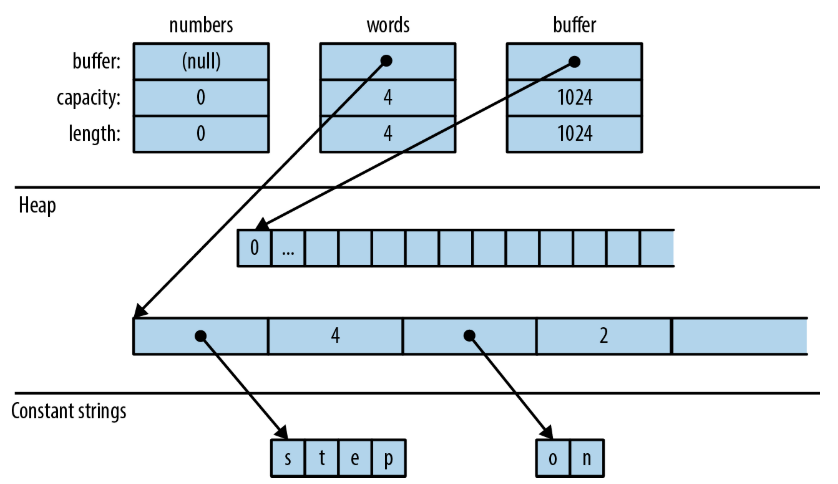
\includegraphics[width=0.9\textwidth]{../img/f16-1.png}
    \caption{vector的内存布局：words的每个元素是一个由指针和长度组成的\&str值}
    \label{f16-1}
\end{figure}

类似于所有集合，\texttt{Vec}实现了\texttt{std::iter::FromIterator}，因此你可以对任何迭代器调用\texttt{.collect()}方法来创建一个vector，正如“\nameref{BuildColl}”中所述：
\begin{minted}{Rust}
    // 将一个其他集合转换成vector
    let my_vec = my_set.into_iter().collect::<Vec<String>>();
\end{minted}

\subsection{访问元素}
通过索引访问数组、切片或vector的元素非常直观：
\begin{minted}{Rust}
    // 获取一个元素的引用
    let first_line = &lines[0];

    // 获取一个元素的拷贝 
    let fifth_number = numbers[4];          // 需要Copy
    let second_number = lines[1].clone();   // 需要Clone

    // 获取一个切片的引用
    let my_ref = &buffer[4..12];

    // 获取一个切片的拷贝
    let my_copy = buffer[4..12].to_vec();   // 需要Clone
\end{minted}

当索引越界时所有这些方式都会panic。

Rust对数字类型很挑剔，vector也不例外。vector的长度和索引都是\texttt{usize}类型。尝试使用\texttt{u32}、\texttt{u64}、\texttt{isize}作为vector的索引会导致错误。必要时你可以使用\texttt{n as usize}来转换，见“\nameref{cast}”。

有几种方法提供了便捷地访问vector或切片的特定元素的方法（注意所有的切片方法都能用于数组和vector）：
\codeentry{slice.first()}
\hangparagraph{返回\texttt{slice}的第一个元素的引用。返回类型是\texttt{Option<\&T>}，因此如果\texttt{slice}为空时返回值为\texttt{None}，不为空时返回值为\texttt{Some(\&slice[0])}}：
\begin{minted}{Rust}
    if let Some(item) = v.first() {
        println!("We got one! {}", item);
    }
\end{minted}

\codeentry{slice.last()}
\hangparagraph{和上边相似，不过返回最有一个元素的引用。}

\codeentry{slice.get(index)}
\hangparagraph{返回\texttt{slice[index]}的引用，如果存在的话。如果\texttt{slice}的元素数量小于\texttt{index+1}，那么返回\texttt{None}}：
\begin{minted}{Rust}
    let slice = [0, 1, 2, 3];
    assert_eq!(slice.get(2), Some(&2));
    assert_eq!(slice.get(4), None);
\end{minted}

\codeentry{slice.first\_mut(), slice.last\_mut(), slice.get\_mut(index)}
\hangparagraph{与上面的类似，不过借用\texttt{mut}引用：}
\begin{minted}{Rust}
    let mut slice = [0, 1, 2, 3];
    {
        let last = slice.last_mut().unwrap();   // 最后一个元素类型：&mut i32
        assert_eq!(*last, 3);
        *last = 100;
    }
\end{minted}

因为以值返回\texttt{T}意味着移动它，因此访问元素的方法通常返回元素的引用。

一个例外是\texttt{.to\_vec()}方法，它获取拷贝：

\codeentry{slice.to\_vec()}
\hangparagraph{克隆整个切片，返回一个新的vector：}
\begin{minted}{Rust}
    let v = [1, 2, 3, 4, 5, 6, 7, 8, 9];
    assert_eq!(v.to_vec(),
               vec![1, 2, 3, 4, 5, 6, 7, 8, 9]);
    assert_eq!(v[0..6].to_vec(),
               vec![1, 2, 3, 4, 5, 6]);
\end{minted}
\hangparagraph{只有当元素可以拷贝时这个方法才可用，即\texttt{where T: Clone}}

\subsection{迭代}


\chapter{字符串与文本}\label{ch17}

\emph{The string is a stark data structure and everywhere it is passed there is much duplication of process. It is a perfect vehicle for hiding information.}
\begin{flushright}
    ——Alan Perlis, epigram \#34
\end{flushright}

我们已经使用过了Rust中的主要文本类型：\texttt{String}、\texttt{str}和\texttt{char}。在\nameref{string}中，我们介绍了字符和字符串字面量的语法并且展示了字符串在内存中如何表示。在本章中，我们将更加详细地介绍文本。

在本章中：
\begin{enumerate}
    \item 我们会提供一些Unicode的背景知识，帮助你更好地理解标准库的设计。
    \item 我们会介绍\texttt{char}类型，它表示单个Unicode码点。
    \item 我们会介绍\texttt{String}和\texttt{str}类型，它们表示有所有权的和借用的Unicode字符序列。它们有非常多的方法用于构建、搜索、修改、迭代它们的内容。
    \item 我们会介绍Rust的字符串格式化设施，例如\texttt{println!}和\texttt{format!}宏。你可以编写自己的用于字符串格式化的宏，以及扩展它们来支持你自定义的类型。
    \item 我们会给出Rust中正则表达式支持的一个概述。
    \item 最后我们会讨论为什么Unicode规范化很重要，并展示如何在Rust中实现它。
\end{enumerate}

\section{Unicode背景知识}

本书是关于Rust的，而不是关于Unicode的，事实上已经有整本专门介绍它的书了。但Rust的字符和字符串类型被设计为Unicode。这里有一些有助于理解Rust的Unicode知识。

\subsection{ASCII、Latin-1和Unicode}

在所有ASCII码点范围（\texttt{0}到\texttt{0x7f}）内Unicode和ASCII完全相同：例如，这两种编码中字符\texttt{*}都是码点\texttt{42}。类似的，Unicode把\texttt{0}到\texttt{0xff}分配给与ISO/IEC 8859-1字符集相同的字符，这个字符集是ASCII的八位超集，用于西欧语言。Unicode把这个码点范围称为Latin-1代码块，因此我们采用更有表现力的名称Latin-1来指代ISO/IEC 8859-1。

由于Unicode是Latin-1的超集，把Latin-1转换为Unicode甚至不需要一张表：
\begin{minted}{Rust}
    fn latin1_to_char(latin1: u8) -> char {
        latin1 as char
    }
\end{minted}

反向转换同样很简单，前提是码点落在Latin-1的范围内：
\begin{minted}{Rust}
    fn char_to_latin1(c: char) -> Option<u8> {
        if c as u32 <= 0xff {
            Some(c as u8)
        } else {
            None
        }
    }
\end{minted}

\subsection{UTF-8}\label{utf8}

Rust的\texttt{String}和\texttt{str}类型使用UTF-8编码形式来表示文本。UTF-8把一个字符编码为一个一到四字节的序列（图\hyperref[f17-1]{17-1}）。

\begin{figure}[htbp]
    \centering
    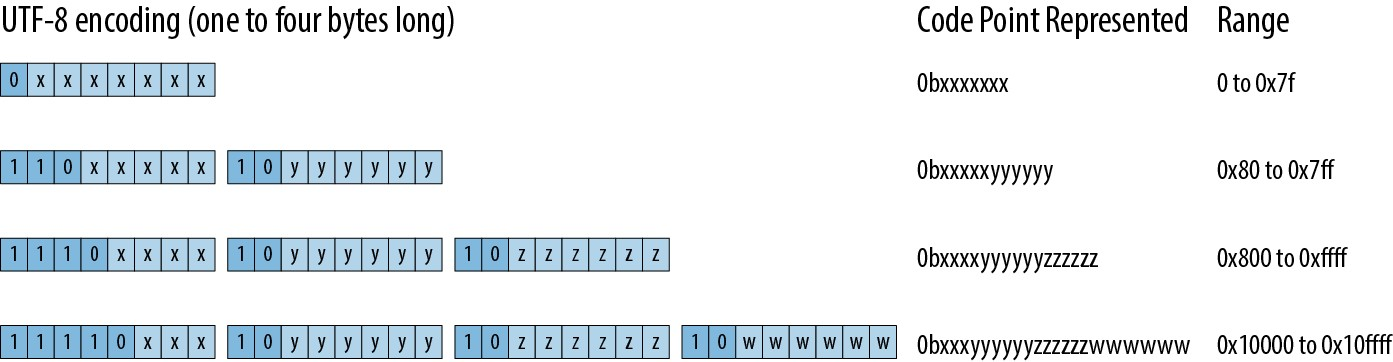
\includegraphics[width=0.8\textwidth]{../img/f17-1.jpg}
    \caption{UTF-8编码}
    \label{f17-1}
\end{figure}

对于良构的（well-formed）UTF-8序列有两条限制。第一，任何给定的码点只有最短的编码被认为是良构的；你不能用四个字节去编码一个只需要三个字节就能表示的码点。这条规则确保了一个给定的码点有且仅有一种UTF-8编码。第二，良构的UTF-8不能编码\texttt{0xd800}到\texttt{0xdfff}或者超过\texttt{0x10ffff}的数字：这些数字要么被保留用于非字符目的，要么完全超出了Unicode的范围。

图\hyperref[f17-2]{17-2}展示了一些例子。

\begin{figure}[htbp]
    \centering
    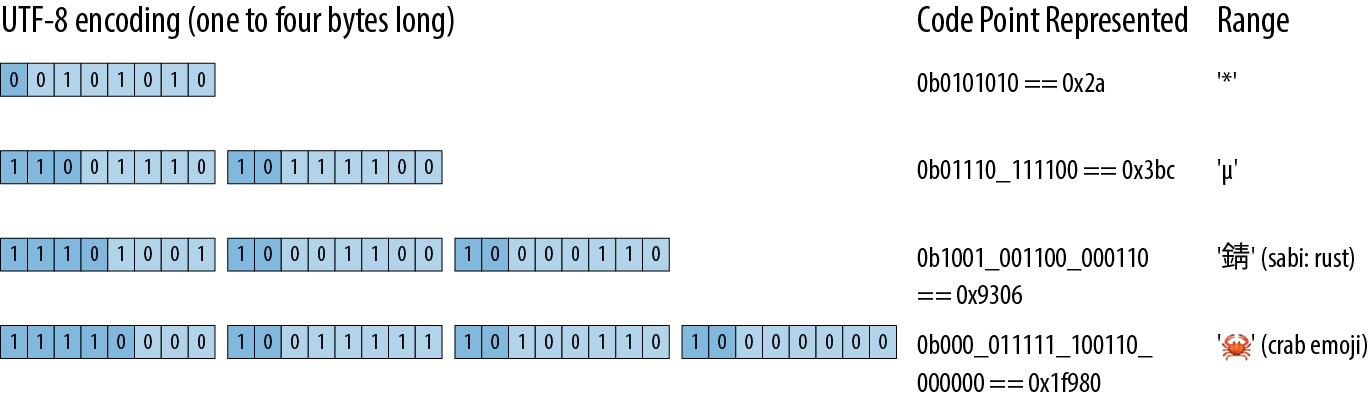
\includegraphics[width=0.8\textwidth]{../img/f17-2.jpg}
    \caption{UTF-8示例}
    \label{f17-2}
\end{figure}

注意，即使螃蟹emoji有一个首字节只给码点贡献了零的编码，它仍然需要一个四字节的编码：三字节的UTF-8编码只能表示16位的码点，而\texttt{0x1f980}有17位长。

下面是一个包含不同长度编码的字符的字符串示例：
\begin{minted}{Rust}
    assert_eq!("うどん: udon".as_bytes(),
               &[0xe3, 0x81, 0x86, // う
                 0xe3, 0x81, 0xa9, // ど
                 0xe3, 0x82, 0x93, // ん
                 0x3a, 0x20, 0x75, 0x64, 0x6f, 0x6e // : udon
               ]);
\end{minted}

图\hyperref[f17-2]{17-2}还展示了一些UTF-8非常有用的特性：
\begin{itemize}
    \item 由于UTF-8把\texttt{0}到\texttt{0x7f}的码点编码为恰好是\texttt{0}到\texttt{0x7f}的字节，因此持有ASCII文本的字节范围是有效的UTF-8。而且如果一段UTF-8字符串只包含ASCII字符，那么反过来也成立：它的UTF-8编码也是有效的ASCII。

    对于Latin-1则不成立：例如，Latin-1把é编码为字节\texttt{0xe9}，而UTF-8会把\texttt{0xe9}解释为某个三字节编码的第一个字节。
    \item 通过查看任意字节的高位，你可以立即判断出它是某个字符的UTF-8编码的开头，还是该编码中间的某个字节。
    \item 仅凭一个编码的首字节，通过它的前导位就能知道编码的完整长度。
    \item 由于没有编码长于四个字节，UTF-8处理永远不需要无界循环，这在处理不可信数据时非常方便。
    \item 在良构的UTF-8中，即使你从字节序列中间的任意位置开始，也总能明确地判断出字符编码在哪里开始、在哪里结束。UTF-8的首字节和后续字节总是可以区分的，因此一个编码不可能在另一个编码的中间开始。首字节决定了编码的总长度，因此没有任何编码是另一个编码的前缀。这带来很多不错的结果。例如，在UTF-8字符串中搜索一个ASCII分隔符字符只需要简单扫描分隔符的字节即可。它永远不会作为任何多字节编码的一部分出现，所以完全不需要跟踪UTF-8的结构。类似地，在一个字节串中搜索另一个字节串的算法，可以直接用于UTF-8字符串而不需要任何修改，即使有些算法并不会检查被搜索文本的每一个字节。
\end{itemize}

虽然可变宽度的编码比固定宽度的编码更复杂，但正是这些特性让UTF-8比你可能预期的更加易于使用。标准库为你处理了大多数方面。

\subsection{文本方向}

像拉丁、西里尔和泰语这样的文字是从左到右书写的，而希伯来语和阿拉伯语等其他文字则是从右到左书写的。Unicode按照文本通常书写或阅读的顺序存储字符，因此持有（比如说）希伯来文本的字符串的起始字节编码的是会写在最右边的那个字符：
\begin{minted}{Rust}
    assert_eq!("טוב ערב".chars().next(), Some('ע'));
\end{minted}
\section{字符(\texttt{char})}

一个Rust的\texttt{char}是一个持有Unicode码点的32位值。\texttt{char}被保证落在\texttt{0}到\texttt{0xd7ff}或\texttt{0xe000}到\texttt{0x10ffff}的范围内；所有创建和操作\texttt{char}值的方法都确保这一点成立。\texttt{char}类型实现了\texttt{Copy}和\texttt{Clone}，以及所有通常用于比较、哈希和格式化的trait。

字符串切片可以用\texttt{slice.chars()}产生一个遍历其字符的迭代器：
\begin{minted}{Rust}
    assert_eq!("カニ".chars().next(), Some('カ'));
\end{minted}

在下面的描述中，变量\texttt{ch}的类型始终是\texttt{char}。

\subsection{字符分类}

\texttt{char}类型有把字符划分为几个常见类别的方法，如表\hyperref[t17-1]{17-1}所列。它们都依据Unicode中的定义。

\begin{longtable}{p{0.22\textwidth}p{0.3\textwidth}p{0.38\textwidth}}
    \caption{\texttt{char}类型的分类方法}
    \label{t17-1}\\
    \hline
    \textbf{方法} & \textbf{说明} & \textbf{示例} \\
    \hline
    \texttt{ch.is\_numeric()} & 数字字符。包括Unicode通用类别“Number; digit”和“Number; letter”，但不包括“Number; other”。 &
    \makecell[l]{\texttt{'4'.is\_numeric()}\\ \texttt{'四'.is\_numeric()}\\ \texttt{'⑧'.is\_numeric()}} \\
    \hline
    \rowcolor{tablecolor}
    \texttt{ch.is\_alphabetic()} & 字母字符：Unicode的“Alphabetic”派生属性。 &
    \makecell[l]{\texttt{'q'.is\_alphabetic()}\\ \texttt{'七'.is\_alphabetic()}} \\
    \hline
    \makecell[l]{\texttt{ch.is\_}\\ \texttt{alphanumeric()}} & 数字或字母，如前所述。 &
    \makecell[l]{\texttt{'9'.is\_alphanumeric()}\\ \texttt{'饂'.is\_alphanumeric()}\\ \texttt{!'*'.is\_alphanumeric()}} \\
    \hline
    \rowcolor{tablecolor}
    \texttt{ch.is\_whitespace()} & 空白字符：Unicode字符属性“WSpace=Y”。 &
    \makecell[l]{\texttt{' '.is\_whitespace()}\\ \texttt{'\textbackslash n'.is\_whitespace()}\\ \texttt{'\textbackslash u\{A0\}'.is\_whitespace()}} \\
    \hline
    \texttt{ch.is\_control()} & 控制字符：Unicode的“Other, control”通用类别。 &
    \makecell[l]{\texttt{'\textbackslash n'.is\_control()}\\ \texttt{'\textbackslash u\{85\}'.is\_control()}} \\
    \hline
\end{longtable}

一组与之平行的方法只限于ASCII，对任何非ASCII的\texttt{char}都返回false（表\hyperref[t17-2]{17-2}）。

\begin{longtable}{p{0.24\textwidth}p{0.3\textwidth}p{0.36\textwidth}}
    \caption{\texttt{char}类型的ASCII分类方法}
    \label{t17-2}\\
    \hline
    \textbf{方法} & \textbf{说明} & \textbf{示例} \\
    \hline
    \texttt{ch.is\_ascii()} & 一个ASCII字符：码点在\texttt{0}到\texttt{127}（含）之间。 &
    \makecell[l]{\texttt{'n'.is\_ascii()}\\ \texttt{!'ñ'.is\_ascii()}} \\
    \rowcolor{tablecolor}
    \makecell[l]{\texttt{ch.is\_ascii\_}\\ \texttt{alphabetic()}} & 大写或小写的ASCII字母，在\texttt{'A'..='Z'}或\texttt{'a'..='z'}范围内。 &
    \makecell[l]{\texttt{'n'.is\_ascii\_alphabetic()}\\ \texttt{!'1'.is\_ascii\_alphabetic()}\\ \texttt{!'ñ'.is\_ascii\_alphabetic()}} \\
    \texttt{ch.is\_ascii\_digit()} & 一个ASCII数字，在\texttt{'0'..='9'}范围内。 &
    \makecell[l]{\texttt{'8'.is\_ascii\_digit()}\\ \texttt{!'-'.is\_ascii\_digit()}\\ \texttt{!'⑧'.is\_ascii\_digit()}} \\
    \rowcolor{tablecolor}
    \makecell[l]{\texttt{ch.is\_ascii\_}\\ \texttt{hexdigit()}} & \texttt{'0'..='9'}、\texttt{'A'..='F'}或\texttt{'a'..='f'}范围内的任意字符。 & \\
    \makecell[l]{\texttt{ch.is\_ascii\_}\\ \texttt{alphanumeric()}} & 一个ASCII数字或大写或小写字母。 &
    \makecell[l]{\texttt{'q'.is\_ascii\_alphanumeric()}\\ \texttt{'0'.is\_ascii\_alphanumeric()}} \\
    \rowcolor{tablecolor}
    \texttt{ch.is\_ascii\_control()} & 一个ASCII控制字符，包括“DEL”。 &
    \makecell[l]{\texttt{'\textbackslash n'.is\_ascii\_control()}\\ \texttt{'\textbackslash x7f'.is\_ascii\_control()}} \\
    \texttt{ch.is\_ascii\_graphic()} & 任何在页面上留下墨迹的ASCII字符：既不是空格也不是控制字符。 &
    \makecell[l]{\texttt{'Q'.is\_ascii\_graphic()}\\ \texttt{'\textasciitilde{}'.is\_ascii\_graphic()}\\ \texttt{!' '.is\_ascii\_graphic()}} \\
    \rowcolor{tablecolor}
    \makecell[l]{\texttt{ch.is\_ascii\_}\\ \texttt{uppercase(),}\\ \texttt{ch.is\_ascii\_}\\ \texttt{lowercase()}} & ASCII大写和小写字母。 &
    \makecell[l]{\texttt{'z'.is\_ascii\_lowercase()}\\ \texttt{'Z'.is\_ascii\_uppercase()}} \\
    \makecell[l]{\texttt{ch.is\_ascii\_}\\ \texttt{punctuation()}} & 既不是字母也不是数字的ASCII图形字符。 & \\
    \rowcolor{tablecolor}
    \makecell[l]{\texttt{ch.is\_ascii\_}\\ \texttt{whitespace()}} & 一个ASCII空白字符：空格、水平制表符、换行符、换页符或回车符。 &
    \makecell[l]{\texttt{' '.is\_ascii\_whitespace()}\\ \texttt{'\textbackslash n'.is\_ascii\_whitespace()}\\ \texttt{!'\textbackslash u\{A0\}'.is\_ascii\_whitespace()}} \\
    \hline
\end{longtable}

所有的\texttt{is\_ascii\_...}方法在\texttt{u8}字节类型上也可以使用：
\begin{minted}{Rust}
    assert!(32u8.is_ascii_whitespace());
    assert!(b'9'.is_ascii_digit());
\end{minted}

在把这些函数用于实现现有的规范（比如某种编程语言的标准或文件格式）时要小心，因为分类可能有令人惊讶的差异。例如，注意\texttt{is\_whitespace}和\texttt{is\_ascii\_whitespace}对某些字符的处理是不同的：
\begin{minted}{Rust}
    let line_tab = '\u{000b}'; // 'line tab'，也叫'vertical tab'（垂直制表符）
    assert_eq!(line_tab.is_whitespace(), true);
    assert_eq!(line_tab.is_ascii_whitespace(), false);
\end{minted}

\texttt{char::is\_ascii\_whitespace}函数实现的是许多Web标准通用的空白字符定义，而\texttt{char::is\_whitespace}遵循的是Unicode标准。

\subsection{处理数字}

对于处理数字，你可以使用下面的方法：

\codeentry{ch.to\_digit(radix)}
\hangparagraph{判断\texttt{ch}是不是\texttt{radix}进制中的数字。如果是，返回\texttt{Some(num)}，其中\texttt{num}是一个\texttt{u32}；否则返回\texttt{None}。它只识别ASCII数字，而不识别\texttt{char::is\_numeric}覆盖的更广泛的字符类别。\texttt{radix}参数的范围可以是2到36。对于大于10的进制，两种大小写的ASCII字母都被视为数字，值从10到35。}

\codeentry{std::char::from\_digit(num, radix)}
\hangparagraph{一个自由函数，如果可能的话，把\texttt{u32}数字值\texttt{num}转换为\texttt{char}。如果\texttt{num}可以表示为\texttt{radix}进制中的一个数字，\texttt{from\_digit}返回\texttt{Some(ch)}，其中\texttt{ch}就是这个数字；当\texttt{radix}大于10时，\texttt{ch}可能是小写字母。否则返回\texttt{None}。}

\hangparagraph{这是\texttt{to\_digit}的逆操作。如果\texttt{std::char::from\_digit(num, radix)}是\texttt{Some(ch)}，那么\texttt{ch.to\_digit(radix)}就是\texttt{Some(num)}。如果\texttt{ch}是一个ASCII数字或小写字母，那么反过来也成立。}

\codeentry{ch.is\_digit(radix)}
\hangparagraph{如果\texttt{ch}是\texttt{radix}进制中的一个ASCII数字，返回\texttt{true}。这等价于\texttt{ch.to\_digit(radix) != None}。}


所以，例如：

\begin{minted}{Rust}
    assert_eq!('F'.to_digit(16), Some(15));
    assert_eq!(std::char::from_digit(15, 16), Some('f'));
    assert!(char::is_digit('f', 16));
\end{minted}

\subsection{字符大小写转换}\label{CaseConv}

对于处理字符大小写：

\codeentry{ch.is\_lowercase(), ch.is\_uppercase()}
\hangparagraph{指示\texttt{ch}是小写还是大写字母字符。它们遵循Unicode的Lowercase和Uppercase派生属性，因此覆盖希腊语和西里尔语等非拉丁字母，并对ASCII给出预期的结果。}

\codeentry{ch.to\_lowercase(), ch.to\_uppercase()}
\hangparagraph{返回产生\texttt{ch}的小写和大写等价字符的迭代器，依据Unicode默认大小写转换算法：}
\begin{minted}{Rust}
    let mut upper = 's'.to_uppercase();
    assert_eq!(upper.next(), Some('S'));
    assert_eq!(upper.next(), None);
\end{minted}

\hangparagraph{这些方法返回一个迭代器而不是单个字符，因为Unicode中的大小写转换并不总是一对一的过程：}
\begin{minted}{Rust}
    // 德语字母"sharp S"的大写形式是"SS"：
    let mut upper = 'ß'.to_uppercase();
    assert_eq!(upper.next(), Some('S'));
    assert_eq!(upper.next(), Some('S'));
    assert_eq!(upper.next(), None);

    // Unicode规定把土耳其语带点的首都'İ'转小写为'i'
    // 后面跟着`'\u{307}'`（COMBINING DOT ABOVE，上方组合点），
    // 这样之后再次转回大写时可以保留这个点。
    let ch = 'İ'; // `'\u{130}'`
    let mut lower = ch.to_lowercase();
    assert_eq!(lower.next(), Some('i'));
    assert_eq!(lower.next(), Some('\u{307}'));
    assert_eq!(lower.next(), None);
\end{minted}

\hangparagraph{为了方便，这些迭代器实现了\texttt{std::fmt::Display} trait，所以你可以把它们直接传给\texttt{println!}或\texttt{write!}宏。}

\subsection{与整数之间的转换}

Rust的\texttt{as}运算符可以把\texttt{char}转换为任何整数类型，静默地截断任何高位的比特：
\begin{minted}{Rust}
    assert_eq!('B' as u32, 66);
    assert_eq!('饂' as u8, 66);   // 高位比特被截断
    assert_eq!('二' as i8, -116); // 同上
\end{minted}

\texttt{as}运算符可以把任何\texttt{u8}值转换为\texttt{char}，\texttt{char}也实现了\texttt{From<u8>}，但更宽的整数类型可以表示无效的码点，所以对于这些类型你必须使用\texttt{std::char::from\_u32}，它返回\texttt{Option<char>}：
\begin{minted}{Rust}
    assert_eq!(char::from(66), 'B');
    assert_eq!(std::char::from_u32(0x9942), Some('饂'));
    assert_eq!(std::char::from_u32(0xd800), None); // 保留给UTF-16
\end{minted}
\section{\texttt{String}和\texttt{str}}

Rust的\texttt{String}和\texttt{str}类型被保证只持有良构的（well-formed）UTF-8。库通过限制你创建\texttt{String}和\texttt{str}值的方式以及你可以对它们执行的操作来确保这一点，使得值在被引入时是良构的，并且在你使用它们的过程中保持良构。它们的所有方法都保护这一保证：没有任何安全操作可以在它们上引入不良构的UTF-8。这简化了处理文本的代码。

Rust根据方法是否需要可调整大小的缓冲区，或者是否满足于就地使用文本，把文本处理方法放在\texttt{str}或\texttt{String}上。由于\texttt{String}解引用到\texttt{\&str}，在\texttt{str}上定义的每个方法都可以直接在\texttt{String}上使用。本节呈现来自两种类型的方法，按大致功能分组。

这些方法按字节偏移量索引文本，并按字节而非字符测量其长度。实际上，考虑到Unicode的性质，按字符索引并不像看起来那么有用，而字节偏移量更快、更简单。如果你试图使用一个落在某个字符的UTF-8编码中间的字节偏移量，方法会panic，所以你无法用这种方式引入不良构的UTF-8。

\texttt{String}被实现为\texttt{Vec<u8>}的一个包装器，确保vector的内容总是良构的UTF-8。Rust永远不会改变\texttt{String}去使用更复杂的表示，所以你可以假设\texttt{String}具有与\texttt{Vec}相同的性能特征。

在这些解释中，变量具有表\hyperref[t17-3]{17-3}中给出的类型。

\begin{longtable}{p{0.18\textwidth}p{0.72\textwidth}}
    \caption{解释中所用变量的类型}
    \label{t17-3}\\
    \hline
    \textbf{变量} & \textbf{假定的类型} \\
    \hline
    \texttt{string} & \texttt{String} \\
    \hline
    \rowcolor{tablecolor}
    \texttt{slice} & \texttt{\&str}，或任何解引用为\texttt{\&str}的类型，比如\texttt{String}或\texttt{Rc<String>} \\
    \hline
    \texttt{ch} & \texttt{char} \\
    \hline
    \rowcolor{tablecolor}
    \texttt{n} & \texttt{usize}，一个长度 \\
    \hline
    \texttt{i, j} & \texttt{usize}，一个字节偏移量 \\
    \hline
    \rowcolor{tablecolor}
    \texttt{range} & 一个\texttt{usize}字节偏移量的范围，可以是像\texttt{i..j}这样完全有界的，或像\texttt{i..}、\texttt{..j}或\texttt{..}这样部分有界的 \\
    \hline
    \texttt{pattern} & 任何模式类型：\texttt{char}、\texttt{String}、\texttt{\&str}、\texttt{\&[char]}或\texttt{FnMut(char) -> bool} \\
    \hline
\end{longtable}

我们在\nameref{Patterns}中描述模式类型。

\subsection{创建\texttt{String}值}

有几种常见的方法可以创建\texttt{String}值：

\codeentry{String::new()}
\hangparagraph{返回一个新的空字符串。它没有堆分配的缓冲区，但会按需分配一个。}

\codeentry{String::with\_capacity(n)}
\hangparagraph{返回一个新的空字符串，其缓冲区被预先分配以容纳至少\texttt{n}个字节。如果你事先知道要构建的字符串的长度，这个构造函数让你从一开始就把缓冲区大小调整正确，而不是在构建字符串的过程中调整缓冲区大小。如果字符串的长度超过\texttt{n}个字节，字符串仍然会按需增长其缓冲区。和vector一样，字符串有\texttt{capacity}、\texttt{reserve}和\texttt{shrink\_to\_fit}方法，但通常默认的分配逻辑就足够了。}

\codeentry{str\_slice.to\_string()}
\hangparagraph{分配一个新的\texttt{String}，其内容是\texttt{str\_slice}的副本。我们已经在整本书中一直使用像\texttt{"literal text".to\_string()}这样的表达式来从字符串字面量创建\texttt{String}。}

\codeentry{iter.collect()}
\hangparagraph{通过连接迭代器的条目来构造一个字符串，这些条目可以是\texttt{char}、\texttt{\&str}或\texttt{String}值。例如，要删除字符串中的所有空格，你可以写：}
\begin{minted}{Rust}
    let spacey = "man hat tan";
    let spaceless: String =spacey.chars().filter(|c| !c.is_whitespace()).collect();
    assert_eq!(spaceless, "manhattan");
\end{minted}

\hangparagraph{这样使用\texttt{collect}利用了\texttt{String}对\texttt{std::iter::FromIterator} trait的实现。}

\codeentry{slice.to\_owned()}
\hangparagraph{返回\texttt{slice}的副本，作为一个新分配的\texttt{String}。\texttt{str}类型不能实现\texttt{Clone}：该trait会要求对\texttt{\&str}调用\texttt{clone}返回一个\texttt{str}值，但\texttt{str}是unsized的。不过，\texttt{\&str}确实实现了\texttt{ToOwned}，它允许实现者指定其有所有权的等价类型。}

\subsection{简单的查看方法}

这些方法从字符串切片获得基本信息：

\codeentry{slice.len()}
\hangparagraph{\texttt{slice}的长度，以字节为单位。}

\codeentry{slice.is\_empty()}
\hangparagraph{如果\texttt{slice.len() == 0}则为\texttt{true}。}

\codeentry{slice[range]}
\hangparagraph{返回借用\texttt{slice}的给定部分的切片。部分有界和无界的范围都可以；例如：}
\begin{minted}{Rust}
    let full = "bookkeeping";
    assert_eq!(&full[..4], "book");
    assert_eq!(&full[5..], "eeping");
    assert_eq!(&full[2..4], "ok");
    assert_eq!(full[..].len(), 11);
    assert_eq!(full[5..].contains("boo"), false);
\end{minted}

\hangparagraph{注意你不能用单个位置索引字符串切片，比如\texttt{slice[i]}。在给定的字节偏移量处获取单个字符有点笨拙：你必须对切片产生一个\texttt{chars}迭代器，并要求它解析一个字符的UTF-8：}
\begin{minted}{Rust}
    let parenthesized = "Rust (饂)";
    assert_eq!(parenthesized[6..].chars().next(), Some('饂'));
\end{minted}

\hangparagraph{不过，你应该很少需要这样做。Rust有更好的方式来迭代切片，我们将在\nameref{IterText}中描述。}

\codeentry{slice.split\_at(i)}
\hangparagraph{返回从\texttt{slice}借用的两个共享切片的元组：字节偏移量\texttt{i}之前的部分，以及它之后的部分。换句话说，这返回\texttt{(slice[..i], slice[i..])}。}

\codeentry{slice.is\_char\_boundary(i)}
\hangparagraph{如果字节偏移量\texttt{i}落在字符边界之间，因此适合作为\texttt{slice}的偏移量，则为\texttt{true}。}

自然地，切片可以比较相等、排序和哈希。有序比较只是把字符串视为Unicode码点的序列，并按字典顺序比较它们。

\subsection{附加和插入文本}\label{AppendText}

下面的方法向\texttt{String}添加文本：

\codeentry{string.push(ch)}
\hangparagraph{把字符\texttt{ch}附加到\texttt{string}的末尾。}

\codeentry{string.push\_str(slice)}
\hangparagraph{附加\texttt{slice}的全部内容。}

\codeentry{string.extend(iter)}
\hangparagraph{把迭代器\texttt{iter}产生的条目附加到字符串中。迭代器可以产生\texttt{char}、\texttt{str}或\texttt{String}值。这些是\texttt{String}对\texttt{std::iter::Extend}的实现：}
\begin{minted}{Rust}
    let mut also_spaceless = "con".to_string();
    also_spaceless.extend("tri but ion".split_whitespace());
    assert_eq!(also_spaceless, "contribution");
\end{minted}

\codeentry{string.insert(i, ch)}
\hangparagraph{在\texttt{string}的字节偏移量\texttt{i}处插入单个字符\texttt{ch}。这需要把\texttt{i}之后的任何字符向后移动，为\texttt{ch}腾出空间，所以用这种方式构建字符串可能需要与字符串长度成二次方的时间。}

\codeentry{string.insert\_str(i, slice)}
\hangparagraph{这对\texttt{slice}做同样的事情，并有相同的性能警告。}

\texttt{String}实现了\texttt{std::fmt::Write}，这意味着\texttt{write!}和\texttt{writeln!}宏可以把格式化文本附加到\texttt{String}上：
\begin{minted}{Rust}
    use std::fmt::Write;

    let mut letter = String::new();
    writeln!(letter, "Whose {} these are I think I know", "rutabagas")?;
    writeln!(letter, "His house is in the village though;")?;
    assert_eq!(letter, "Whose rutabagas these are I think I know\n\
                        His house is in the village though;\n");
\end{minted}

由于\texttt{write!}和\texttt{writeln!}是为写入输出流而设计的，它们返回一个\texttt{Result}，如果你忽略它，Rust会抱怨。这段代码使用\texttt{?}运算符来处理它，但写入\texttt{String}实际上是不会失败的，所以在这种情况下调用\texttt{.unwrap()}也没问题。

由于\texttt{String}实现了\texttt{Add<\&str>}和\texttt{AddAssign<\&str>}，你可以写这样的代码：
\begin{minted}{Rust}
    let left = "partners".to_string();
    let mut right = "crime".to_string();
    assert_eq!(left + " in " + &right, "partners in crime");

    right += " doesn't pay";
    assert_eq!(right, "crime doesn't pay");
\end{minted}

当应用于字符串时，\texttt{+}运算符按值获取其左操作数，所以它实际上可以复用该\texttt{String}作为加法的结果。因此，如果左操作数的缓冲区足够大以容纳结果，就不需要分配。

一个不幸的不对称之处是，\texttt{+}的左操作数不能是\texttt{\&str}，所以你不能写：
\begin{minted}{Rust}
    let parenthetical = "(" + string + ")";
\end{minted}

你必须改写成：
\begin{minted}{Rust}
    let parenthetical = "(".to_string() + &string + ")";
\end{minted}

然而，这个限制确实不鼓励从末尾向前构建字符串。这种方法性能很差，因为文本必须被反复地向缓冲区末尾移动。

然而，从头到尾附加小块来构建字符串是高效的。\texttt{String}的行为和vector一样，当它需要更多容量时，总是至少把缓冲区的大小翻倍。这使重新复制的开销与最终大小成比例。即便如此，使用\texttt{String::with\_capacity}从一开始就以正确的缓冲区大小创建字符串，可以完全避免调整大小，并可以减少对堆分配器的调用次数。

\subsection{移除和替换文本}

\texttt{String}有一些移除文本的方法（这些方法不影响字符串的容量；如果你需要释放内存，使用\texttt{shrink\_to\_fit}）：

\codeentry{string.clear()}
\hangparagraph{把\texttt{string}重置为空字符串。}

\codeentry{string.truncate(n)}
\hangparagraph{丢弃字节偏移量\texttt{n}之后的所有字符，使\texttt{string}的长度最多为\texttt{n}。如果\texttt{string}短于\texttt{n}个字节，这没有效果。}

\codeentry{string.pop()}
\hangparagraph{从\texttt{string}移除最后一个字符（如果有的话），并把它作为\texttt{Option<char>}返回。}

\codeentry{string.remove(i)}
\hangparagraph{从\texttt{string}移除字节偏移量\texttt{i}处的字符并返回它，把后面的任何字符向前移动。这需要的时间与后面字符的数量成线性关系。}

\codeentry{string.drain(range)}
\hangparagraph{返回对给定字节索引范围的一个迭代器，并在迭代器被丢弃时移除这些字符。范围之后的字符被向前移动：}
\begin{minted}{Rust}
    let mut choco = "chocolate".to_string();
    assert_eq!(choco.drain(3..6).collect::<String>(), "col");
    assert_eq!(choco, "choate");
\end{minted}

\hangparagraph{如果你只想移除这个范围，你可以立即丢弃迭代器，而不从中提取任何条目：}

\begin{minted}{Rust}
    let mut winston = "Churchill".to_string();
    winston.drain(2..6);
    assert_eq!(winston, "Chill");
\end{minted}

\codeentry{string.replace\_range(range, replacement)}
\hangparagraph{用给定的替换字符串切片替换\texttt{string}中的给定范围。这个切片不必与要替换的范围长度相同，但除非被替换的范围一直延伸到\texttt{string}的末尾，否则这将需要移动范围末尾之后的所有字节：}
\begin{minted}{Rust}
    let mut beverage = "a piña colada".to_string();
    beverage.replace_range(2..7, "kahlua"); // 'ñ'是两个字节！
    assert_eq!(beverage, "a kahlua colada");
\end{minted}

\subsection{搜索和迭代的约定}

Rust标准库中用于搜索文本和迭代文本的函数遵循一些命名约定，使它们更容易记忆：
\begin{itemize}
    \item \texttt{r}：大多数操作从头到尾处理文本，但名称以\texttt{r}开头的操作从尾到头工作。例如，\texttt{rsplit}是\texttt{split}的从尾到头版本。在某些情况下，改变方向不仅会影响产生值的顺序，还会影响值本身。关于这个的例子见图\hyperref[f17-3]{17-3}。
    \item \texttt{n}：名称以\texttt{n}结尾的迭代器把自己限制在给定数量的匹配上。
    \item \texttt{\_indices}：名称以\texttt{\_indices}结尾的迭代器连同它们通常的迭代值一起产生它们在切片中出现的字节偏移量。
\end{itemize}

标准库并没有为每个操作提供所有组合。例如，许多操作不需要\texttt{n}变体，因为提前结束迭代很容易。

\subsection{搜索文本的模式}\label{Patterns}

当标准库函数需要搜索、匹配、分割或修剪文本时，它接受几种不同的类型来表示要查找的内容：
\begin{minted}{Rust}
    let haystack = "One fine day, in the middle of the night";

    assert_eq!(haystack.find(','), Some(12));
    assert_eq!(haystack.find("night"), Some(35));
    assert_eq!(haystack.find(char::is_whitespace), Some(3));
\end{minted}

这些类型被称为模式（pattern），大多数操作都支持它们：
\begin{minted}{Rust}
    assert_eq!("## Elephants"
               .trim_start_matches(|ch: char| ch == '#' || ch.is_whitespace()), "Elephants");
\end{minted}

标准库支持四种主要的模式：
\begin{itemize}
    \item 一个\texttt{char}作为模式匹配该字符。
    \item 一个\texttt{String}或\texttt{\&str}或\texttt{\&\&str}作为模式匹配与模式相等的子字符串。
    \item 一个\texttt{FnMut(char) -> bool}闭包作为模式匹配闭包返回\texttt{true}的单个字符。
    \item 一个\texttt{\&[char]}（不是\texttt{\&str}，而是一个\texttt{char}值的切片）作为模式匹配列表中出现的任何单个字符。注意，如果你把列表写成数组字面量，你可能需要调用\texttt{as\_ref()}来把类型弄对：
\begin{minted}{Rust}
    let code = "\t    function noodle() { ";
    assert_eq!(code.trim_start_matches([' ', '\t'].as_ref()), "function noodle() { ");
    // 更短的等价写法：&[' ', '\t'][..]
\end{minted}

    否则，Rust会被固定大小数组类型\texttt{\&[char; 2]}弄糊涂，它不幸地不是一个模式类型。
\end{itemize}

在库自己的代码中，一个模式是任何实现了\texttt{std::str::Pattern} trait的类型。\texttt{Pattern}的细节还不稳定，所以你不能在稳定版Rust中为你自己的类型实现它，但门是敞开的，以便将来允许正则表达式和其他复杂的模式。Rust确实保证现在支持的模式类型将来会继续工作。

\subsection{搜索和替换}

Rust有几个方法用于在切片中搜索模式，并可能用新文本替换它们：

\codeentry{slice.contains(pattern)}
\hangparagraph{如果\texttt{slice}包含\texttt{pattern}的一个匹配，返回\texttt{true}。}

\codeentry{slice.starts\_with(pattern), slice.ends\_with(pattern)}
\hangparagraph{如果\texttt{slice}的起始或结尾文本匹配\texttt{pattern}，返回\texttt{true}：}
\begin{minted}{Rust}
    assert!("2017".starts_with(char::is_numeric));
\end{minted}

\codeentry{slice.find(pattern), slice.rfind(pattern)}
\hangparagraph{如果\texttt{slice}包含\texttt{pattern}的一个匹配，返回\texttt{Some(i)}，其中\texttt{i}是模式出现的字节偏移量。\texttt{find}方法返回第一个匹配，\texttt{rfind}返回最后一个：}
\begin{minted}{Rust}
    let quip = "We also know there are known unknowns";
    assert_eq!(quip.find("know"), Some(8));
    assert_eq!(quip.rfind("know"), Some(31));
    assert_eq!(quip.find("ya know"), None);
    assert_eq!(quip.rfind(char::is_uppercase), Some(0));
\end{minted}

\codeentry{slice.replace(pattern, replacement)}
\hangparagraph{返回一个新的\texttt{String}，通过急切地（eagerly）用\texttt{replacement}替换\texttt{pattern}的所有匹配而形成：}
\begin{minted}{Rust}
    assert_eq!("The only thing we have to fear is fear itself"
               .replace("fear", "spin"),
               "The only thing we have to spin is spin itself");

    assert_eq!("`Borrow` and `BorrowMut`"
               .replace(|ch:char| !ch.is_alphanumeric(), ""),
               "BorrowandBorrowMut");
\end{minted}

\hangparagraph{因为替换是急切地完成的，\texttt{.replace()}在重叠匹配上的行为可能会令人惊讶。这里，模式\texttt{"aba"}有四个实例，但在第一个和第三个被替换后，第二个和第四个不再匹配：}
\begin{minted}{Rust}
    assert_eq!("cabababababbage".replace("aba", "***"),"c***b***babbage");
\end{minted}

\codeentry{slice.replacen(pattern, replacement, n)}
\hangparagraph{这做同样的事情，但最多替换前\texttt{n}个匹配。}

\subsection{迭代文本}\label{IterText}

标准库提供了几种迭代切片的文本的方式。图\hyperref[f17-3]{17-3}展示了一些例子。

你可以把\texttt{split}和\texttt{match}家族看作互为补充：split是匹配之间的范围。

\begin{figure}[htbp]
    \centering
    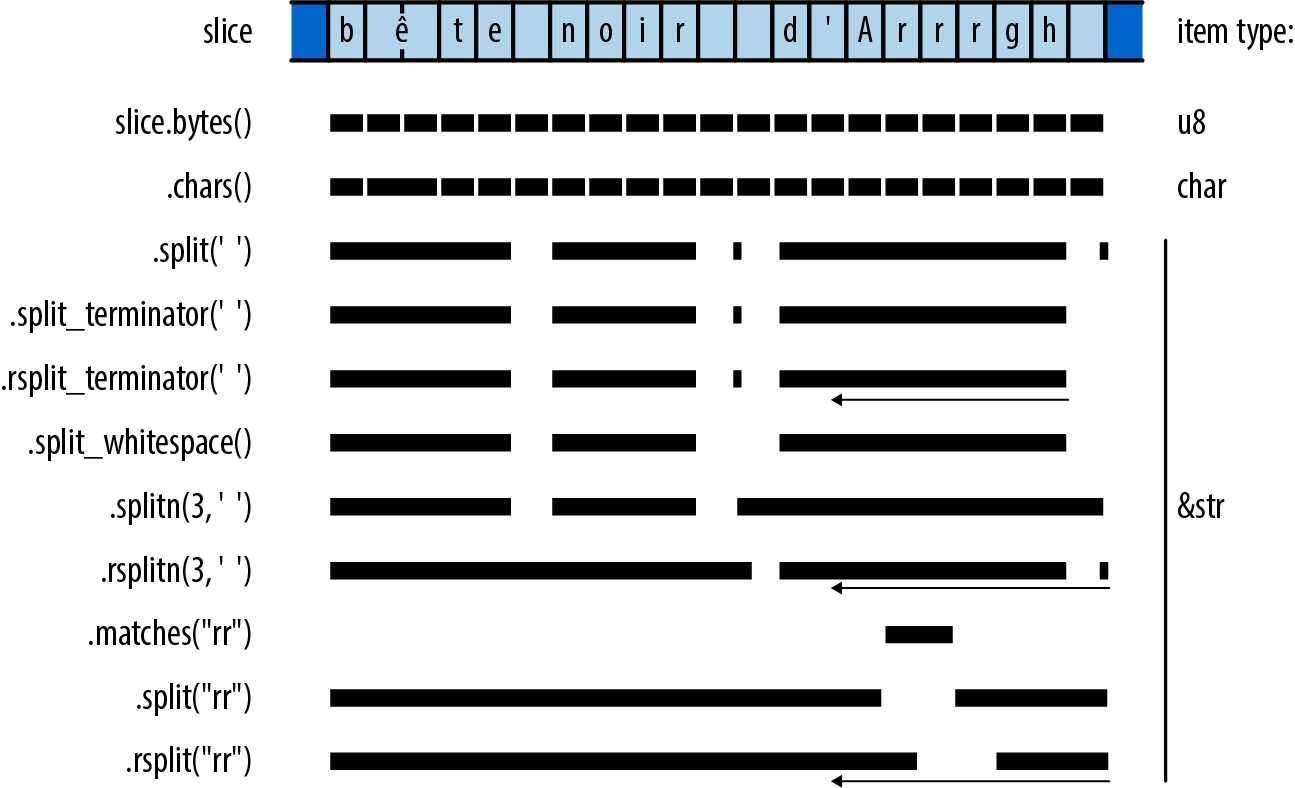
\includegraphics[width=0.8\textwidth]{../img/f17-3.jpg}
    \caption{在切片上迭代的一些方式}
    \label{f17-3}
\end{figure}

这些方法中的大多数返回可逆的迭代器（也就是说，它们实现了\texttt{DoubleEndedIterator}）：调用它们的\texttt{.rev()}适配器方法给你一个产生相同条目但顺序相反的迭代器。

\codeentry{slice.chars()}
\hangparagraph{返回遍历\texttt{slice}字符的迭代器。}

\codeentry{slice.char\_indices()}
\hangparagraph{返回遍历\texttt{slice}的字符及其字节偏移量的迭代器：}
\begin{minted}{Rust}
    assert_eq!("élan".char_indices().collect::<Vec<_>>(),
               vec![(0, 'é'), // 有一个两字节的UTF-8编码
                    (2, 'l'),
                    (3, 'a'),
                    (4, 'n')]);
\end{minted}

\hangparagraph{注意，这并不等同于\texttt{.chars().enumerate()}，因为它提供每个字符在\texttt{slice}内的字节偏移量，而不仅仅是给字符编号。}

\codeentry{slice.bytes()}
\hangparagraph{返回遍历\texttt{slice}的单个字节的迭代器，暴露UTF-8编码：}
\begin{minted}{Rust}
    assert_eq!("élan".bytes().collect::<Vec<_>>(),
               vec![195, 169, b'l', b'a', b'n']);
\end{minted}

\codeentry{slice.lines()}
\hangparagraph{返回遍历\texttt{slice}各行的迭代器。行以\texttt{"\textbackslash n"}或\texttt{"\textbackslash r\textbackslash n"}结束。产生的每个条目都是借用\texttt{slice}的\texttt{\&str}。这些条目不包括行的结束字符。}

\codeentry{slice.split(pattern)}
\hangparagraph{返回遍历\texttt{slice}被\texttt{pattern}的匹配分隔开的各个部分的迭代器。对于紧邻的匹配之间，以及\texttt{slice}开头和结尾处的匹配，这会产生空字符串。}

\hangparagraph{如果\texttt{pattern}是\texttt{\&str}，返回的迭代器不可逆。这样的模式根据你从哪个方向扫描可以产生不同的匹配序列，而可逆迭代器被禁止这样做。相反，你可能可以使用\texttt{rsplit}方法，接下来描述。}

\codeentry{slice.rsplit(pattern)}
\hangparagraph{这个方法相同，但是从尾到头扫描\texttt{slice}，按这个顺序产生匹配。}

\codeentry{slice.split\_terminator(pattern), slice.rsplit\_terminator(pattern)}
\hangparagraph{这些类似，但把\texttt{pattern}视为终止符而不是分隔符：如果\texttt{pattern}正好在\texttt{slice}的末尾匹配，迭代器不会产生一个表示该匹配与\texttt{slice}末尾之间空字符串的空切片，正如\texttt{split}和\texttt{rsplit}所做的那样。例如：}
\begin{minted}{Rust}
    // 这里的':'字符是分隔符。注意最后的""。
    assert_eq!("jimb:1000:Jim Blandy:".split(':').collect::<Vec<_>>(),
               vec!["jimb", "1000", "Jim Blandy", ""]);

    // 这里的'\n'字符是终止符。
    assert_eq!("127.0.0.1  localhost\n\
                127.0.0.1  www.reddit.com\n"
               .split_terminator('\n').collect::<Vec<_>>(),
               vec!["127.0.0.1  localhost",
                    "127.0.0.1  www.reddit.com"]);
               // 注意，没有最后的""！
\end{minted}

\codeentry{slice.splitn(n, pattern), slice.rsplitn(n, pattern)}
\hangparagraph{这些和\texttt{split}与\texttt{rsplit}类似，除了它们把字符串分割成最多\texttt{n}个切片，在\texttt{pattern}的前\texttt{n-1}个或后\texttt{n-1}个匹配处分割。}

\codeentry{slice.split\_whitespace(), slice.split\_ascii\_whitespace()}
\hangparagraph{返回遍历\texttt{slice}被空白分隔的各部分的迭代器。一段多个空白字符被视为单个分隔符。尾部的空白被忽略。}

\hangparagraph{\texttt{split\_whitespace}方法使用Unicode对空白的定义，正如\texttt{char}上的\texttt{is\_whitespace}方法所实现的。\texttt{split\_ascii\_whitespace}方法改用\texttt{char::is\_ascii\_whitespace}，它只识别ASCII空白字符。}
\begin{minted}{Rust}
    let poem = "This  is  just  to say\n\
                I have eaten\n\
                the plums\n\
                again\n";

    assert_eq!(poem.split_whitespace().collect::<Vec<_>>(),
               vec!["This", "is", "just", "to", "say",
                    "I", "have", "eaten", "the", "plums",
                    "again"]);
\end{minted}

\codeentry{slice.matches(pattern)}
\hangparagraph{返回遍历\texttt{slice}中\texttt{pattern}的匹配的迭代器。\texttt{slice.rmatches(pattern)}相同，但从尾到头迭代。}

\codeentry{slice.match\_indices(pattern), slice.rmatch\_indices(pattern)}
\hangparagraph{这些类似，除了产生的条目是\texttt{(offset, match)}对，其中\texttt{offset}是匹配开始的字节偏移量，\texttt{match}是匹配的切片。}

\subsection{修剪}

修剪字符串就是移除文本，通常是空白，从字符串的开头或结尾。在清理从文件读取的输入时通常很有用，用户可能为了可读性缩进了文本，或者无意中在一行末尾留下尾随空白。

\codeentry{slice.trim()}
\hangparagraph{返回\texttt{slice}的一个子切片，省略任何前导和尾随的空白。\texttt{slice.trim\_start()}只省略前导空白，\texttt{slice.trim\_end()}只省略尾随空白：}
\begin{minted}{Rust}
    assert_eq!("\t*.rs  ".trim(), "*.rs");
    assert_eq!("\t*.rs  ".trim_start(), "*.rs  ");
    assert_eq!("\t*.rs  ".trim_end(), "\t*.rs");
\end{minted}

\codeentry{slice.trim\_matches(pattern)}
\hangparagraph{返回\texttt{slice}的一个子切片，省略开头和结尾处\texttt{pattern}的所有匹配。\texttt{trim\_start\_matches}和\texttt{trim\_end\_matches}方法对只在前导或尾随匹配做同样的事情：}
\begin{minted}{Rust}
    assert_eq!("001990".trim_start_matches('0'), "1990");
\end{minted}

\subsection{字符串大小写转换}

方法\texttt{slice.to\_uppercase()}和\texttt{slice.to\_lowercase()}返回一个新分配的字符串，持有\texttt{slice}的文本转换后的大写或小写形式。结果可能与\texttt{slice}的长度不同；详情见\nameref{CaseConv}。
\subsection{从字符串解析其他类型}

Rust提供了从字符串解析值和产生值的文本表示的标准trait。

如果一个类型实现了\texttt{std::str::FromStr} trait，那么它提供了一种从字符串切片解析值的标准方式：
\begin{minted}{Rust}
    pub trait FromStr: Sized {
        type Err;
        fn from_str(s: &str) -> Result<Self, Self::Err>;
    }
\end{minted}

所有常用的机器类型都实现了\texttt{FromStr}：
\begin{minted}{Rust}
    use std::str::FromStr;

    assert_eq!(usize::from_str("3628800"), Ok(3628800));
    assert_eq!(f64::from_str("128.5625"), Ok(128.5625));
    assert_eq!(bool::from_str("true"), Ok(true));

    assert!(f64::from_str("not a float at all").is_err());
    assert!(bool::from_str("TRUE").is_err());
\end{minted}

\texttt{char}类型也实现了\texttt{FromStr}，用于只含一个字符的字符串：
\begin{minted}{Rust}
    assert_eq!(char::from_str("é"), Ok('é'));
    assert!(char::from_str("abcdefg").is_err());
\end{minted}

\texttt{std::net::IpAddr}类型，一个持有IPv4或IPv6互联网地址的枚举，也实现了\texttt{FromStr}：
\begin{minted}{Rust}
    use std::net::IpAddr;

    let address =
        IpAddr::from_str("fe80::0000:3ea9:f4ff:fe34:7a50")?;
    assert_eq!(address,
               IpAddr::from([0xfe80, 0, 0, 0, 0x3ea9, 0xf4ff, 0xfe34,
                             0x7a50]));
\end{minted}

字符串切片有一个\texttt{parse}方法，可以把切片解析为你喜欢的任何类型，前提是它实现了\texttt{FromStr}。和\texttt{Iterator::collect}一样，你有时需要写出你想要的具体类型，所以\texttt{parse}并不总是比直接调用\texttt{from\_str}更易读：
\begin{minted}{Rust}
    let address = "fe80::0000:3ea9:f4ff:fe34:7a50".parse::<IpAddr>()?;
\end{minted}

\subsection{把其他类型转换为字符串}

有三种主要的方式把非文本值转换为字符串：

\begin{itemize}
    \item 具有自然的人类可读打印形式的类型可以实现\texttt{std::fmt::Display} trait，它让你在\texttt{format!}宏中使用\texttt{\{\}}格式说明符：
\begin{minted}{Rust}
    assert_eq!(format!("{}, wow", "doge"), "doge, wow");
    assert_eq!(format!("{}", true), "true");
    assert_eq!(format!("({:.3}, {:.3})", 0.5, f64::sqrt(3.0)/2.0), "(0.500, 0.866)");

    // 使用上面的`address`。
    let formatted_addr: String = format!("{}", address);
    assert_eq!(formatted_addr, "fe80::3ea9:f4ff:fe34:7a50");
\end{minted}

    Rust的所有机器数值类型都实现\texttt{Display}，字符、字符串和切片也是如此。智能指针类型\texttt{Box<T>}、\texttt{Rc<T>}和\texttt{Arc<T>}在\texttt{T}本身实现\texttt{Display}时也实现\texttt{Display}：它们的显示形式就是其指向内容的显示形式。像\texttt{Vec}和\texttt{HashMap}这样的容器不实现\texttt{Display}，因为这些类型没有单一的自然人类可读形式。

    \item 如果一个类型实现了\texttt{Display}，标准库会自动为它实现\texttt{std::str::ToString} trait，当你不需要\texttt{format!}的灵活性时，其唯一的方法\texttt{to\_string}可能更方便：
\begin{minted}{Rust}
    // 继续上面的代码。
    assert_eq!(address.to_string(), "fe80::3ea9:f4ff:fe34:7a50");
\end{minted}

    \texttt{ToString} trait先于\texttt{Display}的引入，并且灵活性较低。对于你自己的类型，你通常应该实现\texttt{Display}而不是\texttt{ToString}。

    \item 标准库中的每个公共类型都实现了\texttt{std::fmt::Debug}，它以对程序员有帮助的方式把一个值格式化为字符串。使用\texttt{Debug}产生字符串的最简单方式是通过\texttt{format!}宏的\texttt{\{:?\}}格式说明符：
\begin{minted}{Rust}
    // 继续上面的代码。
    let addresses = vec![address,IpAddr::from_str("192.168.0.1")?];
    assert_eq!(format!("{:?}", addresses),"[fe80::3ea9:f4ff:fe34:7a50, 192.168.0.1]");
\end{minted}

    这利用了\texttt{Debug}对\texttt{Vec<T>}的覆盖性（blanket）实现，对任何本身实现\texttt{Debug}的\texttt{T}都成立。Rust的所有集合类型都有这样的实现。

    \item 你也应该为你自己的类型实现\texttt{Debug}。通常最好让Rust派生一个实现，正如我们在\hyperref[ch12]{第12章}中对\texttt{Complex}类型所做的那样：
\begin{minted}{Rust}
    #[derive(Copy, Clone, Debug)]
    struct Complex { re: f64, im: f64 }
\end{minted}
\end{itemize}

\texttt{Display}和\texttt{Debug}格式化trait只是\texttt{format!}宏及其同类用于把值格式化为文本的几个trait中的两个。我们将在\nameref{format}中介绍其他的，并解释如何全部实现它们。

\subsection{借用为其他文本类类型}

你可以用几种不同的方式借用切片的内容：

\begin{itemize}
    \item 切片和\texttt{String}实现\texttt{AsRef<str>}、\texttt{AsRef<[u8]>}、\texttt{AsRef<Path>}和\texttt{AsRef<OsStr>}。许多标准库函数使用这些trait作为其参数类型的约束，所以你可以直接把切片和字符串传给它们，即使它们真正想要的是某种其他类型。更详细的解释见\nameref{asref}。
    \item 切片和字符串也实现了\texttt{std::borrow::Borrow<str>} trait。\texttt{HashMap}和\texttt{BTreeMap}使用\texttt{Borrow}使\texttt{String}作为表中的键工作得很好。详情见\nameref{borrow}。
\end{itemize}

\subsection{以UTF-8的形式访问文本}

有两种主要的方式获取表示文本的字节，取决于你是想拥有字节还是只借用它们：

\codeentry{slice.as\_bytes()}
\hangparagraph{把\texttt{slice}的字节借用为\texttt{\&[u8]}。由于这不是可变引用，\texttt{slice}可以假设其字节将保持良构的UTF-8。}

\codeentry{string.into\_bytes()}
\hangparagraph{获取\texttt{string}的所有权，并按值返回字符串字节的\texttt{Vec<u8>}。这是一个廉价的转换，因为它只是交出\texttt{string}一直用作其缓冲区的那个\texttt{Vec<u8>}。由于\texttt{string}不再存在，这些字节不需要继续保持良构的UTF-8，调用者可以随意修改这个\texttt{Vec<u8>}。}

\subsection{从UTF-8数据产生文本}

如果你有一块你认为包含UTF-8数据的字节，你有几个选项把它们转换为\texttt{String}或切片，取决于你想如何处理错误：

\codeentry{str::from\_utf8(byte\_slice)}
\hangparagraph{取一个\texttt{\&[u8]}字节切片并返回一个\texttt{Result}：如果\texttt{byte\_slice}包含良构的UTF-8则返回\texttt{Ok(\&str)}，否则返回一个错误。}

\codeentry{String::from\_utf8(vec)}
\hangparagraph{尝试从一个按值传入的\texttt{Vec<u8>}构造一个字符串。如果\texttt{vec}持有良构的UTF-8，\texttt{from\_utf8}返回\texttt{Ok(string)}，其中\texttt{string}已经接管\texttt{vec}用作其缓冲区。不会发生堆分配或复制文本。}

\hangparagraph{如果字节不是有效的UTF-8，这返回\texttt{Err(e)}，其中\texttt{e}是一个\texttt{FromUtf8Error}错误值。调用\texttt{e.into\_bytes()}给你返回原来的vector \texttt{vec}，所以转换失败时它不会丢失：}
\begin{minted}{Rust}
    let good_utf8: Vec<u8> = vec![0xe9, 0x8c, 0x86];
    assert_eq!(String::from_utf8(good_utf8).ok(), Some("錆".to_string()));

    let bad_utf8:  Vec<u8> = vec![0x9f, 0xf0, 0xa6, 0x80];
    let result = String::from_utf8(bad_utf8);
    assert!(result.is_err());
    // 由于String::from_utf8失败了，它没有消耗原来的
    // vector，错误值把它毫发无损地交还给我们。
    assert_eq!(result.unwrap_err().into_bytes(), vec![0x9f, 0xf0, 0xa6, 0x80]);
\end{minted}

\codeentry{String::from\_utf8\_lossy(byte\_slice)}
\hangparagraph{尝试从一个\texttt{\&[u8]}共享字节切片构造一个\texttt{String}或\texttt{\&str}。这个转换总是成功，用Unicode替换字符替换任何不良构的UTF-8。返回值是一个\texttt{Cow<str>}，如果\texttt{byte\_slice}包含良构的UTF-8，它直接借用一个\texttt{\&str}；否则拥有一个新分配的、用替换字符替换了不良构字节的\texttt{String}。因此，当\texttt{byte\_slice}良构时，不会发生堆分配或复制。我们在\nameref{PutOffAlloc}中更详细地讨论\texttt{Cow<str>}。}

\codeentry{String::from\_utf8\_unchecked}
\hangparagraph{如果你确定你的\texttt{Vec<u8>}包含良构的UTF-8，那么你可以调用这个unsafe函数。它只是把\texttt{Vec<u8>}包装成一个\texttt{String}并返回，完全不检查字节。你有责任确保你没有向系统引入不良构的UTF-8，这就是为什么这个函数被标记为unsafe。}

\codeentry{str::from\_utf8\_unchecked}
\hangparagraph{类似地，这取一个\texttt{\&[u8]}并把它作为\texttt{\&str}返回，不检查它是否持有良构的UTF-8。和\texttt{String::from\_utf8\_unchecked}一样，你有责任确保这是安全的。}

\subsection{推迟分配}\label{PutOffAlloc}

假设你想让你的程序向用户打招呼。在Unix上，你可以写：
\begin{minted}{Rust}
    fn get_name() -> String {
        std::env::var("USER") // Windows使用"USERNAME"
            .unwrap_or("whoever you are".to_string())
    }

    println!("Greetings, {}!", get_name());
\end{minted}

对于Unix用户，这用用户名向他们打招呼。对于Windows用户和不幸没有名字的人，它提供备用的固定文本。

\texttt{std::env::var}函数返回一个\texttt{String}——并且有很好的理由这样做，我们在这里不深入探讨。但那意味着备用的固定文本也必须作为\texttt{String}返回。这令人失望：当\texttt{get\_name}返回一个静态字符串时，根本不应该需要分配。

问题的核心是，有时\texttt{get\_name}的返回值应该是一个有所有权的\texttt{String}，有时应该是一个\texttt{\&'static str}，在程序运行之前我们无法知道会是哪一种。这种动态的特性暗示我们考虑使用\texttt{std::borrow::Cow}，这个写时克隆（clone-on-write）类型可以持有有所有权的或借用的数据。

正如在\nameref{Cow}中解释的，\texttt{Cow<'a, T>}是一个有两个变体的枚举：\texttt{Owned}和\texttt{Borrowed}。\texttt{Borrowed}持有一个\texttt{\&'a T}引用，\texttt{Owned}持有\texttt{\&T}的有所有权版本：\texttt{\&str}对应\texttt{String}，\texttt{\&[i32]}对应\texttt{Vec<i32>}，等等。无论是\texttt{Owned}还是\texttt{Borrowed}，\texttt{Cow<'a, T>}总是可以产生一个\texttt{\&T}供你使用。事实上，\texttt{Cow<'a, T>}解引用到\texttt{\&T}，表现得像一种智能指针。

把\texttt{get\_name}改为返回一个\texttt{Cow}会得到下面的结果：
\begin{minted}{Rust}
    use std::borrow::Cow;

    fn get_name() -> Cow<'static, str> {
        std::env::var("USER")
            .map(|v| Cow::Owned(v))
            .unwrap_or(Cow::Borrowed("whoever you are"))
    }
\end{minted}

如果这成功读取了“USER”环境变量，\texttt{map}把得到的\texttt{String}作为\texttt{Cow::Owned}返回。如果失败，\texttt{unwrap\_or}返回它的静态\texttt{\&str}作为\texttt{Cow::Borrowed}。调用者可以保持不变：
\begin{minted}{Rust}
    println!("Greetings, {}!", get_name());
\end{minted}

只要\texttt{T}实现\texttt{std::fmt::Display} trait，显示\texttt{Cow<'a, T>}会产生与显示\texttt{T}相同的结果。

\texttt{Cow}在你可能或可能不需要修改你借用的某些文本时也很有用。当不需要修改时，你可以继续借用它。但\texttt{Cow}的同名写时克隆行为可以按需给你一个有所有权的、可变的值的副本。\texttt{Cow}的\texttt{to\_mut}方法确保\texttt{Cow}是\texttt{Cow::Owned}，必要时应用值的\texttt{ToOwned}实现，然后返回对值的可变引用。

所以如果你发现你的某些用户（但不是全部）有他们更愿意被称呼的头衔，你可以说：
\begin{minted}{Rust}
    fn get_title() -> Option<&'static str> { ... }

    let mut name = get_name();
    if let Some(title) = get_title() {
        name.to_mut().push_str(", ");
        name.to_mut().push_str(title);
    }

    println!("Greetings, {}!", name);
\end{minted}

这可能会产生如下输出：
\begin{minted}{text}
    $ cargo run
    Greetings, jimb, Esq.!
    $
\end{minted}

这里不错的地方在于，如果\texttt{get\_name()}返回一个静态字符串且\texttt{get\_title}返回\texttt{None}，\texttt{Cow}把静态字符串一路带到\texttt{println!}。你已经设法推迟了分配，除非确实需要，同时仍然写出直截了当的代码。

由于\texttt{Cow}经常用于字符串，标准库对\texttt{Cow<'a, str>}有一些特殊的支持。它提供从\texttt{String}和\texttt{\&str}的\texttt{From}和\texttt{Into}转换，所以你可以更简洁地写\texttt{get\_name}：
\begin{minted}{Rust}
    fn get_name() -> Cow<'static, str> {
        std::env::var("USER")
            .map(|v| v.into())
            .unwrap_or("whoever you are".into())
    }
\end{minted}

\texttt{Cow<'a, str>}也实现\texttt{std::ops::Add}和\texttt{std::ops::AddAssign}，所以要把头衔加到名字上，你可以写：
\begin{minted}{Rust}
    if let Some(title) = get_title() {
        name += ", ";
        name += title;
    }
\end{minted}

或者，由于\texttt{String}可以是\texttt{write!}宏的目标：
\begin{minted}{Rust}
    use std::fmt::Write;

    if let Some(title) = get_title() {
        write!(name.to_mut(), ", {}", title).unwrap();
    }
\end{minted}

和之前一样，在你试图修改\texttt{Cow}之前不会发生分配。

请记住，并不是每个\texttt{Cow<..., str>}都必须是\texttt{'static}：你可以使用\texttt{Cow}借用之前计算出来的文本，直到必须复制的那一刻。

\subsection{字符串作为泛型集合}

\texttt{String}实现了\texttt{std::default::Default}和\texttt{std::iter::Extend}：\texttt{default}返回一个空字符串，\texttt{extend}可以把字符、字符串切片、\texttt{Cow<..., str>}或字符串附加到字符串的末尾。这与Rust的其他集合类型如\texttt{Vec}和\texttt{HashMap}实现的trait组合相同，用于诸如\texttt{collect}和\texttt{partition}的泛型构建模式。

\texttt{\&str}类型也实现\texttt{Default}，返回一个空切片。这在一些边界情况下很方便；例如，它让你为包含字符串切片的结构体派生\texttt{Default}。
\section{格式化值}\label{format}

在整本书中，我们一直在使用像\texttt{println!}这样的文本格式化宏：
\begin{minted}{Rust}
    println!("{:.3}µs: relocated {} at {:#x} to {:#x}, {} bytes",
             0.84391, "object",
             140737488346304_usize, 6299664_usize, 64);
\end{minted}

调用产生如下输出：
\begin{minted}{text}
    0.844µs: relocated object at 0x7fffffffdcc0 to 0x602010, 64 bytes
\end{minted}

字符串字面量作为输出的模板：模板中的每个\texttt{\{...\}}都被替换为后面其中一个参数的格式化形式。模板字符串必须是常量，以便Rust可以在编译时根据参数的类型检查它。每个参数都必须被使用；否则Rust会报告一个编译时错误。

几个标准库的特性共享这种用于格式化字符串的小语言：
\begin{itemize}
    \item \texttt{format!}宏用它构建\texttt{String}。
    \item \texttt{println!}和\texttt{print!}宏把格式化文本写入标准输出流。
    \item \texttt{writeln!}和\texttt{write!}宏把它写入指定的输出流。
    \item \texttt{panic!}宏用它构建一个（理想情况下有信息量的）最终绝望的表达。
\end{itemize}

Rust的格式化设施被设计为开放式的。你可以通过实现\texttt{std::fmt}模块的格式化trait来扩展这些宏以支持你自己的类型。你也可以使用\texttt{format\_args!}宏和\texttt{std::fmt::Arguments}类型让你的函数和宏支持格式化语言。

格式化宏总是借用其参数的共享引用；它们从不获取它们的所有权或修改它们。

模板的\texttt{\{...\}}形式被称为格式参数（format parameter），具有\texttt{\{which:how\}}的形式。两个部分都是可选的；\texttt{\{\}}经常被使用。

\texttt{which}值选择模板之后哪个参数占据该参数的位置。你可以按索引或名称选择参数。没有\texttt{which}值的参数只是从左到右与参数配对。

\texttt{how}值说明参数应该如何格式化：多少填充、什么精度、什么数字进制，等等。如果\texttt{how}存在，它前面的冒号是必需的。表\hyperref[t17-4]{17-4}给出了一些例子。

\begin{longtable}{p{0.28\textwidth}p{0.26\textwidth}p{0.32\textwidth}}
    \caption{格式化字符串示例}
    \label{t17-4}\\
    \hline
    \textbf{模板字符串} & \textbf{参数列表} & \textbf{结果} \\
    \hline
    \texttt{"number of \{\}: \{\}"} & \texttt{"elephants", 19} & \texttt{"number of elephants: 19"} \\
    \hline
    \rowcolor{tablecolor}
    \texttt{"from \{1\} to \{0\}"} & \texttt{"the grave", "the cradle"} & \texttt{"from the cradle to the grave"} \\
    \hline
    \texttt{"v = \{:?\}"} & \texttt{vec![0,1,2,5,12,29]} & \texttt{"v = [0, 1, 2, 5, 12, 29]"} \\
    \hline
    \rowcolor{tablecolor}
    \texttt{"name = \{:?\}"} & \texttt{"Nemo"} & \texttt{"name = \textbackslash "Nemo\textbackslash""} \\
    \hline
    \texttt{"\{:8.2\} km/s"} & \texttt{11.186} & \texttt{"\ 11.19 km/s"} \\
    \hline
    \rowcolor{tablecolor}
    \texttt{"\{:20\} \{:02x\} \{:02x\}"} & \texttt{"adc \#42", 105, 42} & \texttt{"adc \#42 69 2a"} \\
    \hline
    \texttt{"\{1:02x\} \{2:02x\} \{0\}"} & \texttt{"adc \#42", 105, 42} & \texttt{"69 2a adc \#42"} \\
    \hline
    \rowcolor{tablecolor}
    \texttt{"\{lsb:02x\} \{msb:02x\} \{insn\}"} & \texttt{insn="adc \#42", lsb=105, msb=42} & \texttt{"69 2a adc \#42"} \\
    \hline
    \texttt{"\{:02?\}"} & \texttt{[110, 11, 9]} & \texttt{"[110, 11, 09]"} \\
    \hline
    \rowcolor{tablecolor}
    \texttt{"\{:02x?\}"} & \texttt{[110, 11, 9]} & \texttt{"[6e, 0b, 09]"} \\
    \hline
\end{longtable}

如果你想把\texttt{\{}或\texttt{\}}字符包含在输出中，请在模板中把字符加倍：
\begin{minted}{Rust}
    assert_eq!(format!("{{a, c}} ⊂ {{a, b, c}}"), "{a, c} ⊂ {a, b, c}");
\end{minted}

\subsection{格式化文本值}

当格式化像\texttt{\&str}或\texttt{String}这样的文本类型时（\texttt{char}被视为单字符字符串），参数的\texttt{how}值有几个部分，都是可选的：
\begin{itemize}
    \item 文本长度限制。如果你的参数比这个长，Rust会截断它。如果你不指定限制，Rust使用完整文本。
    \item 最小字段宽度。在任何截断之后，如果你的参数比这个短，Rust会在右边（默认）用空格（默认）填充，以形成这个宽度的字段。如果省略，Rust不填充你的参数。
    \item 对齐方式。如果你的参数需要填充以达到最小字段宽度，这说明你的文本应该放在字段中的什么位置。\texttt{<}、\texttt{\^{}}和\texttt{>}分别把你的文本放在开头、中间和末尾。
    \item 在这个填充过程中使用的填充字符。如果省略，Rust使用空格。如果你指定了填充字符，你也必须指定对齐方式。
\end{itemize}

表\hyperref[t17-5]{17-5}说明了一些如何写出来的例子和它们的效果。全部使用相同的八个字符的参数“bookends”。

\begin{longtable}{p{0.32\textwidth}p{0.22\textwidth}p{0.32\textwidth}}
    \caption{文本的格式化字符串指令}
    \label{t17-5}\\
    \hline
    \textbf{使用的特性} & \textbf{模板字符串} & \textbf{结果} \\
    \hline
    默认 & \texttt{"\{\}"} & \texttt{"bookends"} \\
    \hline

    \multirow{2}{*}{最小字段宽度} & \texttt{"\{:4\}"} \cellcolor{tablecolor} & \texttt{"bookends"} \cellcolor{tablecolor} \\
    & \texttt{"\{:12\}"} & \texttt{"bookends\ \ \ \ "} \\
    \hline
    \multirow{2}{*}{文本长度限制} & \texttt{"\{:.4\}"} & \texttt{"book"} \\

    & \texttt{"\{:.12\}"} \cellcolor{tablecolor} & \texttt{"bookends"} \cellcolor{tablecolor} \\
    \hline
    \multirow{4}{*}{字段宽度、长度限制} & \texttt{"\{:12.20\}"} & \texttt{"bookends\ \ \ \ "} \\

    & \texttt{"\{:4.20\}"} \cellcolor{tablecolor} & \texttt{"bookends"} \cellcolor{tablecolor} \\
    & \texttt{"\{:4.6\}"} & \texttt{"booken"} \\

    & \texttt{"\{:6.4\}"} \cellcolor{tablecolor} & \texttt{"book\ \ "} \cellcolor{tablecolor} \\
    \hline

    左对齐，宽度 & \texttt{"\{:<12\}"} \cellcolor{tablecolor} & \texttt{"bookends\ \ \ \ "} \cellcolor{tablecolor} \\
    \hline
    居中，宽度 & \texttt{"\{:\^{}12\}"} & \texttt{"\ \ bookends\ \ "} \\
    \hline

    右对齐，宽度 & \texttt{"\{:>12\}"} \cellcolor{tablecolor} & \texttt{"\ \ \ \ bookends"} \cellcolor{tablecolor} \\
    \hline
    用\texttt{'='}填充，居中，宽度 & \texttt{"\{:=\^{}12\}"} & \texttt{"==bookends=="} \\
    \hline

    用\texttt{'*'}填充，右对齐，宽度，限制 & \texttt{"\{:*>12.4\}"} \cellcolor{tablecolor} & \texttt{"********book"} \cellcolor{tablecolor} \\
    \hline
\end{longtable}

Rust的格式化器对宽度有一个天真的理解：它假设每个字符占据一列，不考虑组合字符、半角片假名、零宽空格或Unicode的其他混乱现实。例如：
\begin{minted}{Rust}
    assert_eq!(format!("{:4}", "th\u{e9}"),   "th\u{e9} ");
    assert_eq!(format!("{:4}", "the\u{301}"), "the\u{301}");
\end{minted}

虽然Unicode说这两个字符串都等价于thé，但Rust的格式化器不知道像\texttt{\textbackslash u\{301\}}（组合尖锐重音）这样的字符需要特殊处理。它正确填充第一个字符串，但假设第二个是四列宽而不添加填充。虽然很容易看出Rust在这个具体情况下如何改进，但为所有Unicode文字进行真正的多语言文本格式化是一项艰巨的任务，最好依靠你平台的用户界面工具包来处理，或者也许通过生成HTML和CSS让web浏览器来整理。有一个流行的crate，\texttt{unicode-width}，处理了这个问题的某些方面。

除了\texttt{\&str}和\texttt{String}，你还可以把具有文本指向内容的智能指针类型传给格式化宏，比如\texttt{Rc<String>}或\texttt{Cow<'a, str>}，无需任何仪式。

由于文件路径不一定是良构的UTF-8，\texttt{std::path::Path}不完全是文本类型；你不能直接把\texttt{std::path::Path}传给格式化宏。然而，\texttt{Path}的\texttt{display}方法返回一个你可以格式化的值，它以平台适当的方式解决了这个问题：
\begin{minted}{Rust}
    println!("processing file: {}", path.display());
\end{minted}

\subsection{格式化数字}

当格式化参数具有像\texttt{usize}或\texttt{f64}这样的数字类型时，参数的\texttt{how}值有下面的部分，都是可选的：
\begin{itemize}
    \item 填充和对齐，与文本类型的工作方式相同。
    \item 一个\texttt{+}字符，请求总是显示数字的符号，即使参数是正数。
    \item 一个\texttt{\#}字符，请求一个显式的进制前缀，如\texttt{0x}或\texttt{0b}。见结束这个列表的“notation”要点。
    \item 一个\texttt{0}字符，请求通过把前导零包含在数字中来满足最小字段宽度，而不是通常的填充方式。
    \item 最小字段宽度。如果格式化后的数字没有至少这么宽，Rust在左边（默认）用空格（默认）填充，以形成给定宽度的字段。
    \item 浮点参数的精度，指示Rust应该在小数点后包含多少位数字。Rust按需四舍五入或补零，以产生恰好这么多的小数位。如果省略精度，Rust尝试用尽可能少的数字准确地表示这个值。对于整数类型的参数，精度被忽略。
    \item 记法。对于整数类型，可以是\texttt{b}表示二进制，\texttt{o}表示八进制，或\texttt{x}或\texttt{X}表示小写或大写字母的十六进制。如果你包含\texttt{\#}字符，这些包括一个显式的Rust风格进制前缀\texttt{0b}、\texttt{0o}、\texttt{0x}或\texttt{0X}。对于浮点类型，\texttt{e}或\texttt{E}的进制请求科学记数法，具有归一化的系数，用\texttt{e}或\texttt{E}表示指数。如果你不指定任何记法，Rust以十进制格式化数字。
\end{itemize}

表\hyperref[t17-6]{17-6}展示了一些格式化\texttt{i32}值\texttt{1234}的例子。

\begin{longtable}{p{0.32\textwidth}p{0.24\textwidth}p{0.3\textwidth}}
    \caption{整数的格式化字符串指令}
    \label{t17-6}\\
    \hline
    \textbf{使用的特性} & \textbf{模板字符串} & \textbf{结果} \\
    \hline
    默认 & \texttt{"\{\}"} & \texttt{"1234"} \\
    \hline

    强制符号 & \texttt{"\{:+\}"} \cellcolor{tablecolor} & \texttt{"+1234"} \cellcolor{tablecolor} \\
    \hline
    \multirow{2}{*}{最小字段宽度} & \texttt{"\{:12\}"} & \texttt{"\ \ \ \ \ \ \ \ 1234"} \\

    & \texttt{"\{:2\}"} \cellcolor{tablecolor} & \texttt{"1234"} \cellcolor{tablecolor} \\
    \hline

    符号，宽度 & \texttt{"\{:+12\}"} \cellcolor{tablecolor} & \texttt{"\ \ \ \ \ \ \ +1234"} \cellcolor{tablecolor} \\
    \hline
    前导零，宽度 & \texttt{"\{:012\}"} & \texttt{"000000001234"} \\
    \hline

    符号，零，宽度 & \texttt{"\{:+012\}"} \cellcolor{tablecolor} & \texttt{"+00000001234"} \cellcolor{tablecolor} \\
    \hline
    左对齐，宽度 & \texttt{"\{:<12\}"} & \texttt{"1234\ \ \ \ \ \ \ \ "} \\
    \hline

    居中，宽度 & \texttt{"\{:\^{}12\}"} \cellcolor{tablecolor} & \texttt{"\ \ \ \ 1234\ \ \ \ "} \cellcolor{tablecolor} \\
    \hline
    右对齐，宽度 & \texttt{"\{:>12\}"} & \texttt{"\ \ \ \ \ \ \ \ 1234"} \\
    \hline

    左对齐，符号，宽度 & \texttt{"\{:<+12\}"} \cellcolor{tablecolor} & \texttt{"+1234\ \ \ \ \ \ \ "} \cellcolor{tablecolor} \\
    \hline
    居中，符号，宽度 & \texttt{"\{:\^{}+12\}"} & \texttt{"\ \ \ +1234\ \ \ \ "} \\
    \hline

    右对齐，符号，宽度 & \texttt{"\{:>+12\}"} \cellcolor{tablecolor} & \texttt{"\ \ \ \ \ \ \ +1234"} \cellcolor{tablecolor} \\
    \hline
    用\texttt{'='}填充，居中，宽度 & \texttt{"\{:=\^{}12\}"} & \texttt{"====1234===="} \\
    \hline

    二进制记法 & \texttt{"\{:b\}"} \cellcolor{tablecolor} & \texttt{"10011010010"} \cellcolor{tablecolor} \\
    \hline
    宽度，八进制记法 & \texttt{"\{:12o\}"} & \texttt{"\ \ \ \ \ \ \ \ 2322"} \\
    \hline

    符号，宽度，十六进制记法 & \texttt{"\{:+12x\}"} \cellcolor{tablecolor} & \texttt{"\ \ \ \ \ \ \ \ +4d2"} \cellcolor{tablecolor} \\
    \hline
    符号，宽度，大写十六进制 & \texttt{"\{:+12X\}"} & \texttt{"\ \ \ \ \ \ \ \ +4D2"} \\
    \hline

    符号，显式进制前缀，宽度，十六进制 & \texttt{"\{:+\#12x\}"} \cellcolor{tablecolor} & \texttt{"\ \ \ \ \ \ +0x4d2"} \cellcolor{tablecolor} \\
    \hline
    \multirow{2}{*}{\shortstack[l]{符号，进制，零，宽度，\\ 十六进制}} & \texttt{"\{:+\#012x\}"} & \texttt{"+0x0000004d2"} \\

    & \texttt{"\{:+\#06x\}"} \cellcolor{tablecolor} & \texttt{"+0x4d2"} \cellcolor{tablecolor} \\
    \hline
\end{longtable}

正如最后两个例子所示，最小字段宽度应用于整个数字，包括符号、进制前缀等等。负数总是包含它们的符号。结果就像“强制符号”例子中显示的那样。

当你请求前导零时，对齐和填充字符被简单地忽略，因为零把数字扩展以填满整个字段。

使用参数\texttt{1234.5678}，我们可以展示浮点类型特有的效果（表\hyperref[t17-7]{17-7}）。

\begin{longtable}{p{0.32\textwidth}p{0.24\textwidth}p{0.3\textwidth}}
    \caption{浮点数的格式化字符串指令}
    \label{t17-7}\\
    \hline
    \textbf{使用的特性} & \textbf{模板字符串} & \textbf{结果} \\
    \hline
    默认 & \texttt{"\{\}"} & \texttt{"1234.5678"} \\
    \hline

    \multirow{2}{*}{精度} & \texttt{"\{:.2\}"} \cellcolor{tablecolor} & \texttt{"1234.57"} \cellcolor{tablecolor} \\
    & \texttt{"\{:.6\}"} & \texttt{"1234.567800"} \\
    \hline
    最小字段宽度 & \texttt{"\{:12\}"} & \texttt{"\ \ \ 1234.5678"} \\
    \hline

    \multirow{2}{*}{最小，精度} & \texttt{"\{:12.2\}"} \cellcolor{tablecolor} & \texttt{"\ \ \ \ \ 1234.57"} \cellcolor{tablecolor} \\
    & \texttt{"\{:12.6\}"} & \texttt{"\ 1234.567800"} \\
    \hline
    前导零，最小，精度 & \texttt{"\{:012.6\}"} & \texttt{"01234.567800"} \\
    \hline

    科学记数法 & \texttt{"\{:e\}"} \cellcolor{tablecolor} & \texttt{"1.2345678e3"} \cellcolor{tablecolor} \\
    \hline
    科学记数法，精度 & \texttt{"\{:.3e\}"} & \texttt{"1.235e3"} \\
    \hline

    \multirow{2}{*}{科学记数法，最小，精度} & \texttt{"\{:12.3e\}"} \cellcolor{tablecolor} & \texttt{"\ \ \ \ \ \ 1.235e3"} \cellcolor{tablecolor} \\
    & \texttt{"\{:12.3E\}"} & \texttt{"\ \ \ \ \ \ 1.235E3"} \\
    \hline
\end{longtable}

\subsection{格式化其他类型}

除了字符串和数字，你还可以格式化几种其他标准库类型：
\begin{itemize}
    \item 错误类型都可以直接格式化，使它们很容易包含在错误消息中。每个错误类型都应该实现\texttt{std::error::Error} trait，它扩展了默认的格式化trait \texttt{std::fmt::Display}。因此，任何实现\texttt{Error}的类型都可以格式化。
    \item 你可以格式化互联网协议地址类型，如\texttt{std::net::IpAddr}和\texttt{std::net::SocketAddr}。
    \item 布尔值\texttt{true}和\texttt{false}可以被格式化，尽管这些通常不是直接呈现给最终用户的最佳字符串。
\end{itemize}

你应该使用与字符串相同种类的格式参数。长度限制、字段宽度和对齐控制都按预期工作。

\subsection{格式化用于调试的值}

为了帮助调试和记录，\texttt{\{:?\}}参数以一种旨在对程序员有帮助的方式格式化Rust标准库中的任何公共类型。你可以用它检查vector、切片、元组、哈希表、线程和数百种其他类型。

例如，你可以写下面的代码：
\begin{minted}{text}
    use std::collections::HashMap;

    let mut map = HashMap::new();
    map.insert("Portland", (45.5237606,-122.6819273));
    map.insert("Taipei",   (25.0375167, 121.5637));
    println!("{:?}", map);
\end{minted}

这会打印：
\begin{minted}{text}
    {"Taipei": (25.0375167, 121.5637), "Portland": (45.5237606, -122.6819273)}
\end{minted}

\texttt{HashMap}和\texttt{(f64, f64)}类型已经知道如何格式化自己，无需你付出任何努力。

如果你在格式参数中包含\texttt{\#}字符，Rust将pretty-print这个值。把这段代码改为\texttt{println!("{:\#?}", map)}会导致这个输出：
\begin{minted}{Rust}
    {
        "Taipei": (
            25.0375167,
            121.5637
        ),
        "Portland": (
            45.5237606,
            -122.6819273
        )
    }
\end{minted}

这些确切的形式不保证，并且确实有时从一个Rust版本到下一个版本会改变。

调试格式化通常以十进制打印数字，但你可以把\texttt{x}或\texttt{X}放在问号之前，以请求十六进制。前导零和字段宽度语法也受尊重。例如，你可以写：
\begin{minted}{Rust}
    println!("ordinary: {:02?}",  [9, 15, 240]);
    println!("hex:      {:02x?}", [9, 15, 240]);
\end{minted}

这会打印：
\begin{minted}{text}
    ordinary: [09, 15, 240]
    hex:      [09, 0f, f0]
\end{minted}

正如我们提到的，你可以使用\texttt{\#[derive(Debug)]}语法使你自己的类型与\texttt{\{:?\}}一起工作：
\begin{minted}{Rust}
    #[derive(Copy, Clone, Debug)]
    struct Complex { re: f64, im: f64 }
\end{minted}

有了这个定义，我们可以使用\texttt{\{:?\}}格式打印\texttt{Complex}值：
\begin{minted}{Rust}
    let third = Complex { re: -0.5, im: f64::sqrt(0.75) };
    println!("{:?}", third);
\end{minted}

这会打印：
\begin{minted}{text}
    Complex { re: -0.5, im: 0.8660254037844386 }
\end{minted}

这对调试很好，但如果\texttt{\{\}}能以更传统的形式打印它们会更好，比如\texttt{-0.5 + 0.8660254037844386i}。在\nameref{FmtOwnTypes}中，我们将展示如何精确地做到这一点。

\subsection{格式化指针用于调试}

通常，如果你把任何种类的指针传给格式化宏——引用、\texttt{Box}、\texttt{Rc}——宏只是跟随指针并格式化其指向内容；指针本身不令人感兴趣。但当你在调试时，有时看看指针是有帮助的：一个地址可以作为单个值的粗略“名称”，在检查有环或共享的结构时可能很有启发性。

\texttt{\{:p\}}记法把引用、box和其他类似指针的类型格式化为地址：
\begin{minted}{Rust}
    use std::rc::Rc;

    let original = Rc::new("mazurka".to_string());
    let cloned = original.clone();
    let impostor = Rc::new("mazurka".to_string());
    println!("text:     {}, {}, {}",       original, cloned, impostor);
    println!("pointers: {:p}, {:p}, {:p}", original, cloned, impostor);
\end{minted}

这段代码打印：
\begin{minted}{text}
    text:     mazurka, mazurka, mazurka
    pointers: 0x7f99af80e000, 0x7f99af80e000, 0x7f99af80e030
\end{minted}

当然，具体的指针值会随运行而不同，但即使如此，比较地址也清楚地表明前两个是对同一个\texttt{String}的引用，而第三个指向一个不同的值。

地址确实往往看起来像十六进制汤，所以更精细的可视化可能是值得的，但\texttt{\{:p\}}风格仍然可以是一个有效的快速而粗糙的解决方案。

\subsection{按索引或名称引用参数}

一个格式参数可以显式选择它使用的参数。例如：
\begin{minted}{Rust}
    assert_eq!(format!("{1},{0},{2}", "zeroth", "first", "second"),
               "first,zeroth,second");
\end{minted}

你可以在冒号后面包含格式参数：
\begin{minted}{Rust}
    assert_eq!(format!("{2:#06x},{1:b},{0:=>10}", "first", 10, 100),
               "0x0064,1010,=====first");
\end{minted}

你也可以按名称选择参数。这使有许多参数的复杂模板更具可读性。例如：
\begin{minted}{Rust}
    assert_eq!(format!("{description:.<25}{quantity:2} @ {price:5.2}",
                       price=3.25,
                       quantity=3,
                       description="Maple Turmeric Latte"),
               "Maple Turmeric Latte..... 3 @  3.25");
\end{minted}

（这里的命名参数类似于Python中的关键字参数，但这只是格式化宏的一个特殊功能，不是Rust函数调用语法的一部分。）

你可以在单个格式化宏使用中混合索引、命名和位置（即没有索引或名称）参数。位置参数与参数从左到右配对，好像索引和命名参数不存在一样：
\begin{minted}{Rust}
    assert_eq!(format!("{mode} {2} {} {}",
                       "people", "eater", "purple", mode="flying"),
               "flying purple people eater");
\end{minted}

命名参数必须出现在列表的末尾。

\subsection{动态宽度和精度}

参数的最小字段宽度、文本长度限制和数字精度不一定总是固定值；你可以在运行时选择它们。

我们一直在看这样的表达式，它把字符串内容右对齐在一个20个字符宽的字段中：
\begin{minted}{Rust}
    format!("{:>20}", content)
\end{minted}

但如果你想在运行时选择字段宽度，你可以写：
\begin{minted}{Rust}
    format!("{:>1$}", content, get_width())
\end{minted}

写\texttt{1\$}作为最小字段宽度告诉\texttt{format!}使用第二个参数的值作为宽度。被引用的参数必须是\texttt{usize}。你也可以按名称引用参数：
\begin{minted}{Rust}
    format!("{:>width$}", content, width=get_width())
\end{minted}

同样的方法也适用于文本长度限制：
\begin{minted}{Rust}
    format!("{:>width$.limit$}", content,
            width=get_width(), limit=get_limit())
\end{minted}

在文本长度限制或浮点精度的位置，你也可以写\texttt{*}，它说把下一个位置参数作为精度。下面的代码把\texttt{content}裁剪为最多\texttt{get\_limit()}个字符：
\begin{minted}{Rust}
    format!("{:.*}", get_limit(), content)
\end{minted}

作为精度获取的参数必须是\texttt{usize}。没有对应的字段宽度语法。

\subsection{格式化你自己的类型}\label{FmtOwnTypes}

格式化宏使用\texttt{std::fmt}模块中定义的一组trait把值转换为文本。你可以通过自己实现一个或多个这些trait，使Rust的格式化宏格式化你自己的类型。

格式参数的记法指示其参数的类型必须实现哪个trait，如表\hyperref[t17-8]{17-8}所示。

\begin{longtable}{p{0.12\textwidth}p{0.16\textwidth}p{0.3\textwidth}p{0.3\textwidth}}
    \caption{格式化字符串记法}
    \label{t17-8}\\
    \hline
    \textbf{记法} & \textbf{示例} & \textbf{trait} & \textbf{用途} \\
    \hline
    无 & \texttt{\{\}} & \texttt{std::fmt::Display} & 文本、数字、错误：包罗万象的trait \\
    \rowcolor{tablecolor}
    \texttt{b} & \texttt{\{bits:\#b\}} & \texttt{std::fmt::Binary} & 二进制数字 \\
    \texttt{o} & \texttt{\{:\#5o\}} & \texttt{std::fmt::Octal} & 八进制数字 \\
    \rowcolor{tablecolor}
    \texttt{x} & \texttt{\{:4x\}} & \texttt{std::fmt::LowerHex} & 十六进制数字，小写字母 \\
    \texttt{X} & \texttt{\{:016X\}} & \texttt{std::fmt::UpperHex} & 十六进制数字，大写字母 \\
    \rowcolor{tablecolor}
    \texttt{e} & \texttt{\{:.3e\}} & \texttt{std::fmt::LowerExp} & 科学记数法的浮点数 \\
    \texttt{E} & \texttt{\{:.3E\}} & \texttt{std::fmt::UpperExp} & 同上，大写E \\
    \rowcolor{tablecolor}
    \texttt{?} & \texttt{\{:\#?\}} & \texttt{std::fmt::Debug} & 调试视图，供开发者使用 \\
    \texttt{p} & \texttt{\{:p\}} & \texttt{std::fmt::Pointer} & 指针作为地址，供开发者使用 \\
    \hline
\end{longtable}

当你把\texttt{\#[derive(Debug)]}属性放在类型定义上，以便你可以使用\texttt{\{:?\}}格式参数时，你只是要求Rust为你实现\texttt{std::fmt::Debug} trait。

所有格式化trait都有相同的结构，只在名称上有所不同。我们以\texttt{std::fmt::Display}作为代表：
\begin{minted}{Rust}
    trait Display {
        fn fmt(&self, dest: &mut std::fmt::Formatter)
            -> std::fmt::Result;
    }
\end{minted}

\texttt{fmt}方法的职责是产生\texttt{self}的适当格式化的表示，并把它的字符写入\texttt{dest}。除了作为输出流之外，\texttt{dest}参数还携带从格式参数解析出来的细节，比如对齐和最小字段宽度。

例如，在本章前面，我们建议如果\texttt{Complex}值能以通常的\texttt{a + bi}形式打印自己会很不错。这里有一个实现它的\texttt{Display}实现：
\begin{minted}{Rust}
    use std::fmt;

    impl fmt::Display for Complex {
        fn fmt(&self, dest: &mut fmt::Formatter) -> fmt::Result {
            let im_sign = if self.im < 0.0 { '-' } else { '+' };
            write!(dest, "{} {} {}i", self.re, im_sign,
                   f64::abs(self.im))
        }
    }
\end{minted}

这利用了\texttt{Formatter}本身就是一个输出流的事实，所以\texttt{write!}宏可以为我们完成大部分工作。有了这个实现，我们可以写下面的代码：
\begin{minted}{Rust}
    let one_twenty = Complex { re: -0.5, im: 0.866 };
    assert_eq!(format!("{}", one_twenty), "-0.5 + 0.866i");

    let two_forty = Complex { re: -0.5, im: -0.866 };
    assert_eq!(format!("{}", two_forty), "-0.5 - 0.866i");
\end{minted}

有时以极坐标形式显示复数是有帮助的：如果你想象在复平面上从原点到这个数字画一条线，极坐标形式给出线的长度，以及它与正x轴的顺时针角度。格式参数中的\texttt{\#}字符通常选择某种替代显示形式；\texttt{Display}实现可以把它视为使用极坐标形式的请求：
\begin{minted}{Rust}
    impl fmt::Display for Complex {
        fn fmt(&self, dest: &mut fmt::Formatter) -> fmt::Result {
            let (re, im) = (self.re, self.im);
            if dest.alternate() {
                let abs = f64::sqrt(re * re + im * im);
                let angle = f64::atan2(im, re)
                    / std::f64::consts::PI * 180.0;
                write!(dest, "{} ∠ {}°", abs, angle)
            } else {
                let im_sign = if im < 0.0 { '-' } else { '+' };
                write!(dest, "{} {} {}i", re, im_sign, f64::abs(im))
            }
        }
    }
\end{minted}

使用这个实现：
\begin{minted}{Rust}
    let ninety = Complex { re: 0.0, im: 2.0 };
    assert_eq!(format!("{}", ninety), "0 + 2i");
    assert_eq!(format!("{:#}", ninety), "2 ∠ 90°");
\end{minted}

虽然格式化trait的\texttt{fmt}方法返回一个\texttt{fmt::Result}值（一个典型的模块特定\texttt{Result}类型），但你应该只传播来自对\texttt{Formatter}操作失败的信号，正如\texttt{fmt::Display}实现用其对\texttt{write!}的调用所做的那样；你的格式化函数绝不能自己产生错误。这允许像\texttt{format!}这样的宏简单地返回一个\texttt{String}而不是\texttt{Result<String, ...>}，因为把格式化文本附加到\texttt{String}永远不会失败。它还确保你从\texttt{write!}或\texttt{writeln!}得到的任何错误都反映了底层I/O流的真实问题，而不是格式化问题。

\texttt{Formatter}有大量其他有用的方法，包括一些用于处理像map、list等结构化数据的方法，我们这里不介绍；查阅在线文档以获取完整细节。

\subsection{在你自己的代码中使用格式化语言}

你可以通过使用Rust的\texttt{format\_args!}宏和\texttt{std::fmt::Arguments}类型，编写你自己的接受格式模板和参数的函数和宏。

例如，假设你的程序需要在运行时记录状态消息，并且你想使用Rust的文本格式化语言来产生它们。下面的内容将是一个开始：
\begin{minted}{Rust}
    fn logging_enabled() -> bool { ... }

    use std::fs::OpenOptions;
    use std::io::Write;

    fn write_log_entry(entry: std::fmt::Arguments) {
        if logging_enabled() {
            // 为了简单起见，暂时每次都打开文件。
            let mut log_file = OpenOptions::new()
                .append(true)
                .create(true)
                .open("log-file-name")
                .expect("failed to open log file");

            log_file.write_fmt(entry)
                .expect("failed to write to log");
        }
    }
\end{minted}

你可以这样调用\texttt{write\_log\_entry}：
\begin{minted}{Rust}
    write_log_entry(format_args!("Hark! {:?}\n", mysterious_value));
\end{minted}

在编译时，\texttt{format\_args!}宏解析模板字符串，并根据参数的类型检查它，如果有什么问题就报告错误。在运行时，它计算参数并构建一个携带格式化文本所需的所有信息的\texttt{Arguments}值：模板的预解析形式，以及参数值的共享引用。

构建一个\texttt{Arguments}值很便宜：它只是收集一些指针。目前还没有发生格式化工作，只收集了以后需要的信息。这可能很重要：如果日志未启用，任何把数字转换为十进制、填充值等花费的时间都会浪费。

\texttt{File}类型实现了\texttt{std::io::Write} trait，其\texttt{write\_fmt}方法接收一个\texttt{Arguments}并做格式化。它把结果写入底层流。

对\texttt{write\_log\_entry}的调用不太漂亮。这就是宏可以提供帮助的地方：
\begin{minted}{Rust}
    macro_rules! log { // 宏定义中名称后不需要!
        ($format:tt, $($arg:expr),*) => (
            write_log_entry(format_args!($format, $($arg),*))
        )
    }
\end{minted}

我们将在\hyperref[ch21]{第21章}中详细介绍宏。目前，请相信这定义了一个新的\texttt{log!}宏，它把它的参数传递给\texttt{format\_args!}，然后在得到的\texttt{Arguments}值上调用你的\texttt{write\_log\_entry}函数。像\texttt{println!}、\texttt{writeln!}和\texttt{format!}这样的格式化宏大体上都是同一个想法。

你可以这样使用\texttt{log!}：
\begin{minted}{Rust}
    log!("O day and night, but this is wondrous strange! {:?}\n",
         mysterious_value);
\end{minted}

理想情况下，这看起来好一些。
\section{正则表达式}

外部的regex crate是Rust官方的正则表达式库。它提供通常的搜索和匹配函数。它对Unicode有很好的支持，但它也可以搜索字节字符串。虽然它不支持你在其他正则表达式包中经常发现的一些特性，比如反向引用（backreference）和环视（look-around）模式，但这些简化让regex可以确保搜索时间与表达式的大小和所搜索文本的长度成线性关系。这些保证，以及其他保证，使regex即使对不可信表达式搜索不可信文本也是安全的。

在本书中，我们将只提供regex的概述；详情请查阅其在线文档。

虽然regex crate不在std中，但它由Rust库团队维护，与负责std的是同一个团队。

要使用regex，把下面这行放在你的crate的\texttt{Cargo.toml}文件的\texttt{[dependencies]}部分：
\begin{minted}{Rust}
    regex = "1"
\end{minted}

在接下来的部分中，我们假设你已经有了这个改变。

\subsection{基本的正则使用}

一个\texttt{Regex}值代表一个解析好的、随时可以使用的正则表达式。\texttt{Regex::new}构造函数尝试把一个\texttt{\&str}解析为正则表达式，并返回一个\texttt{Result}：
\begin{minted}{Rust}
    use regex::Regex;

    // 一个semver版本号，比如0.2.1。
    // 可能包含预发布版本后缀，比如0.2.1-alpha。
    // （为简洁起见，没有构建元数据后缀。）
    //
    // 注意使用r"..."原始字符串语法，以避免反斜杠雪崩。
    let semver = Regex::new(r"(\d+)\.(\d+)\.(\d+)(-[-.[:alnum:]]*)?")?;

    // 简单的搜索，布尔结果。
    let haystack = r#"regex = "0.2.5""#;
    assert!(semver.is_match(haystack));
\end{minted}

\texttt{Regex::captures}方法搜索字符串中的第一个匹配，并返回一个持有表达式中每个组的匹配信息的\texttt{regex::Captures}值：
\begin{minted}{Rust}
    // 你可以检索捕获组：
    let captures = semver.captures(haystack)
        .ok_or("semver regex should have matched")?;
    assert_eq!(&captures[0], "0.2.5");
    assert_eq!(&captures[1], "0");
    assert_eq!(&captures[2], "2");
    assert_eq!(&captures[3], "5");
\end{minted}

对\texttt{Captures}值索引，如果请求的组没有匹配会panic。要测试某个特定的组是否匹配，你可以调用\texttt{Captures::get}，它返回一个\texttt{Option<regex::Match>}。\texttt{Match}值记录单个组的匹配：
\begin{minted}{Rust}
    assert_eq!(captures.get(4), None);
    assert_eq!(captures.get(3).unwrap().start(), 13);
    assert_eq!(captures.get(3).unwrap().end(), 14);
    assert_eq!(captures.get(3).unwrap().as_str(), "5");
\end{minted}

你可以遍历字符串中的所有匹配：
\begin{minted}{Rust}
    let haystack = "In the beginning, there was 1.0.0. \
                    For a while, we used 1.0.1-beta, \
                    but in the end, we settled on 1.2.4.";

    let matches: Vec<&str> = semver.find_iter(haystack)
        .map(|match_| match_.as_str())
        .collect();
    assert_eq!(matches, vec!["1.0.0", "1.0.1-beta", "1.2.4"]);
\end{minted}

\texttt{find\_iter}迭代器从字符串开头到结尾为表达式的每个不重叠匹配产生一个\texttt{Match}值。\texttt{captures\_iter}方法类似，但产生记录所有捕获组的\texttt{Captures}值。当必须报告捕获组时搜索更慢，所以如果你不需要它们，最好使用不返回它们的方法之一。

\subsection{惰性构建正则值}\label{LazyRegex}

\texttt{Regex::new}构造函数可能很昂贵：为一个1200字符的正则表达式构造\texttt{Regex}，在快速的开发者机器上可能花费接近一毫秒，甚至一个简单的表达式也需要微秒。最好把\texttt{Regex}构造排除在繁重的计算循环之外；相反，你应该构造你的\texttt{Regex}一次，然后复用同一个。

lazy\_static crate提供了一种很好的方式，在第一次使用的时候惰性地构造静态值。首先，注意你\texttt{Cargo.toml}文件中的依赖：
\begin{minted}{Rust}
    [dependencies]
    lazy_static = "1"
\end{minted}

这个crate提供一个声明这种变量的宏：
\begin{minted}{Rust}
    use lazy_static::lazy_static;

    lazy_static! {
        static ref SEMVER: Regex
            = Regex::new(r"(\d+)\.(\d+)\.(\d+)(-[-.[:alnum:]]*)?")
                  .expect("error parsing regex");
    }
\end{minted}

这个宏展开为一个名为\texttt{SEMVER}的静态变量的声明，但它的类型不完全是\texttt{Regex}。相反，它是一个宏生成的、实现\texttt{Deref<Target=Regex>}并因此暴露与\texttt{Regex}相同方法的类型。第一次解引用\texttt{SEMVER}时，初始化器被求值，值被保存供以后使用。由于\texttt{SEMVER}是一个静态变量，而不只是一个局部变量，初始化器在每次程序执行中最多运行一次。

有了这个声明，使用\texttt{SEMVER}很简单：
\begin{minted}{Rust}
    use std::io::BufRead;

    let stdin = std::io::stdin();
    for line_result in stdin.lock().lines() {
        let line = line_result?;
        if let Some(match_) = SEMVER.find(&line) {
            println!("{}", match_.as_str());
        }
    }
\end{minted}

你可以把\texttt{lazy\_static!}声明放在一个模块中，甚至放在使用\texttt{Regex}的函数内部，如果那是最合适的范围。正则表达式仍然总是只在每次程序执行中编译一次。

\section{规范化}

大多数用户会认为法语单词thé有3个字符长。然而，Unicode实际上有两种方式来表示这个文本：
\begin{itemize}
    \item 在组合形式中，thé由三个字符t、h和é组成，其中é是一个码点为\texttt{0xe9}的单个Unicode字符。
    \item 在分解形式中，thé由四个字符t、h、e和\texttt{\textbackslash u\{301\}}组成，其中e是普通的ASCII字符，没有重音，码点\texttt{0x301}是“组合尖锐重音”字符，它给后面跟的任何字符加上尖锐重音。
\end{itemize}

Unicode并不认为é的组合形式或分解形式是“正确”的一种；相反，它认为它们都是同一个抽象字符的等价表示。Unicode说这两种形式都应该以相同的方式显示，文本输入方法被允许产生任何一种，所以用户通常不会知道他们看到或键入的是哪一种。（Rust让你直接在字符串字面量中使用Unicode字符，所以如果你不关心得到哪种编码，你可以直接写thé。为了清楚起见，这里我们使用\texttt{\textbackslash u}转义。）

然而，作为Rust的\texttt{\&str}或\texttt{String}值考虑，\texttt{"th\textbackslash u\{e9\}"}和\texttt{"the\textbackslash u\{301\}"}是完全不同的。它们有不同的长度，比较不相等，有不同的哈希值，并且相对于其他字符串有不同的排序：
\begin{minted}{Rust}
    assert!("th\u{e9}" != "the\u{301}");
    assert!("th\u{e9}" >  "the\u{301}");

    // Hasher被设计为累积一系列值的哈希，
    // 所以只哈希一个值有点笨拙。
    use std::hash::{Hash, Hasher};
    use std::collections::hash_map::DefaultHasher;
    fn hash<T: ?Sized + Hash>(t: &T) -> u64 {
        let mut s = DefaultHasher::new();
        t.hash(&mut s);
        s.finish()
    }

    // 这些值在未来的Rust版本中可能会改变。
    assert_eq!(hash("th\u{e9}"),   0x53e2d0734eb1dff3);
    assert_eq!(hash("the\u{301}"), 0x90d837f0a0928144);
\end{minted}

显然，如果你打算比较用户提供的文本或把它用作哈希表或B-tree中的键，你需要先把每个字符串放在某种规范形式中。

幸运的是，Unicode为字符串指定了规范形式。每当两个字符串应该按照Unicode的规则被视为等价时，它们的规范形式逐字符相同。用UTF-8编码时，它们逐字节相同。这意味着你可以用\texttt{==}比较规范化的字符串，把它们用作\texttt{HashMap}或\texttt{HashSet}中的键，等等，你将得到Unicode意义上的相等。

未能规范化甚至可能带来安全后果。例如，如果你的网站在某些情况下规范化用户名而在其他情况下不规范化，你最终可能有两个不同的用户名为bananasflambé，你代码的某些部分把它们视为同一个用户，而其他部分却区分它们，导致一个人的特权被错误地扩展到另一个人。当然，有很多方法可以避免这类问题，但历史表明也有许多方法不能。

\subsection{规范形式}

Unicode定义了四种规范形式，每种适用于不同的用途。有两个问题要回答：

\begin{itemize}
    \item 首先，你更喜欢字符尽可能组合还是尽可能分解？

    例如，越南语单词Phở的最组合的表示是三字符的字符串\texttt{"Ph\textbackslash u\{1edf\}"}，其中声调标记和元音标记都应用于单个Unicode字符\texttt{'\textbackslash u\{1edf\}'}中的基本字符“o”，Unicode尽职尽责地把它命名为带角和上钩的拉丁小写字母o。

    最分解的表示把基本字母和它的两个标记分成三个单独的Unicode字符：o、\texttt{\textbackslash u\{31b\}}（组合角）和\texttt{\textbackslash u\{309\}}（组合上钩），得到\texttt{Pho\textbackslash u\{31b\}\textbackslash u\{309\}}。（每当组合标记作为单独字符出现，而不是作为组合字符的一部分时，所有规范形式都指定它们必须出现的固定顺序，所以即使字符有多个重音，规范化也得到很好的指定。）

    组合形式通常有较少的兼容性问题，因为它更接近大多数语言在Unicode确立之前用来表示文本的形式。它可能也更适合像Rust的\texttt{format!}宏这样的天真字符串格式化特性。另一方面，分解形式可能更适合显示文本或搜索，因为它使文本的详细结构更明确。

    \item 第二个问题是：如果两个字符序列代表相同的基本文本，但在该文本的格式化方式上不同，你想把它们视为等价还是保持区分？

    Unicode有单独的字符表示普通数字5、上标数字\textsuperscript{5}（或\texttt{\textbackslash u\{2075\}}）和带圈数字⑤（或\texttt{\textbackslash u\{2464\}}），但声明这三者兼容等价。类似地，Unicode有单个字符表示连字ffi（\texttt{\textbackslash u\{fb03\}}），但声明它与三字符序列ffi兼容等价。

    兼容等价对搜索有意义：使用仅ASCII字符搜索“difficult”应该匹配使用ffi连字的字符串\texttt{"di\textbackslash u\{fb03\}cult"}。对后者应用兼容分解会把连字替换为三个普通字母“ffi”，使搜索更容易。但把文本规范化为兼容等价形式可能会丢失基本信息，所以不应该轻率地应用。例如，在大多数情况下把“2\textsuperscript{5}”存储为“25”是不正确的。
\end{itemize}

Unicode规范形式C和规范形式D（NFC和NFD）使用每个字符的最大组合和最大分解形式，但不尝试统一兼容等价的序列。NFKC和NFKD规范形式类似于NFC和NFD，但把所有兼容等价序列规范化为其类的某个简单代表。

万维网联盟的“World Wide Web字符模型”推荐对所有内容使用NFC。Unicode标识符和模式语法附录建议在编程语言中对标识符使用NFKC，并在必要时提供调整该形式的原理。

\subsection{unicode-normalization crate}

Rust的unicode-normalization crate提供了一个trait，向\texttt{\&str}添加把文本放入四种规范形式中任何一种的方法。要使用它，把下面这行添加到你的\texttt{Cargo.toml}文件的\texttt{[dependencies]}部分：
\begin{minted}{Rust}
    unicode-normalization = "0.1.17"
\end{minted}

有了这个声明，一个\texttt{\&str}有四个新方法，返回对字符串特定规范形式的迭代器：
\begin{minted}{Rust}
    use unicode_normalization::UnicodeNormalization;

    // 无论左手边的字符串使用哪种表示
    //（你不应该能仅凭观察分辨出来），
    // 这些断言都会成立。
    assert_eq!("Phở".nfd().collect::<String>(), "Pho\u{31b}\u{309}");
    assert_eq!("Phở".nfc().collect::<String>(), "Ph\u{1edf}");

    // 左手边这里使用"ffi"连字字符。
    assert_eq!("① Di\u{fb03}culty".nfkc().collect::<String>(), "1 Difficulty");
\end{minted}

取一个规范化的字符串，再用相同的形式规范化它，保证返回相同的文本。

虽然规范化字符串的任何子字符串本身都是规范化的，但两个规范化字符串的拼接不一定是规范化的：例如，第二个字符串可能以组合字符开头，这些组合字符应该放在第一个字符串末尾的组合字符之前。

只要文本在规范化时没有使用未分配的码点，Unicode就承诺其规范化形式在未来版本的标准中不会改变。这意味着规范化形式通常可以安全地用于持久存储，即使Unicode标准在演变。

\chapter{输入输出}\label{ch18}

\emph{Doolittle: What concrete evidence do you have that you exist?
Bomb \#20: Hmmmm... well... I think, therefore I am.
Doolittle: That’s good. That’s very good. But how do you know that anything else exists?
Bomb \#20: My sensory apparatus reveals it to me.}

\begin{flushright}
    ——Dark Star
\end{flushright}

Rust中有关输入输出的特性围绕着三个trait：\texttt{Read}、\texttt{BufRead}、\texttt{Write}来组织：
\begin{enumerate}
    \item 实现了\texttt{Read}的值有读取字节输入的方法。它们被称为\emph{读者(reader)}。
    \item 实现了\texttt{BufRead}的值是\emph{buffered reader(有缓存的读者)}。它们支持\texttt{Read}的所有方法，加上读取文本的一行的方法，等等。
    \item 实现了\texttt{Write}的值支持字节和UTF-8文本输出。它们被称为\emph{写者(writer)}。
\end{enumerate}

\autoref{f18-1}展示了这三个trait以及一些reader和writer类型的示例。

在本章中，我们将解释如何使用这些trait和它们的方法，包括图中出现的reader和writer类型，还有一些其他的和文件、终端、网络交互的方法。

\begin{figure}[htbp]
    \centering
    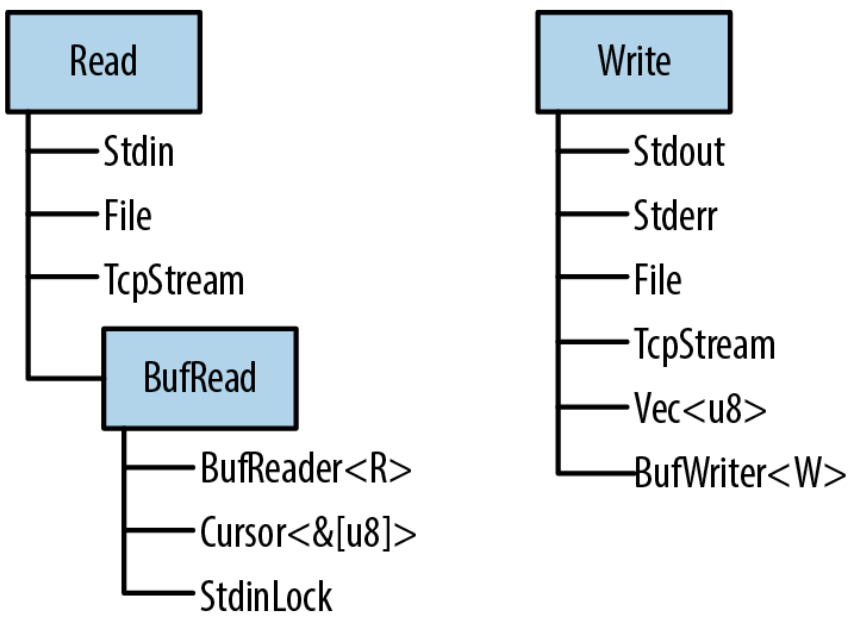
\includegraphics[width=0.8\textwidth]{../img/f18-1.png}
    \caption{Rust的三个主要的I/O trait以及一些实现了它们的类型}
    \label{f18-1}
\end{figure}

\section{Reader和Writer}

\emph{Reader}是你的程序可以从中读取字节的值。例如：
\begin{enumerate}
    \item 使用\texttt{std::fs::File::open(filename)}打开的文件
    \item 用于从网络中接收数据的\texttt{std::net::TcpStream}
    \item 进程用来读取标准输入的\texttt{std::io::stdin()}
    \item \texttt{std::io::Cursor<\&[u8]>}和\texttt{std::io::Cursor<Vec<u8>>}值，它们是从内存中的字节数组或vector中“读取”数据的reader
\end{enumerate}

\emph{Writer}是你的程序可以向其中写入字节的值。例如：
\begin{enumerate}
    \item 使用\texttt{std::fs::File::create(filename)}打开的文件
    \item 用于向网络中发送数据的\texttt{std::net::TcpStream}
    \item 用于写入到终端的\texttt{std::io::stdout()}和\texttt{std::io::stderr()}
    \item \texttt{Vec<u8>}，它也是一个writer，它的\texttt{write}方法把数据附加到尾部
    \item std::io::Cursor<Vec<u8>>，类似于上面，但允许你同时读取和写入数据，并可以在vector中定位到不同位置
    \item std::io::Cursor<\&mut [u8]>，和\texttt{std::io::Cursor<Vec<u8>>}很像，除了它不能让缓冲区增长，因为它只是已经存在的字节数组的切片
\end{enumerate}

因为有为reader和writer设计的标准trait（\texttt{std::io::Read}和\texttt{std::io::Write}），所以编写可以处理多种输入输出通道的泛型代码是非常普遍的。例如，这里有一个函数拷贝任意reader中的所有字节到任意writer：
\begin{minted}{Rust}
    use std::io::{self, Read, Write, ErrorKind};

    const DEFAULT_BUF_SIZE: usize = 8 * 1024;

    pub fn copy<R: ?Sized, W: ?Sized>(reader: &mut R, writer: &mut W)
        -> io::Result<u64>
        where R: Read, W: Write
    {
        let mut buf = [0; DEFAULT_BUF_SIZE];
        let mut written = 0;
        loop {
            let len = match reader.read(&mut buf) {
                Ok(0) => return Ok(written),
                Ok(len) => len,
                Err(ref e) if e.kind() == ErrorKind::Interrupted => continue,
                Err(e) => return Err(e),
            };
            writer.write_all(&buf[..len])?;
            written += len as u64;
        }
    }
\end{minted}

这是Rust的标准库中的\texttt{std::io::copy()}的实现。因为它是泛型的，你可以使用它从\texttt{File}中读取数据然后写入到\texttt{TcpStream}，或者从\texttt{Stdin}读取，然后写入到内存中的\texttt{Vec<u8>}，等等。

如果你看不明白这里的错误处理代码，请复习\hyperref[ch07]{第7章}。我们将在接下来的页面中一直使用\texttt{Result}类型；掌握它的工作原理很重要。

这三个\texttt{std::io}的trait：\texttt{Read}、\texttt{BufRead}、\texttt{Write}，以及\texttt{Seek}如此常用，以至于有一个只包含这些trait的\texttt{prelude}模块：
\begin{minted}{Rust}
    use std::io::prelude::*;
\end{minted}

本章中你还会见到它一到两次。我们通常也习惯于导入\texttt{std::io}模块自身：
\begin{minted}{Rust}
    use std::io::{self, Read, Write, ErrorKind};
\end{minted}

这里的\texttt{self}关键字声明了\texttt{io}作为\texttt{std::io}模块的一个别名。这样，\texttt{std::io::Result}和\texttt{std::io::Error}可以用\texttt{io::Result}和\texttt{io::Error}更精确地表示出来，等等。

\subsection{Reader}
\texttt{std::io::Read}有几个方法用于读取数据。所有这些方法都通过\texttt{mut}引用获取self参数。

\codeentry{reader.read(\&mut buffer)}
\hangparagraph{从数据源读取一些字节，并存储到给定的\texttt{buffer}中。\texttt{buffer}参数的类型是\texttt{\&mut [u8]}。它最多读取\texttt{buffer.len()}个字节。}
\hangparagraph{返回类型是\texttt{io::Result<u64>}，它是\texttt{Result<u64, io::Error>}的类型别名。当成功时，\texttt{u64}值是读取到的字节数——可能等于或着小于\texttt{buffer.len()}，\emph{即使还有更多的数据可以读取}。\texttt{Ok(0)}意味着没有更多的输入可以读取。}
\hangparagraph{当出错时，\texttt{.read()}返回\texttt{Err(err)}，其中\texttt{err}是一个\texttt{io::Error}值。\texttt{io::Error}是可打印的，为了便于阅读；对于程序来讲，它有一个\texttt{.kind()}方法返回一个\texttt{io::ErrorKind}类型的错误码。这个枚举的成员有例如\texttt{PermissionDenied}和\texttt{ConnectionReset}的名称。大多数的错误类型都不能被忽略，但有一种错误应该进行特殊处理。\texttt{io::ErrorKind::Interrupted}对应Unix的错误码\texttt{EINTR}，它意味着读取过程恰好被一个信号打断。除非你的程序想设计为根据信号做一些聪明的操作，否则它应该简单地重试读取操作。上一节中的\texttt{copy()}的代码，就是一个例子。}
\hangparagraph{如你所见，\texttt{.read()}方法非常底层，甚至直接继承了底层操作系统的怪癖。如果你要为一个新的数据源类型实现\texttt{Read} trait，这会赋予你极大的灵活性。但如果你尝试读取一些数据，就会非常难受。因此，Rust提供了几个更高级的便捷方法。它们都有基于\texttt{.read()}的默认实现。它们都处理了\texttt{ErrorKind::Interrupted}，因此你不需要再处理。}

\codeentry{reader.read\_to\_end(\&mut byte\_vec)}
\hangparagraph{读取reader种剩余的所有输入，将读到的数据附加到\texttt{byte\_vec}尾部，\texttt{byte\_vec}是一个\texttt{Vec<u8>}。返回一个\texttt{io::Result<uszie>}，表示读取到的字节数。}
\hangparagraph{这个方法读取的数据的大小没有限制，因此不要将它用于不受信任的源。（你可以使用\texttt{.take()}方法施加限制，如后文所述。}

\codeentry{reader.read\_to\_string(\&mut string)}
\hangparagraph{和上面相同，不过把数据附加到给定的\texttt{String}。如果流不是有效的UTF-8，它会返回一个\texttt{ErrorKind::InvalidData}错误。}
\hangparagraph{在一些编程语言中，字节输入和字符输入由不同的类型来处理。如今，UTF-8占据主导地位，Rust承认这一事实标准，并且完全支持UTF-8。其他字符集由开源的\texttt{encoding} crate提供支持。}

\codeentry{reader.read\_exact(\&mut buf)}
\hangparagraph{读取恰好足够的数据来填充给定的缓冲区。参数的类型是\texttt{\&mut [u8]}，如果在读取够\texttt{buf.len()}个字节之前reader的数据就已经耗光，那么它会返回一个\texttt{ErrorKind::UnexpectedEof}错误。}

上面这些是\texttt{Read} trait的主要方法。除此之外，还有三个以值获取\texttt{reader}的适配器方法，将它转换为一个迭代器或者一个不同的reader：

\codeentry{reader.bytes()}
\hangparagraph{返回一个输入流的字节的迭代器。item的类型是\texttt{io::Result<u8>}，因此每一个字节都需要进行错误检查。另外，它会逐字节调用\texttt{reader.read()}，因此如果reader没有缓存的话会非常低效。}

\codeentry{reader.chain(reader2)}
\hangparagraph{返回一个新的reader，首先产生\texttt{reader}的所有输入，然后产生\texttt{reader2}的所有输入。}

\codeentry{reader.take(n)}
\hangparagraph{返回一个新的reader，从和\texttt{reader}相同的数据源读取数据，但最多只读取\texttt{n}个字节。}

没有关闭reader的方法。reader和writer通常实现了\texttt{Drop}，因此它们会自动关闭。

\subsection{Buffered Reader}

\subsection{读取行}

\subsection{收集行}

\subsection{Writer}

\subsection{File}\label{file}
\chapter{并发}\label{ch19}
\chapter{异步编程}\label{ch20}

假设你正在编写一个聊天服务器。每个网络连接都有很多要解析的到来的包、要组装的发送的包、要管理的安全参数、要追踪的聊天组订阅等。同时为许多连接管理所有这些信息需要进行一些组织。

理想情况下，你可以简单地为每一个到来的连接启动一个单独的线程：
\begin{minted}{Rust}
    use std::{net, thread};

    let listener = net::TcpListener::bind(address)?;

    for socket_result in listener.incoming() {
        let socket = socket_result?;
        let groups = chat_group_table.clone();
        thread::spawn(|| {
            log_error(serve(socket, groups));
        });
    }
\end{minted}

这样对每一个连接都会创建一个新的线程运行\texttt{serve}函数，这个函数专门处理一个连接的需求。

这可以正常工作，直到一切都比计划的更加顺利很多，然后突然你就已经有了几万名用户。一个线程的栈增长到100KB或更多并不罕见，你可能不想就这样花费几GB的内存。要把任务分发到多个处理器上，线程是合适并且必须的，但它们的内存需求太大以至于我们通常需要一些补充的方式和线程一起使用，来减小资源占用。

你可以使用Rust的\emph{异步任务(asynchronous task)}来在单个线程或者线程池中交替执行很多独立的任务。异步任务类似于线程，但可以更快地创建、更高效地传递控制权、并且内存开销比线程少一个数量级。在单个程序中同时运行数十万个异步任务是完全可行的。当然，你的应用仍然可能被其他因素限制，例如网络带宽、数据库速度、计算、或者任务本身的内存需求，但使用异步任务的固有内存开销比使用线程的要小很多。

一般来讲，异步Rust代码看起来和普通的多线程代码非常相似，除了那些可能阻塞的操作，例如I/O或获取锁的处理有一点不同。特殊对待这些操作让Rust有更多的信息了解你的代码的行为，这为进一步优化提供了可能。上面代码的异步版本看起来像这样：
\begin{minted}{Rust}
    use async_std::{net, task};

    let listener = net::TcpListener::bind(address).await?;

    let mut new_connections = listener.incoming();
    while let Some(socket_result) = new_connections.next().await {
        let socket = socket_result?;
        let groups = chat_group_table.clone();
        task::spawn(async {
            log_error(serve(socket, groups).await);
        });
    }
\end{minted}

这里使用了\texttt{async\_std} crate的网络和任务模块，并在可能阻塞的调用后加上了\texttt{.await}。但整体的结构和基于线程的版本一样。

这一章的目标不止是帮你编写异步代码，还要向你展示它的工作细节，以便你可以预测它在你的应用中的表现，并了解它在哪些方面最有价值。

\begin{enumerate}
    \item 为了展示异步编程的机制，我们列出了涵盖所有核心概念的最小语言功能集：future、异步函数、\texttt{await}表达式、task、\texttt{block\_on}和\texttt{spawn\_local} executor。
    \item 然后我们会展示异步块和\texttt{spawn} executor。它们是完成真实工作的最基础的部分，但从概念上讲，它们只是我们刚才提到过的功能的变体。在这个过程中，我们会指出一些你可能会遇到的异步编程特有的问题并解释如何处理它们。
    \item 为了展示所有功能的协调工作，我们会展示一个聊天服务器和客户端的完整代码，上面的代码片段就是其中一部分。
    \item 为了演示原语future和executor如何工作，我们会展示\texttt{spawn\_blocking}和\texttt{block\_on}的简单实现。
    \item 最后，我们介绍了异步接口中经常出现的\texttt{Pin}类型，它被用来确保异步函数和块future被安全地使用。
\end{enumerate}

\section{从同步到异步}

考虑当你调用下面的（不是异步的）函数时会发生什么：
\begin{minted}{Rust}
    use std::io::prelude::*;
    use std::net;

    fn cheapo_request(host: &str, port: u16, path: &str)
                          -> std::io::Result<String>
    {
        let mut socket = net::TcpStream::connect((host, port))?;

        let request = format!("GET {} HTTP/1.1\r\nHost: {}\r\n\r\n", path, host);
        socket.write_all(request.as_bytes())?;
        socket.shutdown(net::Shutdown::Write)?;

        let mut response = String::new();
        socket.read_to_string(&mut response)?;

        Ok(response)
    }
\end{minted}

这会打开一个到web服务器的TCP连接，以过时的协议向它发送一个简单的HTTP请求，\footnote{如果你真的需要一个HTTP客户端，考虑使用一些非常优秀的crate例如\texttt{surf}或\texttt{reqwest}，它们会正确并且异步地完成任务。这个客户端基本只是设法获得HTTPS重定向。}然后读取响应。\autoref{f20-1}展示了这个函数的执行过程随时间的变化。

\begin{figure}[htbp]
    \centering
    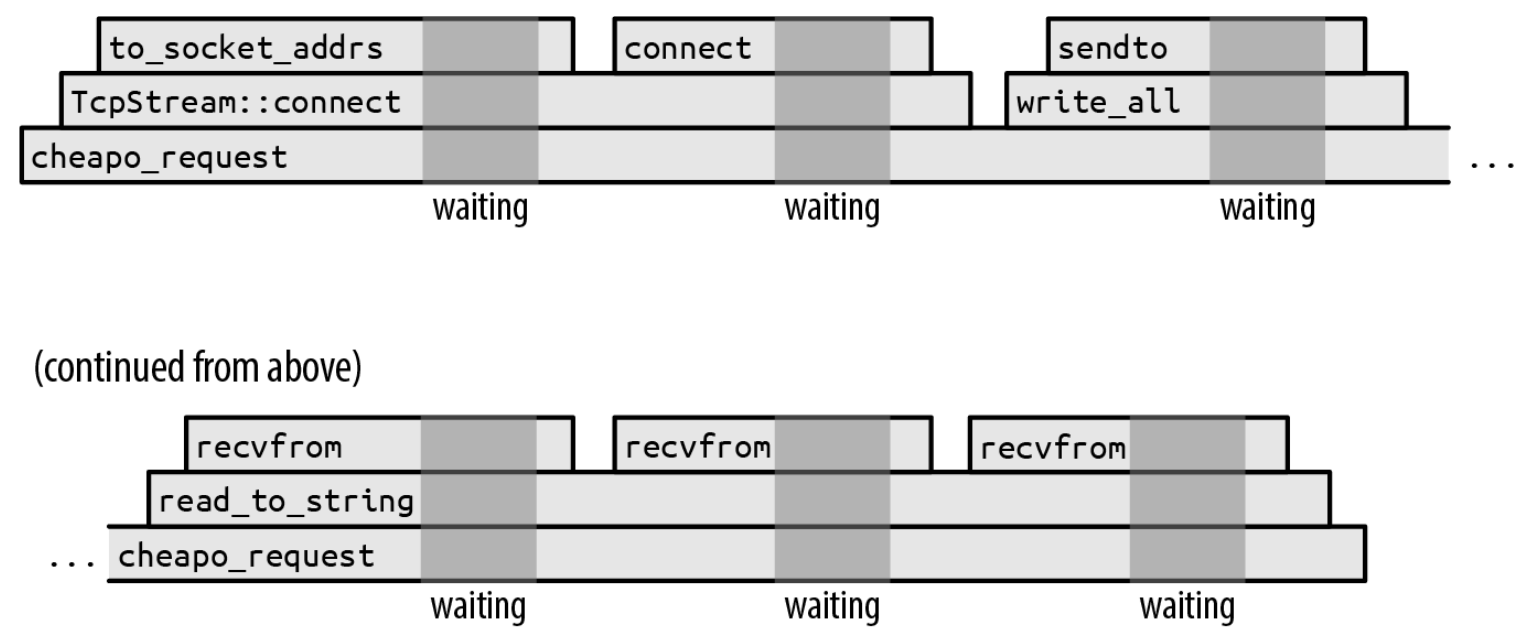
\includegraphics[width=0.8\textwidth]{../img/f20-1.png}
    \caption{一个同步HTTP请求的过程（深颜色的区域标识等待操作系统）}
    \label{f20-1}
\end{figure}

图中展示了从左到右随着时间的推移，函数的调用栈的变化。每一个函数调用都是一个方块，位于它的调用者上面。显然，\texttt{cheapo\_request}函数贯穿整个执行过程。它调用了Rust标准库里的函数例如\texttt{TcpStream::connect}和\texttt{TcpStream}的\texttt{write\_all}和\texttt{read\_to\_string}实现。这些对其他函数的调用依次进行，但最终程序会进行\emph{系统调用}，请求操作系统完成真正的工作，例如打开TCP连接，或者读写一些数据。

深灰色的区域表示程序正在等待操作系统完成系统调用。我们并没有按比例绘制这些时间。因为加入我们按比例绘制，整个图都将是深灰色：在实践中，这个函数把几乎所有时间都用在等待操作系统上。上面代码的执行时间将是系统调用之间的窄条。

当函数等待系统调用返回时，它所在的线程会阻塞住：它不能做任何事，直到系统调用结束。一个线程的栈达到几百或几千字节并不罕见，因此如果这是一个更大的系统的一部分，并且有很多线程做类似的任务，锁住这些线程的资源但除了等待什么也不做的代价是非常昂贵的。

为了解决这个问题，一个线程需要能在等待系统调用完成的同时去执行其他的任务。但如何实现这一点并不明显。例如，我们用来从套接字读取响应的函数的签名是：
\begin{minted}{Rust}
    fn read_to_string(&mut self, buf: &mut String) -> std::io::Result<usize>;
\end{minted}

它的类型表明了：这个函数直到工作完成或者出错时才会返回。这个函数是\emph{同步的}：当操作完成时调用者才恢复。如果我们想在操作系统进行工作的同时用我们的线程去做别的任务，那么我们需要一个新的提供这个函数的\emph{异步}版本的I/O库。

\subsection{\texttt{Future}}
Rust支持异步操作的方法是引入一个trait：\texttt{std::future::Future}：
\begin{minted}{Rust}
    trait Future {
        type Output;
        // 现在，把`Pin<&mut Self>`看作`&mut Self`就好了。
        fn poll(self: Pin<&mut Self>, cx: &mut Context<'_>) -> Poll<Self::Output>;
    }

    enum Poll<T> {
        Ready(T),
        Pending,
    }
\end{minted}

一个\texttt{Future}代表一个可以测试是否完成的操作。一个future的\texttt{poll}方法从来不会等待操作完成：它总是立即返回。如果操作完成了，\texttt{poll}会返回\texttt{Poll::Ready(output)}，其中\texttt{output}是最后的结果。否则，它会返回\texttt{Pending}。当且仅当future值得再次poll时，它会通过调用一个\emph{waker}来通知我们，这是一个由\texttt{Context}提供的回调函数。我们称之为异步编程的“piñata 模型” ：你唯一能对future做的就是使用\texttt{poll}敲打它，直到有一个值掉出来。

所有现代的操作系统都包含一些系统调用的变体，我们可以用它们来实现这种poll接口。例如在Unix和Windows上，如果你把网络套接字设置为非阻塞模式，那么如果它们正在阻塞时进行read和write会返回错误，你必须稍后再试。

因此\texttt{read\_to\_string}的一个异步版本的签名大概是这样：
\begin{minted}{Rust}
    fn read_to_string(&mut self, buf: &mut String)
        -> impl Future<Output = Result<usize>;
\end{minted}

除了返回类型之外，这和我们之前展示的签名一样：异步的版本返回\emph{一个\texttt{Result<usize>}的future}。你需要poll这个future，直到从它得到一个\texttt{Ready(result)}。每次它被poll时，都会尽可能地继续读取。最后的\texttt{result}给你成功的值或者错误的值，就像普通的I/O操作一样。这是通常的模式：异步版本的任何函数和同步版本的函数获取相同的参数，但返回类型有一个\texttt{Future}包装。

调用这个版本的\texttt{read\_to\_string}并不会真的读取任何内容；它所有的任务就是构造并返回一个future，这个future会在被poll时进行真正的工作。这个future必须包含处理请求所需的所有信息。例如，这个\texttt{read\_to\_string}返回的future必须记住调用它的输入流，和它需要写入数据的\texttt{String}。事实上，因为这个future持有了\texttt{self}和\texttt{buf}的引用，因此这个\texttt{read\_to\_string}的真正的签名必须是：
\begin{minted}{Rust}
    fn read_to_string<'a>(&'a mut self, buf: &'a mut String)
        -> impl Future<Output = Result<usize>> + 'a;
\end{minted}

这个附加的生命周期指示了返回的future和它借用的\texttt{self}和\texttt{buf}的生命周期一样长。

\texttt{async-std} crate提供了\texttt{std}的所有I/O设施的异步版本，包括一个有\texttt{read\_to\_string}方法的异步\texttt{Read} trait。\texttt{async-std}密切地遵循了\texttt{std}的设计，尽可能地在自己的接口中重用\texttt{std}的类型，因此这两个世界中的错误、结果、网络地址、和其他大多数相关的数据都是兼容的。熟悉\texttt{std}有助于使用\texttt{async-std}，反之亦然。

\texttt{Future} trait的一个规则是，一旦一个future返回了\texttt{Poll::Ready}，它会假设它决不会再次被poll。一些future在自己被overpoll时简单地永远返回\texttt{Poll::Pending}；其它的可能panic或者挂起。（它们绝不能违反内存或线程安全性，或者导致未定义行为）\texttt{Future} trait的\texttt{fuse}适配器将任何future转换成overpoll时永远返回\texttt{Poll::Pending}。但通常消费future的方法都遵循这个规则，因此\texttt{fuse}通常不是必须的。

如果poll听起来效率底下，请不必担心。Rust的异步架构是精心设计的，所以只要你的基本I/O函数例如\texttt{read\_to\_string}是正确实现的，那么你只会在值的时poll一个future。每一次\texttt{poll}被调用时，某个东西应该返回\texttt{Ready}，或者至少向目标前进一步。我们将在“\nameref{WhenPoll}”中解释这是如何工作的。

但使用future看起来有一个挑战：当你poll时，如果你得到了\texttt{Poll::Pending}那你应该怎么做？你将不得不四处寻找这个线程暂时可以做的其他工作，并记住一段时间之后返回到这个future，然后再次poll。你的整个系统将因为持续追踪谁正在pending和当它们完成时应该做什么而变得杂乱无章。我们的\texttt{cheapo\_request}函数的简洁性会被破坏。

好消息是：它并不是这样的！

\subsection{\texttt{async}函数和\texttt{await}表达式}
这里有一个\emph{异步函数}版本的\texttt{cheapo\_request}：
\begin{minted}{Rust}
    use async_std::io::prelude::*;
    use async_std::net;

    async fn cheapo_request(host: &str, port: u16, path: &str)
                                -> std::io::Result<String>
    {
        let mut socket = net::TcpStream::connect((host, port)).await?;

        let request = format!("GET {} HTTP/1.1\r\nHost: {}\r\n\r\n", path, host);
        socket.write_all(request.as_bytes()).await?;
        socket.shutdown(net::Shutdown::Write)?;

        let mut response = String::new();
        socket.read_to_string(&mut response).await?;

        Ok(response)
    }
\end{minted}

这和之前的版本基本相同，除了：
\begin{enumerate}
    \item 函数以\texttt{async}代替\texttt{fn}开头。
    \item 它使用了\texttt{async\_std} crate里的异步版本的\texttt{TcpStream::connect, write\_all, read\_to\_string}。它们都返回结果的future（本节中的示例使用了\texttt{async\_std}的1.7版本）。
    \item 每一次调用返回future的函数之后，代码都会加上\texttt{.await}。尽管这看起来像是访问一个结构体的\texttt{await}字段，但它实际上是语言内置的一个特殊语法，它会等待一个future直到它准备好。\texttt{await}表达式会求出future的最终值。这个函数正是通过它获取\texttt{connect, write\_all, read\_to\_string}的结果。
\end{enumerate}

和普通的函数不同，当你调用异步函数时，它会在执行实际的主体代码之前立即返回。显然，调用的返回值还没有被计算出来；你得到的是它的最终值的\emph{future}。因此如果你执行这行代码：
\begin{minted}{Rust}
    let response = cheapo_request(host, port, path);
\end{minted}

那么\texttt{response}将是一个\texttt{std::io::Result<String>}的future，\texttt{cheapo\_request}的函数体还没有开始执行。你不需要调整异步函数的返回类型；Rust会自动把\texttt{async fn f(...) -> T}看做一个返回\texttt{T}的future而不是直接返回\texttt{T}的函数。

一个异步函数返回的future包含了函数体运行时所需的所有信息：函数的参数、局部变量所需的空间，等等。（就好像你把调用栈捕获为了一个普通的Rust值。）因此\texttt{response}必须包含传入的\texttt{host, port, path}，因为\texttt{cheapo\_request}的函数体需要它们才能运行。

future的具体类型由编译器根据函数体和参数自动生成。这个类型并没有名称；你只知道它实现了\texttt{Future<Output=R>}，其中\texttt{R}是异步函数的返回类型。从这一点来看，异步函数的future类似于闭包：闭包也有匿名类型、也是由编译器生成并且实现了\texttt{FnOnce}、\texttt{Fn}和\texttt{FnMut} trait。

当你第一次poll \texttt{cheapo\_request}返回的future时，将会从函数体的尾部开始运行到第一个由\texttt{TcpStream::connect}返回的future的\texttt{await}。这个\texttt{await}表达式会poll \texttt{connect} future，如果它还没准备好，那么它会向调用者返回\texttt{Poll::Pending}：直到\texttt{TcpStream::connect}的future返回\texttt{Poll::Ready}时，对\texttt{cheapo\_request}的future的poll才能继续通过第一个\texttt{await}。因此表达式\texttt{TcpStream::connect(...).await}的一个大概等价的写法是：
\begin{minted}{Rust}
    {
        // 注意：这是伪代码，不是有效的Rust代码
        let connect_future = TcpStream::connect(...);
        'retry_point:
        match connect_future.poll(cx) {
            Poll::Ready(value) => value,
            Poll::Pending => {
                // 设置`cheapo_request`的future的下一次`poll`
                // 从'retry_point处恢复执行。
                ...
                return Poll::Pending
            }
        }
    }
\end{minted}

一个\texttt{await}表达式会获取future的所有权然后poll它。如果它已经准备好，那么future的最终值就是\texttt{await}表达式的值，并且会继续往下执行。否则，它向调用者返回\texttt{Poll::Pending}。

但关键的是，下一次poll \texttt{cheapo\_request}的future时将不会再次从函数的首部开始：相反，它从poll \texttt{connect\_future}的地方开始\emph{恢复(resume)}执行。直到future准备好之后我们才会继续执行这个异步函数的其他部分。

随着\texttt{cheapo\_request}的future继续被poll，它会从函数体里的一个\texttt{await}开始执行到下一个，只有当它正在等待的子future ready时才会继续。因此，\texttt{cheapo\_request}的future将会被poll多少次取决于子future的行为和函数本身的控制流。\texttt{cheapo\_request}的future会追踪下一次\texttt{poll}时的恢复点和所有的局部状态——变量、参数、临时值——恢复需要这些。

在函数中间挂起并稍后恢复执行的能力是异步函数独有的。当普通函数返回时，它的栈帧就消失了。因为\texttt{await}表达式依赖于恢复执行的能力，所以你只能在异步函数里使用它们。

在撰写本书时，Rust还不允许trait有异步方法。只有自由函数和特定类型固有的方法才可以是异步的。取消这个限制需要对语言进行一些修改。与此同时，如果你需要定义包含异步函数的trait，可以考虑使用\texttt{async-trait} crate，它提供了一个基于宏的解决方案。

\subsection{在同步代码中调用异步函数：\texttt{block\_on}}
某种意义上讲，异步函数只是在推卸责任。在异步函数里很容易获取一个future的值：只需要\texttt{await}它。但异步函数\emph{本身}也返回一个future，因此现在调用者需要负责poll它。最后，总有一个地方必须实际等待一个值。

我们可以使用\texttt{async\_std}的\texttt{task::block\_on}函数在普通的同步函数（例如\texttt{main}）中调用\texttt{cheapo\_request}，它获取一个future并且poll它直到它产生一个值：
\begin{minted}{Rust}
    fn main() -> std::io::Result<()> {
        use async_std::task;

        let response = task::block_on(cheapo_request("example.com", 80, "/))?;
        println!("{}", response);
        Ok(())
    }
\end{minted}

因为\texttt{block\_on}是一个产生异步函数的最终值的同步函数，你可以将它看作是异步世界到同步世界的适配器。但它阻塞的特性也意味着你永远不应该在一个异步函数里使用\texttt{block\_on}：它会阻塞整个线程直到值准备好。作为代替，请使用\texttt{await}。

\autoref{f20-2}展示了\texttt{main}的一个可能的执行过程。

\begin{figure}[htbp]
    \centering
    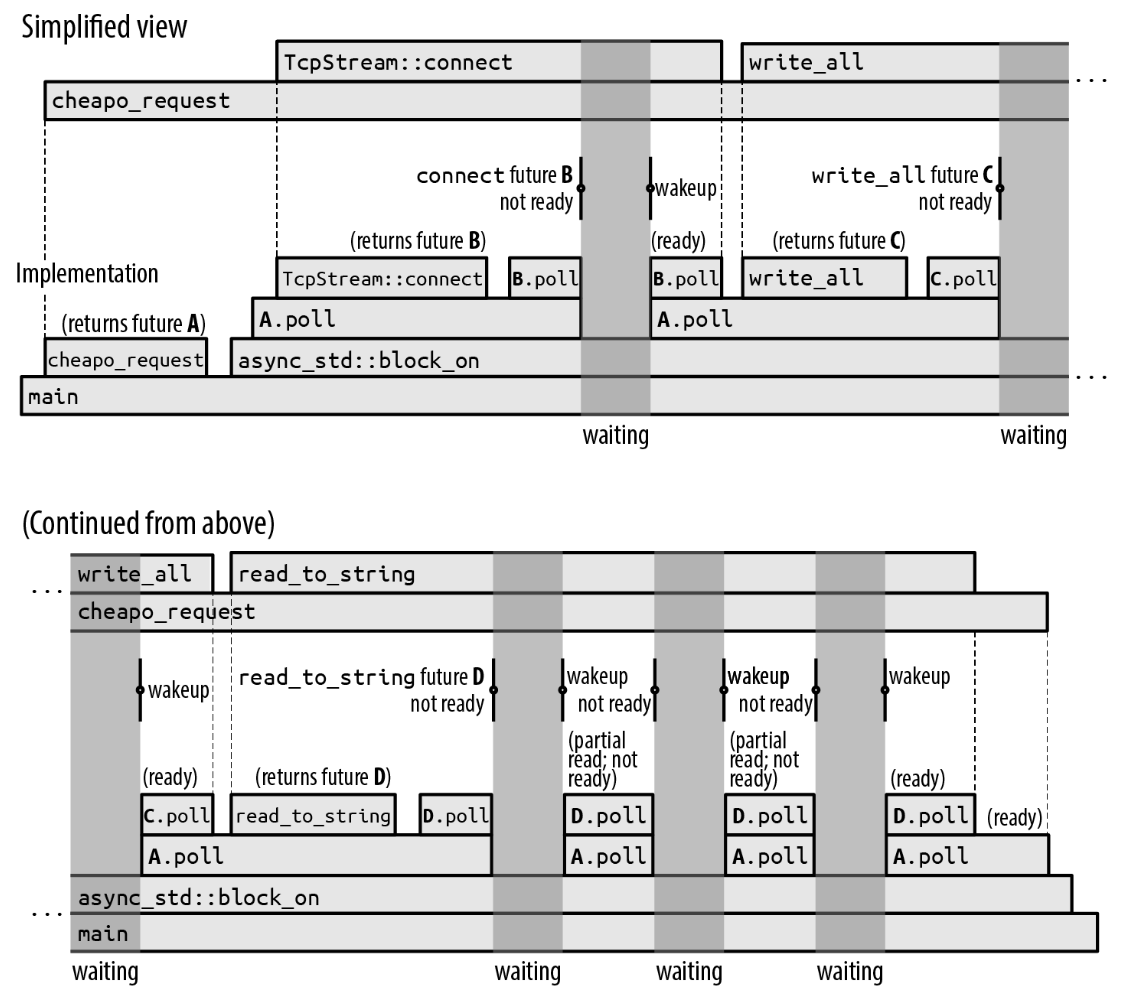
\includegraphics[width=0.9\textwidth]{../img/f20-2.png}
    \caption{阻塞等待一个异步函数}
    \label{f20-2}
\end{figure}

上面的时间线，“简化视图”，展示了程序的异步调用的抽象视图：\texttt{cheapo\_request}首先调用了\texttt{TcpStream::connect}来获取一个套接字，然后对套接字调用了\texttt{write\_all}和\texttt{read\_to\_string}。然后它返回。这和本章前面的同步版本的\texttt{cheapo\_request}的时间线非常相似。

但这里每一个异步调用都是多阶段的过程：一个future被创建，然后被poll直到它准备好，可能还会创建并poll其他子future。下面的时间线，“实现”，展示了实现了这个异步行为的实际同步调用。这是一个介绍普通的异步执行过程中到底发生了什么的好机会：
\begin{enumerate}
    \item 首先，\texttt{main}调用\texttt{cheapo\_request}，它返回最终结果的future \texttt{A}。然后\texttt{main}把这个future传给了\texttt{async\_std::block\_on}，它会poll \texttt{A}。
    \item poll future \texttt{A}允许\texttt{cheapo\_request}的函数体开始执行。函数里调用了\texttt{TcpStream::connect}来获取一个套接字的future \texttt{B}并await它。更确切地说，因为\texttt{TcpStream::connect}可能会遇到错误，因此\texttt{B}是一个\texttt{Result<TcpStream, std::io::Error}的future。
    \item future \texttt{B}被\texttt{await} poll。因为网络连接还没有建立好，所以\texttt{B.poll}返回\texttt{Poll::Pending}，但会设置好当套接字准备好后唤醒调用它的任务。
    \item 因为future \texttt{B}还没有准备好，\texttt{A.poll}也会向它的调用者\texttt{block\_on}返回\texttt{Poll::Pending}。
    \item 因为\texttt{block\_on}没有别的事情可做，它会陷入睡眠。这时整个线程会阻塞。
    \item 当\texttt{B}的连接准备好之后，它会唤醒poll它的任务。这促使\texttt{block\_on}开始行动，它会尝试再次poll future \texttt{A}。
    \item poll \texttt{A}促使\texttt{cheapo\_request}在它的第一个\texttt{await}处恢复执行，然后再次poll \texttt{B}。
    \item 这一次，\texttt{B}准备好了：套接字已经创建完毕，因此它返回\texttt{Poll::Ready(Ok(socket))}到\texttt{A.poll}。
    \item 到此\texttt{TcpStream::connect}的异步调用就完成了。\texttt{TcpStream::connect(...).await}表达式的值就是\texttt{Ok(socket)}。
    \item \texttt{cheapo\_request}的函数体会继续正常执行，使用\texttt{format!}宏构造请求字符串并传递给\texttt{socket.write\_all}。
    \item 因为\texttt{socket.write\_all}是一个异步函数，它会返回一个future \texttt{C}，\texttt{cheapo\_request}会await \texttt{C}。
\end{enumerate}

剩余的流程和之前相似。在\autoref{f20-2}所示的执行流程中，\texttt{socket.read\_to\_string}在准备好之前被poll了四次，每一次都会从套接字读取\emph{一些}数据，但\texttt{read\_to\_string}被指定为一直读取到输入的末尾，这需要好几次的操作。

听起来编写一个一直调用\texttt{poll}的循环并不难。但让\texttt{async\_std::task::block\_on}真正有价值的是：它知道怎么睡眠到恰好future值得再次poll，而不是浪费处理器的时间和电量来进行几十亿次无用的\texttt{poll}调用。基本的I/O函数例如\texttt{connect}和\texttt{read\_to\_string}返回的future保留了传递给\texttt{poll}的\texttt{Context}参数提供的唤醒器，并在\texttt{block\_on}应该醒来并再次尝试poll时调用唤醒器。我们将在“\nameref{WhenPoll}”中通过实现一个简单版本的\texttt{block\_on}来展示这具体是怎么工作的。

和我们之前展示的原始的同步版本一样，这个异步版本的\texttt{cheapo\_request}方法也把几乎所有的时间花费在等待操作完成上。如果时间轴是按比例绘制的，那么图将几乎完全是深灰色的，只有当程序被唤醒时会有几个计算过程对应的很细的条。

这里讲了很多细节。幸运的是，你通常可以只考虑简化的上层时间线：一些函数调用是同步的，其他是异步的并需要一个\texttt{await}，但它们都只是函数调用。Rust的异步支持的成功取决于帮助程序员在实践中只需要考虑简化的视图，不会被实现的来回跳转干扰。

\subsection{spawn异步任务}
\texttt{async\_std::task::block\_on}函数会阻塞直到一个future的值准备好。但在单个future上完全阻塞一个线程并不比同步调用更好：本章的目的是让线程在等待的同时\emph{做别的工作}。

为了实现这一点，你可以使用\texttt{async\_std::task::spawn\_local}。这个函数接受一个future并把它添加到一个池，当\texttt{block\_on}阻塞等待的future还没准备好时\texttt{block\_on}会poll这个池。因此如果你把一堆future传递给\texttt{spawn\_local}并且之后对最终结果的future调用\texttt{block\_on}，\texttt{block\_on}会poll每一个被spawn的future（当它们可以进一步执行时），并发运行整个池，直到结果准备好。

在撰写本书时，只有当你启用\texttt{async-std} crate的\texttt{unstable}特性时\texttt{spawn\_local}才可用。你需要在\emph{Cargo.toml}中用这样的一行引入\texttt{async-std}：
\begin{minted}{toml}
    async-std = { version = "1", features = ["unstable"] }
\end{minted}

\texttt{spawn\_local}函数是标准中用于启动新线程的\texttt{std::thread::spawn}函数的异步版本的类似物：
\begin{enumerate}
    \item \texttt{std::thread::spawn(c)}接收闭包\texttt{c}然后启动一个线程运行它，返回一个\texttt{std::thread::JoinHandle}，它的\texttt{join}方法会等待线程结束并返回\texttt{c}返回的内容。
    \item \texttt{async\_std::task::spawn\_local(f)}接收future \texttt{f}并把它添加到当前线程调用\texttt{block\_on}时会poll的池里。\texttt{spawn\_local}会返回它自己的\texttt{async\_std::task::JoinHandle}类型，它本身是一个future，你可以await它来获取\texttt{f}的最终值。
\end{enumerate}

例如，假设我们想让一个HTTP请求的集合并发执行。这是第一次尝试：
\begin{minted}{Rust}
    pub async fn many_requests(requests: Vec<(String, u16, String)>)
                               -> Vec<std::io::Result<String>>
    {
        use async_std::task;

        let mut handles = vec![];
        for (host, port, path) in requests {
            handles.push(task::spawn_local(cheapo_request(&host, port, &path)));
        }

        let mut results = vec![];
        for handle in handles {
            results.push(handle.await);
        }

        results
    }
\end{minted}

这个函数对\texttt{requests}的每个元素调用\texttt{cheapo\_request}，将每一个调用返回的future传给\texttt{spawn\_local}。它把最后的\texttt{JoinHandle}收集到一个vector并且await每一个。以任意顺序await join handles都是没问题的：因为请求已经被spawn，它们的future将会被按需poll，即这个线程调用了\texttt{block\_on}并且无事可做时。所有的请求会并发运行。一旦它们完成，\texttt{many\_requests}会向调用者返回结果。

上面的代码几乎是正确的，但Rust的借用检查器担心\texttt{cheapo\_request}的future的生命周期：
\begin{minted}{text}
    error: `host` does not live long enough
        handles.push(task::spawn_local(cheapo_request(&host, port, &path)));
                                       ---------------^^^^^-------------
                                       |              |
                                       |              borrowed value does not
                                       |              live long enough
                         argument requires that `host` is borrowed for `'static`
    }
    - `host` dropped here while still borrowed
\end{minted}

\texttt{path}也有一个类似的错误。

自然地，如果我们向异步函数传递引用，那么它们返回的future就必须持有这些引用，因此出于安全性future不能比它们借用的值生存的更久。任何持有引用的其他值也有相同的限制。

问题在于\texttt{spawn\_local}不能确保你会在\texttt{host}和\texttt{path}被drop之前等待任务结束。事实上，\texttt{spawn\_local}只接受生命周期是\texttt{'static}的future，因为你可以简单地忽略它返回的\texttt{JoinHandle}并让任务在程序的剩余部分执行时继续运行。这并不是异步任务独有的问题：当你尝试用\texttt{std::thread::spawn}启动一个线程，并且它的闭包捕获了局部变量的引用时也会遇到类似的错误。

一种解决这个问题的方法是创建另一个版本的获取参数所有权的异步函数：
\begin{minted}{Rust}
    async fn cheapo_owning_request(host: String, port: u16, path: String)
                                   -> std::io::Result<String> {
        cheapo_request(&host, port, &path).await
    }
\end{minted}

这个函数接收\texttt{String}而不是\texttt{\&str}引用，因此它的future自身将拥有\texttt{host}和\texttt{path}，并且生命周期是\texttt{'static}。借用检查器可以看到它立刻await了\texttt{cheapo\_request}的future，并且因此如果这个future被poll，它借用的\texttt{host}和\texttt{path}变量肯定还在。一切都没有问题。

使用\texttt{cheapo\_owning\_request}，你可以像这样spwan所有的请求：
\begin{minted}{Rust}
    for (host, port, path) in requests {
        handles.push(task::spawn_local(cheapo_owning_request(host, port, path)));
    }
\end{minted}

你可以使用\texttt{block\_on}在同步的\texttt{main}函数中调用\texttt{many\_requests}：
\begin{minted}{Rust}
    let requests = vec![
        ("example.com".to_string(),      80, "/".to_string()),
        ("www.red-bean.com".to_string(), 80, "/".to_string()),
        ("en.wikipedia.org".to_string(), 80, "/".to_string()),
    ];

    let results = async_std::task::block_on(many_requests(requests));
    for result in results {
        match result {
            Ok(response) => println!("{}", response),
            Err(err) => eprintln!("error: {}", err),
        }
    }
\end{minted}

这段代码会在\texttt{block\_on}的调用中并发运行三个请求。每个请求会在当其他的请求阻塞时抓住几乎继续执行，它们全部在调用者线程中执行。\autoref{f20-3}中展示了三个\texttt{cheapo\_request}调用的可能的执行过程。

\begin{figure}[htbp]
    \centering
    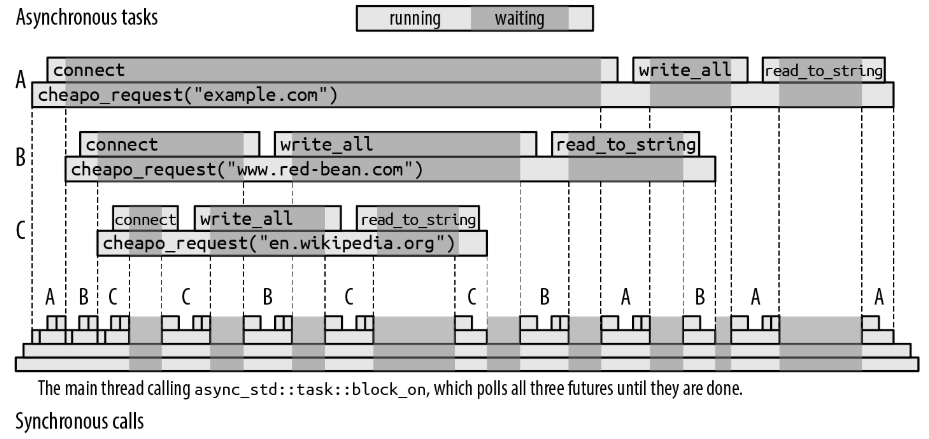
\includegraphics[width=0.9\textwidth]{../img/f20-3.png}
    \caption{在单个线程中运行三个异步任务}
    \label{f20-3}
\end{figure}

（我们鼓励你自己尝试运行这段代码，使用\texttt{eprintln!}在\texttt{cheapo\_request}首部和每一个\texttt{await}表达式之后打印消息，这样你可以看到这些调用如何交错执行。）

对\texttt{many\_requests}的调用（为了简单没有展示）spawn了三个异步的任务，分别用\texttt{A}、\texttt{B}、\texttt{C}标记。\texttt{block\_on}开始时先poll \texttt{A}，\texttt{A}会开始连接到\texttt{example.com}。这会立刻返回\texttt{Poll::Pending}，\texttt{block\_on}会把注意移动到下一个spawn的任务，然后poll future \texttt{B}，最后是\texttt{C}，它们会开始连接各自的服务器。

当所有可以poll的future都返回了\texttt{Poll::Pending}之后，\texttt{block\_on}会进入睡眠，直到其中一个\texttt{TcpStream::connect} future指示它的任务值得再次poll。

在这次执行中，服务器\texttt{en.wikipedia.org}比其他的响应得更快，因此这个任务最先完成。当一个spawn的任务完成时，它会把值保存在\texttt{JoinHandle}并标记它已经准备好了，这样\texttt{many\_requests} await它时无需等待，可以继续执行。最后，其它的\texttt{cheapo\_request}要么成功要么返回错误，然后\texttt{many\_request}本身可以返回了。最后，\texttt{main}接收\texttt{block\_on}返回的结果的vector。

所有这些执行都发生在单个线程中，三个\texttt{cheapo\_request}的调用通过对future的poll实现交错执行。一个异步调用看起来像是一个运行到完成的单个函数调用，但实际上异步调用由一系列对future的\texttt{poll}方法的同步调用实现。每一个单独的\texttt{poll}调用都可以快速返回，让出线程从而让其他异步调用可以执行。

我们终于达成了我们在本章开头设置的目标：让一个线程在等待I/O完成的同时去执行其他的工作，这样线程的资源不会因等待而浪费。更妙的是，达成这个目标的代码看起来非常像普通的Rust代码：一些函数被标记为\texttt{async}、一些函数调用后面有\texttt{.await}、使用的函数来自\texttt{async\_std}而不是\texttt{std}，但除此之外，它就是普通的Rust代码。

异步任务和线程有一个不同之处需要牢记：异步任务只有在\texttt{await}表达式处被await的future返回\texttt{Poll::Pending}时才会切换到另一个异步任务。这意味着如果你在\texttt{cheapo\_request}中放了一段长时间运行的计算代码，那么在它完成之前，任何传给\texttt{spawn\_local}的其他任务都没有机会运行。而使用线程时没有这个问题：操作系统可以在任何地方挂起任何线程并设置计时器来确保没有线程可以垄断处理器。

异步代码依赖于共享线程的future的协作。如果你需要让长时间计算和异步代码共存，本章后面的“\nameref{LongCompute}”中介绍了一些方法。

\subsection{\texttt{async}块}
除了异步函数之外，Rust还支持\emph{异步块(asynchronous block)}。与一个普通的快块返回最后一个表达式的值不同，一个异步块返回最后一个表达式的\emph{值的future}。你可以在异步块里使用\texttt{await}表达式。

异步块看起来就像普通的块表达式，在前边加上\texttt{async}关键字：
\begin{minted}{Rust}
    let serve_one = async {
        use async_std::net;

        // 监听连接并接受
        let listener = net::TcpListener::bind("localhost:8087").await?;
        let (mut socket, _add) = listener.accept().await?;

        // 通过`socket`与客户端交互
        ...
    };
\end{minted}

这里用一个future初始化了\texttt{serve\_one}，当poll它时，它会监听并处理单个TCP连接。块的代码直到\texttt{serve\_one}被poll才会执行，就像异步函数只有在它的future被poll时才会执行一样。

如果你在异步块里使用了\texttt{?}操作符，它会从块里返回，而不是从所处的函数返回。例如，如果上面的\texttt{bind}调用返回一个错误，那么\texttt{?}操作符会返回它作为\texttt{serve\_one}的最终值。类似的，\texttt{return}表达式会从异步块里返回，而不是从外层的函数返回。

如果一个异步块引用了周围代码里的变量，它的future会捕获那些变量，就像闭包一样。并且和\texttt{move}闭包一样（见“\nameref{StealClosure}”），你可以以\texttt{async move}来创建获取变量所有权的块，而不是持有变量的引用。

异步块提供了一种精确的分离出想要异步运行的部分代码的方法。例如，在上一节中，\texttt{spawn\_local}需要\texttt{'static} future，因此我们定义了\texttt{cheapo\_owning\_request}包装函数来得到一个获取参数所有权的future。你可以简单地在一个异步块里调用\texttt{cheapo\_request}而不需要分离出包装函数来实现相同的效果：
\begin{minted}{Rust}
    pub async fn many_requests(requests: Vec<(String, u16, String)>)
                               -> Vec<std::io::Result<String>>
    {
        use async_std::task;

        let mut handles = vec![];
        for (host, port, path) in requests {
            handles.push(task::spawn_local(async move {
                cheapo_request(&host, port, &path).await
            }));
        }
        ...
    }
\end{minted}

因为这是一个\texttt{async move}块，所以它的future获取了\texttt{String}值\texttt{host}和\texttt{path}的所有权，就类似\texttt{move}闭包一样。然后它向\texttt{cheapo\_request}传递引用，借用检查器可以看到块的\texttt{await}表达式获取了\texttt{cheapo\_request}的future的所有权，因此\texttt{host}和\texttt{path}的引用不可能比它们借用的被捕获的变量生存的更久。异步块和\texttt{cheapo\_owning\_request}完成了同样的事，但所需的样板代码更少。

一个你可能遇到的问题是没有语法能指定异步块的返回类型，即异步函数参数后跟的\texttt{-> T}。当使用\texttt{?}操作符时这可能会导致问题：
\begin{minted}{Rust}
    let input = async_std::io::stdin();
    let future = async {
        let mut line = String::new();

        // 这会返回`std::io::Result<usize>`。
        input.read_line(&mut line).await?;

        println!("Read line: {}", line);

        Ok(())
    };
\end{minted}

这会因为如下错误失败：
\begin{minted}{text}
    error: type annotations needed
       |
    42 |     let future = async {
       |         ------ consider giving `future` a type
    ...
    46 |         input.read_line(&mut line).await?;
       |         ^^^^^^^^^^^^^^^^^^^^^^^^^^^^^^^^^ cannot infer type
\end{minted}

Rust不能分辨异步块的返回类型应该是什么。\texttt{read\_line}方法返回\texttt{Result<(), std::io::Error>}，但因为\texttt{?}操作符使用了\texttt{From} trait来在需要时转换成指定的错误类型，所以这个异步块的返回类型是\texttt{Result<(), E>}，其中\texttt{E}可能是任何实现了\texttt{From<std::io::Error>}的类型。

Rust未来的版本可能会添加指定\texttt{async}块的返回类型的语法。但现在，可以通过手动写出最后的\texttt{Ok}的类型来解决这个问题：
\begin{minted}{Rust}
    let future = async {
        ...
        Ok::<(), std::io::Error>(())
    };
\end{minted}

因为\texttt{Result}是一个需要成功和错误类型作为参数的泛型类型，我们可以像这里一样使用\texttt{Ok}或\texttt{Err}指定那些类型参数。

\subsection{从异步块中构建异步函数}
异步块给了我们另一种实现和异步函数相同效果的方法，并且更加灵活一点。例如，我们可以将我们的\texttt{cheapo\_request}写成一个普通的、同步的返回异步块的future的函数：
\begin{minted}{Rust}
    use std::io;
    use std::future::Future;

    fn cheapo_request<'a>(host: &'a str, port: u16, path: &'a str)
        -> impl Future<Output = io::Result<String>> + 'a
    {
        async move {
            ... function body ...
        }
    }
\end{minted}

当你调用这个版本的函数时，它会立刻返回异步块的值的future。这个future会捕获函数的参数并且和异步函数返回的future的行为一样。因为我们没有使用\texttt{async fn}语法，我们需要在返回值中写出\texttt{impl Future}，但对调用者来说，这两个定义是同一个函数签名的两种可替换的实现。

如果你想让函数被调用时立刻进行一些计算然后再构造返回的future，那么第二种方法更有用。例如，另一种协调\texttt{cheapo\_request}和\texttt{spawn\_local}的方法是让它变成一个返回\texttt{'static} future的同步函数，并让这个future捕获参数的拷贝的所有权：
\begin{minted}{Rust}
    fn cheapo_request(host: &str, port: u16, path: &str)    
        -> impl Future<Output = io::Result<String> + 'static
    {
        let host = host.to_string();
        let path = path.to_string();

        async move {
            ... use &*host, port, and path ...
        }
    }
\end{minted}

这个版本让异步块捕获\texttt{host}和\texttt{path}为\texttt{String}值，而不是\texttt{\&str}引用。因为future拥有自己运行所需的所有数据，所以它是有效的\texttt{'static}生命周期。（我们在上面的签名中写出了\texttt{+ 'static}，但\texttt{-> impl}返回的类型默认是\texttt{'static}的，因此省略它不会有影响。）

因为这个版本的\texttt{cheapo\_request}返回的future是\texttt{'static}的，我们可以直接把它们传递给\texttt{spawn\_local}：
\begin{minted}{Rust}
    let join_handle = async_std::task::spawn_local(
        cheapo_request("areweasyncyet.rs", 80, "/")
    );

    ... other work ...

    let response = join_handle.await?;
\end{minted}

\subsection{在一个线程池中spawn异步任务}
我们至今为止展示过的例子几乎把所有时间花费在等待I/O上，但一些负载是更多处理器工作和阻塞的组合。当你有太多的计算以至于单个处理器不能进行快速处理，你可以使用\texttt{async\_std::task::spawn}来把一个future spawn到一个工作线程池里，这些线程会poll可以进一步执行的future。

\texttt{async\_std::task::spawn}的使用方法类似\texttt{async\_std::task::spawn\_local}：
\begin{minted}{Rust}
    use async_std::task;

    let mut handles = vec![];
    for (host, port, path) in requests {
        handles.push(task::spawn(async move {
            cheapo_request(&host, port, &path).await
        }));
    }
    ...
\end{minted}

类似于\texttt{spawn\_local}，\texttt{spawn}也返回一个\texttt{JoinHandle}值，你可以await它来获取future的最终值。但和\texttt{spawn\_local}不同的是，这个future不会等到你调用\texttt{block\_on}才会被poll，只要线程池中有一个空闲的线程，它就会尝试poll这个future。

在实践中，\texttt{spawn}比\texttt{spawn\_local}使用得更加广泛，因为人们更希望他们的负载不管计算和阻塞怎么混合，都能在机器上均衡地执行。

当使用\texttt{spawn}时一个需要记住的点是线程池会尝试保持忙碌，因此只要有一个线程空闲你的future就会被poll。一个异步调用可能在一个线程中开始执行，在一个\texttt{await}表达式处阻塞，最后在另一个不同的线程中恢复执行。因此将一个异步函数调用看作单个函数调用是一个合理的简化（事实上，异步函数和\texttt{await}表达式的目的就是鼓励你以这种方式思考）。和代码的执行情况有关，异步调用可能实际上会在很多不同线程中移动。

如果你正在使用thread-local存储，你可能会惊讶地发现你在\texttt{await}表达式之前放置的一些数据在恢复之后被替换成了某些完全不同的东西，这是因为你的任务现在正在被池中的另一个线程poll。如果这导致了问题，你应该使用\emph{task-local storage}；细节见\texttt{async-std} crate中\texttt{task\_local!}宏的文档。

\subsection{但你的Future实现了\texttt{Send}吗？}
有一个\texttt{spawn}要求但\texttt{spawn\_local}不要求的限制。因为future被送到另一个线程运行，因此future必须实现了\texttt{Send}标记trait。我们在“\nameref{threadsafe}”中介绍过\texttt{Send}。只有当future包含的所有值都是\texttt{Send}时future才是\texttt{Send}：所有的函数参数、局部变量、甚至匿名的临时值都必须能安全地移动到另一个线程。

和之前一样，这个要求也不是异步任务独有的：如果你尝试使用\texttt{std::thread::spawn}启动一个捕获了非\texttt{Send}值的闭包也会遇到一个类似的错误。不同之处在于，传给\texttt{std::thread::spawn}的闭包会留在新创建的线程中运行，而spawn到线程池里的future可能会在await时从一个线程移动到另一个线程。

这个限制很容易意外触发。例如，下面的代码看起来足够合法：
\begin{minted}{Rust}
    use async_std::task;
    use std::rc::Rc;

    async fn reluctant() -> String {
        let string = Rc::new("ref-counted String".to_string());

        some_asynchronous_thing().await;

        format!("Your splendid string: {}", string)
    }

    task::spawn(reluctant());
\end{minted}

一个异步函数的future必须持有足够的信息来让它可以从一个\texttt{await}表达式继续执行。在这个例子中，\texttt{reluctant}的future必须在\texttt{await}之后使用\texttt{string}，因此这个future将会，或至少有时会，包含一个\texttt{Rc<String>}值。因为\texttt{Rc}指针不能安全地在线程之间共享，所以这个future本身不能是\texttt{Send}。并且因为\texttt{spawn}只接受\texttt{Send}的future，所以Rust会报错：
\begin{minted}{text}
    error: future cannot be sent between threads safely
        |
    17  |     task::spawn(reluctant());
        |     ^^^^^^^^^^^ future returned by `reluctant` is not `Send`
        |

        |
    127 | T: Future + Send + 'static,
        |             ---- required by this bound in `async_std::task::spawn`
        |
        = help: within `impl Future`, the trait `Send` is not implemented
                for `Rc<String>`
    note: future is not `Send` as this value is used across an await
    10  |         let string = Rc::new("ref-counted string".to_string());
        |             ------ has type `Rc<String>` which is not `Send`
    11  |
    12  |         some_asynchronous_thing().await;
        |         ^^^^^^^^^^^^^^^^^^^^^^^^^^^^^^^
                      await occurs here, with `string` maybe used later
    ...
    15  |    }
        |    - `string` is later dropped here
\end{minted}

这一段错误信息很长，但包含很多有用的细节：
\begin{enumerate}
    \item 它解释了为什么future需要是\texttt{Send}：\texttt{task::spawn}的要求。
    \item 它解释了什么样的值不是\texttt{Send}，局部变量\texttt{string}，它的类型是\texttt{Rc<String>}。
    \item 它解释了为什么\texttt{string}会影响future：它的作用域跨过了\texttt{await}。
\end{enumerate}

有两种解决这个问题的方法。一个是限制非\texttt{Send}的值的作用域，让它不包含任何\texttt{await}表达式，因此就不需要保存在函数的future里：
\begin{minted}{Rust}
    async fn reluctant() -> String {
        let return_value = {
            let string = Rc::new("ref-counted string".to_string());
            format!("Your splendid string: {}", string)
            // `Rc<String>`在这里离开作用域...
        };

        // ...因此当我们在这里挂起时不需要保存它。
        some_asynchronous_thing().await;

        return_value
    }
\end{minted}

另一种解决方案是简单地用\texttt{std::sync::Arc}替换\texttt{Rc}。\texttt{Arc}使用原子更新来管理它的引用计数，这意味着它会稍微慢一点，不过\texttt{Arc}指针是\texttt{Send}。

尽管最终你会学会识别和避免非\texttt{Send}类型，但一开始它们可能令人惊讶。（至少，你的作者通常会很惊讶。）例如，较旧的Rust代码有时会像这样使用泛型结果类型：
\begin{minted}{Rust}
    // 不推荐！
    type GenericError = Box<dyn std::error::Error>;
    type GenericResult<T> = Result<T, GenericError>;
\end{minted}

这个\texttt{GenericError}类型使用了一个trait对象来存储任何实现了\texttt{std::error::Error}的类型。但并没有给它施加更严格的限制：如果有一个非\texttt{Send}类型实现了\texttt{Error}，它们将能转换成一个\texttt{GenericError}类型。因为这种可能性，\texttt{GenericError}将不是\texttt{Send}，下面的代码将不能工作：
\begin{minted}{Rust}
    fn some_fallible_thing() -> GenericResult<i32> {
        ...
    }

    // 这个函数的future不是`Send`...
    async fn unfortunate() {
        // ...因为这个调用返回的值...
        match some_fallible_thing() {
            Err(error) => {
                report_error(error);
            }
            Ok(output) => {
                // ...到这个await处仍然存在...
                use_output(output).await;
            }
        }
    }

    // ...因此这个`spawn`会导致错误。
    async_std::task::spawn(unfortunate());
\end{minted}

和前面的例子一样，编译器的错误消息解释了发生了什么，指出了那个\texttt{Result}是罪魁祸首。因为Rust考虑到\texttt{some\_fallible\_thing}的结果在整个\texttt{match}表达式中生效，包括\texttt{await}表达式，它决定了\texttt{unfortunate}的future不是\texttt{Send}。这个错误是因为Rust过度谨慎：尽管\texttt{GenericError}不能安全地发送到另一个线程，但\texttt{await}只会在结果是\texttt{Ok}的时候发生，因此当我们await \texttt{use\_output}的future时错误的值永远不会存在。

一个理想的解决方法是使用更加严格的泛型错误类型，例如我们在“\nameref{MultiErr}”中建议的这个：
\begin{minted}{Rust}
    type GenericError = Box<dyn std::error::Error + Send + Sync + 'static>;
    type GenericResult<T> = Result<T, GenericError>;
\end{minted}

这个trait对象显式地要求底层的错误类型要实现了\texttt{Send}，这样就一切顺利了。

如果你的future不是\texttt{Send}并且不能方便地将它变成\texttt{Send}，那么你可以使用\texttt{spawn\_local}来在当前线程运行它。当然，你需要保证这个线程在某个地方调用\texttt{block\_on}，以给它运行的机会，并且你将不能从多处理器中收益。

\subsection{长时间计算：\texttt{yield\_now}和\texttt{spawn\_blocking}}\label{LongCompute}

对于一个和其它任务共享它的线程的future，它的\texttt{poll}方法应该总是尽可能快速地返回。但如果你在进行长时间的计算，它可能需要很长时间才会到达下一个\texttt{await}，让其它的异步任务等待比你预想得更长的时间。

一种避免这种情况的方法是偶尔就\texttt{await}一次。\texttt{async\_std::task::yield\_now}函数返回一个为此设计的简单future：
\begin{minted}{Rust}
    while computation_not_done() {
        // ... 进行中等规模的计算 ...
        async_std::task::yield_now().await;
    }
\end{minted}

\texttt{yield\_now}的future第一次被poll时，它会返回\texttt{Poll::Pending}，但它会很快声明它值得再次poll。效果就是你的异步调用可以放弃线程，其他的任务可以得到运行的机会，但很快又会轮到你的调用。\texttt{yield\_now}的future第二次被poll时，它会返回\texttt{Poll::Ready(())}，因此你的异步函数可以恢复执行。

然而这个方法并不总是可行。如果你正在使用一个外部的crate来做长时间计算或者调用外部的C或C++代码，那么并不方便修改代码来变得更加异步友好。或者可能很难确保计算的每一条路径都会经过\texttt{await}。

对于这种情况，你可以使用\texttt{async\_std::task::spawn\_blocking}。这个函数接受一个闭包，在它自己的线程中运行它，并返回一个返回值的future。异步代码可以await这个future，把它的线程让给其他的任务，直到计算完成。通过把困难的任务放在单独的线程，可以让操作系统负责让它很好地共享处理器。

例如，假设我们需要检查用户输入的密码和我们在认证数据库中存储的哈希过的版本是否一致。为了安全性，验证密码需要是计算密集的，这样即使攻击者获取了数据库的拷贝，他们也不能简单地尝试几万亿个可能的密码来看看是否匹配。\texttt{argonautica} crate提供了一个专为存储密码设计的哈希函数：一个正确生成的\texttt{argonautica}哈希值需要几分之一秒来验证。我们可以像这样在我们的异步应用中使用\texttt{argonautica}（版本\texttt{0.2}）：
\begin{minted}{Rust}
    async fn verify_password(password: &str, hash: &str, key: &str)
                            -> Result<bool, argonautica::Error>
    {
        // 获取参数的拷贝，以让闭包变为'static
        let password = password.to_string();
        let hash = hash.to_string();
        let key = key.to_string();

        async_std::task::spawn_blocking(move || {
            argonautica::Verifier::default()
                .with_hash(hash)
                .with_password(password)
                .with_secret_key(key)
                .verify()
        }).await
    }
\end{minted}

如果\texttt{password}匹配\texttt{hash}它会返回\texttt{Ok(true)}，其中的\texttt{key}是数据库里的一个键。在传给\texttt{spawn\_blocking}的闭包里进行验证，可以把昂贵的计算放到它自己的线程里，确保它不会影响对其它用户的请求返回响应。

\subsection{比较异步设计}
Rust的异步编程的方案在很多方面都和其他语言采用的方案很像。例如，JavaScript、C\#和Rust都有带有\texttt{await}表达式的异步函数。所有这些语言都有值来表示还未完成的计算：Rust称之为“future”，JavaScript称之为“promise”，C\#称之为“task”，但它们都代表一个可能要等待的值。

然而Rust中poll的使用并不寻常。在JavaScript和C\#中，一个异步函数被调用后会立刻执行，有一个内置在系统库中的全局的事件循环负责当它们等待的值可用时恢复挂起的异步函数调用。然而在Rust中，异步函数调用什么都不做，直到把它的future传递给\texttt{block\_on}、\texttt{spawn}或者\texttt{spawn\_local}，这些函数会poll它并驱动工作完成。这些函数，称为\emph{executor}，扮演了其它语言中的全局事件循环的角色。

因为Rust允许你——程序员来选择一个executor来poll你的future，所以Rust不需要内置在系统中的全局事件循环。\texttt{async-std} crate提供了我们在本章中用过的executor函数，但我们在本章稍后会使用的\texttt{tokio} crate，定义了它自己的类似的executor函数集。并且作为本章的终结，我们会实现自己的executor。你可以在同一个程序中使用这三种executor。

\subsection{一个真实的异步HTTP客户端}
如果我们不展示一个使用合适的异步HTTP客户端crate的例子将是我们的疏忽，因为它是如此简单，并且有好几个好的crate可以选择，包括\texttt{reqwest}和\texttt{surf}。

这里有一个使用\texttt{surf}来并发运行一系列请求的重写的\texttt{many\_requests}，甚至比基于\texttt{cheapo\_request}的版本还要简单，你需要在\emph{Cargo.toml}中加上这些依赖：
\begin{minted}{toml}
    [dependencies]
    async-std = "1.7"
    surf = "1.0"
\end{minted}

然后，我们可以像这样定义\texttt{many\_requests}：
\begin{minted}{Rust}
    pub async fn many_requests(urls: &[String])
                               -> Vec<Result<String, surf::Exception>>
    {
        let client = surf::Client::new();

        let mut handles = vec![];
        for url in urls {
            let request = client.get(&url).recv_string();
            handles.push(async_std::task::spawn(request));
        }

        let mut results = vec![];
        for handle in handles {
            results.push(handle.await);
        }

        results
    }

    fn main() {
        let requests = &["http://example.com".to_string(),
                         "https://www.red-bean.com".to_string(),
                         "https://en.wikipedia.org/wiki/Main_Page".to_string()];

        let results = async_std::task::block_on(many_requests(requests));
        for result in results {
            match result {
                Ok(response) => println!("*** {}\n", response),
                Err(err) => eprintln!("error: {}\n", err),
            }
        }
    }
\end{minted}

使用单个\texttt{surf::Client}来进行所有请求让我们可以在其中某些请求指向同一个服务器时重用HTTP连接。并且不需要异步块：因为\texttt{recv\_string}是一个返回\texttt{Send + 'static} future的异步方法，我们可以直接把它的future传给\texttt{spawn}。

\section{一个异步的客户端和服务器}
是时候整理一下我们至今为止讨论过的关键思路并将它们组合成一个可以工作的程序了。很大程度上来说，异步应用类似于普通的多线程应用，但有新机会写出紧凑且富有表现力的代码。

这一节的示例是一个聊天服务器和客户端。\href{https://github.com/ProgrammingRust/async-chat}{完整的代码}见这里。真实的聊天系统很复杂，从安全和重连到隐私和现代化都是需要考虑的因素，但我们将只实现一组简单的功能子集，这样能更加关注几个我们感兴趣的点。

特别地，我们想很好的处理\emph{背压(backpressure)}。意思是如果一个客户端的网络连接很慢或者完全丢失了连接，必须不影响其他客户端交换信息的能力。并且因为一个慢速的客户端不应该让服务器花费无限制的内存来保存它不断增长的累积消息，我们的服务器应该丢弃一些不能跟上速度的客户端的消息，但要通知它们它们的消息流是不完整的。（一个真实的服务器应该把消息记录到磁盘上并让客户端去获取它们错过的消息，不过我们省略了这个功能。）

我们以命令\texttt{cargo new --lib async-chat}开始项目，首先把以下内容添加到\emph{async-chat/Cargo.toml}：
\begin{minted}{toml}
    [package]
    name = "async-chat"
    version = "0.1.0"
    authors = ["You <you@example.com>"]
    edition = "2018"

    [dependencies]
    async-std = { version = "1.7", features = ["unstable"] }
    tokio = { version = "1.0", features = ["sync"] }
    serde = { version = "1.0", features = ["derive", "rc"] }
    serde_json = "1.0"
\end{minted}

我们依赖四个crate：
\begin{enumerate}
    \item \texttt{async-std} crate是我们在本章中一直在用的异步I/O原语和工具的集合。
    \item \texttt{tokio} crate是另一个类似\texttt{async-std}的异步原语的集合，它是最古老和成熟的之一。它被广泛使用并保持设计和实现的高标准，但相比\texttt{async-std}还需要一些别的crate才能使用。
    
    \texttt{tokio}是要给很大的crate，但我们只需要它的一个组件，因此\emph{Cargo.toml}中的\texttt{features = ["sync"]}字段将\texttt{tokio}消减到只有我们需要的部分，让它更加轻量一些。

    当异步库的生态系统不够主流时，人们会避免同时在一个程序中使用\texttt{tokio}和\texttt{async-std}，但这两个项目一直在合作来确保可以正确工作，只要遵守它们的文档中的每一条规则。
    \item \texttt{serde}和\texttt{serde\_json} crate我们之前已经在\hyperref[ch18]{第18章}中见过。它们给了我们便利且高效地生成和解析JSON的工具，我们的聊天协议将使用JSON来在网络中表示数据。我们想使用\texttt{serde}中的一些可选特性，因此在我们指定依赖时选择了那些特性。
\end{enumerate}

我们的聊天应用的整体架构，包括客户端和服务器，看起来像这样：
\begin{minted}{text}
    async-chat
    |—— Cargo.toml
    |—— src
        |—— lib.rs
        |—— utils.rs
        |—— bin
            |—— client.rs
            |—— server
                |—— main.rs
                |—— connection.rs
                |—— group.rs
                |—— group_table.rs
\end{minted}

这个包的布局使用了我们在“\nameref{src/bin}”中介绍过的一个Cargo的特性：除了主要的库crate \emph{src/lib.rs}和它的子模块\emph{src/utils.rs}之外，它还包含两个可执行文件：
\begin{enumerate}
    \item \emph{src/bin/client.rs}是聊天客户端的单文件可执行程序。
    \item \emph{src/bin/server}是聊天服务器的可执行程序，它被分成四个文件：\emph{main.rs}保存\texttt{main}函数，还有三个子模块\texttt{connection.rs}、\texttt{group.rs}、\texttt{group\_table.rs}。
\end{enumerate}

我们将在本章中展示每个源文件的内容，等它们都就位之后，如果在目录树中输入\texttt{cargo build}，就会编译库crate并且构建两个可执行程序。Cargo会自动把库crate当作一个依赖，这使得它变为一个放置客户端和服务器共享的定义的好地方。类似的，\texttt{cargo check}会检查整个源码树。为了运行其中某一个可执行程序，你可以使用像这样的命令：
\begin{minted}{text}
    $ cargo run --release --bin server -- localhost:8088
    $ cargo run --release --bin client -- localhost:8088
\end{minted}

\texttt{--bin}选项指示了要运行哪一个可执行程序，并且任何跟在\texttt{--}选项后面的参数都会被传给可执行程序本身。我们的客户端和服务器要想知道服务器的地址和TCP端口。

\subsection{\texttt{Error}和\texttt{Result}类型}
库crate的\texttt{utils}模块定义了整个应用中用到的结果和错误类型。\emph{src/utils.rs}：
\begin{minted}{Rust}
    use std::error::Error;

    pub type = ChatError = Box<dyn Error + Send + Sync + 'static>;
    pub type = ChatResult<T> = Result<T, ChatError>;
\end{minted}

这是我们在“\nameref{MultiErr}”中建议过的通用的错误类型。\texttt{async\_std}、\texttt{serde\_json}和\texttt{tokio} crate都定义了它们自己的错误类型，但\texttt{?}运算符可以自动把它们全部转换成一个\texttt{ChatError}，使用标准库的\texttt{From} trait的实现可以把任何合适的错误类型转换成\texttt{Box<dyn Error + Send + Sync + 'static>}。\texttt{Send}和\texttt{Sync}约束确保了如果一个被spawn到其他线程的任务失败了，它可以安全地把错误汇报给主线程。

在一个真实的应用中，请考虑使用\texttt{anyhow} crate，它提供了类似于这里的\texttt{Error}和\texttt{Result}类型。\texttt{anyhow} crate易于使用并且提供了一些我们的\texttt{ChatError}和\texttt{ChatResult}没有的很棒的特性。

\subsection{协议}
库crate把整个聊天协议封装在两个类型里，在\emph{lib.rs}中定义：
\begin{minted}{Rust}
    use serde::{Deserialize, Serialize};
    use std::sync::Arc;

    pub mod utils;

    #[derive(Debug, Deserialize, Serialize, PartialEq)]
    pub enum FromClient {
        Join { group_name: Arc<String> },
        Post {
            group_name: Arc<String>,
            message: Arc<String>,
        },
    }

    #[derive(Debug, Deserialize, Serialize, PartialEq)]
    pub enum FromServer {
        Message {
            group_name: Arc<String>,
            message: Arc<String>,
        },
        Error(String),
    }

    #[test]
    fn test_fromclient_json() {
        use std::sync::Arc;

        let from_client = FromClient::Post {
            group_name: Arc::new("Dogs".to_string()),
            message: Arc::new("Samoyeds rock!".to_string()),
        };

        let json = serde_json::to_string(&from_client).unwrap();
        assert_eq!(json,
                   r#"{"Post":{"group_name":"Dogs","message":"Samoyeds rock!"}}"#);
        
        assert_eq!(serde_json::from_str::<FromClient>(&json).unwrap(),
                   from_client);
    }
\end{minted}

\texttt{FromClient}枚举表示一个客户端可能发送给服务器的包：它可以要求加入一个房间并向它加入的房间发送消息。\texttt{FromServer}表示服务器可能返回给客户端的包：被发送到组的消息和错误消息。使用引用计数指针\texttt{Arc<String>}来代替普通的\texttt{String}帮助服务器在管理组和分发消息时避免拷贝字符串。

\texttt{\#[derive]}属性告诉\texttt{serde} crate为\texttt{FromClient}和\texttt{FromServer}生成它的\texttt{Serialize}和\texttt{Deserialize} trait的实现。这让我们可以调用\texttt{serde\_json::to\_string}来把它们转换成JSON值、通过网络发送它们、并且最终调用\texttt{serde\_json::from\_str}来把它们转换回Rust形式。

\texttt{test\_fromclient\_json}单元测试展示了这该如何使用。有了\texttt{serde}生成的\texttt{Serialize}实现，我们可以调用\texttt{serde\_json::to\_string}来把给定的\texttt{FromClient}值转换成这个JSON：
\begin{minted}{json}
    {"Post":{"group_name":"Dogs","message":"Samoyeds rock!"}}
\end{minted}

然后生成的\texttt{Deserialize}实现会把它转换成一个等价的\texttt{FromClient}值。注意\texttt{FromClient}中的\texttt{Arc}指针对序列化的形式没有影响：引用计数的字符串直接作为JSON的对象成员值出现。

\subsection{获取用户输入：异步流}
我们的聊天客户端的第一个功能是读取用户的命令并向服务器发送相应的包。管理一个合适的用户接口超出了本章的范围，因此我们只准备完成能工作的最简单的实现：直接从标准输入读取。下面的代码在\emph{src/bin/client.rs}：
\begin{minted}{Rust}
    use async_std::prelude::*;
    use async_chat::utils::{self, ChatResult};
    use async_std::io;
    use async_std::net;

    async fn send_commands(mut to_server: net::TcpStream) -> ChatResult<()> {
        println!("Commands:\n\
                  join GROUP\n\
                  post GROUP MESSAGE...\n\
                  Type Control-D (on Unix) or Control-Z (on Windows) \
                  to close the connection.");

        let mut command_lines = io::BufReader::new(io::stdin()).lines();
        while let Some(command_result) = command_lines.next().await {
            let command = command_result?;
            // `parse_command`的定义见Github仓库
            let request = match parse_command(&command) {
                Some(request) => request,
                None => continue,
            };

            utils::send_as_json(&mut to_server, &request).await?;
            to_server.flush().await?;
        }
    }
\end{minted}

这段代码中调用了\texttt{async\_std::io::stdin}来获取一个客户端的标准输入的异步handle，用\texttt{async\_std::io::BufReader}包装它来进行缓冲，然后调用\texttt{lines}来逐行处理用户的输入。它尝试把输入的每一行命令行解析为\texttt{FromClient}值，并且如果成功就把值发送给服务器。如果用户输入了未知的命令，\texttt{parse\_command}会打印出错误消息并返回\texttt{None}，因此\texttt{send\_commands}可以继续循环。如果用户输入了end-of-file标志，那么\texttt{lines}流会返回\texttt{None}，因此\texttt{send\_commands}会返回。这和以普通的同步程序的方式编写的代码非常相似，除了它使用了\texttt{async\_std}版本的库特性。

异步的\texttt{BufReader}的\texttt{lines}方法很有趣。它并不像标准库一样返回一个迭代器：标准库中\texttt{Iterator::next}方法是一个普通的同步函数，因此调用\texttt{commands.next()}将会阻塞线程直到读取到下一行。作为代替，它返回一个\texttt{Result<String>}值的\emph{流}。流是异步中和迭代器类似的概念：它按需以一种异步友好的风格产生一个值的序列。这里是\texttt{Stream} trait的定义，来自于\texttt{async\_std::stream}模块：
\begin{minted}{Rust}
    trait Stream {
        type Item;

        // 现在，把`Pin<&mut Self>`看作`&mut Self`就好。
        fn poll_next(self: Pin<&mut Self>, cx: &mut Context<'_>)
            -> Poll<Option<Self::Item>>;
    }
\end{minted}

你可以将它看作\texttt{Iterator}和\texttt{Future} trait的结合。类似于迭代器，\texttt{Stream}有关联的\texttt{Item}类型并使用\texttt{Option}来指示序列何时结束。但类似于future，流必须被poll才能得到下一个item（或者知道stream已经结束），你必须调用\texttt{poll\_next}直到它返回\texttt{Poll::Ready}。一个流的\texttt{poll\_next}实现应该总是快速返回，不能阻塞。如果一个流返回\texttt{Poll::Pending}，它必须在值得再次poll时通过\texttt{Context}提醒调用者。

\texttt{poll\_next}方法直接使用起来很别扭，但你通常不需要这么做。类似迭代器，流也有很多工具方法例如\texttt{filter}和\texttt{map}。其中一个是\texttt{next}方法，它返回流的下一个\texttt{Option<Self::Item>}的future。你可以调用\texttt{next}并await future返回而不是显式地poll流。

将这些组合起来，\texttt{send\_commands}通过使用\texttt{next}和\texttt{while let}迭代一个流产生的值并消耗输入的行：
\begin{minted}{Rust}
    while let Some(item) = stream.next().await {
        ... use item ...
    }
\end{minted}

（未来的Rust版本可能会引入一种\texttt{for}循环语法的异步变体来消耗流，就像普通的\texttt{for}循环消耗\texttt{Iterator}值一样。

在流结束后poll它——即在它返回\texttt{Poll::Ready(None)}来指示流结束之后——就类似于在一个迭代器返回\texttt{None}之后调用\texttt{next}或在一个future返回\texttt{Poll::Ready}之后poll它一样：\texttt{Stream} trait没有指定流的行为，因此有些流可能行为不当。类似于future和迭代器，流有一个\texttt{fuse}方法来确保这样的调用结果是可预测的，更多细节见文档。

当处理流时，要记得use \texttt{async\_std}的 prelude：
\begin{minted}{Rust}
    use async_std::prelude::*;
\end{minted}

这是因为\texttt{Stream} trait的工具方法，例如\texttt{next, map, filter}等等，并不是真的定义在\texttt{Stream}自身里。实际上，它们是另一个trait \texttt{StreamExt}的默认方法，这个trait自动为所有\texttt{Stream}实现：
\begin{minted}{Rust}
    pub trait StreamExt: Stream {
        // ... 以默认方法的方式定义工具方法 ...
    }

    impl<T: Stream> StreamExt for T { }
\end{minted}

这是我们在“\nameref{OrphanRule}”中介绍过的\emph{扩展trait(extension trait)}的一个例子。\texttt{async\_std::prelude}模块把\texttt{StreamExt}的方法引入作用域，因此要记得use这个prelude来确保这些方法在你的代码中可见。

\subsection{发送包}
为了通过网络套接字传输包，我们的客户端和服务器使用了我们的库crate的\texttt{utils}模块中的\texttt{send\_as\_json}函数：
\begin{minted}{Rust}
    use async_std::prelude::*;
    use serde::Serialize;
    use std::marker::Unpin;

    pub async fn send_as_json<S, P>(outbound: &mut S, packet: &P) -> ChatResult<()>
    where
        S: async_std::io::Write + Unpin,
        P: Serialize,
    {
        let mut json = serde_json::to_string(&packet)?;
        json.push('\n');
        outbound.write_all(json.as_bytes()).await?;
        Ok(())
    }
\end{minted}

这个函数构建\texttt{packet}的JSON \texttt{String}表示，在末尾加上了一个换行符，然后全部写入\texttt{outbound}。

通过它的where子句，你可以看到\texttt{send\_as\_json}非常灵活。要发送的包的类型\texttt{P}，可以是任何实现了\texttt{serde::Serialize}的类型。输出流\texttt{S}可以是任何实现了\texttt{async_std::io::Write}的类型，这个trait是\texttt{std::io::Write} trait的异步版本。这足够我们在一个异步的\texttt{TcpStream}上发送\texttt{FromClient}和\texttt{FromServer}值。保持\texttt{send\_as\_json}的定义是泛型的可以确保它不依赖流或包的类型的细节：不过\texttt{send\_as\_json}只能使用那些trait的方法。

为了使用\texttt{write\_all}方法，\texttt{S}中的\texttt{Unpin}约束是必须的。我们将在本章稍后介绍pin和unpin，但现在只需要给需要的类型参数添加上\texttt{Unpin}约束即可，如果你哪里忘了，Rust编译器会指出来的。

\texttt{send\_as\_json}把包序列化到临时的\texttt{String}中，然后写入到\texttt{outbound}中，而不是直接序列化到\texttt{outbound}流中。\texttt{serde\_json} crate确实提供了一些函数把值直接序列化到输出流，但那些函数只支持同步流。写入到异步流需要同时修改\texttt{serde\_json}和\texttt{serde} crate的格式无关的核心，因为这些trait是为同步方法设计的。

和流一样，\texttt{async\_std}的I/O trait的很多方法实际上也是定义在扩展trait中，因此无论何时使用它们都要记得\texttt{use async\_std::prelude::*}。

\subsection{接收包：更多异步流}
为了接受包，我们的服务器和客户端将使用\texttt{utils}模块中的这个函数来接收\texttt{FromClient}和\texttt{FromServer}值，它从一个异步的TCP套接字，即\texttt{async\_std::io::BufReader<TcpStream>}中接收值：
\begin{minted}{Rust}
    use serde::de::DeserializeOwned;

    pub fn receive_as_json<S, P>(inbound: S) -> impl Stream<Item = ChatResult<P>>
        where S: async_std::io::BufRead + Unpin,
              P: DeserializeOwned,
    {
        inbound.lines()
            .map(|line_result| -> ChatResult<P> {
                let line = line_result?;
                let parsed = serde_json::from_str::<P>(&line)?;
                Ok(parsed)
            })
    }
\end{minted}

类似\texttt{send\_as\_json}，这个函数的输入流和包的类型也是泛型的：
\begin{enumerate}
    \item 流的类型\texttt{S}必须实现了\texttt{async\_std::io::BufRead}，它是\texttt{std::io::BufRead}的异步版本，表示一个有缓冲的输入字节流。
    \item 包的类型\texttt{P}必须实现了\texttt{DeserializeOwned}，它是\texttt{serde}的\texttt{Deserialize} trait的一个更严格的变体。为了性能，\texttt{Deserialize}可以产生直接从被反序列化的缓冲区借用的\texttt{\&str}和\texttt{\&[u8]}值，来避免拷贝数据。然而在我们的例子中，这并不是一个好主意：我们需要向调用者返回反序列化后的值，因此它们的生命周期必须要能超过解析的缓冲区。一个实现了\texttt{DeserializeOwned}的类型总是和被反序列化的缓冲区无关。
\end{enumerate}

调用\texttt{inbound.lines()}返回一个\texttt{std::io::Result<String>}值的\texttt{Stream}。然后我们使用了流的\texttt{map}适配器来对每一个item应用一个闭包，处理错误并把每一行当作类型\texttt{P}的一个值的JSON形式进行解析。这会产生一个\texttt{ChatResult<P>}值的流，然后直接返回它。函数的返回类型是：
\begin{minted}{Rust}
    impl Stream<Item = ChatResult<P>>
\end{minted}

这意味着我们返回的类型异步地产生一个\texttt{ChatResult<P>}值的序列，但我们的调用者并不能确定它的精确类型。因为我们传递给\texttt{map}的闭包有一个匿名类型，它是\texttt{receive\_as\_json}可能返回的最具体的类型。

注意\texttt{receive\_as\_json}本身并不是一个异步函数。它是一个返回一个异步值，即一个流的普通函数。更加深入地了解Rust的异步支持，而不是“简单地到处添加\texttt{async}和\texttt{.await}”为类似这种充分利用语言优势的清晰、灵活和高效的定义开辟了可能性。 

为了看看\texttt{receiver\_as\_json}如何使用，这里是我们的\emph{src/bin/client.rs}中的聊天客户端的\texttt{handle\_replies}函数，它接收一个来自网络的\texttt{FromServer}值的流并打印给用户看：
\begin{minted}{Rust}
    use async_chat::FromServer;

    async fn handle_replies(from_server: net::TcpStream) -> ChatResult<()> {
        let buffered = io::BufReader::new(from_server);
        let mut reply_stream = utils::receive_as_json(buffered);

        while let Some(reply) = reply_stream.next().await {
            match reply? {
                FromServer::Message { group_name, message } => {
                    println!("message posted to {}: {}", group_name, message);
                }
                FromServer::Error(message) => {
                    println!("error from server: {}", message);
                }
            }
        }

        Ok(())
    }
\end{minted}

这个函数接受一个从服务接收数据的套接字，用一个\texttt{BufReader}包装它（当然，也是\texttt{async\_std}的版本），然后传递给\texttt{receive\_as\_json}来获取一个到来的\texttt{FromServer}值的流。然后它使用了一个\texttt{while let}循环来处理到来的响应，检查错误并打印出每一条服务器的响应。

\subsection{客户端的\texttt{main}函数}
因为我们已经展示了\texttt{send\_commands}和\texttt{handle\_replies}，我们可以展示聊天客户端的主函数了，它的定义在\emph{src/bin/client.rs}中：
\begin{minted}{Rust}
    use async_std::task;

    fn main() -> ChatResult<()> {
        let address = std::env::args().nth(1)
            .expect("Usage: client ADDRESS:PORT");

        task::block_on(async {
            let socket = net::TcpStream::connect(address).await?;
            socket.set_nodelay(true)?;
            
            let to_server = send_commands(socket.clone());
            let from_server = handle_replies(socket);

            from_server.race(to_server).await?;

            Ok(())
        })
    }
\end{minted}

在从命令行获取了服务器的地址之后，\texttt{main}有一系列要调用的异步函数，因此它把其余的函数包装在一个异步块中并把块的future传递给\texttt{async\_std::task::block\_on}来运行。

一旦连接建立之后，我们希望\texttt{send\_commands}和\texttt{handle\_replies}函数串联执行，这样我们可以在输入的时候看到其他人的消息。如果我们输入了文件结束符或者到服务器的连接断开，程序应该退出。

按照我们这一章介绍的内容，你可能会想类似这样的代码：
\begin{minted}{Rust}
    let to_server = task::spawn(send_commands(socket.clone()));
    let from_server = task::spawn(handle_replies(socket));

    to_server.await?;
    from_server.await?;
\end{minted}

但因为我们要await这两个join handle，只有当两个任务\emph{都}结束时程序才会退出。我们希望\emph{任何一个}任务结束时程序就会退出。future的\texttt{race}方法完成了这个功能。调用\texttt{from\_server.race(to\_server)}返回一个新的future，它同时poll \texttt{from\_server}和\texttt{to\_server}，并在任何一个准备好时返回\texttt{Poll::Ready(v)}：最终的值是第一个完成的future的值，未完成的future被丢弃。

\texttt{race}方法和很多其它有用的工具，被定义在\texttt{async\_std::prelude::FutureExt} trait中，\texttt{async\_std::prelude}让它对我们可见。

到这里，客户端的代码中只剩下\texttt{parse\_command}函数还没有展示过。它只是非常直观的文本处理代码，因此我们不会在这里展示它的定义。细节见Git仓库中的完整代码。

\subsection{服务器的\texttt{main}函数}
这里是服务器的主文件：\emph{src/bin/server/main.rs}的完整内容：
\begin{minted}{Rust}
    use async_std::prelude::*;
    use async_chat::utils::ChatResult;
    use std::sync::Arc;

    mod connection;
    mod group;
    mod group_table;

    use connection::serve;

    fn main() -> ChatResult<()> {
        let address = std::env::args().nth(1).expect("Usage: server ADDRESS");

        let chat_group_table = Arc::new(group_table::GroupTable::new());

        async_std::task::block_on(async {
            // 这段代码在本章的导论部分展示过
            use async_std::{net, task};
            
            let listener = net::TcpListener::bind(address).await?;

            let mut new_connections = listener.incoming();
            while let Some(socket_result) = new_connections.next().await {
                let socket = socket_result?;
                let groups = chat_group_table.clone();
                task::spawn(async {
                    log_error(serve(socket, groups).await);
                });
            }

            Ok(())
        })
    }

    fn log_error(result: ChatResult<()>) {
        if let Err(error) = result {
            eprintln!("Error: {}", error);
        }
    }
\end{minted}

服务器的\texttt{main}函数和客户端的很像：它进行一些初始化工作，然后调用\texttt{block\_on}来运行一个异步块来做真正的工作。为了处理从客户端到来的连接，它创建了一个\texttt{TcpListener}套接字，它的\texttt{incoming}方法返回一个\texttt{std::io::Result<TcpStream>}值的流。

对没有给到来的连接，我们spawn一个异步任务运行\texttt{connection::serve}函数。每一个任务还接受一个\texttt{GroupTable}值的引用，它表示我们的服务器的聊天组的列表，通过一个\texttt{Arc}引用计数指针被所有连接共享。

如果\texttt{connection::serve}返回一个错误，我们向标准错误输出记录一条消息并让任务退出。其它的连接继续运行。

\subsection{处理聊天连接：异步的\texttt{Mutex}}
这里是服务器的主体：\emph{src/bin/server/connection.rs}中的\texttt{connection}模块的\texttt{serve}函数：
\begin{minted}{Rust}
    use async_chat::{FromClient, FromServer};
    use async_chat::utils::{self, ChatResult};
    use async_std::prelude::*;
    use async_std::io::BufReader;
    use async_std::net::TcpStream;
    use async_std::sync::Arc;

    use crate::group_table::GroupTable;

    pub async fn serve(socket: 
                ...
                outbound.send(report).await?;
            }
        }

        Ok(())
    }
\end{minted}
\footnote{译者注：代码中省略号是因为不知道为什么原文里这部分代码缺失了，只有一片空白。}

这基本只是客户端的\texttt{handle\_replies}函数的镜像：代码的主体是一个循环，它负责处理一个\texttt{FromClient}值的流，这个流是使用\texttt{receive\_as\_json}从一个缓冲的TCP流构建的。如果有错误发生，我们就生成一个\texttt{FromServer::Error}包将坏消息传回给客户端。

除了错误消息之外，客户端还接收它们加入的聊天组的消息，因此与客户端的连接要被每个组共享。我们可以简单地给每个组一个\texttt{TcpStream}的克隆，但如果这些源里有两个尝试同时向套接字里写入包，它们的输出就会穿插在一起，并且客户端最终将会接收到乱码的JSON。我们需要安排连接的安全并发访问。

我们使用在\emph{src/bin/server/connection.rs}里定义的\texttt{Outbound}类型来完成这一点，它的定义如下：
\begin{minted}{Rust}
    use async_std::sync::Mutex;

    pub struct Outbound(Mutex<TcpStream>);

    impl Outbound {
        pub fn new(to_client: TcpStream) -> Outbound {
            Outbound(Mutex::new(to_client))
        }

        pub async fn send(&self, packet: FromServer) -> ChatResult<()> {
            let mut guard = self.0.lock().await;
            utils::send_as_json(&mut *guard, &packet).await?;
            guard.flush().await?;
            Ok(())
        }
    }
\end{minted}

在创建\texttt{Outbound}值时，它会获取一个\texttt{TcpStream}值得所有权，并把它包装在一个\texttt{Mutex}里来确保同时只有一个任务可以使用它。\texttt{serve}函数把每个\texttt{Outbound}包装在一个\texttt{Arc}引用计数指针里，这样客户端加入的所有组可以共享同一个\texttt{Outbound}实例。

调用\texttt{Outbound::send}时首先锁住互斥锁，返回一个可以解引用为内部的\texttt{TcpStream}值的guard值。我们使用\texttt{send\_as\_json}来传输\texttt{packet}，最后调用\texttt{guard.flush()}来确保它不会只传输了一半。（据我们所知，\texttt{TcpStream}并不真的缓冲数据，但\texttt{Write} trait允许它的实现这么做，因此我们不应该冒险。）

表达式\texttt{\&mut *guard}可以帮我们解决Rust并不会为了满足trait约束来强制解引用的问题。我们显式地解引用互斥锁guard并且借用\texttt{TcpStream}的可变引用，产生一个\texttt{send\_as\_json}需要的\texttt{\&mut TcpStream}。

注意\texttt{Outbound}使用了\texttt{async\_std::sync::Mutex}类型，而不是标准库的\texttt{Mutex}。这么做有三个原因。

第一，如果一个任务在持有一个互斥锁guard的时候挂起，标准库的\texttt{Mutex}可能会有不恰当的行为。如果正在运行任务的线程选择了另一个任务来运行，并且那个任务里尝试锁住同一个\texttt{Mutex}，就会出现问题：从\texttt{Mutex}的观点来看，已经拥有它的线程再次尝试锁住它。标准的\texttt{Mutex}设计时并没有考虑到这种情况，因此它会panic或者死锁。（它永远不会错误地允许锁定。）有一些工作让Rust能在编译期检测出这个问题并且在\texttt{std::sync::Mutex} guard的作用域包含一个\texttt{await}表达式时给出一个警告。因为\texttt{Outbound::send}需要在await \texttt{send\_as\_json}和\texttt{guard.flush}的同时持有锁，所以它必须使用\texttt{async\_std}的\texttt{Mutex}。

第二，异步的\texttt{Mutex}的\texttt{lock}方法返回一个guar的future，因此一个等待锁住互斥锁的任务会让出线程给其它任务，直到互斥锁准备好。（如果互斥锁已经可用，\texttt{lock} future会立刻准备好，任务也不会挂起自身。）另一方面，标准的\texttt{Mutex}的\texttt{lock}方法在等待获取锁时会定住整个线程。因为上面的代码在通过网络传输一个包时需要持有锁，这可能会需要一段时间。

最后，标准的\texttt{Mutex}必须被锁住它的线程解锁。为了强迫这一点，标准的互斥锁guard类型没有实现\texttt{Send}：它不能被传送到其他线程。这意味着一个包含这样的guard的future自身也没有实现\texttt{Send}，因此不能传给\texttt{spawn}以在线程池中运行；它只能用\texttt{block\_on}或者\texttt{spawn\_local}来运行。一个\texttt{async\_std Mutex}的guard确实实现了\texttt{Send}，因此在被spawn的任务中使用它不会有问题。

\subsection{聊天组表：同步的\texttt{Mutex}}
但正确的原则并不是像“总是在异步代码中使用\texttt{async\_std::sync::Mutex}”这么简单。通常没有必要在持有锁的同时await别的东西，上锁通常也不会持续太长时间。在这种情况下，标准库的\texttt{Mutex}可能更加高效。我们的聊天服务器的\texttt{GroupTable}类型展示了这种情况。这里是\emph{src/bin/server/group\_table.rs}的完整内容：
\begin{minted}{Rust}
    use crate::group::Group;
    use std::collections::HashMap;
    use std::sync::{Arc, Mutex};

    pub struct GroupTable(Mutex<HashMap<Arc<String>, Arc<Group>>);

    impl GroupTable {
        pub fn new() -> GroupTable {
            GroupTable(Mutex::new(HashMap::new()))
        }

        pub fn get(&self, name: &String) -> Option<Arc<group>> {
            self.0.lock()
                .unwrap()
                .get(name)
                .cloned()
        }

        pub fn get_or_create(&self, name: Arc<String>) -> Arc<Group> {
            self.0.lock()
                .unwrap()
                .entry(name.clone())
                .or_insert_with(|| Arc::new(Group::new(name)))
                .clone()
        }
    }
\end{minted}

一个\texttt{GroupTable}就是一个被锁保护的哈希表，它把聊天组的名称映射到实际的组，两者都使用引用计数指针来管理。\texttt{get}和\texttt{get\_or\_create}方法会锁住互斥锁，进行一些哈希表的操作，可能还会有一些内存分配，并返回。

在\texttt{GroupTable}中，我们使用了一个普通的\texttt{std::sync::Mutex}。这个模块中根本没有任何异步代码，因此没有需要避免的\texttt{await}。事实上，如果我们想在这里使用\texttt{async\_std::sync::Mutex}，我们需要把\texttt{get}和\texttt{get\_or\_create}变成异步函数，这会引入future的创建、挂起、恢复的开销，收益却只有一点：互斥锁只有在一些哈希操作和内存分配操作时会被锁住。

如果我们的聊天服务器发现它有了数百万的用户，并且\texttt{GroupTable}互斥锁变成了一个瓶颈，那么把它变为异步的并不能解决问题。使用一些专为并发访问设计的集合类型来代替\texttt{HashMap}可能会更好。例如，\texttt{dashmap} crate提供了这样一个类型。

\subsection{聊天组：tokio的广播通道}

\section{原语future和executor：何时一个future值得再次poll}\label{WhenPoll}

\chapter{宏}\label{ch21}

\emph{A cento (from the Latin for “patchwork”) is a poem made up entirely of lines quoted from another poet.}
\begin{flushright}
    ——Matt Madden
\end{flushright}

Rust支持\emph{宏(macros)}：一种普通函数无法做到的扩展语言的方式。例如，我们已经看到过\texttt{assert\_eq!}宏，它可以方便地用来测试：
\begin{minted}{Rust}
    assert_eq!(gcd(6, 10), 2);
\end{minted}

这也可以写成一个泛型函数，但\texttt{assert\_eq!}可以做到几件函数做不到的事。一是当断言失败时，\texttt{assert\_eq!}会生成包含断言所在的文件名和行号的错误消息。函数没有办法获得这些信息。但宏可以，因为它们工作的方式完全不同。

宏是一种缩写。在编译期间，在类型检查之前、更在生成任何机器码之前，每一个宏调用都会被\emph{展开(expand)}——即，被替换为一些Rust代码。上面的宏调用会展开成类似这样的代码：
\begin{minted}{Rust}
    match (&gcd(6, 10), &2) {
        (left_val, right_val) => {
            if !(*left_val == *right_val) {
                panic!("assertion failed: `(left == right)`, \
                        (left: `{:?}`, right: `{:?}`)", left_val, right_val));
            }
        }
    }
\end{minted}

\texttt{panic!}也是一个宏，它自己会展开成更多Rust代码（这里没有展示）。那些代码里用到了两个别的宏，\texttt{file!()}和\texttt{line!()}。一旦crate中的每一个宏调用都被完全展开，Rust会进入编译的下一个阶段。

在运行时，一个断言失败看起来像这样（并且可能指示\texttt{gcd()}函数中的一个bug，因为\texttt{2}是正确的答案）：
\begin{minted}{text}
    thread 'main' panicked at 'assertion failed: `(left == right)`, (left: `17`,
    right: `2`)', gcd.rs:7
\end{minted}

如果你是从C++来的，你可能经历过一些宏的糟糕体验。Rust的宏采用了一种不同的方式，类似于Scheme的\texttt{syntax-rules}。相比于C++的宏，Rust的宏和语言的其他部分集成得更好，并且因此更不容易出错。宏调用总是用感叹号标记，这样当你阅读代码时它们会很显眼，并且不会在你想调用函数时偶然错误地调用成了宏。Rust的宏从来不会插入不匹配的花括号或圆括号。并且Rust的宏带有模式匹配，这使得编写既可维护又易于使用的宏变得更容易。

在本章中，我们将通过几个简单的示例展示如何编写宏。但和Rust中的很多部分一样，宏值得深入理解，所以我们将介绍一个更复杂的宏的设计，它允许我们直接在我们的程序中嵌入JSON字面量。但除了本书中介绍的部分之外，宏还有更多的内容。因此我们将以一些进一步学习的点结束，既有我们将在这里向你展示的高级技巧，也有功能更加强大的设施称为\emph{过程宏(procedural macros)}。

\section{宏基础}
\autoref{f21-1}展示了\texttt{assert\_eq!}宏的部分源码。

\begin{figure}[htbp]
    \centering
    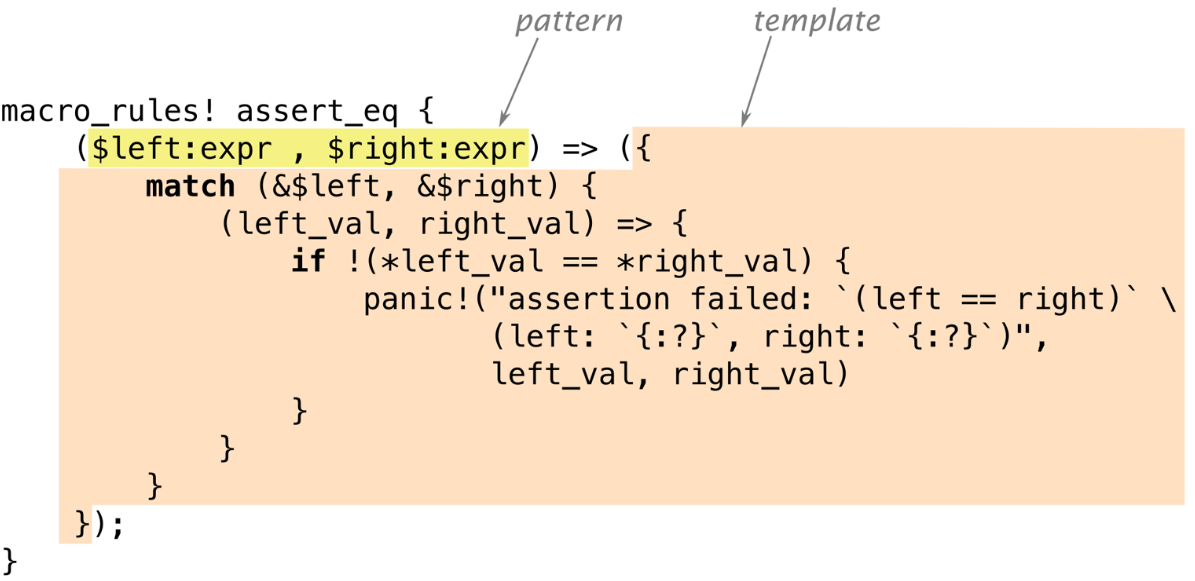
\includegraphics[width=0.9\textwidth]{../img/f21-1.png}
    \caption{\texttt{assert\_eq!}宏}
    \label{f21-1}
\end{figure}

\texttt{macro\_rules!}是Rust中定义宏的主要方法。注意，宏定义里\texttt{assert\_eq}后边没有\texttt{!}：只有在调用宏时才需要\texttt{!}，定义时不需要。

并不是所有的宏都是以这种方式定义的：少数的宏，例如\texttt{file!}、\texttt{line!}和\texttt{macro\_rules!}自身，是编译器内建的。我们将在本章的末尾讨论另一种方法，称为过程宏。但我们的主要精力还是集中在\texttt{macro\_rules!}，这是（目前为止）最容易的编写自己的宏的方法。

一个用\texttt{macro\_rules!}定义的宏完全靠模式匹配工作。宏的主体只是一系列规则：
\begin{minted}{text}
    ( pattern1 ) => ( template1 );
    ( pattern2 ) => ( template2 );
    ...
\end{minted}

\autoref{f21-1}中的\texttt{assert\_eq!}版本只有一个模式和一个模板。

顺便，你可以使用方括号或者花括号来代替模式或模板两侧的圆括号，对Rust来说它们并没有任何区别。另外，当你调用一个宏时，这些都是等价的：
\begin{minted}{Rust}
    assert_eq!(gcd(6, 10), 2);
    assert_eq![gcd(6, 10), 2];
    assert_eq!{gcd(6, 10), 2}
\end{minted}

唯一的不同是花括号后边的分号是可选的。为了方便，我们在调用\texttt{assert\_eq!}时使用圆括号，调用\texttt{vec!}时使用方括号，\texttt{macro\_rules!}时使用花括号。

现在我们展示了一个宏展开的简单示例和生成这个宏的定义，我们可以深入了解它工作的细节：
\begin{itemize}
    \item 我们将详细地解释Rust是怎么发现和展开你的程序中的宏定义的。
    \item 我们将指出在根据宏模板生成代码时的一些细节之处。
    \item 最后，我们将展示模式如何处理重复的结构。
\end{itemize}

\subsection{宏展开基础}
Rust会在编译的前期展开宏。编译器会从头到尾读取源码，在这个过程中定义和展开宏。宏只有在定义之后才能被调用，因为Rust会立刻展开每一个宏调用，而不会去看程序的剩余部分。（相反，函数和其他的\hyperref[static]{item}的定义不需要按照任何顺序。调用一个后面才定义的函数也是OK的。

当Rust展开一个\texttt{assert\_eq!}宏调用时，行为和执行一个\texttt{match}表达式非常像。Rust首先根据模式匹配参数，如\autoref{f21-2}所示：
\begin{figure}[htbp]
    \centering
    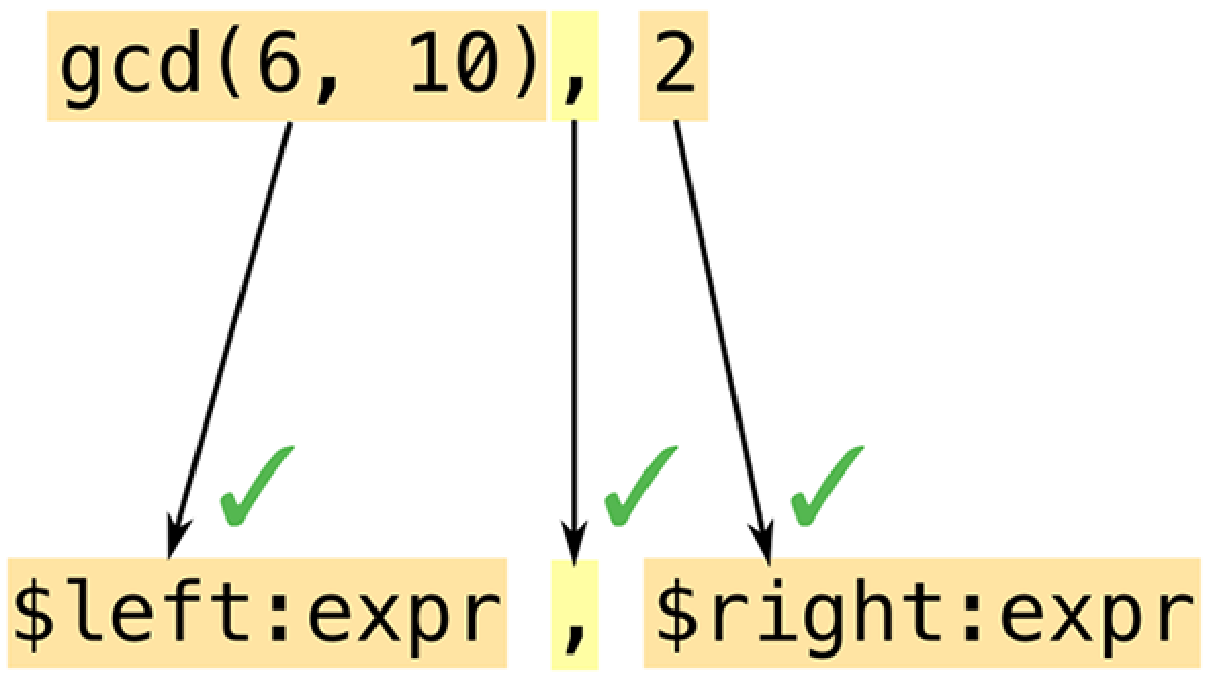
\includegraphics[width=0.8\textwidth]{../img/f21-2.png}
    \caption{展开一个宏，第1部分：用模式匹配参数}
    \label{f21-2}
\end{figure}

宏的模式是Rust的mini语言。它们本质上是匹配代码的正则表达式。但普通的正则表达式是操作字符，而模式操作\emph{token(词元)}——数字、变量名、标点符号等Rust中的构建块。这意味着你可以在宏模式中自由地使用注释和空格来提升它们的可读性。注释和空格不是token，因此它们不会影响到匹配。

正则表达式和宏模式的另一个重要不同之处是圆括号、方括号、花括号在Rust中总是成对出现。这一点会在宏展开之前就检查，不仅仅是在宏模式中，而且是在整个语言中。

在这个例子中，我们的模式包含了\emph{fragment(片段)} \texttt{\$left:expr}，这告诉Rust去匹配一个表达式（在这个例子中，就是\texttt{gcd(6, 10)}并把它复制到名称\texttt{\$left}。然后Rust用\texttt{gcd}调用后边的逗号匹配模式中的逗号。类似于正则表达式，模式只有少数特殊字符会触发有趣的匹配行为；其它的所有字符，例如逗号，都必须逐字匹配相同的字符，否则就会匹配失败。

这个模式中的两个代码片段都是\texttt{expr}类型：它们代表表达式。我们将在“\nameref{FragType}”中看到其他类型的代码片段。

因为这个模式匹配到了所有的参数，Rust会展开相应的\emph{template(模板)}(\autoref{f21-3})：
\begin{figure}[htbp]
    \centering
    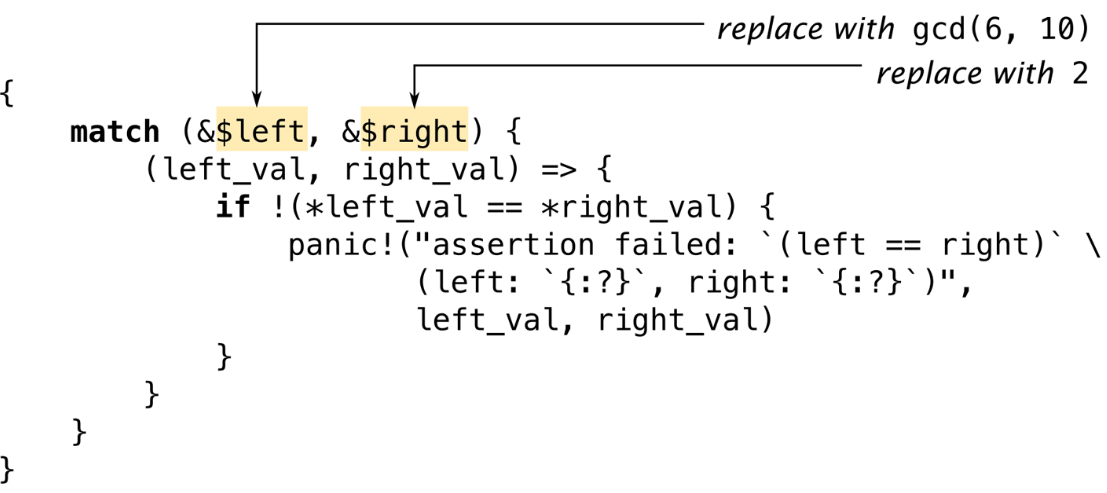
\includegraphics[width=0.9\textwidth]{../img/f21-3.png}
    \caption{展开一个宏，第2部分：填充模板}
    \label{f21-3}
\end{figure}

Rust会用匹配阶段发现的代码片段来替换\texttt{\$left}和\texttt{\$right}。

一个常见的错误是在输出模板中包含片段的类型：写\texttt{\$left:expr}而不是\texttt{\$left}。Rust不会立刻检测出这种错误。它会把\texttt{\$left}看错一个整体，然后把\texttt{:expr}看作和模板中其他部分一样的东西：要包含在宏的输出中的词元。因此只有当你\emph{调用}这个宏时这个错误才会出现；然后它会生成错误的不能编译的输出。如果你在使用一个新的宏时得到了类似\texttt{cannot find type `expr` in this scope}和\texttt{help: maybe you meant to use a path separator here}这样的错误消息，可以检查下它是不是有这个错误。（“\nameref{DebugMacro}”提供了更多类似这种情况的建议。）

宏模板和web编程中常用的很多种模板语言中的任意一种都没有太大的区别。唯一的不同——也是很重要的一点——就是它的输出是Rust代码。

\subsection{意外的结果}
把代码片段插入模板和普通的处理值的代码有一些区别。这些区别一开始可能并不明显。我们之前看到的\texttt{assert\_eq!}宏包含了一些有些奇怪的代码，这是宏编程特有的。让我们重点看看其中两个有趣的部分。

首先，为什么这个宏创建了两个变量\texttt{left\_val}和\texttt{right\_val}？为什么我们不能把模板简化成这样？
\begin{minted}{Rust}
    if !($left == $right) {
        panic!("assertion failed: `(left == right)` \
                (left: `{:?}`, right: `{:?}`)", $left, $right)
    }
\end{minted}
为了回答这个问题，尝试手动展开宏调用\texttt{assert\_eq!(letters.pop(), Some('z'))}。输出将会是什么？Rust会把匹配到的表达式插入模板中的多个位置。看起来在构建错误消息时重新求值表达式是一个坏主意，原因不仅仅是因为它需要消耗两倍的时间：因为\texttt{letters.pop()}从vector中移除一个值，所以在我们第二次调用它时会产生一个和第一次不同的值！这就是为什么真正的宏只计算一次\texttt{\$left}和\texttt{\$right}，然后存储它们的值。

来到第二个问题：为什么这个宏借用了\texttt{\$left}和\texttt{\$right}的值的引用？为什么不直接把它们的\emph{值}存进变量中，像这样？
\begin{minted}{Rust}
    macro_rules! bad_assert_eq {
        ($left:expr, $right:expr) => ({
            match ($left, $right) {
                (left_val, right_val) => {
                    if !(left_val == right_val) {
                        panic!("assertion failed" /* ... */);
                    }
                }
            }
        });
    }
\end{minted}

对于我们展示过的特殊情况，即宏的参数是整数的情况下，这可以正常工作。但如果调用者传递了一个\texttt{String}变量作为\texttt{\$left}或\texttt{\$right}，这段代码将会移动变量的值！
\begin{minted}{Rust}
    fn main() {
        let s = "a rose".to_string();
        bad_assert_eq!(s, "a rose");
        println!("confirmed: {} is a rose", s);    // error: use of moved value "s"
    }
\end{minted}

因为我们不想让断言移动值，所以宏里使用了引用。

（你可能想知道为什么这个宏使用了\texttt{match}而不是\texttt{let}来定义变量。我们也想知道。事实证明并没有特殊的原因这么做。\texttt{let}是等价的。）

简而言之，宏可能做出令人惊讶的行为。如果一个你写的宏附近发生了奇怪的事，那很可能是这个宏有问题。

C++里的这个经典bug你\emph{将不会}看到：
\begin{minted}{Rust}
    // buggy C++ macro to add 1 to a number
    #define ADD_ONE(n) n + 1
\end{minted}

原因大部分的C++程序员应该很熟悉了，并且不值得详细解释，类似\texttt{ADD\_ONE(1) * 10}或者\texttt{ADD\_ONE(1 << 4)}这样的代码可能会产生令人惊讶的行为。为了修复它，你需要在宏定义中加上更多括号。这在Rust中是不必要的，因为Rust宏和语言集成的更好。Rust知道它什么时候是在处理表达式，因此在把一个表达式粘贴到另一个地方时它会自动添加括号。

\subsection{重复}
标准的

\section{内建的宏}


\section{调试宏}\label{DebugMacro}


\section{构建\texttt{json!}宏}


\subsection{片段类型}\label{FragType}

\chapter{unsafe代码}\label{ch22}

\emph{Let no one think of me that I am humble or weak or passive; \\
Let them understand I am of a different kind: dangerous to my enemies, loyal to my friends. \\
To such a life glory belongs.}

系统级编程的乐趣在于，在每一个安全的语言和精心设计的抽象之下，都是不安全的机器语言和比特位。你也可以在Rust中写出这样的代码。

到目前为止本书中介绍的语言部分，例如类型、生命周期、约束检查等都可以自动保证你的程序完全没有内存错误和数据竞争。但这种自动的技术有它的局限性；Rust并不能识别出来很多有价值的技术是安全的。

\emph{unsafe代码}让你可以告诉Rust，“我要使用一些你不能保证安全的特性”。把一个块或者函数标记为unsafe之后，你就可以调用标准库中的\texttt{unsafe}函数、解引用unsafe指针、调用其他语言例如C和C++编写的函数等。Rust的其他安全性检查依然生效：类型检查、生命周期检查、约束检查等仍然和之前一样。unsafe代码只是允许了一小部分额外的特性。

正是因为有了允许超出safe Rust界限的能力，Rust才能实现它自身的大部分基础特性，和C/C++一样，Rust也被用来实现它自己的标准库。unsafe代码可以让\texttt{Vec}类型更高效地管理它的缓冲区；让\texttt{std::io}模块和操作系统交互；让\texttt{std::thread}和\texttt{std::sync}模块提供并发原语。

本章介绍了unsafe特性的一些基础：

\begin{enumerate}
    \item Rust的\texttt{unsafe}块区分开了普通的safe Rust代码和使用unsafe特性的代码。
    \item 你可以把函数标记为\texttt{unsafe}，提醒调用者他们必须遵守的一些额外约束来避免未定义行为。
    \item 原始指针和它们的方法运行对内存进行不受限的访问，并允许你构建Rust的类型系统可能禁止的数据结构。Rust的引用虽然安全，但却是受限制的，原始指针正如每个C或C++程序员所知，是一个强大而锋利的工具。
    \item 理解未定义行为的定义将会帮助你理解为什么它们比得到错误结果还要糟糕的多。
    \item unsafe trait，类似于\texttt{unsafe}函数，隐含了每个实现（而不是每个调用者）都要遵守的规则。
\end{enumerate}

\section{unsafe从何而来？}
在本书的开头处，我们曾经展示过一个C程序，它以一种非常令人惊讶的方式崩溃。这是因为它违背了C标准的一个规则。你可以在Rust中实现相同的效果：

\begin{minted}{bash}
    $cat crash.rs
    fn main() {
        let mut a: usize = 0;
        let ptr = &mut a as *mut usize;
        unsafe {
            *ptr.offset(3) = 0x7ffff72f484c;
        }
    }
    $ cargo build
       Compiling unsafe-samples v0.1.0
        Finished debug [unoptimized + debuginfo] target(s) in 0.44s
    $ ../../target/debug/crash
    crash: Error: .netrc file is readable by others.
    crash: Remove password or make file unreadable by others.
    Segmentation fault (core dumped)
    $
\end{minted}

这个程序借用了局部变量\texttt{a}的一个可变引用，然后把它转换成了\texttt{*mut usize}类型的原始指针，然后使用了它的\texttt{offset}方法来产生一个指向三个字之后的位置的指针。这里恰巧存储了\texttt{main}的返回地址。这个程序用一个常量覆盖了返回地址，因此从\texttt{main}返回之后程序的行为就很奇怪。这个崩溃之所以可行，是因为程序错误使用了unsafe的特性——在这个例子中，就是解引用原始指针的能力。

一个unsafe特性通常隐含了一份\emph{合约（contract）}：即一组Rust不能自动强制，但你必须遵守才能避免\emph{未定义行为}的规则。

一份合约超出了普通的类型检查和生命周期检查，它们隐含着一些unsafe特性特定的规则。通常来说，Rust本身完全不知道这些合约，它们只在unsafe特性的文档里得到解释。例如，原始指针类型的合约是禁止解引用一个指向的位置超出原来指向物的末尾的原始指针。这个例子中的表达式\texttt{*ptr.offset(3) = ...}打破了这个合约。但是，正如上面所示，Rust没有任何警告，成功编译了这个程序：它的安全检查并没有检测出来这个违规行为。当你使用unsafe特性时，你作为程序员，需要负责检查你的代码遵守了它们的合约。

很多特性如果想正确使用，都要遵守一定的规则。但这些规则并不是我们这里说的合约，除非它们可能会导致未定义行为。未定义行为是一种Rust假设你的代码中绝对不会出现的行为。例如，Rust假设你不会用别的值覆盖函数的返回地址。通过了Rust通常的安全检查并且遵守了使用到的unsafe特性的合约的代码不可能会出现这样的行为。因为这个程序违反了原始指针的合约，因此它的行为变得未定义，并最终崩溃。

如果你的代码出现了未定义行为，说明你打破了你负责的一部分，Rust拒绝预测结果。从系统库的深处抛出来一个错误并崩溃是一种可能的结果；把你的计算机的控制权交给攻击者是另一种可能的结果。不同的Rust版本可能也会有不同的行为。然而，有时未定义行为不一定会产生可见的结果。例如，如果这里的\texttt{main}函数永远不会返回（可能调用了\texttt{std::process::exit}）来提前终止程序），那么错误的返回地址也无关紧要。

你只能在\texttt{unsafe}块或者\texttt{unsafe}函数里使用unsafe特性；我们将在接下来的小节介绍它们。它们让unsafe特性不容易被忽略：通过强迫你写一个\texttt{unsafe}块或者函数，Rust能确保你知道你的代码可能要遵守一些额外的规则。

\section{unsafe块}
\texttt{unsafe}块看起来就像一个以\texttt{unsafe}关键字开头的普通块，区别在于你可以在unsafe块里使用unsafe特性：
\begin{minted}{Rust}
    unsafe {
        String::from_utf8_unchecked(ascii)
    }
\end{minted}

如果没有块前面的\texttt{unsafe}关键字，Rust将会禁止使用\texttt{from\_utf8\_unchecked}，因为它是一个\texttt{unsafe}的函数。在\texttt{unsafe}块中，你可以随意使用它。

和普通的Rust块一样，\texttt{unsafe}块的值也是最后一条表达式的值，或者是\texttt{()}。这个例子中\texttt{String::from\_utf8\_unchecked}的调用提供了块的值。

一个\texttt{unsafe}块为你解锁了5个额外的功能：
\begin{enumerate}
    \item 你可以调用\texttt{unsafe}函数。每一个\texttt{unsafe}函数都有它自己的合约，这取决于它的功能。
    \item 你可以解引用原始指针。safe代码可以传递、比较、通过引用转换创建原始指针，但只有unsafe代码才可以使用它们来访问内存。我们将在\nameref{rawp}中详细介绍原始指针并解释如何安全地使用它们。
    \item 你可以访问\texttt{union}的字段，尽管编译器不能确定它们含有相应类型的有效值。
    \item 你可以访问可变的\texttt{static}变量。正如\nameref{globalvar}中解释的一样，Rust不能确保什么时候有线程正在使用可变的\texttt{static}变量，因此它们的合约要求你要确保所有的访问都是正确同步的。
    \item 你可以访问通过Rust的外部函数接口声明的函数和变量。即使它们是不可变的，也会被认为是\texttt{unsafe}的，因为它们是使用其他语言编写的，这些语言可能不遵守Rust的安全规则。
\end{enumerate}

把unsafe特性约束在\texttt{unsafe}块里并不会真的阻止你做任何想做的事。你完全只需要在你的代码里加上一个\texttt{unsafe}块，然后就可以继续了。这个规则的作用主要是为了把人类的注意力吸引到那些Rust不能保证安全性的代码上：
\begin{enumerate}
    \item 你不会意外地使用到unsafe特性，然后发现你要为甚至不知道它的存在的合约负责。
    \item 一个\texttt{unsafe}块可以吸引reviewer更多的注意力。一些项目甚至有一些自动化流程来确保这一点，例如标记出会影响\texttt{unsafe}块的代码来吸引更多注意力。
    \item 当你正在考虑编写一个\texttt{unsafe}块时，你可以花费一点时间来问问自己你的任务是否真的需要这些特性。如果是为了性能，你是否有测量数据表明这真的是一个性能瓶颈？可能有一种在safe Rust中也可以实现相同效果的方法。
\end{enumerate}

\section{示例：一个高效的ASCII字符类型}
这里有一个示例，\texttt{Ascii}是一个字符串类型，它确保它的内容总是有效的ASCII字符。这个类型使用一个unsafe特性来提供到\texttt{String}的0开销转换：
\begin{minted}{Rust}
    mod my_ascii {
        /// 一个ASCII编码的字符串
        #[derive(Debug, Eq, PartialEq)]
        pub struct Ascii(
            // 它必须只存有有效的ASCII文本：从`0`到`0x7f`的字节序列
            Vec<u8>
        );

        impl Ascii {
            /// 从`bytes`中的Ascii文本创建一个`Ascii`。
            /// 如果`bytes`中含有任何非ASCII字符就返回一个`NotAsciiError`错误。
            pub fn from_bytes(bytes: Vec<u8>) -> Result<Ascii, NotAsciiError> {
                if bytes.iter().any(|&byte| !byte.is_ascii()) {
                    return Err(NotAsciiError(bytes));
                }
                Ok(Ascii(bytes))
            }
        }

        // 当转换失败时，我们会给出不能转换的vector。
        // 它应该实现`std::error::Error`，这里为了简洁就省略了。
        #[derive(Debug, Eq, PartialEq)]
        pub struct NotAsciiError(pub Vec<u8>);

        // 安全、高效的转换，使用unsafe代码实现。
        impl From<Ascii> for String {
            fn from(ascii: Ascii) -> String {
                // 如果这个模块没有bug的话，这里就是安全的，
                // 因为有效的ASCII文本也是有效的UTF-8文本。
                unsafe { String::from_utf8_unchecked(ascii.0) }
            }
        }
        ...
    }
\end{minted}

这个模块的关键是\texttt{Ascii}类型的定义。这个类型本身被标记为\texttt{pub}，来让它在\texttt{my\_ascii}模块外可见。但它的\texttt{Vec<u8>}元素\emph{不是}public的，因此只有\texttt{my\_ascii}模块里的方法可以创建一个\texttt{Ascii}值或者访问它的元素。这完全控制了模块里哪些代码是公开的哪些是不公开的。只要public的构造器和方法能确保新创建的\texttt{Ascii}值是有效的，并始终保持有效，那么程序的其他部分就不可能违反规则。并且public的构造器\texttt{Ascii::from\_bytes}确实小心地检查了给定的vector来确保能从它构建出一个有效的\texttt{Ascii}。出于简洁性的考虑，我们并没有展示出每一个方法，但你可以想象还有一些处理文本的方法，这些方法同样确保\texttt{Ascii}的值总是有效的ASCII文本，就像\texttt{String}的方法确保它的内容总是有效的UTF-8.

这样的安排让我们可以非常高效地为\texttt{String}实现\texttt{From<Ascii>}。unsafe函数\texttt{String::from\_utf8\_unchecked}获取一个字节vector并根据它的内容构建一个\texttt{String}，并且不检查它的内容是否是有效的UTF-8文本；这个函数的合约就是调用者要负责这一点。幸运的是，\texttt{Ascii}类型强迫的规则正是满足\texttt{from\_utf8\_unchecked}的合约所需的条件。正如我们在\nameref{utf8}中解释的一样，任何有效的ASCII文本都是有效的UTF-8文本，因此\texttt{Ascii}内部的\texttt{Vec<u8>}可以立刻作为一个\texttt{String}的缓冲区使用。

有了这些定义之后，你可以写这样的代码：
\begin{minted}{Rust}
    use my_ascii::Ascii;

    let bytes: Vec<u8> = b"ASCII and ye shall receive".to_vec();

    // 这里的调用没有任何内存分配或者文本拷贝，只进行一次扫描。
    let ascii: Ascii = Ascii::from_bytes(bytes)
        .unwrap();  // 我们已经知道了bytes是没问题的。

    // 这里的调用是0开销的：没有内存分配、拷贝、扫描。
    let string = String::from(ascii);

    assert_eq!(string, "ASCII and ye shall receive");
\end{minted}

使用\texttt{Ascii}不需要unsafe块。我们已经使用unsafe操作实现了一个safe的接口，并且安排好只依赖模块自己的代码而不是用户的行为来满足它的合约。

\texttt{Ascii}只是一个\texttt{Vec<u8>}的包装，并在模块里隐藏了一些强迫它的内容需要满足的规则。一个这样的类型被称为\emph{newtype}，它是Rust中非常普遍的一种模式。Rust自己的\texttt{String}类型就使用完全相同的方式定义的，区别只有它的内容被限制为UTF-8，而不是ASCII。事实上，这是标准库里\texttt{String}的定义：
\begin{minted}{Rust}
    pub struct String {
        vec: Vec<u8>,
    }
\end{minted}

在机器语言的层面上，是完全没有Rust的类型信息的，一个newtype和它的元素有完全相同的内存表示，因此构建一个newtype完全不需要任何额外的机器指令。在\texttt{Ascii::from\_bytes}中，表达式\texttt{Ascii(bytes)}只是表明\texttt{Vec<u8>}现在的内存表示持有的是一个\texttt{Ascii}值。类似的，\texttt{String::from\_utf8\_unchecked}在内联的情况下可能不包含任何机器指令：它只表明\texttt{Vec<u8>}现在被认为是一个\texttt{String}。

\section{unsafe函数}
\texttt{unsafe}函数的定义就像一个以\texttt{unsafe}开头的普通函数。\texttt{unsafe}函数的函数体自动被认为是一个\texttt{unsafe}块。

你只能在\texttt{unsafe}块里调用\texttt{unsafe}函数。这意味着将一个函数标记为\texttt{unsafe}可以警告调用者这个函数有一个额外的合约，必须满足这个合约才能避免未定义行为。

例如，这里有一个新的\texttt{Ascii}类的构造器，这个构造器从一个字节vector构建一个\texttt{Ascii}，并且不检查内容是否是有效的ASCII：
\begin{minted}{Rust}
    // 这段代码必须放在`my_ascii`模块中。
    impl Ascii {
        /// 从`bytes`构建一个`Ascii`值，不检查`bytes`是否是有效的ASCII文本。
        ///
        /// 这个函数直接返回一个`Ascii`，而不是像`from_bytes`一样返回一个
        /// `Result<Ascii, NotAsciiError>`。
        ///
        /// # 安全性
        ///
        /// 调用者必须确保`bytes`只包含ASCII字符：每个字节都不大于0x7f。
        /// 否则，最后的结果是未定义的。
        pub unsafe fn from_bytes_unchecked(bytes: Vec<u8>) -> Ascii {
            Ascii(bytes)
        }
    }
\end{minted}

如果调用\texttt{Ascii::from\_bytes\_unchecked}的代码总是知道vector中只包含有效的ASCII字符，那么\texttt{Ascii::from\_bytes}里的检查就只是在浪费时间，并且调用者还必须处理永远不会出现的\texttt{Err}结果。\texttt{Ascii::from\_bytes}可以简化这种情况下的调用和错误处理。

但之前我们曾经强调过\texttt{Ascii}的public构造器和方法保证\texttt{Ascii}的值是有效的的重要性。\texttt{from\_bytes\_unchecked}是不是没有遵守这个规则？

不完全是：\texttt{from\_bytes\_unchecked}把它的责任通过它的合约交给了调用者。这个合约的存在正是它应该被标记为\texttt{unsafe}的原因：虽然这个函数本身没有进行unsafe的操作，但它的调用者必须遵守一些Rust不能强制的规则才能避免未定义行为。

你真的能通过打破\texttt{Ascii::from\_bytes\_unchecked}的合约来导致未定义行为吗？是的。你可以像下面这样构造一个无效的\texttt{String}：
\begin{minted}{Rust}
    // 想象这个vector是一些我们认为会产生ASCII文本的操作的结果，
    // 但这个操作出错了。
    let bytes = vec![0xf7, 0xbf, 0xbf, 0xbf];
    let ascii = unsafe {
        // 当`bytes`含有非ASCII值时这个unsafe的合约就被打破了
        Ascii::from_bytes_unchecked(bytes)
    };

    let bogus: String = ascii.into();

    // `bogus` 现在包含无效的UTF-8。
    // 解析它的第一个字符会产生一个无效的Unicode码点的`char`，
    // 这是未定义行为，因此Rust不知道这个断言的行为会是什么样的。
    assert_eq!(bogus.chars().next().unwrap() as u32, 0x1fffff);
\end{minted}

在特定版本的Rust和特定的平台上，这个断言会输出下面的错误信息并失败：
\begin{minted}{text}
    thread 'main' panicked at 'assertion failed: `(left == right)`
      left: `2097151`
     right: `2097151`, src/main.rs:42:5
\end{minted}

这两个数字在我们看来似乎是相等的，但这不是Rust的问题；这是之前的\texttt{unsafe}块的问题。当我们说未定义行为会导致无法预料的结果时，这就是其中一种情况。

这个例子展示了两个有关bug和unsafe代码的关键事实：
\begin{enumerate}
    \item \emph{\texttt{unsafe}块之前发生的bug可能会打破合约}。一个\texttt{unsafe}块是否会导致未定义行为可能不仅仅取决于这个块本身，还取决于提供它要操作的值的代码。你的\texttt{unsafe}代码依赖的任何东西都是和安全相关的。只有当模块的其他部分正确的维护了\texttt{Ascii}相关的内容时，基于\texttt{String::from\_utf\_unchecked}的\texttt{Ascii}到\texttt{String}的转换才是安全的。
    \item \emph{打破合约的结果可能在你离开\texttt{unsafe}块之后才会出现}。不遵守unsafe特性而导致的未定义行为通常不会在\texttt{unsafe}块本身里出现。如上面所示，构造一个bogus \texttt{String}可能不会有问题，直到程序的程序执行中才出现问题。
\end{enumerate}

本质上讲，Rsut的类型检查、借用检查和其他的静态检查都是在分析你的程序并尝试证明它不可能会出现未定义行为。当Rust成功编译你的程序时，这意味着它成功地证明了这一点。一个\texttt{unsafe}块是这个证明中的例外：等于你在告诉Rust“它没有问题，相信我”。你的声明是否正确可能依赖程序的任何会影响到\texttt{unsafe}块的部分，并且出错时产生的结果也可能出现在任何被\texttt{unsafe}块影响的地方。\texttt{unsafe}关键字也是在提醒你，你无法完全享受到它的安全检查的好处。

如果可以选择的话，你应该尽量选择使用安全的没有合约的接口。它们更容易使用，因为用户可以依赖Rust的安全检查来保证他们的代码不可能出现未定义行为。即使你的实现使用了unsafe特性，最好使用Rust的类型、生命周期和模块系统来满足它们的合约，同事只使用你自己就可以保证的，而不是把责任传递给调用者。

不幸的是，在实际编程中遇到懒得解释它们的合约的unsafe函数并不罕见。他们期望你能依靠自己的经验和知识自己推导出这些规则。

\section{unsafe块还是unsafe函数？}
你可能会想知道是使用\texttt{unsafe}块还是直接把整个函数标记为unsafe。我们推荐的方法是首先判断函数：
\begin{enumerate}
    \item 如果这个函数可能被误用，可以成功编译但可能导致未定义行为，那么你应该将它标记为unsafe。正确使用这个函数的规则就是它的合约，也正是合约的存在让它变得unsafe。
    \item 否则，这个函数是safe的：没有调用能让它产生未定义行为。它不应该被标记为\texttt{unsafe}。
\end{enumerate}

这个函数在函数体里是否使用unsafe特性并不这个重要，关键是合约的存在。之前我们展示过一个没有使用unsafe特性的unsafe函数，也展示过一个使用了unsafe特性的safe函数。

不要只因为你在函数体里使用了unsafe特性就把safe的函数标记为\texttt{unsafe}。这只会让函数更难用，并且迷惑调用者，让他以为这里有一个合约。正确的做法是使用一个\texttt{unsafe}块，即使这个块就是整个函数体。

\section{未定义行为}


\section{原始指针}\label{rawp}


\chapter{外部函数}\label{ch23}
\backmatter
\end{document}
